% -*- latex -*-

% Definitions for this chapter.

% -*- latex -*-

% Magic numbers: disk label
\newcommand\DescriptorSize{29}
\newcommand\magicROMBoot{\hex{6400}}
\newcommand\magicCustomBoot{\hex{D010}}
\newcommand\magicDiskLabel{\hex{CF75}}
\newcommand\magicCFTFSType{\hex{F501}}
\newcommand\magicEmptySlice{\hex{FFFF}}

% Magic numbers: filesystem
\newcommand\magicVolume{\hex{CF70}}
\newcommand\magicVolDesc{\hex{CF71}}
\newcommand\magicDirectory{\hex{CF7D}}
\newcommand\magicDirDesc{\hex{CF7E}}
\newcommand\magicFileDesc{\hex{CF7F}}
\newcommand\magicDirectoryCont{\hex{CF7C}}
\newcommand\magicIndexBlock{\hex{CF7B}}

% End of file.


\chapter{Data Storage}
\label{sec:fs}

\begin{figure}
  \centering
  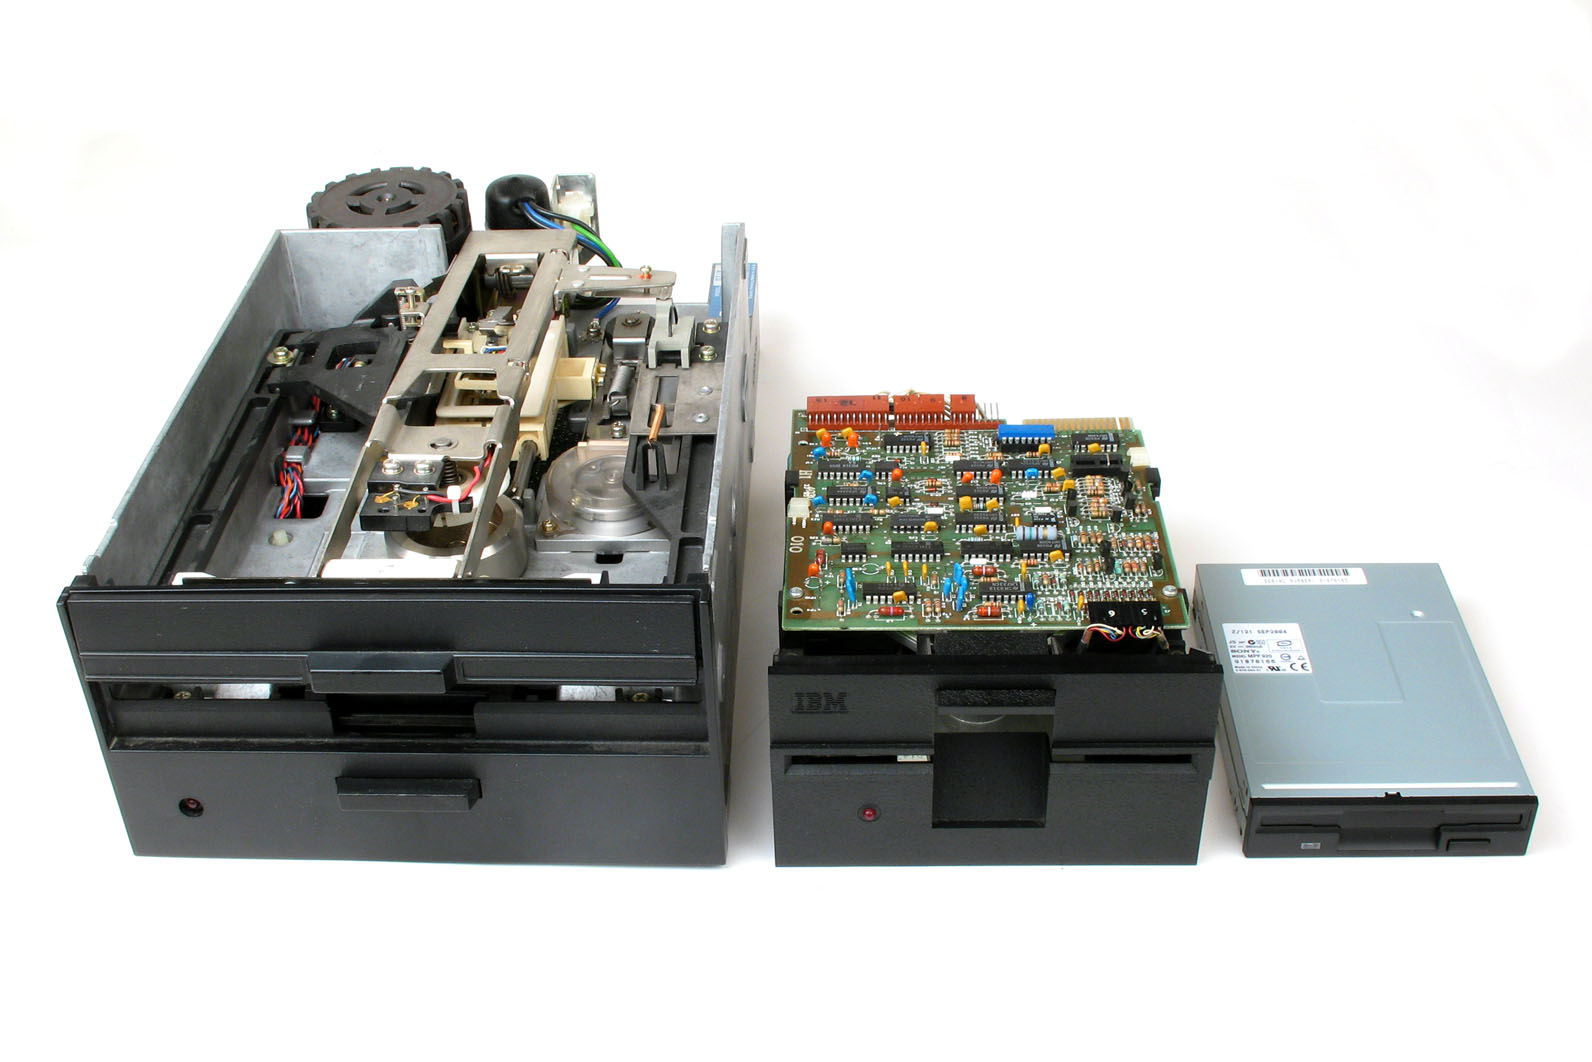
\includegraphics[width=0.75\columnwidth]{figs/Floppy_Disk_Drives_8_5_3.jpg}
  \caption[Floppy drives]{Floppy drives. 8-inch (left), full-height
    5¼-inch (middle), 3½-inch (right). The ‘full-height’ 5¼-inch unit
    is the size of two stacked internal CD/DVD drives (the desktop versions).}
\end{figure}


This chapter describes how CFT storage media are organised. Currently, the only
media in planning are IDE (parallel ATA) disk and disk-like devices such as CF
cards. IDE CD-ROMs may be attached and eventually supported but this is not
planned.

I initially considered supporting floppy drives using one of the older
WD37C65 Floppy Drive Controller chips, which are still relatively easy
to find (used). I have a number of Shugart 8-inch devices and several
of the smaller capacity IBM/Tandon 5¼-inch units, and enough floppy
disks. An immense 8-inch floppy drive controlled by the CFT would be
appropriate and interesting to look at (and provide interesting
mini-computer-like sound effects with its head loading/unloding
sounds), but IDE storage is easier to interface to, more convenient
and devices are simpler to find, attach, and run. The floppy
sub-project is still likely to go ahead, but not as the main means of
storage for the CFT.

A cassette tape interface is much simpler to build than a floppy
controller, and I may attempt this as part of a multi-I/O board for
the novelty factor. Desktop cassette decks of the type used in the
Eighties are not very common and their rubber parts need maintenance
which makes them not age well. Thankfully, analogue audio will always
be with us, and a multitude of devices could be used to store and play
back data streams: from digital voice recorders, to mobile phones and
other computers.

\section{Fundamentals}

Every storage medium is ultimately a memory array. Unlike memory, storage is
addressed in blocks. Standard Forth blocks are always 1,024 bytes (512 words)
in size, but storage blocks are most often 256–4,096 bytes (128–2,048 words) in
size. Storage is accessed in whole blocks, i.e. a block is the quantum of
storage. 

Every medium uses its own way of addressing individual
blocks. Three-dimensional vectors (head, cylinder, sector) are used for
floppies and (at the lowest level) for hard disks. On hard disks, the on-board
controller hides this and presents the disk as a simple array of (almost
always) 256-word blocks.

\section{Units of Measurement}

This discussion (and much of this chapter) often makes reference to
{\em bytes\/} which are defined to be eight-bit quantities. This is
done so that quantities make sense to the average reader, who is used
to multiples of bytes, but not of words. Whenever bytes are
referenced, quantities in Words are also provided. For the purpose of
this chapter, multiples of bytes and words are base two:

\begin{center}
  \zebra
  \begin{tabular}{lll}
    Prefix & Unit    & Description\\\hline
    Kilo-  & kB      & 1 Kilobyte = $2^{10}=1,024$ Bytes (512 Words) \\
    Mega-  & MB      & 1 Megabyte = $2^{20}=1,048,576$ Bytes (512 kWords) \\
    Giga-  & GB      & 1 Megabyte = $2^{30}=1,073,741,824$ Bytes (512 MWords) \\
    Tera-  & TB      & 1 Terabyte = $2^{40}=1,099,511,627,776$ Bytes (512 GWords) \\
    \hline
  \end{tabular}
\end{center}%
%
\noindent This may seem counter to modern practice, but the design of
CFT mirrors the design of similar computers before marketing reasons
made storage device manufacturers decimalise their units. Binary units
make sense for storage devices, since their block sizes are powers of
two, even though the total storage capacity is not. It is, however, a
multiple of a power of two (the block size), and is better expressed
in binary units.

\section{Byte Oriented Storage Media}

Some storage media are byte oriented, others are word oriented. IDE
disk drives use a 16-bit word, which is ideal for use on the CFT
architecture: reading a traditional\footnote{Modern IDE blocks are
  4,096 bytes long.} 512 byte IDE block requires 256 reads from the
drive.

Other devices, like floppy drives, are byte oriented. In this case, for
the typical 512 byte sector, the processor must perform 512 8-bit
transactions using a state machine that shifts the first byte read 8
bits to the right, making it the MSB.

\todo{Check this!}
Byte ordering terms do not apply to a word-oriented machine, but this
makes the CFT a big-endian architecture, at least in the way it reads
from 8-bit devices.

\section{Some Data Structures}

This chapter makes reference to a number of simple (or common) data
structures, which are defined below:

\begin{description}
  \item\simpledatastructure{Word} this is the familiar 16-bit quantity, the
    smallest amount of data the CFT can access from memory. Words represent
    values in the range 0–65,535.
  \item\simpledatastructure{Cell} same as \ds{Word}. Used when discussing
    Forth.
  \item\simpledatastructure{Code} one or more 16-bit words representing CFT
    instructions.
  \item\simpledatastructure{DWord} short for ‘double word’. This is a sequence
    of two words representing an unsigned, 32-bit integer. The \gls{MSB} is the
    first word (lowest offset or address). A \ds{DWord} can represent values in
    the range 0–4,294,967,295.
  \item\simpledatastructure{Reserved} not a true data structure. This is used
    to mark one or more words that are reserved for future expansion.
  \item\simpledatastructure{Date} A 16-bit value representing a date. This is a
    bitfield with the following structure\footnote{Readers with a good memory
      or traumatic experiences will identify this as the same data structure
      used by MS-DOS. This is pure co-incidence, guided by the fact that MS-DOS
      was 16-bit, and the Gregorian calendar hasn't changed much since the late
      1970s.}:

    \begin{cbitfield}
      \bitfieldItem{5}{cfthl!50}{Day}
      \bitfieldItem{4}{cfthl!25}{Month}
      \bitfieldItem{7}{cfthl!50}{Year}
    \end{cbitfield}

    \begin{description}
      \item {\bfseries Day:} the day of the month as an unsigned integer in the range 1–31.
      \item {\bfseries Month:} the month as an unsigned integer in the range 1–12.
      \item {\bfseries Year:} the year as an unsigned integer in the range
        0–127. The CFT Epoch Year, 1960, is added to this, to allow years in
        the range 1960–2087.
    \end{description}

  \item\simpledatastructure{Time} A 16-bit value representing a timestamp. This
    is a bitfield with the following structure\footnote{Again, this is
      identical to the MS-DOS timestamp due to the similarity in limits and
      requirements.}:

    \begin{cbitfield}
      \bitfieldItem{5}{cfthl!50}{Seconds}
      \bitfieldItem{6}{cfthl!25}{Minutes}
      \bitfieldItem{5}{cfthl!50}{Hours}
    \end{cbitfield}

    \begin{description}
      \item {\bfseries Seconds:} the seconds of the timestamp in the range
        0–31. Note that this range is unable to represent the required 0–59
        range. Seconds are shifted one bit to the right, effectively multiplied
        by two. This gives a range of 0–58 in increments of two. The CFT can
        thus record timestamps with a precision of 2 seconds. This is
        sufficient for many needs. MS-DOS did the same and few users noticed
        the low accuracy.
      \item {\bfseries Minutes:} the minutes of the timestsamp in the range
        0–59.
      \item {\bfseries Hours:} the hours of the timestamp, in the range 0–23
        (24-hour format).
    \end{description}

  \item\simpledatastructure{PString} this data structure occupies one or more
    words, depending on its use. It is used to hold a CFT packed string, a
    compact method of recording strings of identifier characters. Packed
    strings contain 127-bit US ASCII values. Every word contains two such
    characters. Odd-numbered characters take up the lower 8 bits, even-numbered
    characters take up the upper 8 bits. The last character in the string is
    denoted by setting the eighth bit (\cftcode{END}) for any character:

    \begin{cbitfield}
      \bitfieldGroup{7}{cfthl!50}{Character index 0}
      \bitfieldItem{1}{cfthl!25}{END}
      \bitfieldGroup{7}{cfthl!50}{Character index 1}
      \bitfieldItem{1}{cfthl!25}{END}
    \end{cbitfield}

    Packed strings are also discussed in~\cf{sec:asm-pstring}.

  \item\simpledatastructure{BlockPtr} this is a \ds{DWord} value: a 32-bit
    unsigned integer, MSB first. It is interpreted as a pointer to a block
    within a volume. Non-zero values refer to a block by its number. A zero
    (\hex{00000000}) denotes the pointer \cftcode{NULL} value, usually
    interpreted as ‘no block’ in this context.
\end{description}

In addition, a complex data structure, \ds{DateTime} is defined to record the
date and time of a timestamp:

\begin{datastructure}[Offset]{DateTime}
    \dsdesc{\hex{00}}{Date}{%
      The \ds{Date} part of the timestamp.
      }
    %
    \dsdesc{\hex{01}}{Time}{%
      The \ds{Time} part of the timestamp.
    }
    %
\end{datastructure}


\section{Translating Native Geometry to Block Addresses}

Most physical storage devices are block-oriented, but their blocks are
addressed in native schemes. Functions are provided to map from these
native schemes to block counts (and the reverse).

\subsection{IDE Hard Drives}

IDE hard drives traditionally used a three-dimensional cylinder-head-sector
addressing scheme. All but the oldest IDE-compatible drives also provide a
block-level view of the disk. The disk's embedded controller is responsible for
the mapping from one scheme to the other, so the CFT operating system does not
need to.

\subsection{Floppy Disks}

Floppy disks always use cylinder-head-sector addressing, but floppy disk
controllers do not provide a logical block mapping in hardware. The operating
system must provide a mapping function in software. One complication here is
that the number of cylinders and sectors are not necessarily powers of two, so
software multiplications or an in-memory offset table would be needed.

%% This can be avoided by padding cylinders and sectors to a power of two, and
%% using the entire vector as a block number. Floppy cylinders are commonly in the
%% range 0–40 to 0–80. 7 bits can be used for this. Sector numbers start at 1. The
%% number of sectors per track differs between floppy drive technology, but 5 bits
%% would be more than enough. The head ordinate is either 0 or 1. One mapping
%% function could thus be $64c + 32h + s - 1$. This allows a sparse, 13-bit block
%% map. To avoid allocating 

\subsection{Tapes}

Tapes are sequential access devives and are operated at the pulse level. There
are blocks, and tapes cannot hold a CFT filesystem, so no block translation is
needed.

\section{Disk Label}
\label{sec:disk-label}
\label{sec:disklabel}
\label{sec:disk-slices}

All disks, including floppy disks, have a \gls{disk label}. The disk
label is at block 0 of the device. It identifies the device as
properly prepared for use. It contains the magic number
\magicDiskLabel (used to detect the presence of the disk label), space
for 126 words of optional boot code, and defines between one and
sixteen \glspl{disk slice}.

\begin{figure}
 \centering
 % -*- latex -*-
\documentclass[class=memoir,border=200pt]{standalone}
% -*- latex -*-

%%%%%%%%%%%%%%%%%%%%%%%%%%%%%%%%%%%%%%%%%%%%%%%%%%%%%%%%%%%%%%%%%%%%%%%%%%%%%%%
%%
%% PACKAGES
%%
%%%%%%%%%%%%%%%%%%%%%%%%%%%%%%%%%%%%%%%%%%%%%%%%%%%%%%%%%%%%%%%%%%%%%%%%%%%%%%%

\usepackage{ifxetex}
\usepackage{graphicx}

\usepackage{verbatim}
\usepackage{ifthen}
\usepackage{float}
\usepackage{floatflt}
\usepackage{lipsum}
\usepackage{layout}
\usepackage{calc}
\usepackage{rotating}
\usepackage{array}
\usepackage{color}
\usepackage[table]{xcolor}
\usepackage[includefoot]{geometry}

% Conditional packages
\ifxetex
  % Load fontspec and set fonts
  \usepackage{fontspec}
  \setmainfont{Minion Pro}
  \setsansfont{Myriad Pro}
  \setmonofont[]{Inconsolata}

  \usepackage{pdftricks}
  \usepackage{pdfpages}

  \def\HCode#1{}

\else
  \newcounter{Hfootnote}
  \newcommand\fontspec[1]{}
  %\usepackage[main=english,greek]{babel}
  \usepackage[utf8]{inputenc}
  \usepackage{newunicodechar}
  \newunicodechar{®}{\HCode{&reg;}}
  \newunicodechar{µ}{\HCode{&mu;}} % ‘micro’ (from latin-1 plane)
  \newunicodechar{μ}{\HCode{&mu;}} % mu (from Greek plane)
  \newunicodechar{–}{--}
  \newunicodechar{—}{---}
  \newunicodechar{×}{\ensuremath{\times}}
  \newunicodechar{°}{\HCode{&deg;}}
  \newunicodechar{±}{\HCode{&plusm;}}
  \newunicodechar{Ω}{\ensuremath{\Omega}}
  \newunicodechar{÷}{\ensuremath{\div}}
  %\newunicodechar{²}{\HCode{&sup2;}}
  \newunicodechar{²}{*2*}
  \newunicodechar{¼}{\HCode{&\#188;}}
  \newunicodechar{½}{\HCode{&\#189;}}
  \newunicodechar{≤}{\HCode{ &le; }}
  \newunicodechar{≥}{\HCode{ &ge; }}
  \newunicodechar{≠}{\HCode{ &ne; }}
\fi

%%%%%%%%%%%%%%%%%%%%%%%%%%%%%%%%%%%%%%%%%%%%%%%%%%%%%%%%%%%%%%%%%%%%%%%%%%%%%%%
%%
%% TABLES
%%
%%%%%%%%%%%%%%%%%%%%%%%%%%%%%%%%%%%%%%%%%%%%%%%%%%%%%%%%%%%%%%%%%%%%%%%%%%%%%%%

\renewcommand*\arraystretch{1.25}
\newcolumntype{P}[1]{>{\raggedright\arraybackslash}p{#1}}


%%%%%%%%%%%%%%%%%%%%%%%%%%%%%%%%%%%%%%%%%%%%%%%%%%%%%%%%%%%%%%%%%%%%%%%%%%%%%%%
%%
%% FIGURE DRAWING WITH PGF/TIKZ
%%
%%%%%%%%%%%%%%%%%%%%%%%%%%%%%%%%%%%%%%%%%%%%%%%%%%%%%%%%%%%%%%%%%%%%%%%%%%%%%%%

\ifxetex
  \usepackage{pgf}
  \usepackage{tikz}
  \usepackage{rotating}
  \usepackage[absolute]{textpos}

  %\usetikzlibrary{arrows,positioning,automata,shadows,fit,shapes,counters}
  \usetikzlibrary{arrows,positioning,automata,shadows,fit,shapes,patterns}
  \usetikzlibrary{shadows.blur}
  %\usetikzlibrary{external}
  %\tikzexternalize[prefix=tikz/]
  %\tikzset{external/system call={xelatex \tikzexternalcheckshellescape -halt-on-error -interaction=batchmode -jobname "\image" "\texsource"}}
  \usepackage{standalone}

  \usepackage{tikz-timing}[2009/07/28]
  \usetikztiminglibrary{either}[2009/07/28]
  \tikzset{>=latex}
  \tikzset{timing/z/.append style={black},}
  \tikzset{timing/.append style={x=1ex, y=2ex, line cap=round, line join=round, line width=1.3pt}}
  \tikzset{timing/slope=0.33}
  \tikzstyle{semithick}=[line width=1pt]
  \tikzstyle{heavy}=[line width=2pt]
  \tikzstyle{heavy outline}=[line width=3.5pt]
  \tikzstyle{plot line}=[line width=4pt]
  \tikzstyle{arrow}=[semithick]
  \tikzstyle{thick arrow}=[heavy]
  \tikzstyle{thick outline arrow}=[thick arrow, heavy outline, color=white, draw opacity=0.8]
  \tikzstyle{help lines}=[dotted, line width=0.5pt]
  \tikzstyle{col1}=[draw=p1,fill=p1!60]
  \tikzstyle{col2}=[draw=p2,fill=p2!60]
  \tikzstyle{col3}=[draw=p3,fill=p3!60]
  \tikzstyle{col4}=[draw=p4,fill=p4!60]
  \tikzstyle{col5}=[draw=p5,fill=p5!60]
  \tikzstyle{col6}=[draw=p6,fill=p6!60]
  \tikzstyle{dropshadow}=[] % shade,blur shadow={shadow blur steps=5, shadow blur extra rounding=1.3pt}]
  \tikzset{fsmstate/.style={state,rectangle,rounded corners,dropshadow,minimum width=10em,line width=1pt}}
  % Create a hatch pattern
  \newlength{\hatchspread}
  \newlength{\hatchthickness}
  % declaring the keys in tikz
  \tikzset{hatchspread/.code={\setlength{\hatchspread}{#1}},
           hatchthickness/.code={\setlength{\hatchthickness}{#1}}}
  \tikzset{hatchspread=3pt,
           hatchthickness=0.4pt}
  \pgfdeclarepatternformonly[\hatchspread,\hatchthickness]% variables
     {hatch}% name
     {\pgfqpoint{-2\hatchthickness}{-2\hatchthickness}}% lower left corner
     {\pgfqpoint{\dimexpr\hatchspread+2\hatchthickness}{\dimexpr\hatchspread+2\hatchthickness}}% upper right corner
     {\pgfqpoint{\hatchspread}{\hatchspread}}% tile size
     {% shape description
      \pgfsetlinewidth{\hatchthickness}
      \pgfpathmoveto{\pgfqpoint{0pt}{\hatchspread}}
      \pgfpathlineto{\pgfqpoint{\dimexpr\hatchspread+0.15pt}{-0.15pt}}
      \pgfusepath{stroke}
     }
\fi


%%%%%%%%%%%%%%%%%%%%%%%%%%%%%%%%%%%%%%%%%%%%%%%%%%%%%%%%%%%%%%%%%%%%%%%%%%%%%%%
%%
%% HYPERREF
%%
%%%%%%%%%%%%%%%%%%%%%%%%%%%%%%%%%%%%%%%%%%%%%%%%%%%%%%%%%%%%%%%%%%%%%%%%%%%%%%%

\makeatletter
\@ifpackageloaded{standalone}{}{
  \ifxetex
    \usepackage[CJKbookmarks,bookmarks=true,bookmarksopen=true,pdfpagelabels,pdfstartpage=1]{hyperref}
  \else
    \usepackage[tex4ht]{hyperref}
  \fi
}

\let\old@part\part
\renewcommand\part[1]{%
  \setcounter{chapter}{0}%
  \old@part{#1}%
}
%\renewcommand*{\theHchapter}{\thepart.\thechapter}
\makeatother


%%%%%%%%%%%%%%%%%%%%%%%%%%%%%%%%%%%%%%%%%%%%%%%%%%%%%%%%%%%%%%%%%%%%%%%%%%%%%%%
%%
%% INDEX AND GLOSSARY
%%
%%%%%%%%%%%%%%%%%%%%%%%%%%%%%%%%%%%%%%%%%%%%%%%%%%%%%%%%%%%%%%%%%%%%%%%%%%%%%%%

\usepackage{makeidx}
% Glossaries
\usepackage[acronym]{glossaries}
%\makeindex
%\makeglossaries
% -*- latex -*-

\renewcommand\glspostdescription{}

\newcommand\newglossaryabbr[3]{%
  \newglossaryentry{abbr#1}{name=\glslink{#1}{#2}, text={#2}, description={#3}}
  \newacronym[description={\glslink{abbr#1}{#2}}]{#1}{#1}{#2}
}

\newglossaryentry{IBUS}{name=IBUS,
  description={
  Internal Bus: the single, internal 16-bit bus of the CFT processor.
  }}
  
\newglossaryentry{Data Bus}{name=Data Bus, description={ A
    16-bit bus used to move data between the processor and
    peripherals.  }}
  
\newglossaryentry{Address Bus}{name=Address Bus, description={A
    16-bit bus used to select a peripheral nor memory location to
    access.}}
  
\newglossaryentry{Video Display Unit}{name=Video Display Unit,
  description={ Video Display Unit (VDU): a device that drives a
    display monitor to show character or graphics data on a
    screen. Often also contains one or more input devices (keyboard,
    mouse).}}
  
\newglossaryentry{von Neumann architecture}{name=Von Neumann architecture,
  description={ Named after the work of
    John von Neumann, the von Neumann architecture is a ‘modern’
    computer architecture that includes a register file, arithmetic
    and logic units, memory and input/output, and uses the same
    storage for programs and data.}}

\newglossaryentry{stored program computer}{name=Stored program computer,
  description={ A type of computer that
    uses the same storage for programs and data. All modern computers
    are stored program computers, allowing self-modification of their
    programs. Early designs and many modern microcontrollers stored
    programs and data in separate media, and did not or could not
    treat programs as data.}}

\newglossaryabbr{ALU}{Arithmetic/Logic Unit}{Describe this!}
\newglossaryabbr{ISR}{Interrupt Service Routine}{Describe this!}
\newglossaryentry{UART}{name=UART, description={
    Short for Universal Asynchronous Receiver/Transmitter. UARTs are
    devices that handle asynchronous serial communications such as RS-232, RS-485 or USB.
    }
}
%% \newglossaryentry{alu}{name=\glslink{ALU}{Arithmetic/Logic Unit}, text=Arithmetic/Logic Unit,
%%   description={TODO}}
%% \newacronym[description={\glslink{alu}{Arithmetic/Logic Unit}}]{ALU}{ALU}{Arithmetic/Logic Unit}

\newacronym{SBU}{SBU}{Skip/Branch Unit}

\newacronym{AGL}{AGL}{Address Generation Logic}

\newglossaryentry{DEB}{name=DEB, description={
    Designation of the CFT Debugging/Testing board, a peripheral that
    allows remote control and testing of the computer and its
    peripherals in the style of a virtual front panel. The DEB board
    is discussed in~\ccf{chap:deb}.
}}

\newglossaryentry{VDU}{name=VDU, description={ Video Display
    Unit. Designation of the CFT graphic card and keyboard
    controller. The VDU board is discussed in~\ccf{chap:vdu}.  }}

\newglossaryentry{MSB}{name=MSB, description={
    Most Significant Bits. Usually used to refer to the upper eight bits of a CFT word.
}}
\newglossaryentry{LSB}{name=LSB, description={
    Least Significant Bits. Usually used to refer to the lower eight bits of a CFT word.
}}

\newglossaryentry{NYBBLE}{name=Nybble, description={Sometimes
    nibble. A four-bit quantity, represented as a single hexadecimal
    digit.
}}

% \newacronym{MCU}{MCU}{Micro-Controller Unit}

\newglossaryabbr{MCU}{Micro-Controller Unit}{A single-chip device
  containing a simple microprocessor, general purpose input/output,
  serial input/output, timers, and other useful devices.}

\newacronym{USB}{USB}{Universal Serial Bus}

\newacronym{GPIO}{GPIO}{General-Purpose Input/Output}

\newglossaryentry{Verilog}{name=Verilog,
  description={
    One of the two major hardware
    description languages, the other being VHDL. In the CFT project,
    Verilog is used to perform 74xxx chip-level simulation and
    verification of the CFT processor.
}}

\newglossaryentry{I2C}{name=I²C, description={A two-wire, open-drain
    bus, often used for communication between \gls{MCU}s and
    peripheral chips, including EEPROMs and sensors. For more
    information, please consult
    \url{http://en.wikipedia.org/wiki/I2C}.}}

\newglossaryentry{data stack}{name=Data Stack,
  description=To Do}

\newglossaryentry{postfix}{name=postfix,
  description=To Do}

\newglossaryentry{stack effect comment}{name=stack effect comment,
  description=To Do}

\newglossaryentry{Wait State}{name=Wait State, 
  description={An additional state added to the processor state machine
  to accommodate slow devices. External devices signal their need for a
  wait state to the processor using an appropriate procotol. The
  processor then enters the Wait State and does not leave until the
  device is ready. The processor performs no action during this time,
  hence the name.}}


\newglossaryentry{Twos Complement}{name=Two's Complement,
  description={Currently the most popular means of representing signed
    integers in binary. For a bit width $n$, non-negative numbers $0 \leq
    x < 2^{n-1}$ are represented as unsigned $n$-bit binary
    integers. Negative numbers $-2^{n-1} \leq x < 0$ are represented in
    the form $2^n - x$, with the most significant bit set. On the CFT,
    with $n=16$, this provides a signed range of $[-32,768,
      32,767]$. Two's complement has many useful mathematical
    properties: only one representation of zero, the most significant
    bit also acts as a sign bit, and both addition and subtraction can
    be performed by the same circuitry. For a full discussion, please refer
    to \url{http://en.wikipedia.org/wiki/Two's\_complement}.  }}

\newglossaryentry{Assembly}{name=Assembly, description={A symbolic form of
    \gls{machine code}, meant to be used by humans. Some architectures,
    including the CFT, have simple machine code that can be learned in minutes,
    but the human brain deals better with symbols. Assembly languages also
    provide productivity enhancing features like comments, labels, macros,
    simple arithmetic for literals, and other such facilities. The CFT
    Assembler provides all of these facilities.  }}

\newglossaryentry{DIP}{name=DIP, description={Dual In-line Package, the
    most common integrated circuit package until the introduction of
    Surface Mount Technology: DIP chips have two rows of pins, with pins
    set at distances of 2.54~mm (0.1~inch).
}}

\newglossaryentry{PLCC}{name=PLCC, description={Plastic Leaded Chip
    Carrier, a square surface mount chip packaging easily adapted to
    2.54mm grids by means of suitable IC sockets. The CFT uses
    numerous PLCC chips to save board space and because they offer
    more choice of chips, and thus better value for money. All CFT
    PLCC packages are either Flash devices or UARTs.}}

\newglossaryentry{MEM}{name=MEM, description={ Designation of the
    memory board, which, depending on construction details provides up
    to 512 or 1,024 kWords of RAM and/or ROM. The MEM board is
    discussed in~\ccf{chap:mem}.
}}

\newglossaryentry{MBU}{name=MBU, description={Designation of the
    Memory Banking Unit. This was originally slated to be a separate
    peripheral, but has become so important to the project that it is
    now considered to be part of the processor, and constructed as
    such. The MBU breaks memory space in logical and physical
    addresses, and allows the processor's limited 64 kWord address
    space to be expanded to a 21 bit, 2,048 kWord address space using
    memory banking techniques. More details may be found in
    \ccf{chap:mbu}.  }}

\newglossaryentry{Interrupt Service Routine}{name=Interrupt Service Routine (ISR),
  description={TO DO}}

\newglossaryentry{Page}{name=Page, description={The CFT instruction set allows
    for a 10-bit operand, which allows instructions to address up to
    $2^{10}=1024$ locations. This 1,024-word range is known as a page. The CFT
    address space contains 64 such 1 kWord pages. \gls{Page Zero} at addresses
    \hex{0000}–\hex{03FF} has special significance in the programming model, as
    discussed in~\cf{sec:memory-space}.
 }}

\newglossaryentry{Page Zero}{name=Page Zero, description={Page Zero occupies
    the first 1,024 addresses (\hex{0000}–\hex{03FFF}) of the memory address
    space. It is used to simulate 1,024 registers, global variables or
    constants accessible from anywhere in memory. Addresses
    \hex{0080}–\hex{00FF} are autoindex locations: they increment when accessed
    in \gls{Indirect Mode}.}}

\newglossaryentry{Addressing Mode}{name=Addressing Mode, description={An
    addressing mode is the method in which an instruction operand is
    interpreted. The CFT can treat operands as literal values (\gls{Literal
      Mode}), addresses of data (\gls{Direct Mode}), or addresses of addresses
    of data (\gls{Indirect Mode}), similar to pointersin high-level languages
    such as C and Pascal. Addressing modes are discussed
    in~\cf{sec:addressing-modes}}.}

\newglossaryentry{Indirect Mode}{name=Indirect Mode, description={An addressing
    mode where an instruction operand identifies the memory location which
    contains the address of the data to access. Compare \gls{Direct
      Mode}. Addressing modes are discussed in~\cf{sec:addressing-modes}.}}

\newglossaryentry{Direct Mode}{name=Direct Mode, description={An addressing
    mode where an instruction operand identifies the memory location of the
    data to access. Compare \gls{Indirect Mode}. Addressing modes are discussed
    in~\cf{sec:addressing-modes}.}}

\newglossaryentry{Literal Mode}{name=Literal Mode, description={An addressing
    mode where an instruction operand identifies the memory location of the
    data to access. Compare \gls{Indirect Mode}. Addressing modes are discussed
    in~\cf{sec:addressing-modes}.}}

\newglossaryentry{register}{name=Register, description={ A data storage device
    inside a processor. Registers are usually faster than memory, and so are
    used to store intermediate results. In many architectures, notably
    \glspl{ABA}, the only way for the processor to
    manipulate data is to transfer it to a register, operate on the register,
    then transfer it back to its intended location. CFT registers are discussed
    in~\cf{sec:registers}.}}

\newglossaryentry{Accumulator}{name=Accumulator, description={The main
    \gls{register} in an \gls{ABA}. Data must be transferred to the Accumulator
    before it can be operated on by the processor. In the CFT, the Accumulator
    is the only such general purpose register available. The term comes from
    the days of tabulating machines, which used accumulators to accumulate
    (sum) numbers. The Accumulator is designated ‘\AC’ on the CFT. Its hardware
    design is discussed in~\cf{sec:major-registers} and its operation from a
    programmer's point of view is discussed in~\cf{sec:accumulator}.}}

\newglossaryabbr{ABA}{Accumulator-Based Architecture}{A processor architecture
  built around a single (or in some cases, a few) accumulators. Most early
  computers followed this design because of its simplicity, and the CFT does
  too. Having a single register draastically simplifies the instruction format,
  too: from a two-operand instruction format (source, destination), we move to
  a single operand (source or destination). The other operand is always the
  accumulator.  }

\newglossaryentry{nybble}{name=Nybble, description={(sometimes nibble)
    A 4-bit quantity, corresponding to one hexadecimal digit, half a
    byte, or one quarter of a CFT \gls{Word}.}}

\newglossaryentry{Word}{name=Word, description={One CFT Word is a
    16-bit quantity. CFT memory and I/O accesses transfer exactly one
    word each. CFT instructions are also one Word wide. This is not to
    be confused with the Forth concept of a \gls{word} (an identifier).}}

\newglossaryentry{word}{name=Word, description={A Forth word is any
    sequence of non-whitespace characters that is not a number. This
    is not to be confused with the more common concept of the
    \gls{Word} as a numeric datatype.}}

\newglossaryentry{machine code}{name=Machine code, description={Machine code is
    the native language of every processor, where machine instructions and data
    are represented in binary. Machine code is easy for the computer to
    process, but humans find it useful to apply abstraction layers to it: data
    are represented in other bases (octal, decimal and hexadecimal being the
    most common), and symbolic instruction names (rather than binary
    instruction numbers) are used. This set of abstractions is \gls{Assembly}
    language.}}

\newglossaryentry{disk label}{name=Disk Label, description={ A disk label
    stores information about a storage device (not always a disk), including a
    magic number to help detect the block, some optional boot code, and
    definitions for one to sixteen \glspl{disk slice} (partitions). The disk
    label always resides in the first block of a device. The best-known disk
    label format is the MS-DOS Master Boot Record, MBR. The CFT's disk label is
    discussed in~\cf{sec:disk-label}.}}

\newglossaryentry{disk slice}{name=Disk Slice, description={Part of a disk intended to
    hold a \gls{filesystem} or other data. Disks are sliced to make them easier
    to manage, so different operating systems can be used, to control the size
    of stored data, and to avoid corruption in one filesystem destroying all
    data. In the MS-DOS world, slices are known as ‘partitions’, and the
    \gls{disk label} is known as a ‘partition table’ or ‘Master Boot Record’
    depending whether it resides on a data disk or bootable disk. The CFT's
    slice scheme is discussed in~\cf{sec:disk-slices}}.}

\newglossaryentry{filesystem}{name=Filesystem, description={ A large data
    structure used to view a storage medium as a hierarchical collection of
    data objects called files. The filesystem abstracts the natural
    array-of-blocks structure of the storage medium, and provides the user with
    an interface for creating, reading and otherwise operating on files by
    their name, location and other attributes. Files can be larger than the
    natural block size, and this is again handled transparently by the
    filesystem code. The CFT's filesystem is described in~\cf{sec:fs}}}

\newglossaryabbr{VD}{Volume Directory}{A data structure
  describing a CFT \gls{filesystem}. Comparable to a Unix filesystem
  superblock. The VDD is the exact same data structure as a
  \gls{DD}. The difference is in the magic number and the contents of
  the first directory slot (the header), which contains a volume
  header structure.}

\newglossaryabbr{DD}{Directory Descriptor}{A data structure describing
  a directory in a CFT \gls{filesystem}.}

\newglossaryentry{block pointer}{name=Block Pointer, description={A
    32-bit value (\gls{MSB} first) denoting the number of a filesystem
    block. A filesystem's first block is block \hex{00000000}.}}

\newglossaryabbr{DH}{Directory Header}{A data structure describing a
  CFT directory. This is the first entry of a \gls{DD}.}

\newglossaryabbr{OOP}{Object Oriented Programming}{A programming
  paradigm where data and code are bundled together in data structures
  called objects. Programs are built based on the interactions and
  interrelations of these objects.}

\newglossaryentry{descriptor}{name=Descriptor, description={In the CFT Filesystem, a data structure
    that holds metadata on an object in the CFT filesystem. Descriptors share
    some common metadata (e.g. filenames, flags, creation time and date). They
    are located inside container objects (volumes and directories). Containers
    and descriptors are discussed in~\cfp{sec:fs-containers}.}}

\newglossaryentry{volume}{name=Volume, description={A \gls{disk slice} which
    has been structured according to the CFT Filesystem. In \gls{OOP} terms, a
    volume is the object (instance) and the CFT Filesystem is the class.}}

\newglossaryentry{container}{name=Container, description={In the CFT
    Filesystem, a data structure that contains other filesystem objects. Entire
    filesystem \glspl{volume} are containers, and so are directories. Each
    container owns a maximum number of \glspl{descriptor}, identifying the
    contained objects. Once this limit is reached, continuation blocks are
    allocated for the container. These continuation blocks form a doubly linked
    list. Containers are discussed in~\fcf{sec:fs-containers}.}}

\newglossaryabbr{PEL}{Picture Element}{The smallest addressable
  picture element of a display mode. A PEL is usually a block of
  multiple pixels.}

\newglossaryabbr{MTBF}{Mean Time Between Failures}{The average life
  expectancy of a device.}

\newglossaryentry{codepoint}{name=Codepoint, description={A number
    identifying a character within a character set. For example, in
    the ASCII set, codepoint 65 is the character ‘A’.}}

\newglossaryabbr{SDRAM}{Synchronous Dynamic Random Access Memory}{A
  type of modern dynamic RAM that operates using a clock, not
  asynchronously like original DRAMs. The memory contains a command
  pipeline, because data appears on the bus two to three clock ticks
  after a read is signalled. Multiple reads are pipelined, making the
  memory very fast for many use patterns.}

\newglossaryabbr{SRAM}{Static Random Access Memory}{A type of
  relatively low-density memory that trades off capacity and price for
  speed and interface simplicity. SRAMs do not need to be refreshed
  and are faster than similar dynamic RAMs.}

\newglossaryentry{extended instruction}{name=Instruction!Extended,
  description={An address in I/O space that provides side effects
    useful enough to be seen as extending the processor's instruction
    set. They are usually aliases of single \asm{IN}, \asm{OUT} or
    \asm{IOT} instructions.}}

\newglossaryabbr{SR}{Switch Register}{A 16-bit read-only register that
  provides the value of the 16 data entry switches on the front
  panel.}

\newglossaryabbr{DSR}{DIP Switch Register}{A 12 to 16-bit read-only
  register driven by a bank of DIP switches on the Front Panel
  Controller board. The DSR can be used to set non-volatile prefrences
  for the computer's early boot.}

\newglossaryabbr{MFD}{Multi-Function Display}{A bank of 16 lights on
  the front panel which can display a user-selectable register. The
  user can elect to show the value of the Data Register, Output
  Register, or the 15-bit microcode store address. A switch on the
  front panel is used to do this.}

%\newcommand\gls[1]{#1}
%\newcommand\glsresetall{}
\ifxetex
  \glsSetCompositor{-}
  \renewcommand{\delimR}{–}
\fi


%%%%%%%%%%%%%%%%%%%%%%%%%%%%%%%%%%%%%%%%%%%%%%%%%%%%%%%%%%%%%%%%%%%%%%%%%%%%%%%
%%
%% LISTINGS OF THINGS
%%
%%%%%%%%%%%%%%%%%%%%%%%%%%%%%%%%%%%%%%%%%%%%%%%%%%%%%%%%%%%%%%%%%%%%%%%%%%%%%%%

% Lists of things (memoir already includes this if running XeTeX)
\ifxetex
  \relax
\else
  \usepackage{tocloft}
\fi


% Listings
\usepackage{minted}
\newminted{deb}{fontsize=\small}
\newminted{cftasm}{fontsize=\small}
\newminted{c}{fontsize=\small}
\newminted{forth}{fontsize=\small}
\newminted{intr}{fontsize=\small}
\newminted{mcasm}{fontsize=\small}
\newmintedfile{mcasm}{linenos=true,fontsize=\small}

\ifxetex
  \relax
\else

% Modify the minted way of invoking pygmentize if running with
% HTLatex. We'll be converting listings DIRECTLY to HTML and importing
% them into the TeX4ht output with specials.
  \makeatletter
  \newcounter{minted@temp}
  \renewcommand\minted@pygmentize[2][\jobname.pyg]{
    \stepcounter{minted@temp}
    \def\minted@cmd{pygmentize -l #2 -f html -F tokenmerge
      \minted@opt{gobble} \minted@opt{texcl} \minted@opt{mathescape}
      \minted@opt{startinline} \minted@opt{funcnamehighlighting}
      \minted@opt{linenos} -P "verboptions=\minted@opt{extra}"
      -o \jobname-\arabic{minted@temp}.out.pyg #1}
    \immediate\write18{\minted@cmd}
    % Remove kludgy markup hints (four or more @)
    \immediate\write18{sed -i -e s/@@@@//g \jobname-\arabic{minted@temp}.out.pyg}
    % For debugging, uncomment:
    %\immediate\typeout{\minted@cmd}
    \ifthenelse{\equal{\minted@opt@bgcolor}{}}
     {}
     {\begin{minted@colorbg}{\minted@opt@bgcolor}}
     \HCode{<div class="minted #2">}
     \special{t4ht*<\jobname-\arabic{minted@temp}.out.pyg} % Import the HTML output
     \HCode{</div>}
    \ifthenelse{\equal{\minted@opt@bgcolor}{}}
     {}
     {\end{minted@colorbg}}
    %\DeleteFile{\jobname.out.pyg}
  }
  \makeatother
\fi


% Old-style listings
\usepackage{listings}
\lstset{%
  xleftmargin=35pt,
  xrightmargin=5pt,
  basicstyle={\ttfamily},
  backgroundcolor=\color{cfthl!25},
  rulecolor=\color{cfthl!25},
  framesep=5pt,
  rulesep=5pt,
  frame=tlrb,
  framexleftmargin=10pt,
  flexiblecolumns=true,
  keepspaces=true,
  numbers=left,
  numbersep=5pt,
  numberstyle={\scriptsize\sffamily\color{cftlight}}
}


%%%%%%%%%%%%%%%%%%%%%%%%%%%%%%%%%%%%%%%%%%%%%%%%%%%%%%%%%%%%%%%%%%%%%%%%%%%%%%%
%%
%% COLOURS
%%
%%%%%%%%%%%%%%%%%%%%%%%%%%%%%%%%%%%%%%%%%%%%%%%%%%%%%%%%%%%%%%%%%%%%%%%%%%%%%%%

\definecolor{r0}{rgb}{0.33, 0.1, 0.1}
\definecolor{r1}{rgb}{1, 0.3, 0.3}

\definecolor{g0}{rgb}{0.1, 0.33, 0.1}
\definecolor{g1}{rgb}{0.3, 1, 0.3}

\definecolor{cftdark}{cmyk}{0,0.42,0.72,0.84}
\definecolor{cftoutline}{cmyk}{0,0.43,0.72,0.53}
\definecolor{cftlight}{cmyk}{0,0.43,0.72,0.22}
\definecolor{cfthl}{rgb}{.89,.698,.529}

\definecolor{darkblue}{RGB}{0,0,128}
\definecolor{caution}{RGB}{192,0,0}

% Graph colours

\definecolor{p1}{rgb}{0.863, .729, .318} % dcb951
\definecolor{p2}{rgb}{.792, .514, .251}  % c98340
\definecolor{p3}{rgb}{.667, .314, .176}  % aa502c
%\definecolor{p4}{rgb}{.475, .102, .098}
\definecolor{p4}{rgb}{.675, .239, .239}  % ac3d3b
\definecolor{p5}{rgb}{.435, .443, .267}  % 8e9158
\definecolor{p6}{rgb}{.345, .427, .568}  % 586d91


% End of file.

% -*- latex -*-


%%%%%%%%%%%%%%%%%%%%%%%%%%%%%%%%%%%%%%%%%%%%%%%%%%%%%%%%%%%%%%%%%%%%%%%%%%%%%%%
%%
%% WORKAROUNDS
%%
%%%%%%%%%%%%%%%%%%%%%%%%%%%%%%%%%%%%%%%%%%%%%%%%%%%%%%%%%%%%%%%%%%%%%%%%%%%%%%%

%% \ifxetex
%%   % XeTeX doesn't have HTML output, of course.
%%   \def\HCode#1{}
%% \else
%%   % This is a hack.
%%   \newcounter{Hfootnote}
%% \fi



%%%%%%%%%%%%%%%%%%%%%%%%%%%%%%%%%%%%%%%%%%%%%%%%%%%%%%%%%%%%%%%%%%%%%%%%%%%%%%%
%%
%% HTML GENERATION
%%
%%%%%%%%%%%%%%%%%%%%%%%%%%%%%%%%%%%%%%%%%%%%%%%%%%%%%%%%%%%%%%%%%%%%%%%%%%%%%%%

\ifxetex
  \def\texonly#1{#1}
  \def\htmlonly#1{}
  \newenvironment{htmldiv}[1]{}{}
  \newcommand{\htmlspan}[2]{#2}
  \newcommand{\htmlbreak}{}
\else
  \def\texonly#1{}
  \def\htmlonly#1{#1}
  \newenvironment{htmldiv}[1]{\HCode{<div class="#1">}}{\HCode{</div>}}
  \newcommand{\htmlspan}[2]{\HCode{<span class="#1">}{#2}\HCode{</span>}}
  \newcommand{\htmlbreak}{\HCode{<div class="break" />}}
\fi


%%%%%%%%%%%%%%%%%%%%%%%%%%%%%%%%%%%%%%%%%%%%%%%%%%%%%%%%%%%%%%%%%%%%%%%%%%%%%%%
%%
%% LINKING TO LOCATIONS IN THE DOCUMENT
%%
%%%%%%%%%%%%%%%%%%%%%%%%%%%%%%%%%%%%%%%%%%%%%%%%%%%%%%%%%%%%%%%%%%%%%%%%%%%%%%%

% Use hyperlinking when rendering PDFs
\newcommand{\barecf}[1]{\hyperref[#1]{\ref*{#1}}}

\newcommand{\cf}[2][section]{\hyperref[#2]{%
  \ifxetex%
    \ifthenelse{\equal{\pageref*{#2}}{\thepage}}%
               {#1 \ref*{#2}}%
               {#1 \ref*{#2} (p.~\pageref*{#2})}%
  \else%
               {#1 \ref*{#2}}%
  \fi%
}}

\newcommand{\cfp}[2][section]{\hyperref[#2]{%
  \ifxetex%
    \ifthenelse{\equal{\pageref*{#2}}{\thepage}}%
      {#1 \ref*{#2}}%
      {#1 \ref*{#2}, p.~\pageref*{#2}}%
  \else
     {#1 \ref*{#2}}%
  \fi%
}}

\newcommand{\fcf}[1]{\cf[figure]{#1}}
\newcommand{\fcfp}[1]{\cfp[figure]{#1}}
\newcommand{\tcf}[1]{\cf[table]{#1}}
\newcommand{\tcfp}[1]{\cfp[table]{#1}}
\newcommand{\ccf}[1]{\cf[chapter]{#1}}
\newcommand{\ccfp}[1]{\cfp[chapter]{#1}}
%
\newcommand{\npcf}[2][section]{\hyperref[#2]{#1 \ref*{#2}}}
\newcommand{\appcf}[1]{\cf[appendix]{#1}}
\newcommand{\ecf}[1]{\cf[equation]{#1}}
\newcommand{\algcf}[1]{\cf[algorithm]{#1}}
\newcommand{\npappcf}[1]{\npcf[appendix]{#1}}
\newcommand{\npccf}[1]{\npcf[chapter]{#1}}
\newcommand{\npfcf}[1]{\npcf[figure]{#1}}
\newcommand{\nptcf}[1]{\npcf[table]{#1}}
\newcommand{\npecf}[1]{\npcf[equation]{#1}}
\newcommand{\npalgcf}[1]{\npcf[algorithm]{#1}}



%%%%%%%%%%%%%%%%%%%%%%%%%%%%%%%%%%%%%%%%%%%%%%%%%%%%%%%%%%%%%%%%%%%%%%%%%%%%%%%
%%
%% LISTS OF THINGS
%%
%%%%%%%%%%%%%%%%%%%%%%%%%%%%%%%%%%%%%%%%%%%%%%%%%%%%%%%%%%%%%%%%%%%%%%%%%%%%%%%

%% %%%\addtolength\cftfignumwidth{1.5em}
\ifxetex
  \makeatletter
  \renewcommand*\l@section{\@dottedtocline{1}{1.5em}{2.3em}}
  \renewcommand*\l@subsection{\@dottedtocline{2}{3.8em}{3.2em}}
  \renewcommand*\l@subsubsection{\@dottedtocline{3}{7.0em}{4.1em}}
  \renewcommand*\l@paragraph{\@dottedtocline{4}{10em}{5em}}
  \renewcommand*\l@subparagraph{\@dottedtocline{5}{12em}{6em}}
  \setcounter{maxsecnumdepth}{3}

  \renewcommand{\@pnumwidth}{3em}
  \renewcommand{\@tocrmarg}{4em}
  \makeatother
\else
  \relax
\fi

%
% Schematics
%

\newcommand\listschematicname{List of Schematics} 
\newcommand{\schematic}[1]{%
  \refstepcounter{schematic}%
  \par\noindent\textbf{Schematic \theschematic. #1}
  \addcontentsline{los}{section}{\protect\numberline{\theschematic}#1}\par%
}
\newcommand{\listofschematics}{\listofschematic}

%
% I/O Ports
%

\newcommand\listioportname{List of Input/Output Ports} 
\newlistof{listofioport}{loioport}{\listioportname}
%% \newcommand{\registerioport}[1]{%
%%   \refstepcounter{ioport}%
%%   \addcontentsline{loioport}{section}{\protect\numberline{\ }%
%% }
\newcommand\listofioports\listofioport



\newcommand\caution[1]{\textcolor{caution}{\textbf{#1}}}
%\newcommand\todo[1]{\textcolor{caution}{\bf{TODO: #1}}}

\ifxetex
  \newenvironment{obsoleted}{}{}
\else
  \newenvironment{obsoleted}{\begin{htmldiv}{obsoleted box}}{\end{htmldiv}}
\fi

%
% Tasks
%

\newcommand\listtasksname{List of Incomplete Tasks} 
\newlistof{listoftask}{lotasks}{\listtasksname}
\newcounter{task}

\ifxetex
  \newcommand{\todo}[1]{%
    \refstepcounter{task}%
    {\textcolor{caution}{\textbf{TODO: #1}}}
    \addcontentsline{lotasks}{section}{\protect\numberline{\arabic{task}}To Do: #1}\par%
  }
  \newcommand{\bug}[2]{%
    \refstepcounter{task}%
    {\textcolor{caution}{\textbf{BUG: #1 #2}}}
    \addcontentsline{lotasks}{section}{\protect\numberline{\arabic{task}}Bug: #1}\par%
  }
\else
  \newcommand{\todo}[1]{%
    \refstepcounter{task}%
    {\htmlspan{todo}{#1}}%
  }
  \newcommand{\bug}[2]{%
    \refstepcounter{task}%
    {\htmlspan{bug}{#1 #2}}%
  }
\fi
\newcommand\listoftasks\listoftask

%
% Data structures
%

\newcommand\listdatastructurename{List of Data Structures} 
\newlistof{listofdatastructure}{lods}{\listdatastructurename}
\newcounter{datastructure}
%\newcommand{\datastructure}[1]{%
%  \refstepcounter{datastructure}%
%  \par\noindent\textbf{Data Structure \thedatastructure. #1}
%  \addcontentsline{lods}{section}{\protect\numberline{\thedatastructure}#1}\par%
%}
\newcommand\listofdatastructures\listofdatastructure


%%%%%%%%%%%%%%%%%%%%%%%%%%%%%%%%%%%%%%%%%%%%%%%%%%%%%%%%%%%%%%%%%%%%%%%%%%%%%%%
%%
%% LISTINGS
%%
%%%%%%%%%%%%%%%%%%%%%%%%%%%%%%%%%%%%%%%%%%%%%%%%%%%%%%%%%%%%%%%%%%%%%%%%%%%%%%%

\newcommand\lstkbd[1]{%
  \ifxetex%
    \ensuremath{\mathbf{\textbf{#1}}}%
  \else%
    \htmlspan{input}{#1 }%
  \fi%
}
%\newcommand\lstfkbd[1]{\underline{\mathbf{\textbf{#1}}}}
\newcommand\lstfkbd[1]{\color{cftoutline}{\mathbf{\textbf{#1}}}}
\ifxetex
  \lstset{%
          keywordstyle=\fontspec{Inconsolata Bold},%
          keywordstyle=[2]\color{cftoutline}\fontspec{Inconsolata Bold},%
          keywordstyle=[3]\fontspec{Inconsolata Bold},%
          commentstyle=\color{cftlight}%
  }
\else
  \lstset{%
          keywordstyle=\textbf,%
          keywordstyle=[2]\textbf,%
          keywordstyle=[3]\textit,%
          commentstyle=\texttt%
  }
\fi
\lstdefinestyle{deb}{
  mathescape=true,
  numbers=none,
  moredelim=*[s][\textbf]{[}{]}
}
\lstdefinestyle{forthprogram}{}
\lstdefinelanguage{cftasm}{%
        mathescape=true,
        morekeywords={TRAP,IOT,LOAD,STORE,IN,OUT,JMP,JSR,ADD,AND,OR,%
                      XOR,OP1,OP2,ISZ,LIA,R,I,IFL,IFV,CLA,CLL,NOT,%
                      INC,CPL,RBL,RBR,RNL,RNR,NOP,SNA,SZA,SSL,SSV,SKIP,%
                      SNN,SNZ,SCL,SCV,CLI,SEI,SEL,NEG,ING,LI,SPA,SNP,RET,%
                      RTT,RTI,SBL,SBR},%
        morekeywords=[2]{.equ,.reg,.include,.word,.fill,%
                      .str,.data,.strp,.strn,.page,.macro,.end},%
        alsoletter=.,%
        sensitive=false,%
        morecomment=[l]{/},%
        morecomment=[l]{;},%
}

\lstdefinestyle{longmcasm}{%
        language=mcasm,
        xleftmargin=25pt,
        xrightmargin=5pt,
        framexleftmargin=20pt,
        basicstyle={\footnotesize\ttfamily},
}
\lstdefinelanguage{mcasm}{%
        mathescape=false,
        morekeywords={cond,field,signal,start,hold},%
        morekeywords=[2]{\#define,\#ifdef,\#endif,\#if,\#undef,\#line,\#warning,\#warn,\#error},%
        morekeywords=[3]{INT,RST,V,L,OP,I,SKIP,INC,uaddr},%
        alsoletter=\#,%
        sensitive=false,%
        morecomment=[l]{//},%
        %morecomment=[s]{( }{ )},%
}


\lstdefinelanguage{forth}{%
        mathescape=true,
        %morekeywords={TRAP,IOT,LOAD,STORE,IN,OUT,JMP,JSR,ADD,AND,OR,%
        %              XOR,OP1,OP2,ISZ,LIA,R,I,IFL,IFV,CLA,CLL,NOT,%
        %              INC,CPL,RBL,RBR,RNL,RNR,NOP,SNA,SZA,SSL,SSV,SKIP,%
        %              SNN,SNZ,SCL,SCV,CLI,SEI,SEL,NEG,ING,LI,SPA,SNP,RET,%
        %              RTT,RTI,SBL,SBR},%
        morekeywords=[3]{ok}
        %alsoletter=.,%
        sensitive=false,%
        %morecomment=[l]{\},%
        %morecomment=[s]{( }{ )},%
}
\newcommand\notes[1]{{\small\verbatiminput{#1}}}


%%%%%%%%%%%%%%%%%%%%%%%%%%%%%%%%%%%%%%%%%%%%%%%%%%%%%%%%%%%%%%%%%%%%%%%%%%%%%%%
%%
%% GRAPHICS
%%
%%%%%%%%%%%%%%%%%%%%%%%%%%%%%%%%%%%%%%%%%%%%%%%%%%%%%%%%%%%%%%%%%%%%%%%%%%%%%%%

% This includes a TikZ figure (if compiling with XeTeX), or a static
% PNG image (for htLaTeX).
\ifxetex
  \newcommand{\inputfigure}[2][]{\input{#2}}
\else
  %% \newcommand{\inputfigure}[2][]{%
  %%   \begin{htmldiv}{includegraphics png}%
  %%     \includegraphics{#2.png}%
  %%   \end{htmldiv}%
  %% }
  \newcommand{\inputfigure}[2][]{%
    \begin{htmldiv}{includegraphics svg}%
      %\special{t4ht*<#2.svg}
      \HCode{<img src="#2.svg" />}
    \end{htmldiv}%
  }
\fi


% This includes a PDF image (for PDF generation), or a PNG
% (autoconverted from the PDF).
\ifxetex
  \newcommand{\includeimage}[2]{\includegraphics[#1]{#2.pdf}}
\else
  \newcommand{\includeimage}[2][]{%
    \begin{htmldiv}{includegraphics png}%
      \includegraphics[#1]{#2.png}%
    \end{htmldiv}%
  }
\fi

\ifxetex
  \newcommand{\includelarge}[2]{\includegraphics[#1]{#2}}
\else
  \newcommand{\includelarge}[2][]{%
    \begin{htmldiv}{includegraphics large jpeg}%
      \includegraphics[#1]{#2}%
    \end{htmldiv}%
  }
\fi

\ifxetex
  \newcommand{\includesmall}[2]{\includegraphics[#1]{#2}}
\else
  \newcommand{\includesmall}[2][]{%
    \begin{htmldiv}{includegraphics small jpeg}%
      \includegraphics[#1]{#2}%
    \end{htmldiv}%
  }
\fi

%%%%%%%%%%%%%%%%%%%%%%%%%%%%%%%%%%%%%%%%%%%%%%%%%%%%%%%%%%%%%%%%%%%%%%%%%%%%%%%
%%
%% TYPOGRAPHY
%%
%%%%%%%%%%%%%%%%%%%%%%%%%%%%%%%%%%%%%%%%%%%%%%%%%%%%%%%%%%%%%%%%%%%%%%%%%%%%%%%

\newcommand\textcond{%
  \ifxetex%
    \fontspec{Myriad Pro Condensed}%
  \else%
    \relax%
  \fi%
}


% Hypertext
\newcommand\hyperemail[1]{\sffamily\href{mailto:#1}{#1}}
\newcommand\link[1]{\sffamily\href{http://#1}{#1}}
\newcommand\ahref[2]{\sffamily\href{#1}{#2}}

% Basic stuff
\newcommand\hex[1]{\textsf{#1}}
\newcommand\bin[1]{\textsf{#1}}

% Signals
\newcommand\tU{$\uparrow$}
\newcommand\tD{$\downarrow$}
\ifxetex
  \newcommand{\nsni}[1]{$\overline{\mbox{\textsf{{#1}}}}$}
  \newcommand{\psni}[1]{\textsf{#1}}
\else
  \newcommand{\nsni}[1]{\htmlspan{signal neg}{#1}}
  \newcommand{\psni}[1]{\htmlspan{signal}{#1}}
\fi
\newcommand{\ps}[1]{\index{#1@\psni{#1}}%
  \psni{#1}}
\newcommand{\ns}[1]{\index{#1@{$\protect\overline{\protect\mbox{\textsf{#1}}}$}}%
  \nsni{#1}}
\newcommand\BUS[2]{\ps{#1}$_{\mbox{\scriptsize #2}}$}
\newcommand\nBUS[2]{\ns{#1}$_{\mbox{\scriptsize #2}}$}

% Less than basic stuff
\newcommand{\asm}[1]{\texttt{#1}}
\newcommand{\register}[1]{\textsf{#1}\index{Registers!#1}}
\newcommand{\bus}[1]{{#1}}
\newcommand{\unit}[1]{{#1}}
\newcommand{\board}[1]{#1\index{Boards!#1}}
\newcommand{\lt}[1]{\textsf{#1}}
\newcommand{\sw}[1]{\textsf{#1\index{Switch, front panel!#1}}}
\newcommand{\instr}[1]{\asm{#1}}
\newcommand{\HC}[1]{\chip{74HC{#1}}}
\newcommand{\HCT}[1]{\chip{74HCT{#1}}}
\newcommand{\chip}[1]{#1\index{#1}}
\newcommand{\schpt}[1]{#1\textsf{#1}}
\newcommand\field[1]{\textsf{#1}}
\newcommand\port[1]{\textsf{#1}}
\newcommand\bit[1]{{\texttt{#1}}}

% CFT input and output typesetting
\newcommand\cftin[1]{\textsf{#1}}
\newcommand\cftout[1]{\textsf{#1}}
\let\cftcode\cftout
\let\cftkbd\cftin

% Machine registers
\newcommand\A{\register{AC}}
\newcommand\AC{\A}
\newcommand\DR{\register{DR}}
\newcommand\PC{\register{PC}}
\newcommand\IR{\register{IR}}
\newcommand\AR{\register{AR}}
\newcommand\MAR{\AR}
\newcommand\Areg{\A}
\newcommand\Ireg{\register{I}}
\newcommand\Lreg{\register{L}}
\newcommand\Zreg{\register{Z}}
\newcommand\Vreg{\register{V}}
\newcommand\Nreg{\register{N}}

% Buses and units
\newcommand\IBUS{\bus{\gls{IBUS}\index{IBUS}}}
\newcommand\DBUS{\bus{\gls{Data Bus}\index{Data Bus}}}
\newcommand\AEXT{\bus{\gls{AExt}\index{AExt}}}
\newcommand\ABUS{\bus{\gls{Address Bus}\index{Address Bus}}}
\newcommand\ALU{\unit{\gls{ALU}\index{ALU}}}

\newcommand\SBU{\unit{\gls{SBU}\index{SBU}}}
\newcommand\AGL{\unit{\gls{AGL}\index{AGL}}}

% Signals
\newcommand\CLOCK[1]{\BUS{CLK}{#1}}
\newcommand\CLKn[1]{\CLOCK{#1}}
\newcommand\CLL{\ns{CLL}}
\newcommand\CPL{\ns{CPL}}
\newcommand\STPAC{\ns{STPAC}}
\newcommand\STPDR{\ns{STPDR}}
\newcommand\UINSTR{\ns{uINSTR18}}
\newcommand\HALT{\ns{HALT}}
\newcommand\END{\ns{END}}
\newcommand\IRQ{\ns{IRQ}}
\newcommand\IRQS{\ns{IRQS}}
\newcommand\IRQn[1]{\nBUS{IRQ}{#1}}
\newcommand\RUNITn[1]{\BUS{RUNIT}{#1}}
\newcommand\WUNITn[1]{\BUS{WUNIT}{#1}}
\newcommand\TPA{\ps{TPA}}
\newcommand\TPC{\ps{TPC}}
\newcommand\WAC{\ns{WAC}}
\newcommand\WALU{\ns{WALU}}
\newcommand\WDR{\ns{WDR}}
\newcommand\WIR{\ns{WIR}}
\newcommand\WMAR{\ns{WMAR}}
\newcommand\WPC{\ns{WPC}}
\newcommand\SYSDEV{\ns{SYSDEV}}
\newcommand\IODEV[1]{\ns{IODEV{#1}XX}}
\newcommand\OPIFn[1]{\BUS{OPIF}{#1}}
\newcommand\OPIF{\ps{OPIF}}
\newcommand\GUARDPULSE{\ns{GUARD}}
\newcommand\GP{\GUARDPULSE}
\newcommand\RSTHOLD{\ns{RSTHOLD}}
\newcommand\BOE{\ns{BOE}}
\newcommand\UOE{\ns{UOE}}
\newcommand\SKIP{\ns{SKIP}}
\newcommand\AINDEX{\ps{AINDEX}}
\newcommand\CLI{\ns{CLI}}
\newcommand\STI{\ns{STI}}
\newcommand\IRn[1]{\BUS{IR}{#1}}
\newcommand\PCn[1]{\BUS{PC}{#1}}
\newcommand\IBUSn[1]{\BUS{IBUS}{#1}}
\newcommand\ACn[1]{\BUS{AC}{#1}}
\newcommand\DBUSn[1]{\BUS{DBUS}{#1}}
\newcommand\ABUSn[1]{\BUS{AB}{#1}}
\newcommand\AEXTn[1]{\BUS{AEXT}{#1}}
\newcommand\ISROLL{\ps{ISROLL}}
\newcommand\RAC{\ns{RAC}}
\newcommand\RAGL{\ns{RAGL}}
\newcommand\RDR{\ns{RDR}}
\newcommand\RPC{\ns{RPC}}
\newcommand\INCPC{\ns{INCPC}}
\newcommand\INCAC{\STPAC}
\newcommand\INCDR{\STPDR}
\newcommand\DEC{\ns{DEC}}
\newcommand\MEM{\ns{MEM}}
\newcommand\IO{\ns{IO}}
\newcommand\R{\ns{R}}
\newcommand\WRITE{\ns{W}}
\newcommand\WEN{\ns{WEN}}
\newcommand\WAR{\ns{WAR}}
\newcommand\READ{\ns{R}}
\newcommand\FL{\ps{FL}}
\newcommand\FV{\ps{FV}}
\newcommand\FZERO{\ps{FZERO}}
\newcommand\FNEG{\ps{FNEG}}
\newcommand\RESET{\ns{RESET}}
\newcommand\abbr[1]{#1}
\newcommand\SKIPEXT{\ns{SKIPEXT}}
\newcommand\ENDEXT{\ns{ENDEXT}}
\newcommand\WS{\ns{WS}}
\newcommand\UPC{\ps{µPC}}
\newcommand\UCB{\ps{µCB}}
\newcommand\ACCPL{\ns{ACCPL}}

% Semantics
\newcommand\mem[1]{\mbox{\bfseries mem}\left[#1\right]}
\newcommand\memmem[1]{\mbox{\bfseries mem}\left[\mbox{\bfseries mem}\left[{#1}\right]\right]}
\newcommand\io[1]{\mbox{\bfseries io}\left[#1\right]}
\newcommand\eq{\leftarrow}

% Forth
\newcommand\f[1]{{\texttt{#1}}}



%%%%%%%%%%%%%%%%%%%%%%%%%%%%%%%%%%%%%%%%%%%%%%%%%%%%%%%%%%%%%%%%%%%%%%%%%%%%%%%
%%
%% MEMORY LOCATIONS
%%
%%%%%%%%%%%%%%%%%%%%%%%%%%%%%%%%%%%%%%%%%%%%%%%%%%%%%%%%%%%%%%%%%%%%%%%%%%%%%%%

\makeatletter
\newcommand\ioport@[4]{%
  \label{ioport:#1-#4}
  \vspace{0.5em}
  \noindent\hex{\bfseries{#2}} (\texttt{#1}): {\bfseries\asm{\bfseries{#3}}} — {#4}
  \vspace{0.5em}
}

% \ioport{port}{crwvehf}{regname}{descr}
%
%% \newcommand\ioport[4]{%
%%   \ioport@{#1}{#2}{#3}{#4}
%%   \addcontentsline{loioport}{section}{\hex{#2} (\texttt{#1}) \textbf{\asm{#3}} — soup}%
%% }

\newenvironment{ioport}[5]{%
  \begin{htmldiv}{ioport}
    \vspace{0.5em}
    \addcontentsline{loioport}{section}{\hex{#2} (\texttt{#3}) \textbf{\cftout{#1} \cftout{#4} — #5}}%
    \noindent\hex{\bfseries{#2}} (\texttt{#3}): {\bfseries\asm{\bfseries{#4}}} — {#5}%
    \noindent%
}{%
    \vspace{0.5em}
  \end{htmldiv}
}

\ifxetex
  \newenvironment{extcmd}[7]{%
    \vspace{0.5em}
    %% \addcontentsline{loioport}{section}{\hex{#2} (\texttt{#4}) \textbf{\cftout{#1} \cftout{#2} — #6}}%
    \noindent\hex{\bfseries{#2}} \hex{#3} (I/O port \hex{#4} — \texttt{#5}): {\bfseries{#6}}%
    \noindent%
  }{%
    \vspace{0.5em}
  }
\else
  \newenvironment{extcmd}[6]{%
    \begin{htmldiv}{extcmd}
      \begin{htmldiv}{header}
        %% \addcontentsline{loioport}{section}{\hex{#2} (\texttt{#4}) \textbf{\cftout{#1} \cftout{#2} — #6}}%
        \noindent%
        \htmlspan{instruction}{#2}
        \htmlspan{addr}{I/O port \hex{#3}}
        \htmlspan{flags}{#4}
        \htmlspan{title}{#6}
      \end{htmldiv}
      \begin{htmldiv}{body}
  }{%
      \end{htmldiv}
    \end{htmldiv}
  }
\fi


% \extcmda{HALT}{OUT R 000A}{540A}{crwvehf}{00a}{Short Descr}{Long Descr}
\newcommand\extcmda[7]{%
  \begin{htmldiv}{extcmda}
    \label{ioport:#5-#2}
    \vspace{0.5em}
    \noindent\hex{\bfseries{#2}} (\texttt{#1}): {\bfseries\asm{\bfseries{#3}}} — {#4}
    \vspace{0.5em}
    #1 #2 #3 #4 #5 #6 #7
    %% \ioport{#4}{#5}{#1}{#7}
  \end{htmldiv}
}
\makeatother


%%%%%%%%%%%%%%%%%%%%%%%%%%%%%%%%%%%%%%%%%%%%%%%%%%%%%%%%%%%%%%%%%%%%%%%%%%%%%%%
%%
%% TABLES
%%
%%%%%%%%%%%%%%%%%%%%%%%%%%%%%%%%%%%%%%%%%%%%%%%%%%%%%%%%%%%%%%%%%%%%%%%%%%%%%%%

\ifxetex
  \newcommand{\zebrarow}[1]{\rowcolors{#1}{cfthl!50}{cfthl!25}}
  \newcommand\zebra{\zebrarow{2}}
  \newcommand\zebrahdr{\zebrarow{1}}
  %\newcommand\zebra*[1]{\rowcolors{#1}{gray!10}{white}}
\else
  \newcommand{\zebrarow}[1]{}
  \newcommand\zebra{\zebrarow{2}}
  \newcommand\zebrahdr{\zebrarow{1}}
\fi


%%%%%%%%%%%%%%%%%%%%%%%%%%%%%%%%%%%%%%%%%%%%%%%%%%%%%%%%%%%%%%%%%%%%%%%%%%%%%%%
%
% DISPLAYING AND INDEXING SCHEMATICS
%
%%%%%%%%%%%%%%%%%%%%%%%%%%%%%%%%%%%%%%%%%%%%%%%%%%%%%%%%%%%%%%%%%%%%%%%%%%%%%%%


% \schematic{page number}{description}{label}
\newcounter{schematic}
\def\schematicsFile{figs/schematics}
\newcommand\includesch[3]{%
  \stepcounter{subsection}%
  \phantomsection%
  \addcontentsline{toc}{subsection}{\protect\numberline{\thesubsection} #2}%
  \includeschns{#1}{#2}{#3}
}

\newcommand\includeschns[3]{%
  \label{#3}%
  \stepcounter{schematic}%
  \addcontentsline{los}{section}{\protect\numberline{\theschematic} #2}%
  \ifxetex
    \includepdf[
      pages={#1}
      ,landscape,
      ,fitpaper=true,
  %    ,pagecommand={\thispagestyle{lscape}}  
      ,pagecommand={\thispagestyle{empty}}  
    ]{\schematicsFile.pdf}%
  \else
    \begin{htmldiv}{includegraphics large landscape schematic}
      \includegraphics{\schematicsFile-#1.png}%
    \end{htmldiv}
  \fi
}


%%%%%%%%%%%%%%%%%%%%%%%%%%%%%%%%%%%%%%%%%%%%%%%%%%%%%%%%%%%%%%%%%%%%%%%%%%%%%%%
%%
%% BITFIELDS
%%
%%%%%%%%%%%%%%%%%%%%%%%%%%%%%%%%%%%%%%%%%%%%%%%%%%%%%%%%%%%%%%%%%%%%%%%%%%%%%%%

\newcounter{bitfieldBit}
\makeatletter
\def\bitfieldHeight{0.7}
\def\bitfieldHeightText{0.225}
\def\bitfieldTickMark{0.15}
\def\bitfieldBits{16}
\ifxetex
\else
  \newcommand\bitfield@cells{}
\fi

\newenvironment{bitfield@}[1][]{%
  \ifxetex
    \pgfmathsetmacro{\bitfieldBitsMinusOne}{\bitfieldBits - 1}
    \pgfmathsetmacro{\bitfieldBitsMinusTwo}{\bitfieldBits - 2}
    \pgfmathsetmacro{\bitfieldStep}{\bitfieldWidth / \bitfieldBits}
    \vspace{0.5em}
    \setcounter{bitfieldBit}{0}
    \begin{tikzpicture}
      \draw[fill=white, heavy] (0,0) rectangle (\bitfieldWidth,\bitfieldHeight);
      \foreach \x in {0, ..., \bitfieldBitsMinusOne}{
        \begin{scope}[xshift=\bitfieldWidth cm - \bitfieldStep * (\x cm + 1 cm)]
          \draw(0,0) -- +(0,\bitfieldHeight);
          \draw(\bitfieldStep / 2, \bitfieldHeight / 2) %
          node {\textcond\small\textbf{#1}};
          \draw[color=cftdark!50](\bitfieldStep / 2,\bitfieldHeight) node[above] {\scriptsize\x};
        \end{scope}
        \foreach \x in {0, ..., \bitfieldBitsMinusTwo}{
          \draw[xshift=\bitfieldWidth cm - \bitfieldStep * (\x cm + 1 cm)]%
          (0,\bitfieldHeight) -- +(0, \bitfieldTickMark);
        }
      }
  \else
    \HCode{<table class="bitfield"><thead><tr class="bitnumbers">}
    % Print out the bit numbers
    \count@\bitfieldBits
    \loop\ifnum\count@>0
      \advance\count@-1
      \HCode{<th class="b\the\count@">\the\count@</th>}
    \repeat
    % Print out the tick marks
    \HCode{</tr><tr class="ticks">}
    \count@\bitfieldBits
    \loop\ifnum\count@>0
      \advance\count@-1
      \HCode{<th></th>}
    \repeat
    \HCode{</tr></thead><tbody><tr class="fields">}
    % Bits come in the reverse order of what HTML tables expect, so
    % store the cells in a LIFO macro.
    \def\bitfield@cells{}
  \fi
}{%
  \ifxetex
    \draw[fill=none, heavy] (0,0) rectangle (\bitfieldWidth,\bitfieldHeight);
    \end{tikzpicture}
    \vspace{0.5em}
  \else
    \bitfield@cells
    \HCode{</tr></tbody></table>}
  \fi
}
\newenvironment{bitfield}[1][]{%
  \def\bitfieldWidth{10}
  \begin{center}%
    \begin{bitfield@}{#1}%
}{%
    \end{bitfield@}
  \end{center}
}
\newenvironment{cbitfield}[1][]{%
  \def\bitfieldWidth{14}
  \begin{center}%
    \begin{bitfield@}{#1}%
}{%
    \end{bitfield@}
  \end{center}
}

\newenvironment{nbitfield}[2][]{%
  \def\bitfieldWidth{14}
  \def\bitfieldBits{#2}
  \begin{center}%
    \begin{bitfield@}{#1}%
}{%
    \end{bitfield@}
  \end{center}
}

\newcommand\bitfieldItem[3]{%
  \ifxetex
    \begin{scope}[xshift=\bitfieldWidth cm - \bitfieldStep * (\arabic{bitfieldBit} cm + #1 cm)]
      \draw[fill=#2, draw opacity=0] (0,0) rectangle (\bitfieldStep * #1, \bitfieldHeight);
      \draw(\bitfieldStep * #1 / 2, \bitfieldHeightText) %
      node[anchor=base] {\textcond{\small {#3}}};
      \draw[thick] (0,0) -- +(0, \bitfieldHeight);
      \draw[thick,xshift=\bitfieldStep * #1 cm] (0,0) -- +(0, \bitfieldHeight);
    \end{scope}
    \addtocounter{bitfieldBit}{#1}
  \else
    \edef\bitfield@cells{\HCode{<td colspan="#1" data-color="#2" class="condensed">#3</td>}\bitfield@cells}
  \fi
}

\newcommand\bitfieldGroup[3]{%
  \ifxetex
    \begin{scope}[xshift=\bitfieldWidth cm - \bitfieldStep * (\arabic{bitfieldBit} cm + #1 cm)]
      \draw[fill=#2, draw opacity=0] (0,0) rectangle (\bitfieldStep * #1, \bitfieldHeight);
      \draw(\bitfieldStep * #1 / 2, \bitfieldHeightText) %
      node[anchor=base] {\textcond{\small{#3}} };
      \draw[thick] (0,0) -- +(0, \bitfieldHeight);
      \draw[heavy,xshift=\bitfieldStep * #1 cm] (0,0) -- +(0, \bitfieldHeight);
    \end{scope}
    \addtocounter{bitfieldBit}{#1}
  \else 
    \edef\bitfield@cells{\HCode{<td data-bg="#2" class="condensed" colspan="#1">#3</td>}\bitfield@cells}
  \fi
}

\newcommand\bitfieldConst[1]{%
  \ifxetex
    \bitfieldItem{1}{white}{\textbf{#1}}
  \else
    \edef\bitfield@cells{\HCode{<td class="constant">#1</td>}\bitfield@cells}
  \fi
}
\newcommand\bitfieldRepConst[2]{%
  \ifxetex
    \foreach \x in {1,...,#1} \bitfieldConst{#2};
    \draw[heavy,xshift=\bitfieldStep * #1 cm] (0,0) -- +(0, \bitfieldHeight);
  \else
    \count@#1
    \loop\ifnum\count@>0
      \advance\count@-1
      \edef\bitfield@cells{\HCode{<td class="condensed constant">#2</td>}\bitfield@cells}
    \repeat
  \fi
}

\makeatother



%%%%%%%%%%%%%%%%%%%%%%%%%%%%%%%%%%%%%%%%%%%%%%%%%%%%%%%%%%%%%%%%%%%%%%%%%%%%%%%
%
% DATA STRUCTURES
%
%%%%%%%%%%%%%%%%%%%%%%%%%%%%%%%%%%%%%%%%%%%%%%%%%%%%%%%%%%%%%%%%%%%%%%%%%%%%%%%

% Data structures
\newcommand\ds[1]{{\ttfamily #1\index{#1@{\texttt{#1}}}}}
\makeatletter
\newcommand{\simpledatastructure}[1]{%
  \label{ds:#1}
  \refstepcounter{datastructure}%
  \addcontentsline{lods}{section}{\protect\numberline{\thedatastructure}{\ttfamily #1}}%
  \index{#1@{\texttt{#1}}|(pie}%
  {\textbf{\texttt{#1}:}}
}
\newenvironment{datastructure}[2][Address]{%
  \refstepcounter{datastructure}%
  \addcontentsline{lods}{section}{\protect\numberline{\thedatastructure}{\ttfamily #2}}%
  \index{#2@{\texttt{#2}}|(pie}%
  \label{ds:#1}%
  \begin{htmldiv}{datastructure}%
    \begin{center}%
      \zebrarow{10}%
      \begin{longtable}{>{\textbf\bgroup}r<{\egroup}lp{.7\columnwidth}}
        %
        % First header
        %
        \hiderowcolors
        {#1} & Type & Description\\
        \hline
        \noalign{\global\rownum 0\relax}\showrowcolors
        \endfirsthead
        %
        % Subsequent headers
        %
        \hiderowcolors
        \multicolumn{3}{l}{\em Continued from previous page.}\\
        \noalign{\smallskip\smallskip}
        {#1} & Type & Description\\
        \hline
        \noalign{\global\rownum 1\relax}\showrowcolors
        \endhead
        %
        % Footer
        %
        \hiderowcolors
        \hline\noalign{\smallskip\smallskip}
        \multicolumn{3}{r}{\em Continued on next page.}\\
        \endfoot
        %
        % Last footer
        %
        \hiderowcolors
        \hline
        \endlastfoot
        %
        % Content
        %
        \showrowcolors
}{%
      \end{longtable}
    \end{center}%
  \end{htmldiv}%
  \@afterindentfalse%
  \@afterheading%
}
\makeatother
\newcommand\dsdesc[3]{
{#1}&\ds{#2}&{#3}\\
}


%%%%%%%%%%%%%%%%%%%%%%%%%%%%%%%%%%%%%%%%%%%%%%%%%%%%%%%%%%%%%%%%%%%%%%%%%%%%%%%
%%
%% CONVENIENCE
%%
%%%%%%%%%%%%%%%%%%%%%%%%%%%%%%%%%%%%%%%%%%%%%%%%%%%%%%%%%%%%%%%%%%%%%%%%%%%%%%%

\newcommand\op[1]{{\ttfamily #1}}
\newcommand\fwni[1]{{\ttfamily{#1}}}
\newcommand\fw[1]{\fwni{#1}\index{#1@\protect\fwni{#1}}}
%                           \index{#1@\fwni{#1}|(pie}%




\newcommand\li[1]{\item[\bfseries #1]}
\newcommand\NB{\textbf{Nota Bene:\ }}



% End of file.


\begin{document}%
%\tikzexternaldisable%
\begin{tikzpicture}%

  % -*- latex -*-

% Common definitions for Filesystem-related figures

% -*- latex -*-

% Magic numbers: disk label
\newcommand\DescriptorSize{29}
\newcommand\magicROMBoot{\hex{6400}}
\newcommand\magicCustomBoot{\hex{D010}}
\newcommand\magicDiskLabel{\hex{CF75}}
\newcommand\magicCFTFSType{\hex{F501}}
\newcommand\magicEmptySlice{\hex{FFFF}}

% Magic numbers: filesystem
\newcommand\magicVolume{\hex{CF70}}
\newcommand\magicVolDesc{\hex{CF71}}
\newcommand\magicDirectory{\hex{CF7D}}
\newcommand\magicDirDesc{\hex{CF7E}}
\newcommand\magicFileDesc{\hex{CF7F}}
\newcommand\magicDirectoryCont{\hex{CF7C}}
\newcommand\magicIndexBlock{\hex{CF7B}}

% End of file.


% TikZ definitions
\newcommand\directoryBlock[5]{%
   %
   \begin{scope}[yshift=8cm - 1 * 0.8cm]
     \draw[fill=cfthl!50](0,0) rectangle (2.5,0.8);
     \draw(1.25,0.65)node[anchor=north] {Magic (\hex{#2})};
   \end{scope}
   %
   \begin{scope}[yshift=8cm - 2 * 0.8cm]
     \draw[fill=cfthl!25](0,0) rectangle (2.5,0.8);
     \draw(1.25,0.65)node[anchor=north] {#3};
   \end{scope}
   %
   \begin{scope}[yshift=8cm - 3 * 0.8cm]
     \draw[fill=cfthl!25](0,0) rectangle (2.5,0.8);
     \draw(1.25,0.65)node[anchor=north] {#4};
   \end{scope}
   %
   \begin{scope}[yshift=8cm - 3 * 0.8cm - 1 * 1.2cm]
     \draw[fill=cfthl!50](0,0) rectangle (2.5,1.2);
     \draw(1.25,0.85)node[anchor=north] {#5};
   \end{scope}
   %
   \begin{scope}[yshift=8cm - 3 * 0.8cm - 2 * 1.2cm]
     \draw[fill=cfthl!50](0,0) rectangle (2.5,1.2);
     \draw(1.25,0.85)node[anchor=north] {\ds{Descriptor}};
   \end{scope}
   %
   \begin{scope}[yshift=8cm - 3 * 0.8cm - 3 * 1.2cm - 0.8cm]
     \draw[shading=axis, top color=cfthl!25, bottom color=white](0,0) rectangle (2.5,2);
     \draw(1.25,1)node[rotate=90] {\Huge ...};
   \end{scope}
   %
   \begin{scope}%[yshift=8cm - 3 * 0.8cm - 2 * 1.2cm]
     \draw[fill=cfthl!50](0,0) rectangle (2.5,1.2);
     \draw(1.25,0.85)node[anchor=north] {\ds{Descriptor}};
   \end{scope}
   %\draw(2.5,2.25)node [rotate=90] {\Huge ...};
   \draw[heavy, fill=none](0,0) rectangle (2.5,8);
   \draw(1.25,8.6) node[anchor=north] {\ds{#1}};
}
\newcommand\directoryEntryTop[2]{%
  \draw(1.25,8.6) node[anchor=north] {\ds{#1}};
  %
  \begin{scope}[yshift=8cm - 1 * 0.8cm]
    \draw[fill=cfthl!50](0,0) rectangle (2.5,0.8);
    \draw(1.25,0.65)node[anchor=north] {Magic (#2)};
  \end{scope}
  %
  \begin{scope}[yshift=8cm - 2 * 0.8cm]
    \draw[fill=cfthl!25](0,0) rectangle (2.5,0.8);
    \draw(1.25,0.65)node[anchor=north] {Name};
  \end{scope}
  %
  \begin{scope}[yshift=8cm - 3 * 0.8cm]
    \draw[fill=cfthl!50](0,0) rectangle (2.5,0.8);
    \draw(1.25,0.65)node[anchor=north] {Flags};
  \end{scope}
  %
  \begin{scope}[yshift=8cm - 4 * 0.8cm]
    \draw[fill=cfthl!25](0,0) rectangle (2.5,0.8);
    \draw(1.25,0.65)node[anchor=north] {Created on};
    \draw[heavy, fill=none](0,0) -- (2.5,0);
  \end{scope}
}
\newcommand\volumeDescriptor{%
  \coordinate (c) at (0, 8 - 8 * 0.8);
  %
  \directoryEntryTop{VolDesc}{\magicVolDesc}
  %
  \begin{scope}[yshift=8cm - 5 * 0.8cm]
    \draw[fill=cfthl!50](0,0) rectangle (2.5,0.8);
    \draw(1.25,0.65)node[anchor=north] {File Count};
  \end{scope}
  %
  \begin{scope}[yshift=8cm - 6 * 0.8cm]
    \draw[fill=cfthl!25](0,0) rectangle (2.5,0.8);
    \draw(1.25,0.65)node[anchor=north] {Total blocks};
  \end{scope}
  %
  \begin{scope}[yshift=8cm - 7 * 0.8cm]
    \draw[fill=cfthl!50](0,0) rectangle (2.5,0.8);
    \draw(1.25,0.65)node[anchor=north] {Free blocks};
  \end{scope}
  %
  \begin{scope}[yshift=8cm - 8 * 0.8cm]
    \draw[fill=cfthl!25](0,0) rectangle (2.5,0.8);
    \draw(1.25,0.65)node[anchor=north] {Start of Bitmap};
  \end{scope}
  %
  %
  %
  \draw[heavy, fill=none](c) rectangle (2.5,8);
  \begin{scope}[yshift=8cm - 4 * 0.8cm]
    \draw[heavy, fill=none](0,0) -- (2.5,0);
  \end{scope}
}
\newcommand\directoryDescriptor{%
  \coordinate (c) at (0, 8 - 7 * 0.8);
  \directoryEntryTop{DirDesc}{\magicDirDesc}
  %
  \begin{scope}[yshift=8cm - 5 * 0.8cm]
    \draw[fill=cfthl!50](0,0) rectangle (2.5,0.8);
    \draw(1.25,0.65)node[anchor=north] {File Count};
  \end{scope}
  %
  \begin{scope}[yshift=8cm - 6 * 0.8cm]
    \draw[fill=cfthl!25](0,0) rectangle (2.5,0.8);
    \draw(1.25,0.65)node[anchor=north] {Parent};
  \end{scope}
  %
  \begin{scope}[yshift=8cm - 7 * 0.8cm]
    \draw[fill=cfthl!50](0,0) rectangle (2.5,0.8);
    \draw(1.25,0.65)node[anchor=north] {Parent Entry \#};
  \end{scope}
  %
  %
  %
  \draw[heavy, fill=none](c) rectangle (2.5,8);
  \begin{scope}[yshift=8cm - 4 * 0.8cm]
    \draw[heavy, fill=none](0,0) -- (2.5,0);
  \end{scope}
}
\newcommand\fileDescriptor{%
  \coordinate (c) at (0, 8 - 10 * 0.8);
  \directoryEntryTop{FileDesc}{\magicFileDesc}
  %
  \begin{scope}[yshift=8cm - 5 * 0.8cm]
    \draw[fill=cfthl!50](0,0) rectangle (2.5,0.8);
    \draw(1.25,0.65)node[anchor=north] {Sys Metadata};
  \end{scope}
  %
  \begin{scope}[yshift=8cm - 6 * 0.8cm]
    \draw[fill=cfthl!25](0,0) rectangle (2.5,0.8);
    \draw(1.25,0.65)node[anchor=north] {User Metadata};
  \end{scope}
  %
  \begin{scope}[yshift=8cm - 7 * 0.8cm]
    \draw[fill=cfthl!50](0,0) rectangle (2.5,0.8);
    \draw(1.25,0.65)node[anchor=north] {Block count};
  \end{scope}
  %
  \begin{scope}[yshift=8cm - 8 * 0.8cm]
    \draw[fill=cfthl!25](0,0) rectangle (2.5,0.8);
    \draw(1.25,0.65)node[anchor=north] {Size in words};
  \end{scope}
  %
  \begin{scope}[yshift=8cm - 9 * 0.8cm]
    \draw[fill=cfthl!50](0,0) rectangle (2.5,0.8);
    \draw(1.25,0.65)node[anchor=north] {Last modified};
  \end{scope}
  %
  \begin{scope}[yshift=8cm - 10 * 0.8cm]
    \draw[fill=cfthl!25](0,0) rectangle (2.5,0.8);
    \draw(1.25,0.65)node[anchor=north] {1st Data block};
  \end{scope}
  %
  %
  %
  \draw[heavy, fill=none](c) rectangle (2.5,8);
  \begin{scope}[yshift=8cm - 4 * 0.8cm]
    \draw[heavy, fill=none](0,0) -- (2.5,0);
  \end{scope}
}







\newenvironment{fileLevelDiagram}{%
   % Grid
  %\draw[step=0.5cm,color=cfthl!90] (0,0) grid (6,6);
   %
   % Gradient ‘expansion’ polygon.
   \begin{scope}[xshift=2.5cm]
     \coordinate (d) at (0, 8 - 3 * 0.8 - 2 * 1.2);
     \coordinate (e) at (1.5, 8 - 10 * 0.8);
     \draw[fill opacity=0.5, shading=axis, left color=white, right color=cfthl!75]%
     (d) -- +(0,1.2) -- (1.5, 8) -- (e) -- (d);
   \end{scope}
   %
   % Directory left
   \directoryBlock{Container}{CF7x}{Previous}{Next}{Header}
   % Descriptors
   \begin{scope}[xshift=4cm]
     %\draw[step=0.5cm,color=cfthl!90] (0,0) grid (10,10);
     \fileDescriptor
}{
   \end{scope}
}

\newcommand\fileLevelIndexBlock{
  \draw[heavy] (3, 1.4) node[anchor=north] {\ds{IndexBlock}};
  \draw[fill=cfthl!25] (0, 0) rectangle +(1.5,0.8);
  \draw (0.75, 0.35) node {Magic};
  \draw[fill=cfthl!50] (1.5, 0) rectangle +(0.5,0.8);
  \draw[fill=cfthl!25] (2, 0) rectangle +(0.5,0.8);
  \draw[fill=cfthl!50] (2.5, 0) rectangle +(0.5,0.8);
  %\draw[fill=cfthl!25] (3, 0) rectangle +(0.5,0.8);
  %\draw[fill=cfthl!50] (3.5, 0) rectangle +(0.5,0.8);
  %\draw[fill=cfthl!25] (4, 0) rectangle +(0.5,0.8);
  %\draw[fill=cfthl!50] (4.5, 0) rectangle +(0.5,0.8);
  %\draw[fill=cfthl!25] (5, 0) rectangle +(0.5,0.8);
  \draw[shading=axis, left color=cfthl!25, right color=white] (3, 0) rectangle +(2.5,0.8);
  \draw(4.25, 0.4) node {\Huge ...};
  \draw[fill=cfthl!50] (5.5, 0) rectangle +(0.5,0.8);
  \draw[heavy, fill=none] (0, 0) rectangle +(6,0.8);
}

\newcommand\fileLevelDataBlock[3]{
  \begin{scope}[xshift=#1, yshift=#2]
    \draw[heavy, fill=#3] (-0.65,0) rectangle (0.65, 1.2);
    \draw(0, 0.55) node[above] {Data};
    \draw(0, 0.65) node[below] {Block};
\end{scope}
}

% End of file.


   \begin{scope}[xshift=7cm]
     \draw[fill=cfthl!25,yshift=4cm](0,0) rectangle (6,2);
     %
     \draw[fill=cfthl,yshift=5.5cm](0,0) rectangle (0.5,0.5);
     \draw[fill=cfthl!50,draw opacity=0] (4,4.5) rectangle (6,4);
     %
     \draw[fill=cfthl!50,yshift=3cm](0,0) rectangle (6,1);
     \draw[fill=white,draw opacity=0] (5.5,3) rectangle (6,3.5);
     %
     \draw[fill=cfthl!50](0,0) rectangle (6,1);
     \draw[fill=cfthl!50,draw opacity=0] (1,1) rectangle (6,1.5);
     % Grid
     \draw[step=0.5cm,color=cfthl!90] (0,0) grid (6,6);
     % Frames
     \draw[fill=none,semithick,yshift=5.5cm](0,0) rectangle (0.5,0.5);
     \draw[fill=none,semithick](0,4) -- (4,4) -- (4,4.5) -- (6,4.5);
     \draw[fill=none,semithick](0,3) -- (5.5,3) -- (5.5,3.5) -- (6,3.5);
     \draw[fill=none,semithick](0,1) -- (1,1) -- (1,1.5) -- (6,1.5);
     % Frame around entire box
     \draw[heavy, draw opacity=0](0,0) rectangle (6,6);
     % Text
     \draw(-.1,6) node [above right] {\scriptsize Block 0};
     %\draw(6,0) node [below] {\scriptsize n};
     \draw(3,6) node [above] {Storage Medium};
     \draw(3,5) node {Slice 0};
     \draw(3,3.5) node {Slice 1};
     \draw(3,.75) node {Slice 15};
     \draw(3,2.25)node [rotate=90] {\Huge ...};
     \draw[fill=none, heavy](0,0) rectangle (6,6);
   \end{scope}

   \draw(1.5,6) node [above] {Disk Label};
   %\draw[fill=cfthl!25, heavy](0,0) rectangle (3,6);
   \begin{scope}[yshift=5.3cm]
     \draw[fill=cfthl!25,thick](0,0) rectangle (3,0.7);
     \draw (1.5,0.35) node {Magic (\magicDiskLabel)};
   \end{scope}
   %
   \begin{scope}[yshift=3cm] 
     \draw[fill=cfthl!50,thick](0,0) rectangle (3,2.3);
     \draw (1.5,1.15) node {Boot code};
   \end{scope}
   %
   \begin{scope}[yshift=2.3cm]
     \draw[fill=cfthl!25,thick](0,0) rectangle (3,0.7);
     \draw (1.5,0.35) node {Slice 0 start/len};
   \end{scope}
   %
   \begin{scope}[yshift=1.6cm]
     \draw[fill=cfthl!50,thick](0,0) rectangle (3,0.7);
     \draw (1.5,0.35) node {Slice 1 start/len};
   \end{scope}
   %
   \begin{scope}
     \draw[fill=cfthl!50,thick](0,0) rectangle (3,0.7);
     \draw (1.5,0.35) node {Slice 15 start/len};
   \end{scope}
   %
   %
   \draw[fill opacity=0.3, shading=axis, right color=white, left color=cfthl!75] (7.5,6) -- (3, 6) -- (3, 0) -- (7.5,5.5) -- (7.5,6);
   \draw[fill=none, xshift=7cm, heavy](0,0) rectangle (6,6);
   \draw[fill=none, xshift=7cm, semithick](0,5.5) rectangle (0.5,6);
   \draw[fill=none, heavy](0,0) rectangle (3,6);
   \draw(1.5,1.15)node [rotate=90] {\Huge ...};
   %
   %\draw[thick outline arrow, rounded corners=6mm] (6,5.75) -- (7.4,5.75);
   %\draw[thick outline arrow, rounded corners=6mm] (6,4.25) -- (10.9,4.25);
   %\draw[thick outline arrow, rounded corners=6mm] (6,1.25) -- (7.9,1.25);
   %
   \draw[thick arrow, -stealth, rounded corners=6mm] (3,2.65) -- (4,2.65) -- (6,5.75) -- (7.5,5.75);
   \draw[thick arrow, -stealth, rounded corners=6mm] (3,1.95) -- (4,1.95) -- (6,4.25) -- (11,4.25);
   \draw[thick arrow, -stealth, rounded corners=6mm] (3,0.35) -- (4,0.35) -- (6,1.25) -- (8,1.25);

\end{tikzpicture}%
%\tikzexternalenable%
\end{document}

% End of file.



 \caption[Disk Label]{\label{fig:storage-medium-organisation} The CFT
   Disk Label. The first block on each usable storage medium contains
   this data structure, which includes a magic number (for detection
   reasons), some optional boot code, and pointers to 1–16 disk
   \glspl{disk slice}. The storage medium itself is partitioned
   according to the definition of these slices. Each slice can contain
   anything, but usually holds a \gls{filesystem}.}
\end{figure}

Disk labels assume the lowest common denominator of block sizes, 256
words. This matches the hardware sector size of both hard drives and
standard-format floppy disks\footnote{Most modern floppy disks are
  soft-sectored, so exotic formats {\em are\/} possible, if undesirable
  because of their incompatibility with other platforms.}. The memory
map of the disk label is as follows:

\begin{datastructure}[Offset]{DiskLabel}
    \dsdesc{\hex{00}}{Word}{%
      If ROM boot code should be used, this
      word should hold the \asm{RET} instruction, \hex{6400}. Otherwise,
      it should be a \asm{SKIP} instruction (\hex{D010}), and boot code
      should be provided starting at block offset \hex{02}.}
    %
    \dsdesc{\hex{01}}{Word}{%
      The disk label magic number, always \magicDiskLabel. This works
      in tandem with offset \hex{00}, so the magic number could be
      considered to be the 32-bit value \hex{6400CF75} (CFT disk
      label, ROM boot code) or \hex{D010} (CFT disk label, custom boot
      code).}
    %
    \dsdesc{\hex{02}–\hex{7F}}{Code}{%
      Up to 126 words of optional boot code. If
      not used for booting, the contents of the part of the disk label are
      unspecified and may be used for any other ad hoc purpose.
    }
    %
    \dsdesc{\hex{80}–\hex{FF}}{SliceDesc}{
      Sixteen identical slice
      descriptors, each 8 words long, corresponding to slices 0–15 in
      order. Not all slices need to be used, and they do not need to be
      used contiguously. Slices do not need to be contiguous, and may
      overlap as no checking is performed (of course, writing to
      overlapping slices may corrupt all involved filesystems). The
      corresponding 8 words for unused slices must be filled with the
      value \hex{FFFF}.
    }
\end{datastructure}%
%
Each slice descriptor (\ds{SliceDesc}) consists of eight words as follows:

\pagebreak
\begin{datastructure}[Offset]{SliceDesc}
  \dsdesc{\hex{0}}{Word}{%
    The type of volume held in this slice. Currently,
    the following values are valid:
    \begin{itemize}
      \item{\bfseries\hex{F501}}: a CFT Filesystem.
      \item{\bfseries\hex{FFFF}}: an unused slice descriptor.
    \end{itemize}
    }
  %
  \dsdesc{\hex{1}}{Word}{%
    Slice flags. This value is currently unused and
    should hold the value \hex{0000} for used slices, \hex{FFFF} for unused
    ones.
  }
  %
  \dsdesc{\hex{2}–\hex{3}}{DWord}{%
    32 bits, with the \gls{MSB} at offset
    \hex{2}. Number of the first hardware-sized block (256 words) of the
    slice. Valid numbers are \hex{00000001} to \hex{FFFFFFFF}, though in
    practice the limit is the capacity of the storage device. Block
    \hex{00000000} is the disk label.
  }
  %
  \dsdesc{\hex{4}–\hex{5}}{DWord}{%
    32 bits, with the \gls{MSB} at offset
    \hex{4}. Number of hardware-sized blocks (256 words) in the slice. The
    minimum value is \hex{00000001}, and the maximum depends on the location of
    the next slice or the end of the storage medium.%
  }
  %
  \dsdesc{\hex{6}}{Word}{%
    This word is reserved for future expansion and should be set to \hex{FFFF}.
  }
  %
  \dsdesc{\hex{7}}{Word}{%
    This word is reserved for future expansion and should be set to \hex{FFFF}.
  }
\end{datastructure}

\noindent On PC architectures, floppies contain a boot sector but no
partition table. The CFT has a single disk label format, and it
applies to all random access peripheral storage media. Due to their
size, floppies are expected to have a single slice.

\subsection{Accessing Disk Slices}

Most Unix-based architectures include tools for accessing filesystems
at arbitrary locations of a container device. On Linux, the
\cftout{dmsetup} and \cftout{losetup} tools can both do this using
different kernel drivers.

A driver for the CFT filesystem will, of course, need to be written
first. This has so far not been done, and chances are it will be a
user-space driver (which Linux allows through the FUSE framework). As
such, and since it will be written in ANSI C, it should be simple to
write drivers for other platforms.

\section{Filesystem}
\label{sec:fs}

This section describes the CFT Filesystem. Most filesystems are difficult to
describe in a linear fashion because their components are interlinked in
complex ways. In reading this discussion, it may be necessary to jump forward
or back to cover data structures and concepts not yet encountered.

The CFT \gls{filesystem} was inspired very heavily by Apple's ProDOS filesystem
as used in the Apple II series.\footnote{For a full discussion of ProDOS 8
  internals, including the filesystem format, please refer to the
  \ahref{http://www.easy68k.com/paulrsm/6502/PDOS8TRM.HTM}{ProDOS 8 Technical
    Reference Manual}.}

The CFT Filesystem has a number of useful features:

\begin{itemize}
\item Works on both small and large devices. On the 8-bit Apples,
  ProDOS worked with 90 kByte floppy disks, but could use the much
  larger hard disks of the day. Using 2,048-word blocks, the CFT
  filesystem can address a staggering 16~TB (8~Terawords). Using the
  more common 1,024-word block size, the filesystem can store up to
  8~TB (4~Terawords).
\item Allows large files. Up to 16 GB ($2^{30}$) can be stored in a single
  file.
\item Organises files in nested subdirectories.
\item Low overheads. An 8~Megaword (256-word blocks) filesystem needs 10 blocks
  (2 kWord, 0.02\%) for overheads.
\item Allows different block sizes: 256, 512 or 1,024 Word blocks,
  with later upwards expansion available.
\item Blocks can span multiple hardware sectors.
\item Sparse files are easy to implement and can be supported at a later time.
\end{itemize}

A filesystem block is defined in terms of the hardware block (sector) size and
is usually a small multiple of it. It is chosen when the filesystem is created
and remains constant for the lifetime of the filesystem. Since it affects
various filesystem limits and overheads, it makes sense for a single filesystem
block to span multiple hardware blocks or sectors. This parallels the concept
of a Unix block, or that of the ‘cluster’ in the MS-DOS FAT filesystem.

\subsection{Filesystems and Volumes}

In this chapter, a filesystem is defined as the data structure used to store
files on a random access storage medium. A particular instance of this
filesystem residing on a particular storage medium is a termed (in accordance
with ProDOS tradition) a {\em volume\/}. That is, there is currently only one
CFT filesystem, but there may be dozens of volumes formatted using this
filesystem.

This is slightly counter to some Unix terminology, where a filesystem is the
actual data on disk.

\subsection{Data Structures}

To simplify coding the filesystem, a lot of the data structures are defined in
terms of a base data structure, in a concept essentially identical to that of
inheritance in \gls{OOP}. For example, the entire volume is
described by a data structure which is almost identical to that of a
directory. Thus, the same code that traverses sub-directories can be used to
traverse the top-level directory of a volume.

Another \gls{OOP} concept in use is polymorphism. All directory entries are
derived from the same base data structure, and share a number of metadata
fields. They also have the same size, which makes them fit neatly in the
directory entry array.

\subsection{Redundancy}

There are a number of purposefully redundant features in the filesystem
design. This was done to allow sanity checking, which helps detect corruption
in volumes. Redundancy has an obvious space cost, and sanity checks have an
obvious time cost. It was important to balance those against the need for a
compact, simple filesystem for a simple computer.

Some redundant features are costly in time but helpful in recovering a broken
filesystem. Using a doubly linked list for directory blocks is one of
them. Having directory names in two places is another. A repair program could
scan through the filesystem to locate broken directories and hopefully relink
the directory hierarchy.

\section{Filesystem Contents}

Filesystem blocks may be one of several types:

\begin{itemize}
\item A boot block.
\item A volume directory block, describing the filesystem and containing
  entries for its first files and sub-directories.
\item A bitmap block, which shows the computer which blocks are in use.
\item A directory block, describing a directory or subdirectory (this is almost
  identical to volume directory blocks above).
\item A file index block.
\item A block allocated to a file.
\item A free block.
\end{itemize}

The role of a particular block depends on its position (block number), its
relation to other blocks, or a block type field stored in the block
itself. Each type of block is described below. The layout of a newly
constructed volume is shown in~\fcf{fig:filesystem-structure}.

\begin{figure}
 \centering
 % -*- latex -*-
\documentclass[class=memoir]{standalone}
% -*- latex -*-
\usepackage{pgf}
\usepackage{tikz}
%\usetikzlibrary{arrows,positioning,automata,shadows,fit,shapes,counters}
\usetikzlibrary{arrows,positioning,automata,shadows,fit,shapes,patterns}
%\usetikzlibrary{external}
%\tikzexternalize[prefix=tikz/]
%\tikzset{external/system call={xelatex \tikzexternalcheckshellescape -halt-on-error -interaction=batchmode -jobname "\image" "\texsource"}}
\usepackage{standalone}

\usepackage{layout}

%\usepackage[tocindentauto]{tocstyle}

%\usepackage[cam,a4,center]{crop}

\hypersetup{
    pdftitle={CFT Minicomputer Programming Guide},
    pdfauthor={Alexios Chouchoulas},
    pdfkeywords={},
    bookmarksnumbered,
    pagebackref=true,
    breaklinks=true,
%    pdfview=FitH,       % Or try pdfstartview={FitV}, This lead to uncorrect bookmarks
    urlcolor=darkblue,
    colorlinks=true,
    citecolor=cftoutline,          %citeref's color
    linkcolor=cftoutline,
        }

\makeindex
\makeglossaries
% -*- latex -*-

\renewcommand\glspostdescription{}

\newcommand\newglossaryabbr[3]{%
  \newglossaryentry{abbr#1}{name=\glslink{#1}{#2}, text={#2}, description={#3}}
  \newacronym[description={\glslink{abbr#1}{#2}}]{#1}{#1}{#2}
}

\newglossaryentry{IBUS}{name=IBUS,
  description={
  Internal Bus: the single, internal 16-bit bus of the CFT processor.
  }}
  
\newglossaryentry{Data Bus}{name=Data Bus, description={ A
    16-bit bus used to move data between the processor and
    peripherals.  }}
  
\newglossaryentry{Address Bus}{name=Address Bus, description={A
    16-bit bus used to select a peripheral nor memory location to
    access.}}
  
\newglossaryentry{Video Display Unit}{name=Video Display Unit,
  description={ Video Display Unit (VDU): a device that drives a
    display monitor to show character or graphics data on a
    screen. Often also contains one or more input devices (keyboard,
    mouse).}}
  
\newglossaryentry{von Neumann architecture}{name=Von Neumann architecture,
  description={ Named after the work of
    John von Neumann, the von Neumann architecture is a ‘modern’
    computer architecture that includes a register file, arithmetic
    and logic units, memory and input/output, and uses the same
    storage for programs and data.}}

\newglossaryentry{stored program computer}{name=Stored program computer,
  description={ A type of computer that
    uses the same storage for programs and data. All modern computers
    are stored program computers, allowing self-modification of their
    programs. Early designs and many modern microcontrollers stored
    programs and data in separate media, and did not or could not
    treat programs as data.}}

\newglossaryabbr{ALU}{Arithmetic/Logic Unit}{Describe this!}
\newglossaryabbr{ISR}{Interrupt Service Routine}{Describe this!}
\newglossaryentry{UART}{name=UART, description={
    Short for Universal Asynchronous Receiver/Transmitter. UARTs are
    devices that handle asynchronous serial communications such as RS-232, RS-485 or USB.
    }
}
%% \newglossaryentry{alu}{name=\glslink{ALU}{Arithmetic/Logic Unit}, text=Arithmetic/Logic Unit,
%%   description={TODO}}
%% \newacronym[description={\glslink{alu}{Arithmetic/Logic Unit}}]{ALU}{ALU}{Arithmetic/Logic Unit}

\newacronym{SBU}{SBU}{Skip/Branch Unit}

\newacronym{AGL}{AGL}{Address Generation Logic}

\newglossaryentry{DEB}{name=DEB, description={
    Designation of the CFT Debugging/Testing board, a peripheral that
    allows remote control and testing of the computer and its
    peripherals in the style of a virtual front panel. The DEB board
    is discussed in~\ccf{chap:deb}.
}}

\newglossaryentry{VDU}{name=VDU, description={ Video Display
    Unit. Designation of the CFT graphic card and keyboard
    controller. The VDU board is discussed in~\ccf{chap:vdu}.  }}

\newglossaryentry{MSB}{name=MSB, description={
    Most Significant Bits. Usually used to refer to the upper eight bits of a CFT word.
}}
\newglossaryentry{LSB}{name=LSB, description={
    Least Significant Bits. Usually used to refer to the lower eight bits of a CFT word.
}}

\newglossaryentry{NYBBLE}{name=Nybble, description={Sometimes
    nibble. A four-bit quantity, represented as a single hexadecimal
    digit.
}}

% \newacronym{MCU}{MCU}{Micro-Controller Unit}

\newglossaryabbr{MCU}{Micro-Controller Unit}{A single-chip device
  containing a simple microprocessor, general purpose input/output,
  serial input/output, timers, and other useful devices.}

\newacronym{USB}{USB}{Universal Serial Bus}

\newacronym{GPIO}{GPIO}{General-Purpose Input/Output}

\newglossaryentry{Verilog}{name=Verilog,
  description={
    One of the two major hardware
    description languages, the other being VHDL. In the CFT project,
    Verilog is used to perform 74xxx chip-level simulation and
    verification of the CFT processor.
}}

\newglossaryentry{I2C}{name=I²C, description={A two-wire, open-drain
    bus, often used for communication between \gls{MCU}s and
    peripheral chips, including EEPROMs and sensors. For more
    information, please consult
    \url{http://en.wikipedia.org/wiki/I2C}.}}

\newglossaryentry{data stack}{name=Data Stack,
  description=To Do}

\newglossaryentry{postfix}{name=postfix,
  description=To Do}

\newglossaryentry{stack effect comment}{name=stack effect comment,
  description=To Do}

\newglossaryentry{Wait State}{name=Wait State, 
  description={An additional state added to the processor state machine
  to accommodate slow devices. External devices signal their need for a
  wait state to the processor using an appropriate procotol. The
  processor then enters the Wait State and does not leave until the
  device is ready. The processor performs no action during this time,
  hence the name.}}


\newglossaryentry{Twos Complement}{name=Two's Complement,
  description={Currently the most popular means of representing signed
    integers in binary. For a bit width $n$, non-negative numbers $0 \leq
    x < 2^{n-1}$ are represented as unsigned $n$-bit binary
    integers. Negative numbers $-2^{n-1} \leq x < 0$ are represented in
    the form $2^n - x$, with the most significant bit set. On the CFT,
    with $n=16$, this provides a signed range of $[-32,768,
      32,767]$. Two's complement has many useful mathematical
    properties: only one representation of zero, the most significant
    bit also acts as a sign bit, and both addition and subtraction can
    be performed by the same circuitry. For a full discussion, please refer
    to \url{http://en.wikipedia.org/wiki/Two's\_complement}.  }}

\newglossaryentry{Assembly}{name=Assembly, description={A symbolic form of
    \gls{machine code}, meant to be used by humans. Some architectures,
    including the CFT, have simple machine code that can be learned in minutes,
    but the human brain deals better with symbols. Assembly languages also
    provide productivity enhancing features like comments, labels, macros,
    simple arithmetic for literals, and other such facilities. The CFT
    Assembler provides all of these facilities.  }}

\newglossaryentry{DIP}{name=DIP, description={Dual In-line Package, the
    most common integrated circuit package until the introduction of
    Surface Mount Technology: DIP chips have two rows of pins, with pins
    set at distances of 2.54~mm (0.1~inch).
}}

\newglossaryentry{PLCC}{name=PLCC, description={Plastic Leaded Chip
    Carrier, a square surface mount chip packaging easily adapted to
    2.54mm grids by means of suitable IC sockets. The CFT uses
    numerous PLCC chips to save board space and because they offer
    more choice of chips, and thus better value for money. All CFT
    PLCC packages are either Flash devices or UARTs.}}

\newglossaryentry{MEM}{name=MEM, description={ Designation of the
    memory board, which, depending on construction details provides up
    to 512 or 1,024 kWords of RAM and/or ROM. The MEM board is
    discussed in~\ccf{chap:mem}.
}}

\newglossaryentry{MBU}{name=MBU, description={Designation of the
    Memory Banking Unit. This was originally slated to be a separate
    peripheral, but has become so important to the project that it is
    now considered to be part of the processor, and constructed as
    such. The MBU breaks memory space in logical and physical
    addresses, and allows the processor's limited 64 kWord address
    space to be expanded to a 21 bit, 2,048 kWord address space using
    memory banking techniques. More details may be found in
    \ccf{chap:mbu}.  }}

\newglossaryentry{Interrupt Service Routine}{name=Interrupt Service Routine (ISR),
  description={TO DO}}

\newglossaryentry{Page}{name=Page, description={The CFT instruction set allows
    for a 10-bit operand, which allows instructions to address up to
    $2^{10}=1024$ locations. This 1,024-word range is known as a page. The CFT
    address space contains 64 such 1 kWord pages. \gls{Page Zero} at addresses
    \hex{0000}–\hex{03FF} has special significance in the programming model, as
    discussed in~\cf{sec:memory-space}.
 }}

\newglossaryentry{Page Zero}{name=Page Zero, description={Page Zero occupies
    the first 1,024 addresses (\hex{0000}–\hex{03FFF}) of the memory address
    space. It is used to simulate 1,024 registers, global variables or
    constants accessible from anywhere in memory. Addresses
    \hex{0080}–\hex{00FF} are autoindex locations: they increment when accessed
    in \gls{Indirect Mode}.}}

\newglossaryentry{Addressing Mode}{name=Addressing Mode, description={An
    addressing mode is the method in which an instruction operand is
    interpreted. The CFT can treat operands as literal values (\gls{Literal
      Mode}), addresses of data (\gls{Direct Mode}), or addresses of addresses
    of data (\gls{Indirect Mode}), similar to pointersin high-level languages
    such as C and Pascal. Addressing modes are discussed
    in~\cf{sec:addressing-modes}}.}

\newglossaryentry{Indirect Mode}{name=Indirect Mode, description={An addressing
    mode where an instruction operand identifies the memory location which
    contains the address of the data to access. Compare \gls{Direct
      Mode}. Addressing modes are discussed in~\cf{sec:addressing-modes}.}}

\newglossaryentry{Direct Mode}{name=Direct Mode, description={An addressing
    mode where an instruction operand identifies the memory location of the
    data to access. Compare \gls{Indirect Mode}. Addressing modes are discussed
    in~\cf{sec:addressing-modes}.}}

\newglossaryentry{Literal Mode}{name=Literal Mode, description={An addressing
    mode where an instruction operand identifies the memory location of the
    data to access. Compare \gls{Indirect Mode}. Addressing modes are discussed
    in~\cf{sec:addressing-modes}.}}

\newglossaryentry{register}{name=Register, description={ A data storage device
    inside a processor. Registers are usually faster than memory, and so are
    used to store intermediate results. In many architectures, notably
    \glspl{ABA}, the only way for the processor to
    manipulate data is to transfer it to a register, operate on the register,
    then transfer it back to its intended location. CFT registers are discussed
    in~\cf{sec:registers}.}}

\newglossaryentry{Accumulator}{name=Accumulator, description={The main
    \gls{register} in an \gls{ABA}. Data must be transferred to the Accumulator
    before it can be operated on by the processor. In the CFT, the Accumulator
    is the only such general purpose register available. The term comes from
    the days of tabulating machines, which used accumulators to accumulate
    (sum) numbers. The Accumulator is designated ‘\AC’ on the CFT. Its hardware
    design is discussed in~\cf{sec:major-registers} and its operation from a
    programmer's point of view is discussed in~\cf{sec:accumulator}.}}

\newglossaryabbr{ABA}{Accumulator-Based Architecture}{A processor architecture
  built around a single (or in some cases, a few) accumulators. Most early
  computers followed this design because of its simplicity, and the CFT does
  too. Having a single register draastically simplifies the instruction format,
  too: from a two-operand instruction format (source, destination), we move to
  a single operand (source or destination). The other operand is always the
  accumulator.  }

\newglossaryentry{nybble}{name=Nybble, description={(sometimes nibble)
    A 4-bit quantity, corresponding to one hexadecimal digit, half a
    byte, or one quarter of a CFT \gls{Word}.}}

\newglossaryentry{Word}{name=Word, description={One CFT Word is a
    16-bit quantity. CFT memory and I/O accesses transfer exactly one
    word each. CFT instructions are also one Word wide. This is not to
    be confused with the Forth concept of a \gls{word} (an identifier).}}

\newglossaryentry{word}{name=Word, description={A Forth word is any
    sequence of non-whitespace characters that is not a number. This
    is not to be confused with the more common concept of the
    \gls{Word} as a numeric datatype.}}

\newglossaryentry{machine code}{name=Machine code, description={Machine code is
    the native language of every processor, where machine instructions and data
    are represented in binary. Machine code is easy for the computer to
    process, but humans find it useful to apply abstraction layers to it: data
    are represented in other bases (octal, decimal and hexadecimal being the
    most common), and symbolic instruction names (rather than binary
    instruction numbers) are used. This set of abstractions is \gls{Assembly}
    language.}}

\newglossaryentry{disk label}{name=Disk Label, description={ A disk label
    stores information about a storage device (not always a disk), including a
    magic number to help detect the block, some optional boot code, and
    definitions for one to sixteen \glspl{disk slice} (partitions). The disk
    label always resides in the first block of a device. The best-known disk
    label format is the MS-DOS Master Boot Record, MBR. The CFT's disk label is
    discussed in~\cf{sec:disk-label}.}}

\newglossaryentry{disk slice}{name=Disk Slice, description={Part of a disk intended to
    hold a \gls{filesystem} or other data. Disks are sliced to make them easier
    to manage, so different operating systems can be used, to control the size
    of stored data, and to avoid corruption in one filesystem destroying all
    data. In the MS-DOS world, slices are known as ‘partitions’, and the
    \gls{disk label} is known as a ‘partition table’ or ‘Master Boot Record’
    depending whether it resides on a data disk or bootable disk. The CFT's
    slice scheme is discussed in~\cf{sec:disk-slices}}.}

\newglossaryentry{filesystem}{name=Filesystem, description={ A large data
    structure used to view a storage medium as a hierarchical collection of
    data objects called files. The filesystem abstracts the natural
    array-of-blocks structure of the storage medium, and provides the user with
    an interface for creating, reading and otherwise operating on files by
    their name, location and other attributes. Files can be larger than the
    natural block size, and this is again handled transparently by the
    filesystem code. The CFT's filesystem is described in~\cf{sec:fs}}}

\newglossaryabbr{VD}{Volume Directory}{A data structure
  describing a CFT \gls{filesystem}. Comparable to a Unix filesystem
  superblock. The VDD is the exact same data structure as a
  \gls{DD}. The difference is in the magic number and the contents of
  the first directory slot (the header), which contains a volume
  header structure.}

\newglossaryabbr{DD}{Directory Descriptor}{A data structure describing
  a directory in a CFT \gls{filesystem}.}

\newglossaryentry{block pointer}{name=Block Pointer, description={A
    32-bit value (\gls{MSB} first) denoting the number of a filesystem
    block. A filesystem's first block is block \hex{00000000}.}}

\newglossaryabbr{DH}{Directory Header}{A data structure describing a
  CFT directory. This is the first entry of a \gls{DD}.}

\newglossaryabbr{OOP}{Object Oriented Programming}{A programming
  paradigm where data and code are bundled together in data structures
  called objects. Programs are built based on the interactions and
  interrelations of these objects.}

\newglossaryentry{descriptor}{name=Descriptor, description={In the CFT Filesystem, a data structure
    that holds metadata on an object in the CFT filesystem. Descriptors share
    some common metadata (e.g. filenames, flags, creation time and date). They
    are located inside container objects (volumes and directories). Containers
    and descriptors are discussed in~\cfp{sec:fs-containers}.}}

\newglossaryentry{volume}{name=Volume, description={A \gls{disk slice} which
    has been structured according to the CFT Filesystem. In \gls{OOP} terms, a
    volume is the object (instance) and the CFT Filesystem is the class.}}

\newglossaryentry{container}{name=Container, description={In the CFT
    Filesystem, a data structure that contains other filesystem objects. Entire
    filesystem \glspl{volume} are containers, and so are directories. Each
    container owns a maximum number of \glspl{descriptor}, identifying the
    contained objects. Once this limit is reached, continuation blocks are
    allocated for the container. These continuation blocks form a doubly linked
    list. Containers are discussed in~\fcf{sec:fs-containers}.}}

\newglossaryabbr{PEL}{Picture Element}{The smallest addressable
  picture element of a display mode. A PEL is usually a block of
  multiple pixels.}

\newglossaryabbr{MTBF}{Mean Time Between Failures}{The average life
  expectancy of a device.}

\newglossaryentry{codepoint}{name=Codepoint, description={A number
    identifying a character within a character set. For example, in
    the ASCII set, codepoint 65 is the character ‘A’.}}

\newglossaryabbr{SDRAM}{Synchronous Dynamic Random Access Memory}{A
  type of modern dynamic RAM that operates using a clock, not
  asynchronously like original DRAMs. The memory contains a command
  pipeline, because data appears on the bus two to three clock ticks
  after a read is signalled. Multiple reads are pipelined, making the
  memory very fast for many use patterns.}

\newglossaryabbr{SRAM}{Static Random Access Memory}{A type of
  relatively low-density memory that trades off capacity and price for
  speed and interface simplicity. SRAMs do not need to be refreshed
  and are faster than similar dynamic RAMs.}

\newglossaryentry{extended instruction}{name=Instruction!Extended,
  description={An address in I/O space that provides side effects
    useful enough to be seen as extending the processor's instruction
    set. They are usually aliases of single \asm{IN}, \asm{OUT} or
    \asm{IOT} instructions.}}

\newglossaryabbr{SR}{Switch Register}{A 16-bit read-only register that
  provides the value of the 16 data entry switches on the front
  panel.}

\newglossaryabbr{DSR}{DIP Switch Register}{A 12 to 16-bit read-only
  register driven by a bank of DIP switches on the Front Panel
  Controller board. The DSR can be used to set non-volatile prefrences
  for the computer's early boot.}

\newglossaryabbr{MFD}{Multi-Function Display}{A bank of 16 lights on
  the front panel which can display a user-selectable register. The
  user can elect to show the value of the Data Register, Output
  Register, or the 15-bit microcode store address. A switch on the
  front panel is used to do this.}


\usepackage{listings}
\lstset{%
  xleftmargin=35pt,
  xrightmargin=5pt,
  basicstyle={\ttfamily},
  backgroundcolor=\color{cfthl!25},
  rulecolor=\color{cfthl!25},
  framesep=5pt,
  rulesep=5pt,
  frame=tlrb,
  framexleftmargin=10pt,
  flexiblecolumns=true,
  keepspaces=true,
  numbers=left,
  numbersep=5pt,
  numberstyle={\scriptsize\sffamily\color{cftlight}}
}




%%%%%%%%%%%%%%%%%%%%%%%%%%%%%%%%%%%%%%%%%%%%%%%%%%%%%%%%%%%%%%%%%%%%%%%%%%%%%%%
%%
%% LISTS OF THINGS
%%
%%%%%%%%%%%%%%%%%%%%%%%%%%%%%%%%%%%%%%%%%%%%%%%%%%%%%%%%%%%%%%%%%%%%%%%%%%%%%%%

%% %%%\addtolength\cftfignumwidth{1.5em}
\makeatletter
%% \addtolength{\cftchapternumwidth}{0.5em}
%% \addtolength{\cftsectionnumwidth}{0.5em}
%% \addtolength{\cftsubsectionnumwidth}{0.5em}
%% \addtolength{\cftfigurenumwidth}{0.5em}
%% \addtolength{\cfttablenumwidth}{0.5em}
\renewcommand*\l@section{\@dottedtocline{1}{1.5em}{2.3em}}
\renewcommand*\l@subsection{\@dottedtocline{2}{3.8em}{3.2em}}
\renewcommand*\l@subsubsection{\@dottedtocline{3}{7.0em}{4.1em}}
\renewcommand*\l@paragraph{\@dottedtocline{4}{10em}{5em}}
\renewcommand*\l@subparagraph{\@dottedtocline{5}{12em}{6em}}
\setcounter{maxsecnumdepth}{3}

%\addtolength{\cftschematicsnumwidth}{1em}
\renewcommand{\@pnumwidth}{3em}
\renewcommand{\@tocrmarg}{4em}
\makeatother

%\newcommand\listalgname{List of Algorithms} 
%\newlistof{alg}{algorithm}

%
% Schematics
%

\newcommand\listschematicname{List of Schematics} 
\newlistof{listofschematic}{los}{\listschematicname}
\newcounter{schematic}
\newcommand{\schematic}[1]{%
  \refstepcounter{schematic}%
  \par\noindent\textbf{Schematic \theschematic. #1}
  \addcontentsline{los}{section}{\protect\numberline{\theschematic}#1}\par%
}
\newcommand\listofschematics\listofschematic

%
% I/O Ports
%

\newcommand\listioportname{List of Input/Output Ports} 
\newlistof{listofioport}{loioport}{\listioportname}
%% \newcommand{\registerioport}[1]{%
%%   \refstepcounter{ioport}%
%%   \addcontentsline{loioport}{section}{\protect\numberline{\ }%
%% }
\newcommand\listofioports\listofioport



\newcommand\caution[1]{\textcolor{caution}{\textbf{#1}}}
%\newcommand\todo[1]{\textcolor{caution}{\bf{TODO: #1}}}

%
% Tasks
%

\newcommand\listtasksname{List of Incomplete Tasks} 
\newlistof{listoftask}{lotasks}{\listtasksname}
\newcounter{task}
\newcommand{\todo}[1]{%
  \refstepcounter{task}%
  {\textcolor{caution}{\textbf{TODO: #1}}}
  \addcontentsline{lotasks}{section}{\protect\numberline{\arabic{task}}To Do: #1}\par%
}
\newcommand{\bug}[2]{%
  \refstepcounter{task}%
  {\textcolor{caution}{\textbf{BUG: #1 #2}}}
  \addcontentsline{lotasks}{section}{\protect\numberline{\arabic{task}}Bug: #1}\par%
}
\newcommand\listoftasks\listoftask

%
% Data structures
%

\newcommand\listdatastructurename{List of Data Structures} 
\newlistof{listofdatastructure}{lods}{\listdatastructurename}
\newcounter{datastructure}
%\newcommand{\datastructure}[1]{%
%  \refstepcounter{datastructure}%
%  \par\noindent\textbf{Data Structure \thedatastructure. #1}
%  \addcontentsline{lods}{section}{\protect\numberline{\thedatastructure}#1}\par%
%}
\newcommand\listofdatastructures\listofdatastructure



%%%%%%%%%%%%%%%%%%%%%%%%%%%%%%%%%%%%%%%%%%%%%%%%%%%%%%%%%%%%%%%%%%%%%%%%%%%%%%%
%%
%% SECTION STYLING
%%
%%%%%%%%%%%%%%%%%%%%%%%%%%%%%%%%%%%%%%%%%%%%%%%%%%%%%%%%%%%%%%%%%%%%%%%%%%%%%%%



%% \usepackage{kpfonts}
\usepackage[explicit]{titlesec}

\counterwithin*{chapter}{part}
\counterwithin*{figure}{chapter}
\counterwithin*{schematic}{chapter}
\counterwithin*{datastructure}{chapter}
\counterwithin*{table}{chapter}

%%%%%%%%%%%%%%%%%%%%%%%%%%%%%%%%%%%%%%%%%%%%%%%%%%%%%%%%%%%%%%%%%%%%%%%%%%%%%%%

\renewcommand\thepart{\Alph{part}}
\cftpagenumbersoff{part}
%\newcommand*\partlabel{}

\makeatletter
\patchcmd{\l@part}{\hss#2}{}{}{}
\makeatother


\renewcommand\partnamefont{\normalfont\sffamily\Huge\scshape}
\renewcommand\partnumfont{\bfseries}
\renewcommand\printparttitle[1]{
  \thispagestyle{empty}
    \begin{tikzpicture}[remember picture,overlay]
      \node[yshift=-\paperheight, draw opacity=0] at (current page.north west)
           {\begin{tikzpicture}[remember picture, overlay]
               \draw[fill=cftlight] (0,0) rectangle
               (\paperwidth,\paperheight);
               \draw[fill=cftoutline] (0,1cm) rectangle
               (\paperwidth,0);
               \node[anchor=east,yshift=0.5\paperheight,xshift=.87\paperwidth,rectangle]
                    {\scalebox{2}{\color{white}\printpartname~\printpartnum}};
                    \node[anchor=east,yshift=0.43\paperheight,xshift=.87\paperwidth,rectangle]
                         {\scalebox{1.5}{\color{white} #1}};
             \end{tikzpicture}
           };
    \end{tikzpicture}
}


\newcommand*\chapterlabel{}
\titleformat{\chapter}
  {\gdef\chapterlabel{}
   \normalfont\sffamily\Huge}
  {\gdef\chapterlabel{\thechapter\ }}{0pt}
  {%
    \setcounter{page}{1}
    \begin{tikzpicture}[remember picture,overlay]
    \node[yshift=-5cm, draw opacity=0] at (current page.north west)
      {\begin{tikzpicture}[remember picture, overlay]
        \draw[fill=cftlight] (0,0) rectangle
          (\paperwidth,5cm);
        \draw[fill=cftoutline] (0,0.25cm) rectangle
          (\paperwidth,0);
        \node[anchor=east,yshift=2cm,xshift=.87\paperwidth,rectangle]
              {\color{white}\chapterlabel#1};
       \end{tikzpicture}
      };
   \end{tikzpicture}
  }
\titlespacing*{\chapter}{0pt}{50pt}{20pt}

\titleformat{\section}
            {\gdef\sectionlabel{}\normalfont\sffamily\Large}
            {\gdef\sectionlabel{\thesection\ }}{0pt}
            {\color{cftoutline}\thesection\quad #1\\
              \titlerule[2pt]
            }[{\vspace{-30pt}\color{cftoutline}\rule{\textwidth}{2pt}}]


\titleformat{\subsection}
  {\gdef\subsectionlabel{}
   \normalfont\sffamily\bfseries\large}
  {\gdef\subsectionlabel{\thesubsection\ }}{0pt}
  {\color{cftoutline}\thesubsection\quad #1}


\titleformat{\subsubsection}
  {\gdef\subsubsectionlabel{}
   \normalfont\sffamily\large}
  {\gdef\subsubsectionlabel{\thesubsubsection\ }}{0pt}
  {\color{cftoutline}#1}


%%%%%%%%%%%%%%%%%%%%%%%%%%%%%%%%%%%%%%%%%%%%%%%%%%%%%%%%%%%%%%%%%%%%%%%%%%%%%%%










%% \titleformat{\paragraph}
%%   {\gdef\chapterlabel{}
%%    \normalfont\bfseries}
%%   {\gdef\chapterlabel{\theparagraph\ }}{0pt}
%%   {\color{cftoutline}#1}



%\geometry{a4paper, hoffset=0in, voffset=-.25in, left=1.5cm, right=1.5cm,
%  top=2.5cm, bottom=2.5cm}
%\geometry{paperwidth=17.5cm, paperheight=23.1cm, hoffset=0in, voffset=-.25in, left=1in, right=1in,
%  top=1in, bottom=1in}
\geometry{a4paper, hoffset=0in, left=1.2in, right=1.2in,
  top=1.2in, bottom=1.2in, includefoot, footskip=40pt}
%\sloppy


% Fonts
%\defaultfontfeatures{Mapping=tex-text}
\setmainfont{Minion Pro}
\setsansfont{Myriad Pro}
\setmonofont[]{Inconsolata}


% Not really used here, but never mind.
\setlength\columnsep{7mm}


% Input our local macro definitions
% -*- latex -*-

\definecolor{caution}{RGB}{192,0,0}

\newcommand\textcond{\fontspec{Myriad Pro Condensed}}

% Primary index entries
\newcommand\pie[1]{\textbf{\hyperpage{#1}}}

% Use hyperlinking when rendering PDFs
\newcommand{\barecf}[1]{\hyperref[#1]{\ref*{#1}}}
\newcommand{\cf}[2][section]{\hyperref[#2]{%
        \ifthenelse{\equal{\pageref*{#2}}{\thepage}}%
        {#1 \ref*{#2}}%
        {#1 \ref*{#2} (p.~\pageref*{#2})}%
}}
\newcommand{\cfp}[2][section]{\hyperref[#2]{%
        \ifthenelse{\equal{\pageref*{#2}}{\thepage}}%
        {#1 \ref*{#2}}%
        {#1 \ref*{#2}, p.~\pageref*{#2}}%
}}
\newcommand{\fcf}[1]{\cf[figure]{#1}}
\newcommand{\fcfp}[1]{\cfp[figure]{#1}}
\newcommand{\tcf}[1]{\cf[table]{#1}}
\newcommand{\tcfp}[1]{\cfp[table]{#1}}
\newcommand{\ccf}[1]{\cf[chapter]{#1}}
\newcommand{\ccfp}[1]{\cfp[chapter]{#1}}
%
\newcommand{\npcf}[2][section]{\hyperref[#2]{#1 \ref*{#2}}}
\newcommand{\appcf}[1]{\cf[appendix]{#1}}
\newcommand{\ecf}[1]{\cf[equation]{#1}}
\newcommand{\algcf}[1]{\cf[algorithm]{#1}}
\newcommand{\npappcf}[1]{\npcf[appendix]{#1}}
\newcommand{\npccf}[1]{\npcf[chapter]{#1}}
\newcommand{\npfcf}[1]{\npcf[figure]{#1}}
\newcommand{\nptcf}[1]{\npcf[table]{#1}}
\newcommand{\npecf}[1]{\npcf[equation]{#1}}
\newcommand{\npalgcf}[1]{\npcf[algorithm]{#1}}

\newcommand\hyperemail[1]{\sffamily\href{mailto:#1}{#1}}
\newcommand\link[1]{\sffamily\href{http://#1}{#1}}
\newcommand\ahref[2]{\sffamily\href{#1}{#2}}

\newcommand\op[1]{{\ttfamily #1}}
\newcommand\fwni[1]{{\ttfamily{#1}}}
\newcommand\fw[1]{\fwni{#1}\index{#1@\protect\fwni{#1}}}
%                           \index{#1@\fwni{#1}|(pie}%

\newcommand\f[1]{{\texttt{#1}}}
\newcommand\hex[1]{\textsf{#1}}
\newcommand\bin[1]{\textsf{#1}}
\newcommand\bitmap[1]{\texttt{#1}}
\newcommand\bus[1]{{#1}}
\newcommand\unit[1]{{#1}}
\newcommand\IBUS{\bus{\gls{IBUS}\index{IBUS}}}
\newcommand\DBUS{\bus{\gls{Data Bus}\index{Data Bus}}}
\newcommand\ABUS{\bus{\gls{Address Bus}\index{Address Bus}}}
\newcommand\ALU{\unit{\gls{ALU}\index{ALU}}}
\newcommand\SBU{\unit{\gls{SBU}\index{SBU}}}
\newcommand\AGL{\unit{\gls{AGL}\index{AGL}}}
\newcommand\register[1]{\textsf{#1}\index{Registers!#1}}
\newcommand\A{\register{AC}}
\newcommand\AC{\A}
\newcommand\Areg{\A}
\newcommand\Lreg{\register{L}}
\newcommand\Ireg{\register{I}}
\newcommand\Zreg{\register{Z}}
\newcommand\Vreg{\register{V}}
\newcommand\Nreg{\register{N}}
\newcommand\AR{\register{AR}}
\newcommand\MAR{\AR}
\newcommand\DR{\register{DR}}
\newcommand\PC{\register{PC}}
\newcommand\IR{\register{IR}}

\newcommand{\asm}[1]{\texttt{#1}}
\newcommand{\instr}[1]{\asm{#1}}
\newcommand{\nsni}[1]{$\overline{\mbox{\textsf{{#1}}}}$}
\newcommand{\ns}[1]{\nsni{#1}\index{#1@{$\protect\overline{\protect\mbox{\textsf{#1}}}$}}}
\newcommand{\psni}[1]{\textsf{#1}}
\newcommand{\ps}[1]{\psni{#1}\index{#1@\psni{#1}}}
\newcommand{\lt}[1]{\textsf{#1}}
\newcommand{\sw}[1]{\textsf{#1\index{Switch, front panel!#1}}}
\newcommand{\HC}[1]{\chip{74HC{#1}}}
\newcommand{\HCT}[1]{\chip{74HCT{#1}}}
\newcommand{\chip}[1]{#1\index{#1}}

\newcommand{\schpt}[1]{#1\textsf{#1}}
\newcommand{\farnell}[1]{#1}

\newcommand\BUS[2]{\ps{#1}$_{\mbox{\scriptsize #2}}$}
\newcommand\nBUS[2]{\ns{#1}$_{\mbox{\scriptsize #2}}$}

\newcommand\UINSTR{\ns{uINSTR18}}
\newcommand\HALT{\ns{HALT}}
\newcommand\END{\ns{END}}
\newcommand\IRQ{\ns{IRQ}}
\newcommand\IRQS{\ns{IRQS}}
\newcommand\IRQn[1]{\nBUS{IRQ}{#1}}
\newcommand\RUNITn[1]{\BUS{RUNIT}{#1}}
\newcommand\WUNITn[1]{\BUS{WUNIT}{#1}}
\newcommand\TPA{\ps{TPA}}
\newcommand\TPC{\ps{TPC}}
\newcommand\WAC{\ns{WAC}}
\newcommand\WALU{\ns{WALU}}
\newcommand\WDR{\ns{WDR}}
\newcommand\WIR{\ns{WIR}}
\newcommand\WMAR{\ns{WMAR}}
\newcommand\WPC{\ns{WPC}}
\newcommand\SYSDEV{\ns{SYSDEV}}
\newcommand\IODEV[1]{\ns{IODEV{#1}XX}}
\newcommand\OPIFn[1]{\BUS{OPIF}{#1}}
\newcommand\OPIF{\ps{OPIF}}
\newcommand\GUARDPULSE{\ns{GUARD}}
\newcommand\GP{\GUARDPULSE}
\newcommand\CLOCK[1]{\BUS{CLK}{#1}}
\newcommand\RSTHOLD{\ns{RSTHOLD}}
\newcommand\BOE{\ns{BOE}}
\newcommand\UOE{\ns{UOE}}
\newcommand\SKIP{\ns{SKIP}}
\newcommand\AINDEX{\ps{AINDEX}}
\newcommand\CLL{\ns{CLL}}
\newcommand\CPL{\ns{CPL}}
\newcommand\CLI{\ns{CLI}}
\newcommand\STI{\ns{STI}}
\newcommand\IRn[1]{\BUS{IR}{#1}}
\newcommand\PCn[1]{\BUS{PC}{#1}}
\newcommand\IBUSn[1]{\BUS{IBUS}{#1}}
\newcommand\DBUSn[1]{\BUS{DBUS}{#1}}
\newcommand\ABUSn[1]{\BUS{AB}{#1}}
\newcommand\AEXTn[1]{\BUS{AEXT}{#1}}
\newcommand\ISROLL{\ps{ISROLL}}
\newcommand\RAC{\ns{RAC}}
\newcommand\RAGL{\ns{RAGL}}
\newcommand\RDR{\ns{RDR}}
\newcommand\RPC{\ns{RPC}}
\newcommand\INCPC{\ns{INCPC}}
\newcommand\STPAC{\ns{STPAC}}
\newcommand\STPDR{\ns{STPDR}}
\newcommand\INCAC{\STPAC}
\newcommand\INCDR{\STPDR}
\newcommand\DEC{\ns{DEC}}
\newcommand\MEM{\ns{MEM}}
\newcommand\IO{\ns{IO}}
\newcommand\R{\ns{R}}
\newcommand\WRITE{\ns{W}}
\newcommand\WEN{\ns{WEN}}
\newcommand\READ{\ns{R}}
\newcommand\FL{\ps{FL}}
\newcommand\FV{\ps{FV}}
\newcommand\FZERO{\ps{FZERO}}
\newcommand\FNEG{\ps{FNEG}}
\newcommand\RESET{\ns{RESET}}
\newcommand\abbr[1]{#1}
\newcommand\SKIPEXT{\ns{SKIPEXT}}
\newcommand\ENDEXT{\ns{ENDEXT}}
\newcommand\WS{\ns{WS}}
\newcommand\UPC{\ps{µPC}}
\newcommand\UCB{\ps{µCB}}

\newcommand\NB{\textbf{Nota Bene:\ }}

\newcommand\bit[1]{{\texttt{#1}}}

\newcommand\notes[1]{{\small\verbatiminput{#1}}}

\newcommand\field[1]{\textsf{#1}}
\newcommand\port[1]{\textsf{#1}}

\newcommand\cftin[1]{\textsf{#1}}
\newcommand\cftout[1]{\textsf{#1}}
\let\cftcode\cftout
\let\cftkbd\cftin

\newcommand\li[1]{\item{\bfseries #1}}

% Temporary question environment
\newcommand\question[2]{\textbf{#1} #2}


%%%%%%%%%%%%%%%%%%%%%%%%%%%%%%%%%%%%%%%%%%%%%%%%%%%%%%%%%%%%%%%%%%%%%%%%%%%%%%%
%
% THE I/O PORT AND EXTENDED COMMAND INDEX
%
%%%%%%%%%%%%%%%%%%%%%%%%%%%%%%%%%%%%%%%%%%%%%%%%%%%%%%%%%%%%%%%%%%%%%%%%%%%%%%%

%% \makeatletter
%% \newcommand\ioport@[4]{%
%%   \label{ioport:#1-#4}
%%   \vspace{0.5em}
%%   \noindent\hex{\bfseries{#2}} (\texttt{#1}): {\bfseries\asm{\bfseries{#3}}} — {#4}
%%   \vspace{0.5em}
%% }
%
%
% \ioport{port}{crwvehf}{regname}{descr}
%
%% \newcommand\ioport[4]{%
%%   \ioport@{#1}{#2}{#3}{#4}
%%   \addcontentsline{loioport}{section}{\hex{#2} (\texttt{#1}) \textbf{\asm{#3}} — soup}%
%% }

% \begin{ioport}{VDU}{1F0}{--wvehf}{MCR0}{Mode Control Register 0}
% ...
% \end{ioport}

\newenvironment{ioport}[5]{%
  \vspace{0.5em}
  \addcontentsline{loioport}{section}{\hex{#2} (\texttt{#3}) \textbf{\cftout{#1} \cftout{#4} — #5}}%
  \noindent\hex{\bfseries{#2}} (\texttt{#3}): {\bfseries\asm{\bfseries{#4}}} — {#5}%
  \noindent%
}{%
  \vspace{0.5em}
}

% \begin{extcmd}{PFP}{SR1}{4409}{009}{--wvehf}{Mode Control Register 0}
% ...
% \end{extcmd}
\newenvironment{extcmd}[7]{%
  \vspace{0.5em}
  \addcontentsline{loioport}{section}{\hex{#2} (\texttt{#4}) \textbf{\cftout{#1} \cftout{#2} — #6}}%
  \noindent\hex{\bfseries{#2}} \hex{#3} (I/O port \hex{#4} — \texttt{#5}): {\bfseries{#6}}%
  \noindent%
}{%
  \vspace{0.5em}
}

%\newcommand\extcmda[7]{%
%  \label{ioport:#5-#2}
%  \vspace{0.5em}
%  \noindent\hex{\bfseries{#2}} (\texttt{#1}): {\bfseries\asm{\bfseries{#3}}} — {#4}
%  \vspace{0.5em}
%  \ioport{#4}{#5}{#1}{#7}
%}
%\newcommand\extcmd[7]{% 
%  \extcmda{#1}{#2}{#3}{#4}{#5}{#6}{#7}
%  \addcontentsline{loioport}{section}{\hex{#5} (\texttt{#4}) \textbf{\asm{#1}} — {#6}}%
%  \addcontentsline{loioport}{section}{\protect\numberline{\ }%
%}
\makeatother


%%%%%%%%%%%%%%%%%%%%%%%%%%%%%%%%%%%%%%%%%%%%%%%%%%%%%%%%%%%%%%%%%%%%%%%%%%%%%%%
%
% CODE FOR DISPLAYING AND INDEXING SCHEMATICS
%
%%%%%%%%%%%%%%%%%%%%%%%%%%%%%%%%%%%%%%%%%%%%%%%%%%%%%%%%%%%%%%%%%%%%%%%%%%%%%%%


% \schematic{page number}{description}{label}
\def\schematicsFile{figs/schematics.pdf}
\newcommand\includesch[3]{%
  \stepcounter{subsection}%
  \phantomsection%
  \addcontentsline{toc}{subsection}{\protect\numberline{\thesubsection} #2}%
  \includeschns{#1}{#2}{#3}
}

\newcommand\includeschns[3]{%
  \label{#3}%
  \stepcounter{schematic}%
  \addcontentsline{los}{section}{\protect\numberline{\theschematic} #2}%
  \includepdf[
    pages={#1}
    ,landscape,
    ,fitpaper=true,
%    ,pagecommand={\thispagestyle{lscape}}  
    ,pagecommand={\thispagestyle{empty}}  
  ]{\schematicsFile}%
}


\newcommand\tU{$\uparrow$}
\newcommand\tD{$\downarrow$}

\newcommand\lstkbd[1]{\mathbf{\textbf{#1}}}
%\newcommand\lstfkbd[1]{\underline{\mathbf{\textbf{#1}}}}
\newcommand\lstfkbd[1]{\color{cftoutline}{\mathbf{\textbf{#1}}}}
\lstset{%
        keywordstyle=\fontspec{Inconsolata Bold},%
        keywordstyle=[2]\color{cftoutline}\fontspec{Inconsolata Bold},%
        keywordstyle=[3]\fontspec{Inconsolata Bold},%
        commentstyle=\color{cftlight}%
}
\lstdefinestyle{deb}{mathescape=true,numbers=none}
\lstdefinestyle{forthprogram}{}
\lstdefinelanguage{cftasm}{%
        mathescape=true,
        morekeywords={TRAP,IOT,LOAD,STORE,IN,OUT,JMP,JSR,ADD,AND,OR,%
                      XOR,OP1,OP2,ISZ,LIA,R,I,IFL,IFV,CLA,CLL,NOT,%
                      INC,CPL,RBL,RBR,RNL,RNR,NOP,SNA,SZA,SSL,SSV,SKIP,%
                      SNN,SNZ,SCL,SCV,CLI,SEI,SEL,NEG,ING,LI,SPA,SNP,RET,%
                      RTT,RTI,SBL,SBR},%
        morekeywords=[2]{.equ,.reg,.include,.word,.fill,%
                      .str,.data,.strp,.strn,.page,.macro,.end},%
        alsoletter=.,%
        sensitive=false,%
        morecomment=[l]{/},%
        morecomment=[l]{;},%
}

\lstdefinestyle{longmcasm}{%
        language=mcasm,
        xleftmargin=25pt,
        xrightmargin=5pt,
        framexleftmargin=20pt,
        basicstyle={\footnotesize\ttfamily},
}
\lstdefinelanguage{mcasm}{%
        mathescape=false,
        morekeywords={cond,field,signal,start,hold},%
        morekeywords=[2]{\#define,\#ifdef,\#endif,\#if,\#undef,\#line,\#warning,\#warn,\#error},%
        morekeywords=[3]{INT,RST,V,L,OP,I,SKIP,INC,uaddr},%
        alsoletter=\#,%
        sensitive=false,%
        morecomment=[l]{//},%
        %morecomment=[s]{( }{ )},%
}


\lstdefinelanguage{forth}{%
        mathescape=true,
        %morekeywords={TRAP,IOT,LOAD,STORE,IN,OUT,JMP,JSR,ADD,AND,OR,%
        %              XOR,OP1,OP2,ISZ,LIA,R,I,IFL,IFV,CLA,CLL,NOT,%
        %              INC,CPL,RBL,RBR,RNL,RNR,NOP,SNA,SZA,SSL,SSV,SKIP,%
        %              SNN,SNZ,SCL,SCV,CLI,SEI,SEL,NEG,ING,LI,SPA,SNP,RET,%
        %              RTT,RTI,SBL,SBR},%
        morekeywords=[3]{ok}
        %alsoletter=.,%
        sensitive=false,%
        %morecomment=[l]{\},%
        %morecomment=[s]{( }{ )},%
}

% Machine Code Semantics

\newcommand\mem[1]{\mbox{\bfseries mem}\left[#1\right]}
\newcommand\memmem[1]{\mbox{\bfseries mem}\left[\mbox{\bfseries mem}\left[{#1}\right]\right]}
\newcommand\io[1]{\mbox{\bfseries io}\left[#1\right]}
\newcommand\eq{\leftarrow}

%%%%%%%%%%%%%%%%%%%%%%%%%%%%%%%%%%%%%%%%%%%%%%%%%%%%%%%%%%%%%%%%%%%%%%%%%%%%%%%
%
% DATA STRUCTURES
%
%%%%%%%%%%%%%%%%%%%%%%%%%%%%%%%%%%%%%%%%%%%%%%%%%%%%%%%%%%%%%%%%%%%%%%%%%%%%%%%

% Data structures
\newcommand\ds[1]{{\ttfamily #1\index{#1@{\texttt{#1}}}}}
\makeatletter
\newcommand{\simpledatastructure}[1]{%
  \label{ds:#1}
  \refstepcounter{datastructure}%
  \addcontentsline{lods}{section}{\protect\numberline{\thedatastructure}{\ttfamily #1}}%
  \index{#1@{\texttt{#1}}|(pie}%
  {\textbf{\texttt{#1}:}}
}
\newenvironment{datastructure}[2][Address]{%
  \refstepcounter{datastructure}%
  \addcontentsline{lods}{section}{\protect\numberline{\thedatastructure}{\ttfamily #2}}%
  \index{#2@{\texttt{#2}}|(pie}%
  \label{ds:#1}
  \begin{center}
    \zebrarow{10}
    \begin{longtable}{>{\textbf\bgroup}r<{\egroup}lp{.7\columnwidth}}
      %
      % First header
      %
      \hiderowcolors
      {#1} & Type & Description\\
      \hline
      \noalign{\global\rownum 0\relax}\showrowcolors
      \endfirsthead
      %
      % Subsequent headers
      %
      \hiderowcolors
      \multicolumn{3}{l}{\em Continued from previous page.}\\
      \noalign{\smallskip\smallskip}
      {#1} & Type & Description\\
      \hline
      \noalign{\global\rownum 1\relax}\showrowcolors
      \endhead
      %
      % Footer
      %
      \hiderowcolors
      \hline\noalign{\smallskip\smallskip}
      \multicolumn{3}{r}{\em Continued on next page.}\\
      \endfoot
      %
      % Last footer
      %
      \hiderowcolors
      \hline
      \endlastfoot
      %
      % Content
      %
      \showrowcolors
}{%
    \end{longtable}
  \end{center}%
  \@afterindentfalse%
  \@afterheading%
}
\makeatother
\newcommand\dsdesc[3]{
{#1}&\ds{#2}&{#3}\\
}


%%%%%%%%%%%%%%%%%%%%%%%%%%%%%%%%%%%%%%%%%%%%%%%%%%%%%%%%%%%%%%%%%%%%%%%%%%%%%%%
%
% BITFIELDS
%
%%%%%%%%%%%%%%%%%%%%%%%%%%%%%%%%%%%%%%%%%%%%%%%%%%%%%%%%%%%%%%%%%%%%%%%%%%%%%%%

\newcounter{bitfieldBit}
\makeatletter
\def\bitfieldHeight{0.7}
\def\bitfieldHeightText{0.225}
\def\bitfieldTickMark{0.15}
\def\bitfieldBits{16}

\newenvironment{bitfield@}[1][]{%
  \pgfmathsetmacro{\bitfieldBitsMinusOne}{\bitfieldBits - 1}
  \pgfmathsetmacro{\bitfieldBitsMinusTwo}{\bitfieldBits - 2}
  \pgfmathsetmacro{\bitfieldStep}{\bitfieldWidth / \bitfieldBits}
  \vspace{0.5em}
  \setcounter{bitfieldBit}{0}
  \begin{tikzpicture}
    \draw[fill=white, heavy] (0,0) rectangle (\bitfieldWidth,\bitfieldHeight);
    \foreach \x in {0, ..., \bitfieldBitsMinusOne}{
      \begin{scope}[xshift=\bitfieldWidth cm - \bitfieldStep * (\x cm + 1 cm)]
        \draw(0,0) -- +(0,\bitfieldHeight);
        \draw(\bitfieldStep / 2, \bitfieldHeight / 2) %
        node {\textcond\small\textbf{#1}};
        \draw[color=cftdark!50](\bitfieldStep / 2,\bitfieldHeight) node[above] {\scriptsize\x};
      \end{scope}
      \foreach \x in {0, ..., \bitfieldBitsMinusTwo}{
        \draw[xshift=\bitfieldWidth cm - \bitfieldStep * (\x cm + 1 cm)]%
        (0,\bitfieldHeight) -- +(0, \bitfieldTickMark);
      }
    }
}{%
  \draw[fill=none, heavy] (0,0) rectangle (\bitfieldWidth,\bitfieldHeight);
  \end{tikzpicture}
  \vspace{0.5em}
}
\newenvironment{bitfield}[1][]{%
  \def\bitfieldWidth{10}
  \begin{center}%
    \begin{bitfield@}{#1}%
}{%
    \end{bitfield@}
  \end{center}
}
\newenvironment{cbitfield}[1][]{%
  \def\bitfieldWidth{14}
  \begin{center}%
    \begin{bitfield@}{#1}%
}{%
    \end{bitfield@}
  \end{center}
}

\newenvironment{nbitfield}[2][]{%
  \def\bitfieldWidth{14}
  \def\bitfieldBits{#2}
  \begin{center}%
    \begin{bitfield@}{#1}%
}{%
    \end{bitfield@}
  \end{center}
}


\makeatother

\newcommand\bitfieldItem[3]{%
  \begin{scope}[xshift=\bitfieldWidth cm - \bitfieldStep * (\arabic{bitfieldBit} cm + #1 cm)]
    \draw[fill=#2, draw opacity=0] (0,0) rectangle (\bitfieldStep * #1, \bitfieldHeight);
    \draw(\bitfieldStep * #1 / 2, \bitfieldHeightText) %
    node[anchor=base] {\textcond{\small {#3}}};
    \draw[thick] (0,0) -- +(0, \bitfieldHeight);
    \draw[thick,xshift=\bitfieldStep * #1 cm] (0,0) -- +(0, \bitfieldHeight);
  \end{scope}
  \addtocounter{bitfieldBit}{#1}
}

\newcommand\bitfieldGroup[3]{%
  \begin{scope}[xshift=\bitfieldWidth cm - \bitfieldStep * (\arabic{bitfieldBit} cm + #1 cm)]
    \draw[fill=#2, draw opacity=0] (0,0) rectangle (\bitfieldStep * #1, \bitfieldHeight);
    \draw(\bitfieldStep * #1 / 2, \bitfieldHeightText) %
    node[anchor=base] {\textcond{\small{#3}} };
    \draw[thick] (0,0) -- +(0, \bitfieldHeight);
    \draw[heavy,xshift=\bitfieldStep * #1 cm] (0,0) -- +(0, \bitfieldHeight);
  \end{scope}
  \addtocounter{bitfieldBit}{#1}
}

\newcommand\bitfieldConst[1]{\bitfieldItem{1}{white}{\textbf{#1}}}
\newcommand\bitfieldRepConst[2]{%
  \foreach \x in {1,...,#1} \bitfieldConst{#2};
  \draw[heavy,xshift=\bitfieldStep * #1 cm] (0,0) -- +(0, \bitfieldHeight);
}




% End of file.

%%%%%%%%%%%%%%%%%%%%%%%%%%%%%%%%%%%%%%%%%%%%%%%%%%%%%%%%%%%%%%%%%%%%%%%%%%%%%%%
%
% BILL OF MATERIALS (AUTOMATICALLY GENERATED)
%
%%%%%%%%%%%%%%%%%%%%%%%%%%%%%%%%%%%%%%%%%%%%%%%%%%%%%%%%%%%%%%%%%%%%%%%%%%%%%%%

\newcommand\bomv[1]{{%
    \footnotesize
    \zebrarow{10}
    \begin{longtable}{r%
        %@{{\scriptsize(line \number\rownum)\ }}%
        P{0.2\textwidth}P{0.2\textwidth}P{0.15\textwidth}P{0.2\textwidth}}
      %
      % First header
      %
      \hiderowcolors
    \noalign{\smallskip}\hline\noalign{\smallskip}
    \textbf{Qty} & \textbf{Description} & \textbf{Parts} & \textbf{Order No} & \textbf{Notes} \\
    \noalign{\smallskip}\hline\noalign{\smallskip}
    \noalign{\global\rownum 0\relax}\showrowcolors
    \endfirsthead
    %
    % Subsequent headers
    %
    \hiderowcolors
    \multicolumn{5}{l}{\em Continued from previous page.}\\
    \noalign{\smallskip\smallskip}\hline\noalign{\smallskip}
    \textbf{Qty} & \textbf{Description} & \textbf{Parts} & \textbf{Order No} & \textbf{Notes} \\
    \noalign{\smallskip}\hline\noalign{\smallskip}
    \noalign{\global\rownum 1\relax}\showrowcolors
    \endhead
    %
    % Footer
    %
    \hiderowcolors
    \noalign{\smallskip\smallskip}
    \multicolumn{5}{l}{\em Continued on next page.}\\
    \endfoot
    %
    % Last footer
    %
    \hiderowcolors
    \noalign{\smallskip}\hline\noalign{\smallskip}
    \endlastfoot
    %
    % Content
    %
    \showrowcolors
    \input{../generated/#1-bom-values}
  \end{longtable}
}}

%%%%%%%%%%%%%%%%%%%%%%%%%%%%%%%%%%%%%%%%%%%%%%%%%%%%%%%%%%%%%%%%%%%%%%%%%%%%%%%
%
% INDEX OF PARTS (AUTOMATICALLY GENERATED)
%
%%%%%%%%%%%%%%%%%%%%%%%%%%%%%%%%%%%%%%%%%%%%%%%%%%%%%%%%%%%%%%%%%%%%%%%%%%%%%%%

\newcommand\bomp[1]{{%
  \footnotesize
  \zebra
  \begin{longtable}{P{0.15\textwidth}P{0.3\textwidth}P{0.2\textwidth}P{0.2\textwidth}}
    %
    % First header
    %
    \hiderowcolors
    \noalign{\smallskip}\hline\noalign{\smallskip}
    {\textbf{Part}} & {\textbf{Description}} & {\textbf{Order No}} & {\textbf{Notes}}\\
    \noalign{\smallskip}\hline\noalign{\smallskip}
    \noalign{\global\rownum 1\relax}\showrowcolors
    \endfirsthead
    %
    % Subsequent headers
    %
    \hiderowcolors
    \multicolumn{4}{l}{\em Continued from previous page.}\\
    \noalign{\smallskip\smallskip}\hline\noalign{\smallskip}
    {\textbf{Part}} & {\textbf{Description}} & {\textbf{Order No}} & {\textbf{Notes}}\\
    \noalign{\smallskip}\hline\noalign{\smallskip}
    \noalign{\global\rownum 1\relax}\showrowcolors
    \endhead
    %
    % Footer
    %
    \hiderowcolors
    \noalign{\smallskip\smallskip}
    \multicolumn{4}{l}{\em Continued on next page.}\\
    \endfoot
    %
    % Last footer
    %
    \hiderowcolors
    \noalign{\smallskip}\hline\noalign{\smallskip}
    \endlastfoot
    %
    % Content
    %
    \showrowcolors
    \input{../generated/#1-bom-parts}
  \end{longtable}
}}


% End of file.


%%%%%%%%%%%%%%%%%%%%%%%%%%%%%%%%%%%%%%%%%%%%%%%%%%%%%%%%%%%%%%%%%%%%%%%%%%%%%%%
%%%%%%%%%%%%%%%%%%%%%%%%%%%%%%%%%%%%%%%%%%%%%%%%%%%%%%%%%%%%%%%%%%%%%%%%%%%%%%%
%%%%%%%%%%%%%%%%%%%%%%%%%%%%%%%%%%%%%%%%%%%%%%%%%%%%%%%%%%%%%%%%%%%%%%%%%%%%%%%
%%%%%%%%%%%%%%%%%%%%%%%%%%%%%%%%%%%%%%%%%%%%%%%%%%%%%%%%%%%%%%%%%%%%%%%%%%%%%%%




\begin{document}%
%\tikzexternaldisable%
\begin{tikzpicture}%

% -*- latex -*-

% Common definitions for Filesystem-related figures

% -*- latex -*-

% Magic numbers: disk label
\newcommand\DescriptorSize{29}
\newcommand\magicROMBoot{\hex{6400}}
\newcommand\magicCustomBoot{\hex{D010}}
\newcommand\magicDiskLabel{\hex{CF75}}
\newcommand\magicCFTFSType{\hex{F501}}
\newcommand\magicEmptySlice{\hex{FFFF}}

% Magic numbers: filesystem
\newcommand\magicVolume{\hex{CF70}}
\newcommand\magicVolDesc{\hex{CF71}}
\newcommand\magicDirectory{\hex{CF7D}}
\newcommand\magicDirDesc{\hex{CF7E}}
\newcommand\magicFileDesc{\hex{CF7F}}
\newcommand\magicDirectoryCont{\hex{CF7C}}
\newcommand\magicIndexBlock{\hex{CF7B}}

% End of file.


% TikZ definitions
\newcommand\directoryBlock[5]{%
   %
   \begin{scope}[yshift=8cm - 1 * 0.8cm]
     \draw[fill=cfthl!50](0,0) rectangle (2.5,0.8);
     \draw(1.25,0.65)node[anchor=north] {Magic (\hex{#2})};
   \end{scope}
   %
   \begin{scope}[yshift=8cm - 2 * 0.8cm]
     \draw[fill=cfthl!25](0,0) rectangle (2.5,0.8);
     \draw(1.25,0.65)node[anchor=north] {#3};
   \end{scope}
   %
   \begin{scope}[yshift=8cm - 3 * 0.8cm]
     \draw[fill=cfthl!25](0,0) rectangle (2.5,0.8);
     \draw(1.25,0.65)node[anchor=north] {#4};
   \end{scope}
   %
   \begin{scope}[yshift=8cm - 3 * 0.8cm - 1 * 1.2cm]
     \draw[fill=cfthl!50](0,0) rectangle (2.5,1.2);
     \draw(1.25,0.85)node[anchor=north] {#5};
   \end{scope}
   %
   \begin{scope}[yshift=8cm - 3 * 0.8cm - 2 * 1.2cm]
     \draw[fill=cfthl!50](0,0) rectangle (2.5,1.2);
     \draw(1.25,0.85)node[anchor=north] {\ds{Descriptor}};
   \end{scope}
   %
   \begin{scope}[yshift=8cm - 3 * 0.8cm - 3 * 1.2cm - 0.8cm]
     \draw[shading=axis, top color=cfthl!25, bottom color=white](0,0) rectangle (2.5,2);
     \draw(1.25,1)node[rotate=90] {\Huge ...};
   \end{scope}
   %
   \begin{scope}%[yshift=8cm - 3 * 0.8cm - 2 * 1.2cm]
     \draw[fill=cfthl!50](0,0) rectangle (2.5,1.2);
     \draw(1.25,0.85)node[anchor=north] {\ds{Descriptor}};
   \end{scope}
   %\draw(2.5,2.25)node [rotate=90] {\Huge ...};
   \draw[heavy, fill=none](0,0) rectangle (2.5,8);
   \draw(1.25,8.6) node[anchor=north] {\ds{#1}};
}
\newcommand\directoryEntryTop[2]{%
  \draw(1.25,8.6) node[anchor=north] {\ds{#1}};
  %
  \begin{scope}[yshift=8cm - 1 * 0.8cm]
    \draw[fill=cfthl!50](0,0) rectangle (2.5,0.8);
    \draw(1.25,0.65)node[anchor=north] {Magic (#2)};
  \end{scope}
  %
  \begin{scope}[yshift=8cm - 2 * 0.8cm]
    \draw[fill=cfthl!25](0,0) rectangle (2.5,0.8);
    \draw(1.25,0.65)node[anchor=north] {Name};
  \end{scope}
  %
  \begin{scope}[yshift=8cm - 3 * 0.8cm]
    \draw[fill=cfthl!50](0,0) rectangle (2.5,0.8);
    \draw(1.25,0.65)node[anchor=north] {Flags};
  \end{scope}
  %
  \begin{scope}[yshift=8cm - 4 * 0.8cm]
    \draw[fill=cfthl!25](0,0) rectangle (2.5,0.8);
    \draw(1.25,0.65)node[anchor=north] {Created on};
    \draw[heavy, fill=none](0,0) -- (2.5,0);
  \end{scope}
}
\newcommand\volumeDescriptor{%
  \coordinate (c) at (0, 8 - 8 * 0.8);
  %
  \directoryEntryTop{VolDesc}{\magicVolDesc}
  %
  \begin{scope}[yshift=8cm - 5 * 0.8cm]
    \draw[fill=cfthl!50](0,0) rectangle (2.5,0.8);
    \draw(1.25,0.65)node[anchor=north] {File Count};
  \end{scope}
  %
  \begin{scope}[yshift=8cm - 6 * 0.8cm]
    \draw[fill=cfthl!25](0,0) rectangle (2.5,0.8);
    \draw(1.25,0.65)node[anchor=north] {Total blocks};
  \end{scope}
  %
  \begin{scope}[yshift=8cm - 7 * 0.8cm]
    \draw[fill=cfthl!50](0,0) rectangle (2.5,0.8);
    \draw(1.25,0.65)node[anchor=north] {Free blocks};
  \end{scope}
  %
  \begin{scope}[yshift=8cm - 8 * 0.8cm]
    \draw[fill=cfthl!25](0,0) rectangle (2.5,0.8);
    \draw(1.25,0.65)node[anchor=north] {Start of Bitmap};
  \end{scope}
  %
  %
  %
  \draw[heavy, fill=none](c) rectangle (2.5,8);
  \begin{scope}[yshift=8cm - 4 * 0.8cm]
    \draw[heavy, fill=none](0,0) -- (2.5,0);
  \end{scope}
}
\newcommand\directoryDescriptor{%
  \coordinate (c) at (0, 8 - 7 * 0.8);
  \directoryEntryTop{DirDesc}{\magicDirDesc}
  %
  \begin{scope}[yshift=8cm - 5 * 0.8cm]
    \draw[fill=cfthl!50](0,0) rectangle (2.5,0.8);
    \draw(1.25,0.65)node[anchor=north] {File Count};
  \end{scope}
  %
  \begin{scope}[yshift=8cm - 6 * 0.8cm]
    \draw[fill=cfthl!25](0,0) rectangle (2.5,0.8);
    \draw(1.25,0.65)node[anchor=north] {Parent};
  \end{scope}
  %
  \begin{scope}[yshift=8cm - 7 * 0.8cm]
    \draw[fill=cfthl!50](0,0) rectangle (2.5,0.8);
    \draw(1.25,0.65)node[anchor=north] {Parent Entry \#};
  \end{scope}
  %
  %
  %
  \draw[heavy, fill=none](c) rectangle (2.5,8);
  \begin{scope}[yshift=8cm - 4 * 0.8cm]
    \draw[heavy, fill=none](0,0) -- (2.5,0);
  \end{scope}
}
\newcommand\fileDescriptor{%
  \coordinate (c) at (0, 8 - 10 * 0.8);
  \directoryEntryTop{FileDesc}{\magicFileDesc}
  %
  \begin{scope}[yshift=8cm - 5 * 0.8cm]
    \draw[fill=cfthl!50](0,0) rectangle (2.5,0.8);
    \draw(1.25,0.65)node[anchor=north] {Sys Metadata};
  \end{scope}
  %
  \begin{scope}[yshift=8cm - 6 * 0.8cm]
    \draw[fill=cfthl!25](0,0) rectangle (2.5,0.8);
    \draw(1.25,0.65)node[anchor=north] {User Metadata};
  \end{scope}
  %
  \begin{scope}[yshift=8cm - 7 * 0.8cm]
    \draw[fill=cfthl!50](0,0) rectangle (2.5,0.8);
    \draw(1.25,0.65)node[anchor=north] {Block count};
  \end{scope}
  %
  \begin{scope}[yshift=8cm - 8 * 0.8cm]
    \draw[fill=cfthl!25](0,0) rectangle (2.5,0.8);
    \draw(1.25,0.65)node[anchor=north] {Size in words};
  \end{scope}
  %
  \begin{scope}[yshift=8cm - 9 * 0.8cm]
    \draw[fill=cfthl!50](0,0) rectangle (2.5,0.8);
    \draw(1.25,0.65)node[anchor=north] {Last modified};
  \end{scope}
  %
  \begin{scope}[yshift=8cm - 10 * 0.8cm]
    \draw[fill=cfthl!25](0,0) rectangle (2.5,0.8);
    \draw(1.25,0.65)node[anchor=north] {1st Data block};
  \end{scope}
  %
  %
  %
  \draw[heavy, fill=none](c) rectangle (2.5,8);
  \begin{scope}[yshift=8cm - 4 * 0.8cm]
    \draw[heavy, fill=none](0,0) -- (2.5,0);
  \end{scope}
}







\newenvironment{fileLevelDiagram}{%
   % Grid
  %\draw[step=0.5cm,color=cfthl!90] (0,0) grid (6,6);
   %
   % Gradient ‘expansion’ polygon.
   \begin{scope}[xshift=2.5cm]
     \coordinate (d) at (0, 8 - 3 * 0.8 - 2 * 1.2);
     \coordinate (e) at (1.5, 8 - 10 * 0.8);
     \draw[fill opacity=0.5, shading=axis, left color=white, right color=cfthl!75]%
     (d) -- +(0,1.2) -- (1.5, 8) -- (e) -- (d);
   \end{scope}
   %
   % Directory left
   \directoryBlock{Container}{CF7x}{Previous}{Next}{Header}
   % Descriptors
   \begin{scope}[xshift=4cm]
     %\draw[step=0.5cm,color=cfthl!90] (0,0) grid (10,10);
     \fileDescriptor
}{
   \end{scope}
}

\newcommand\fileLevelIndexBlock{
  \draw[heavy] (3, 1.4) node[anchor=north] {\ds{IndexBlock}};
  \draw[fill=cfthl!25] (0, 0) rectangle +(1.5,0.8);
  \draw (0.75, 0.35) node {Magic};
  \draw[fill=cfthl!50] (1.5, 0) rectangle +(0.5,0.8);
  \draw[fill=cfthl!25] (2, 0) rectangle +(0.5,0.8);
  \draw[fill=cfthl!50] (2.5, 0) rectangle +(0.5,0.8);
  %\draw[fill=cfthl!25] (3, 0) rectangle +(0.5,0.8);
  %\draw[fill=cfthl!50] (3.5, 0) rectangle +(0.5,0.8);
  %\draw[fill=cfthl!25] (4, 0) rectangle +(0.5,0.8);
  %\draw[fill=cfthl!50] (4.5, 0) rectangle +(0.5,0.8);
  %\draw[fill=cfthl!25] (5, 0) rectangle +(0.5,0.8);
  \draw[shading=axis, left color=cfthl!25, right color=white] (3, 0) rectangle +(2.5,0.8);
  \draw(4.25, 0.4) node {\Huge ...};
  \draw[fill=cfthl!50] (5.5, 0) rectangle +(0.5,0.8);
  \draw[heavy, fill=none] (0, 0) rectangle +(6,0.8);
}

\newcommand\fileLevelDataBlock[3]{
  \begin{scope}[xshift=#1, yshift=#2]
    \draw[heavy, fill=#3] (-0.65,0) rectangle (0.65, 1.2);
    \draw(0, 0.55) node[above] {Data};
    \draw(0, 0.65) node[below] {Block};
\end{scope}
}

% End of file.


   %\draw[step=0.5cm,color=cfthl!90] (0,0) grid (10,10);
   %
   \begin{scope}[yshift=6.5cm]
     \draw[fill=cfthl!25](0,0) rectangle (5,1.5);
     \draw(2.5,0.75)node {Boot blocks};
     \draw(0,1.5) node[left] {\scriptsize Block 0};
     \draw(5,1.5) node[right] {\scriptsize\color{white} Block 0};
   \end{scope}
   %
   \begin{scope}[yshift=5.5cm]
     \draw[fill=cfthl!50](0,0) rectangle (5,1);
     \draw(2.5,0.5)node {Volume Directory};
     \draw(0,1) node[left] {\scriptsize Block 2};
   \end{scope}
   %
   \begin{scope}[yshift=4cm]
     \draw[fill=cfthl!25](0,0) rectangle (5,1.5);
     \draw(2.5,0.75)node {Bitmap};
     \draw(0,1.5) node[left] {\scriptsize Block 3};
   \end{scope}
   %
   \begin{scope}
     \draw[fill=white, shading=axis, top color=cfthl!50, bottom color=white](0,0) rectangle (5,4);
     \draw(2.5,2)node {Free space};
   \end{scope}

   %\draw(3,2.25)node [rotate=90] {\Huge ...};
   \draw[heavy, fill=none](0,0) rectangle (5,8);

\end{tikzpicture}%
%\tikzexternalenable%
\end{document}

% End of file.


 \caption[CFT filesystem overview]{\label{fig:filesystem-structure} High level
   view of how a newly created CFT filesystem is organised on disk.}
\end{figure}



\subsection{Boot Blocks}

The first two blocks of every filesystem are reserved for boot code. If more
boot code is necessary, additional blocks may be reserved in the filesystem's
free area. Naturally, the size of the boot blocks in words varies with the size
of the filesystem block.

In most cases, these boot blocks will not be used. ROM boot code should take
care of booting in most cases (stage 0 bootstrap). Additional, optional space
for custom boot requirements is provided in the disk label (stage 1
bootstrap). The boot blocks in the filesystem can hold stage 2 bootstrap
code.



\subsection{Volume Directory}

The \gls{VD} (\ds{VolumeDir} data structure) acts as the filesystem header or
superblock. Structurally, it is identical to a directory, except for its block
type field (magic number) and the contents of its first entry. The whole volume
behaves like a directory without a parent.

Directories are discussed in~\cf{sec:fs-directories}. The specifics of the
\gls{VD} are discussed in~\cf{sec:fs-containers}. The data structure itself is
illustrated in~\fcf{fig:fs-volumedir}.




\begin{figure}
 \centering
 % -*- latex -*-
\documentclass[class=memoir]{standalone}
% -*- latex -*-
\usepackage{pgf}
\usepackage{tikz}
%\usetikzlibrary{arrows,positioning,automata,shadows,fit,shapes,counters}
\usetikzlibrary{arrows,positioning,automata,shadows,fit,shapes,patterns}
%\usetikzlibrary{external}
%\tikzexternalize[prefix=tikz/]
%\tikzset{external/system call={xelatex \tikzexternalcheckshellescape -halt-on-error -interaction=batchmode -jobname "\image" "\texsource"}}
\usepackage{standalone}

\usepackage{layout}

%\usepackage[tocindentauto]{tocstyle}

%\usepackage[cam,a4,center]{crop}

\hypersetup{
    pdftitle={CFT Minicomputer Programming Guide},
    pdfauthor={Alexios Chouchoulas},
    pdfkeywords={},
    bookmarksnumbered,
    pagebackref=true,
    breaklinks=true,
%    pdfview=FitH,       % Or try pdfstartview={FitV}, This lead to uncorrect bookmarks
    urlcolor=darkblue,
    colorlinks=true,
    citecolor=cftoutline,          %citeref's color
    linkcolor=cftoutline,
        }

\makeindex
\makeglossaries
% -*- latex -*-

\renewcommand\glspostdescription{}

\newcommand\newglossaryabbr[3]{%
  \newglossaryentry{abbr#1}{name=\glslink{#1}{#2}, text={#2}, description={#3}}
  \newacronym[description={\glslink{abbr#1}{#2}}]{#1}{#1}{#2}
}

\newglossaryentry{IBUS}{name=IBUS,
  description={
  Internal Bus: the single, internal 16-bit bus of the CFT processor.
  }}
  
\newglossaryentry{Data Bus}{name=Data Bus, description={ A
    16-bit bus used to move data between the processor and
    peripherals.  }}
  
\newglossaryentry{Address Bus}{name=Address Bus, description={A
    16-bit bus used to select a peripheral nor memory location to
    access.}}
  
\newglossaryentry{Video Display Unit}{name=Video Display Unit,
  description={ Video Display Unit (VDU): a device that drives a
    display monitor to show character or graphics data on a
    screen. Often also contains one or more input devices (keyboard,
    mouse).}}
  
\newglossaryentry{von Neumann architecture}{name=Von Neumann architecture,
  description={ Named after the work of
    John von Neumann, the von Neumann architecture is a ‘modern’
    computer architecture that includes a register file, arithmetic
    and logic units, memory and input/output, and uses the same
    storage for programs and data.}}

\newglossaryentry{stored program computer}{name=Stored program computer,
  description={ A type of computer that
    uses the same storage for programs and data. All modern computers
    are stored program computers, allowing self-modification of their
    programs. Early designs and many modern microcontrollers stored
    programs and data in separate media, and did not or could not
    treat programs as data.}}

\newglossaryabbr{ALU}{Arithmetic/Logic Unit}{Describe this!}
\newglossaryabbr{ISR}{Interrupt Service Routine}{Describe this!}
\newglossaryentry{UART}{name=UART, description={
    Short for Universal Asynchronous Receiver/Transmitter. UARTs are
    devices that handle asynchronous serial communications such as RS-232, RS-485 or USB.
    }
}
%% \newglossaryentry{alu}{name=\glslink{ALU}{Arithmetic/Logic Unit}, text=Arithmetic/Logic Unit,
%%   description={TODO}}
%% \newacronym[description={\glslink{alu}{Arithmetic/Logic Unit}}]{ALU}{ALU}{Arithmetic/Logic Unit}

\newacronym{SBU}{SBU}{Skip/Branch Unit}

\newacronym{AGL}{AGL}{Address Generation Logic}

\newglossaryentry{DEB}{name=DEB, description={
    Designation of the CFT Debugging/Testing board, a peripheral that
    allows remote control and testing of the computer and its
    peripherals in the style of a virtual front panel. The DEB board
    is discussed in~\ccf{chap:deb}.
}}

\newglossaryentry{VDU}{name=VDU, description={ Video Display
    Unit. Designation of the CFT graphic card and keyboard
    controller. The VDU board is discussed in~\ccf{chap:vdu}.  }}

\newglossaryentry{MSB}{name=MSB, description={
    Most Significant Bits. Usually used to refer to the upper eight bits of a CFT word.
}}
\newglossaryentry{LSB}{name=LSB, description={
    Least Significant Bits. Usually used to refer to the lower eight bits of a CFT word.
}}

\newglossaryentry{NYBBLE}{name=Nybble, description={Sometimes
    nibble. A four-bit quantity, represented as a single hexadecimal
    digit.
}}

% \newacronym{MCU}{MCU}{Micro-Controller Unit}

\newglossaryabbr{MCU}{Micro-Controller Unit}{A single-chip device
  containing a simple microprocessor, general purpose input/output,
  serial input/output, timers, and other useful devices.}

\newacronym{USB}{USB}{Universal Serial Bus}

\newacronym{GPIO}{GPIO}{General-Purpose Input/Output}

\newglossaryentry{Verilog}{name=Verilog,
  description={
    One of the two major hardware
    description languages, the other being VHDL. In the CFT project,
    Verilog is used to perform 74xxx chip-level simulation and
    verification of the CFT processor.
}}

\newglossaryentry{I2C}{name=I²C, description={A two-wire, open-drain
    bus, often used for communication between \gls{MCU}s and
    peripheral chips, including EEPROMs and sensors. For more
    information, please consult
    \url{http://en.wikipedia.org/wiki/I2C}.}}

\newglossaryentry{data stack}{name=Data Stack,
  description=To Do}

\newglossaryentry{postfix}{name=postfix,
  description=To Do}

\newglossaryentry{stack effect comment}{name=stack effect comment,
  description=To Do}

\newglossaryentry{Wait State}{name=Wait State, 
  description={An additional state added to the processor state machine
  to accommodate slow devices. External devices signal their need for a
  wait state to the processor using an appropriate procotol. The
  processor then enters the Wait State and does not leave until the
  device is ready. The processor performs no action during this time,
  hence the name.}}


\newglossaryentry{Twos Complement}{name=Two's Complement,
  description={Currently the most popular means of representing signed
    integers in binary. For a bit width $n$, non-negative numbers $0 \leq
    x < 2^{n-1}$ are represented as unsigned $n$-bit binary
    integers. Negative numbers $-2^{n-1} \leq x < 0$ are represented in
    the form $2^n - x$, with the most significant bit set. On the CFT,
    with $n=16$, this provides a signed range of $[-32,768,
      32,767]$. Two's complement has many useful mathematical
    properties: only one representation of zero, the most significant
    bit also acts as a sign bit, and both addition and subtraction can
    be performed by the same circuitry. For a full discussion, please refer
    to \url{http://en.wikipedia.org/wiki/Two's\_complement}.  }}

\newglossaryentry{Assembly}{name=Assembly, description={A symbolic form of
    \gls{machine code}, meant to be used by humans. Some architectures,
    including the CFT, have simple machine code that can be learned in minutes,
    but the human brain deals better with symbols. Assembly languages also
    provide productivity enhancing features like comments, labels, macros,
    simple arithmetic for literals, and other such facilities. The CFT
    Assembler provides all of these facilities.  }}

\newglossaryentry{DIP}{name=DIP, description={Dual In-line Package, the
    most common integrated circuit package until the introduction of
    Surface Mount Technology: DIP chips have two rows of pins, with pins
    set at distances of 2.54~mm (0.1~inch).
}}

\newglossaryentry{PLCC}{name=PLCC, description={Plastic Leaded Chip
    Carrier, a square surface mount chip packaging easily adapted to
    2.54mm grids by means of suitable IC sockets. The CFT uses
    numerous PLCC chips to save board space and because they offer
    more choice of chips, and thus better value for money. All CFT
    PLCC packages are either Flash devices or UARTs.}}

\newglossaryentry{MEM}{name=MEM, description={ Designation of the
    memory board, which, depending on construction details provides up
    to 512 or 1,024 kWords of RAM and/or ROM. The MEM board is
    discussed in~\ccf{chap:mem}.
}}

\newglossaryentry{MBU}{name=MBU, description={Designation of the
    Memory Banking Unit. This was originally slated to be a separate
    peripheral, but has become so important to the project that it is
    now considered to be part of the processor, and constructed as
    such. The MBU breaks memory space in logical and physical
    addresses, and allows the processor's limited 64 kWord address
    space to be expanded to a 21 bit, 2,048 kWord address space using
    memory banking techniques. More details may be found in
    \ccf{chap:mbu}.  }}

\newglossaryentry{Interrupt Service Routine}{name=Interrupt Service Routine (ISR),
  description={TO DO}}

\newglossaryentry{Page}{name=Page, description={The CFT instruction set allows
    for a 10-bit operand, which allows instructions to address up to
    $2^{10}=1024$ locations. This 1,024-word range is known as a page. The CFT
    address space contains 64 such 1 kWord pages. \gls{Page Zero} at addresses
    \hex{0000}–\hex{03FF} has special significance in the programming model, as
    discussed in~\cf{sec:memory-space}.
 }}

\newglossaryentry{Page Zero}{name=Page Zero, description={Page Zero occupies
    the first 1,024 addresses (\hex{0000}–\hex{03FFF}) of the memory address
    space. It is used to simulate 1,024 registers, global variables or
    constants accessible from anywhere in memory. Addresses
    \hex{0080}–\hex{00FF} are autoindex locations: they increment when accessed
    in \gls{Indirect Mode}.}}

\newglossaryentry{Addressing Mode}{name=Addressing Mode, description={An
    addressing mode is the method in which an instruction operand is
    interpreted. The CFT can treat operands as literal values (\gls{Literal
      Mode}), addresses of data (\gls{Direct Mode}), or addresses of addresses
    of data (\gls{Indirect Mode}), similar to pointersin high-level languages
    such as C and Pascal. Addressing modes are discussed
    in~\cf{sec:addressing-modes}}.}

\newglossaryentry{Indirect Mode}{name=Indirect Mode, description={An addressing
    mode where an instruction operand identifies the memory location which
    contains the address of the data to access. Compare \gls{Direct
      Mode}. Addressing modes are discussed in~\cf{sec:addressing-modes}.}}

\newglossaryentry{Direct Mode}{name=Direct Mode, description={An addressing
    mode where an instruction operand identifies the memory location of the
    data to access. Compare \gls{Indirect Mode}. Addressing modes are discussed
    in~\cf{sec:addressing-modes}.}}

\newglossaryentry{Literal Mode}{name=Literal Mode, description={An addressing
    mode where an instruction operand identifies the memory location of the
    data to access. Compare \gls{Indirect Mode}. Addressing modes are discussed
    in~\cf{sec:addressing-modes}.}}

\newglossaryentry{register}{name=Register, description={ A data storage device
    inside a processor. Registers are usually faster than memory, and so are
    used to store intermediate results. In many architectures, notably
    \glspl{ABA}, the only way for the processor to
    manipulate data is to transfer it to a register, operate on the register,
    then transfer it back to its intended location. CFT registers are discussed
    in~\cf{sec:registers}.}}

\newglossaryentry{Accumulator}{name=Accumulator, description={The main
    \gls{register} in an \gls{ABA}. Data must be transferred to the Accumulator
    before it can be operated on by the processor. In the CFT, the Accumulator
    is the only such general purpose register available. The term comes from
    the days of tabulating machines, which used accumulators to accumulate
    (sum) numbers. The Accumulator is designated ‘\AC’ on the CFT. Its hardware
    design is discussed in~\cf{sec:major-registers} and its operation from a
    programmer's point of view is discussed in~\cf{sec:accumulator}.}}

\newglossaryabbr{ABA}{Accumulator-Based Architecture}{A processor architecture
  built around a single (or in some cases, a few) accumulators. Most early
  computers followed this design because of its simplicity, and the CFT does
  too. Having a single register draastically simplifies the instruction format,
  too: from a two-operand instruction format (source, destination), we move to
  a single operand (source or destination). The other operand is always the
  accumulator.  }

\newglossaryentry{nybble}{name=Nybble, description={(sometimes nibble)
    A 4-bit quantity, corresponding to one hexadecimal digit, half a
    byte, or one quarter of a CFT \gls{Word}.}}

\newglossaryentry{Word}{name=Word, description={One CFT Word is a
    16-bit quantity. CFT memory and I/O accesses transfer exactly one
    word each. CFT instructions are also one Word wide. This is not to
    be confused with the Forth concept of a \gls{word} (an identifier).}}

\newglossaryentry{word}{name=Word, description={A Forth word is any
    sequence of non-whitespace characters that is not a number. This
    is not to be confused with the more common concept of the
    \gls{Word} as a numeric datatype.}}

\newglossaryentry{machine code}{name=Machine code, description={Machine code is
    the native language of every processor, where machine instructions and data
    are represented in binary. Machine code is easy for the computer to
    process, but humans find it useful to apply abstraction layers to it: data
    are represented in other bases (octal, decimal and hexadecimal being the
    most common), and symbolic instruction names (rather than binary
    instruction numbers) are used. This set of abstractions is \gls{Assembly}
    language.}}

\newglossaryentry{disk label}{name=Disk Label, description={ A disk label
    stores information about a storage device (not always a disk), including a
    magic number to help detect the block, some optional boot code, and
    definitions for one to sixteen \glspl{disk slice} (partitions). The disk
    label always resides in the first block of a device. The best-known disk
    label format is the MS-DOS Master Boot Record, MBR. The CFT's disk label is
    discussed in~\cf{sec:disk-label}.}}

\newglossaryentry{disk slice}{name=Disk Slice, description={Part of a disk intended to
    hold a \gls{filesystem} or other data. Disks are sliced to make them easier
    to manage, so different operating systems can be used, to control the size
    of stored data, and to avoid corruption in one filesystem destroying all
    data. In the MS-DOS world, slices are known as ‘partitions’, and the
    \gls{disk label} is known as a ‘partition table’ or ‘Master Boot Record’
    depending whether it resides on a data disk or bootable disk. The CFT's
    slice scheme is discussed in~\cf{sec:disk-slices}}.}

\newglossaryentry{filesystem}{name=Filesystem, description={ A large data
    structure used to view a storage medium as a hierarchical collection of
    data objects called files. The filesystem abstracts the natural
    array-of-blocks structure of the storage medium, and provides the user with
    an interface for creating, reading and otherwise operating on files by
    their name, location and other attributes. Files can be larger than the
    natural block size, and this is again handled transparently by the
    filesystem code. The CFT's filesystem is described in~\cf{sec:fs}}}

\newglossaryabbr{VD}{Volume Directory}{A data structure
  describing a CFT \gls{filesystem}. Comparable to a Unix filesystem
  superblock. The VDD is the exact same data structure as a
  \gls{DD}. The difference is in the magic number and the contents of
  the first directory slot (the header), which contains a volume
  header structure.}

\newglossaryabbr{DD}{Directory Descriptor}{A data structure describing
  a directory in a CFT \gls{filesystem}.}

\newglossaryentry{block pointer}{name=Block Pointer, description={A
    32-bit value (\gls{MSB} first) denoting the number of a filesystem
    block. A filesystem's first block is block \hex{00000000}.}}

\newglossaryabbr{DH}{Directory Header}{A data structure describing a
  CFT directory. This is the first entry of a \gls{DD}.}

\newglossaryabbr{OOP}{Object Oriented Programming}{A programming
  paradigm where data and code are bundled together in data structures
  called objects. Programs are built based on the interactions and
  interrelations of these objects.}

\newglossaryentry{descriptor}{name=Descriptor, description={In the CFT Filesystem, a data structure
    that holds metadata on an object in the CFT filesystem. Descriptors share
    some common metadata (e.g. filenames, flags, creation time and date). They
    are located inside container objects (volumes and directories). Containers
    and descriptors are discussed in~\cfp{sec:fs-containers}.}}

\newglossaryentry{volume}{name=Volume, description={A \gls{disk slice} which
    has been structured according to the CFT Filesystem. In \gls{OOP} terms, a
    volume is the object (instance) and the CFT Filesystem is the class.}}

\newglossaryentry{container}{name=Container, description={In the CFT
    Filesystem, a data structure that contains other filesystem objects. Entire
    filesystem \glspl{volume} are containers, and so are directories. Each
    container owns a maximum number of \glspl{descriptor}, identifying the
    contained objects. Once this limit is reached, continuation blocks are
    allocated for the container. These continuation blocks form a doubly linked
    list. Containers are discussed in~\fcf{sec:fs-containers}.}}

\newglossaryabbr{PEL}{Picture Element}{The smallest addressable
  picture element of a display mode. A PEL is usually a block of
  multiple pixels.}

\newglossaryabbr{MTBF}{Mean Time Between Failures}{The average life
  expectancy of a device.}

\newglossaryentry{codepoint}{name=Codepoint, description={A number
    identifying a character within a character set. For example, in
    the ASCII set, codepoint 65 is the character ‘A’.}}

\newglossaryabbr{SDRAM}{Synchronous Dynamic Random Access Memory}{A
  type of modern dynamic RAM that operates using a clock, not
  asynchronously like original DRAMs. The memory contains a command
  pipeline, because data appears on the bus two to three clock ticks
  after a read is signalled. Multiple reads are pipelined, making the
  memory very fast for many use patterns.}

\newglossaryabbr{SRAM}{Static Random Access Memory}{A type of
  relatively low-density memory that trades off capacity and price for
  speed and interface simplicity. SRAMs do not need to be refreshed
  and are faster than similar dynamic RAMs.}

\newglossaryentry{extended instruction}{name=Instruction!Extended,
  description={An address in I/O space that provides side effects
    useful enough to be seen as extending the processor's instruction
    set. They are usually aliases of single \asm{IN}, \asm{OUT} or
    \asm{IOT} instructions.}}

\newglossaryabbr{SR}{Switch Register}{A 16-bit read-only register that
  provides the value of the 16 data entry switches on the front
  panel.}

\newglossaryabbr{DSR}{DIP Switch Register}{A 12 to 16-bit read-only
  register driven by a bank of DIP switches on the Front Panel
  Controller board. The DSR can be used to set non-volatile prefrences
  for the computer's early boot.}

\newglossaryabbr{MFD}{Multi-Function Display}{A bank of 16 lights on
  the front panel which can display a user-selectable register. The
  user can elect to show the value of the Data Register, Output
  Register, or the 15-bit microcode store address. A switch on the
  front panel is used to do this.}


\usepackage{listings}
\lstset{%
  xleftmargin=35pt,
  xrightmargin=5pt,
  basicstyle={\ttfamily},
  backgroundcolor=\color{cfthl!25},
  rulecolor=\color{cfthl!25},
  framesep=5pt,
  rulesep=5pt,
  frame=tlrb,
  framexleftmargin=10pt,
  flexiblecolumns=true,
  keepspaces=true,
  numbers=left,
  numbersep=5pt,
  numberstyle={\scriptsize\sffamily\color{cftlight}}
}




%%%%%%%%%%%%%%%%%%%%%%%%%%%%%%%%%%%%%%%%%%%%%%%%%%%%%%%%%%%%%%%%%%%%%%%%%%%%%%%
%%
%% LISTS OF THINGS
%%
%%%%%%%%%%%%%%%%%%%%%%%%%%%%%%%%%%%%%%%%%%%%%%%%%%%%%%%%%%%%%%%%%%%%%%%%%%%%%%%

%% %%%\addtolength\cftfignumwidth{1.5em}
\makeatletter
%% \addtolength{\cftchapternumwidth}{0.5em}
%% \addtolength{\cftsectionnumwidth}{0.5em}
%% \addtolength{\cftsubsectionnumwidth}{0.5em}
%% \addtolength{\cftfigurenumwidth}{0.5em}
%% \addtolength{\cfttablenumwidth}{0.5em}
\renewcommand*\l@section{\@dottedtocline{1}{1.5em}{2.3em}}
\renewcommand*\l@subsection{\@dottedtocline{2}{3.8em}{3.2em}}
\renewcommand*\l@subsubsection{\@dottedtocline{3}{7.0em}{4.1em}}
\renewcommand*\l@paragraph{\@dottedtocline{4}{10em}{5em}}
\renewcommand*\l@subparagraph{\@dottedtocline{5}{12em}{6em}}
\setcounter{maxsecnumdepth}{3}

%\addtolength{\cftschematicsnumwidth}{1em}
\renewcommand{\@pnumwidth}{3em}
\renewcommand{\@tocrmarg}{4em}
\makeatother

%\newcommand\listalgname{List of Algorithms} 
%\newlistof{alg}{algorithm}

%
% Schematics
%

\newcommand\listschematicname{List of Schematics} 
\newlistof{listofschematic}{los}{\listschematicname}
\newcounter{schematic}
\newcommand{\schematic}[1]{%
  \refstepcounter{schematic}%
  \par\noindent\textbf{Schematic \theschematic. #1}
  \addcontentsline{los}{section}{\protect\numberline{\theschematic}#1}\par%
}
\newcommand\listofschematics\listofschematic

%
% I/O Ports
%

\newcommand\listioportname{List of Input/Output Ports} 
\newlistof{listofioport}{loioport}{\listioportname}
%% \newcommand{\registerioport}[1]{%
%%   \refstepcounter{ioport}%
%%   \addcontentsline{loioport}{section}{\protect\numberline{\ }%
%% }
\newcommand\listofioports\listofioport



\newcommand\caution[1]{\textcolor{caution}{\textbf{#1}}}
%\newcommand\todo[1]{\textcolor{caution}{\bf{TODO: #1}}}

%
% Tasks
%

\newcommand\listtasksname{List of Incomplete Tasks} 
\newlistof{listoftask}{lotasks}{\listtasksname}
\newcounter{task}
\newcommand{\todo}[1]{%
  \refstepcounter{task}%
  {\textcolor{caution}{\textbf{TODO: #1}}}
  \addcontentsline{lotasks}{section}{\protect\numberline{\arabic{task}}To Do: #1}\par%
}
\newcommand{\bug}[2]{%
  \refstepcounter{task}%
  {\textcolor{caution}{\textbf{BUG: #1 #2}}}
  \addcontentsline{lotasks}{section}{\protect\numberline{\arabic{task}}Bug: #1}\par%
}
\newcommand\listoftasks\listoftask

%
% Data structures
%

\newcommand\listdatastructurename{List of Data Structures} 
\newlistof{listofdatastructure}{lods}{\listdatastructurename}
\newcounter{datastructure}
%\newcommand{\datastructure}[1]{%
%  \refstepcounter{datastructure}%
%  \par\noindent\textbf{Data Structure \thedatastructure. #1}
%  \addcontentsline{lods}{section}{\protect\numberline{\thedatastructure}#1}\par%
%}
\newcommand\listofdatastructures\listofdatastructure



%%%%%%%%%%%%%%%%%%%%%%%%%%%%%%%%%%%%%%%%%%%%%%%%%%%%%%%%%%%%%%%%%%%%%%%%%%%%%%%
%%
%% SECTION STYLING
%%
%%%%%%%%%%%%%%%%%%%%%%%%%%%%%%%%%%%%%%%%%%%%%%%%%%%%%%%%%%%%%%%%%%%%%%%%%%%%%%%



%% \usepackage{kpfonts}
\usepackage[explicit]{titlesec}

\counterwithin*{chapter}{part}
\counterwithin*{figure}{chapter}
\counterwithin*{schematic}{chapter}
\counterwithin*{datastructure}{chapter}
\counterwithin*{table}{chapter}

%%%%%%%%%%%%%%%%%%%%%%%%%%%%%%%%%%%%%%%%%%%%%%%%%%%%%%%%%%%%%%%%%%%%%%%%%%%%%%%

\renewcommand\thepart{\Alph{part}}
\cftpagenumbersoff{part}
%\newcommand*\partlabel{}

\makeatletter
\patchcmd{\l@part}{\hss#2}{}{}{}
\makeatother


\renewcommand\partnamefont{\normalfont\sffamily\Huge\scshape}
\renewcommand\partnumfont{\bfseries}
\renewcommand\printparttitle[1]{
  \thispagestyle{empty}
    \begin{tikzpicture}[remember picture,overlay]
      \node[yshift=-\paperheight, draw opacity=0] at (current page.north west)
           {\begin{tikzpicture}[remember picture, overlay]
               \draw[fill=cftlight] (0,0) rectangle
               (\paperwidth,\paperheight);
               \draw[fill=cftoutline] (0,1cm) rectangle
               (\paperwidth,0);
               \node[anchor=east,yshift=0.5\paperheight,xshift=.87\paperwidth,rectangle]
                    {\scalebox{2}{\color{white}\printpartname~\printpartnum}};
                    \node[anchor=east,yshift=0.43\paperheight,xshift=.87\paperwidth,rectangle]
                         {\scalebox{1.5}{\color{white} #1}};
             \end{tikzpicture}
           };
    \end{tikzpicture}
}


\newcommand*\chapterlabel{}
\titleformat{\chapter}
  {\gdef\chapterlabel{}
   \normalfont\sffamily\Huge}
  {\gdef\chapterlabel{\thechapter\ }}{0pt}
  {%
    \setcounter{page}{1}
    \begin{tikzpicture}[remember picture,overlay]
    \node[yshift=-5cm, draw opacity=0] at (current page.north west)
      {\begin{tikzpicture}[remember picture, overlay]
        \draw[fill=cftlight] (0,0) rectangle
          (\paperwidth,5cm);
        \draw[fill=cftoutline] (0,0.25cm) rectangle
          (\paperwidth,0);
        \node[anchor=east,yshift=2cm,xshift=.87\paperwidth,rectangle]
              {\color{white}\chapterlabel#1};
       \end{tikzpicture}
      };
   \end{tikzpicture}
  }
\titlespacing*{\chapter}{0pt}{50pt}{20pt}

\titleformat{\section}
            {\gdef\sectionlabel{}\normalfont\sffamily\Large}
            {\gdef\sectionlabel{\thesection\ }}{0pt}
            {\color{cftoutline}\thesection\quad #1\\
              \titlerule[2pt]
            }[{\vspace{-30pt}\color{cftoutline}\rule{\textwidth}{2pt}}]


\titleformat{\subsection}
  {\gdef\subsectionlabel{}
   \normalfont\sffamily\bfseries\large}
  {\gdef\subsectionlabel{\thesubsection\ }}{0pt}
  {\color{cftoutline}\thesubsection\quad #1}


\titleformat{\subsubsection}
  {\gdef\subsubsectionlabel{}
   \normalfont\sffamily\large}
  {\gdef\subsubsectionlabel{\thesubsubsection\ }}{0pt}
  {\color{cftoutline}#1}


%%%%%%%%%%%%%%%%%%%%%%%%%%%%%%%%%%%%%%%%%%%%%%%%%%%%%%%%%%%%%%%%%%%%%%%%%%%%%%%










%% \titleformat{\paragraph}
%%   {\gdef\chapterlabel{}
%%    \normalfont\bfseries}
%%   {\gdef\chapterlabel{\theparagraph\ }}{0pt}
%%   {\color{cftoutline}#1}



%\geometry{a4paper, hoffset=0in, voffset=-.25in, left=1.5cm, right=1.5cm,
%  top=2.5cm, bottom=2.5cm}
%\geometry{paperwidth=17.5cm, paperheight=23.1cm, hoffset=0in, voffset=-.25in, left=1in, right=1in,
%  top=1in, bottom=1in}
\geometry{a4paper, hoffset=0in, left=1.2in, right=1.2in,
  top=1.2in, bottom=1.2in, includefoot, footskip=40pt}
%\sloppy


% Fonts
%\defaultfontfeatures{Mapping=tex-text}
\setmainfont{Minion Pro}
\setsansfont{Myriad Pro}
\setmonofont[]{Inconsolata}


% Not really used here, but never mind.
\setlength\columnsep{7mm}


% Input our local macro definitions
% -*- latex -*-

\definecolor{caution}{RGB}{192,0,0}

\newcommand\textcond{\fontspec{Myriad Pro Condensed}}

% Primary index entries
\newcommand\pie[1]{\textbf{\hyperpage{#1}}}

% Use hyperlinking when rendering PDFs
\newcommand{\barecf}[1]{\hyperref[#1]{\ref*{#1}}}
\newcommand{\cf}[2][section]{\hyperref[#2]{%
        \ifthenelse{\equal{\pageref*{#2}}{\thepage}}%
        {#1 \ref*{#2}}%
        {#1 \ref*{#2} (p.~\pageref*{#2})}%
}}
\newcommand{\cfp}[2][section]{\hyperref[#2]{%
        \ifthenelse{\equal{\pageref*{#2}}{\thepage}}%
        {#1 \ref*{#2}}%
        {#1 \ref*{#2}, p.~\pageref*{#2}}%
}}
\newcommand{\fcf}[1]{\cf[figure]{#1}}
\newcommand{\fcfp}[1]{\cfp[figure]{#1}}
\newcommand{\tcf}[1]{\cf[table]{#1}}
\newcommand{\tcfp}[1]{\cfp[table]{#1}}
\newcommand{\ccf}[1]{\cf[chapter]{#1}}
\newcommand{\ccfp}[1]{\cfp[chapter]{#1}}
%
\newcommand{\npcf}[2][section]{\hyperref[#2]{#1 \ref*{#2}}}
\newcommand{\appcf}[1]{\cf[appendix]{#1}}
\newcommand{\ecf}[1]{\cf[equation]{#1}}
\newcommand{\algcf}[1]{\cf[algorithm]{#1}}
\newcommand{\npappcf}[1]{\npcf[appendix]{#1}}
\newcommand{\npccf}[1]{\npcf[chapter]{#1}}
\newcommand{\npfcf}[1]{\npcf[figure]{#1}}
\newcommand{\nptcf}[1]{\npcf[table]{#1}}
\newcommand{\npecf}[1]{\npcf[equation]{#1}}
\newcommand{\npalgcf}[1]{\npcf[algorithm]{#1}}

\newcommand\hyperemail[1]{\sffamily\href{mailto:#1}{#1}}
\newcommand\link[1]{\sffamily\href{http://#1}{#1}}
\newcommand\ahref[2]{\sffamily\href{#1}{#2}}

\newcommand\op[1]{{\ttfamily #1}}
\newcommand\fwni[1]{{\ttfamily{#1}}}
\newcommand\fw[1]{\fwni{#1}\index{#1@\protect\fwni{#1}}}
%                           \index{#1@\fwni{#1}|(pie}%

\newcommand\f[1]{{\texttt{#1}}}
\newcommand\hex[1]{\textsf{#1}}
\newcommand\bin[1]{\textsf{#1}}
\newcommand\bitmap[1]{\texttt{#1}}
\newcommand\bus[1]{{#1}}
\newcommand\unit[1]{{#1}}
\newcommand\IBUS{\bus{\gls{IBUS}\index{IBUS}}}
\newcommand\DBUS{\bus{\gls{Data Bus}\index{Data Bus}}}
\newcommand\ABUS{\bus{\gls{Address Bus}\index{Address Bus}}}
\newcommand\ALU{\unit{\gls{ALU}\index{ALU}}}
\newcommand\SBU{\unit{\gls{SBU}\index{SBU}}}
\newcommand\AGL{\unit{\gls{AGL}\index{AGL}}}
\newcommand\register[1]{\textsf{#1}\index{Registers!#1}}
\newcommand\A{\register{AC}}
\newcommand\AC{\A}
\newcommand\Areg{\A}
\newcommand\Lreg{\register{L}}
\newcommand\Ireg{\register{I}}
\newcommand\Zreg{\register{Z}}
\newcommand\Vreg{\register{V}}
\newcommand\Nreg{\register{N}}
\newcommand\AR{\register{AR}}
\newcommand\MAR{\AR}
\newcommand\DR{\register{DR}}
\newcommand\PC{\register{PC}}
\newcommand\IR{\register{IR}}

\newcommand{\asm}[1]{\texttt{#1}}
\newcommand{\instr}[1]{\asm{#1}}
\newcommand{\nsni}[1]{$\overline{\mbox{\textsf{{#1}}}}$}
\newcommand{\ns}[1]{\nsni{#1}\index{#1@{$\protect\overline{\protect\mbox{\textsf{#1}}}$}}}
\newcommand{\psni}[1]{\textsf{#1}}
\newcommand{\ps}[1]{\psni{#1}\index{#1@\psni{#1}}}
\newcommand{\lt}[1]{\textsf{#1}}
\newcommand{\sw}[1]{\textsf{#1\index{Switch, front panel!#1}}}
\newcommand{\HC}[1]{\chip{74HC{#1}}}
\newcommand{\HCT}[1]{\chip{74HCT{#1}}}
\newcommand{\chip}[1]{#1\index{#1}}

\newcommand{\schpt}[1]{#1\textsf{#1}}
\newcommand{\farnell}[1]{#1}

\newcommand\BUS[2]{\ps{#1}$_{\mbox{\scriptsize #2}}$}
\newcommand\nBUS[2]{\ns{#1}$_{\mbox{\scriptsize #2}}$}

\newcommand\UINSTR{\ns{uINSTR18}}
\newcommand\HALT{\ns{HALT}}
\newcommand\END{\ns{END}}
\newcommand\IRQ{\ns{IRQ}}
\newcommand\IRQS{\ns{IRQS}}
\newcommand\IRQn[1]{\nBUS{IRQ}{#1}}
\newcommand\RUNITn[1]{\BUS{RUNIT}{#1}}
\newcommand\WUNITn[1]{\BUS{WUNIT}{#1}}
\newcommand\TPA{\ps{TPA}}
\newcommand\TPC{\ps{TPC}}
\newcommand\WAC{\ns{WAC}}
\newcommand\WALU{\ns{WALU}}
\newcommand\WDR{\ns{WDR}}
\newcommand\WIR{\ns{WIR}}
\newcommand\WMAR{\ns{WMAR}}
\newcommand\WPC{\ns{WPC}}
\newcommand\SYSDEV{\ns{SYSDEV}}
\newcommand\IODEV[1]{\ns{IODEV{#1}XX}}
\newcommand\OPIFn[1]{\BUS{OPIF}{#1}}
\newcommand\OPIF{\ps{OPIF}}
\newcommand\GUARDPULSE{\ns{GUARD}}
\newcommand\GP{\GUARDPULSE}
\newcommand\CLOCK[1]{\BUS{CLK}{#1}}
\newcommand\RSTHOLD{\ns{RSTHOLD}}
\newcommand\BOE{\ns{BOE}}
\newcommand\UOE{\ns{UOE}}
\newcommand\SKIP{\ns{SKIP}}
\newcommand\AINDEX{\ps{AINDEX}}
\newcommand\CLL{\ns{CLL}}
\newcommand\CPL{\ns{CPL}}
\newcommand\CLI{\ns{CLI}}
\newcommand\STI{\ns{STI}}
\newcommand\IRn[1]{\BUS{IR}{#1}}
\newcommand\PCn[1]{\BUS{PC}{#1}}
\newcommand\IBUSn[1]{\BUS{IBUS}{#1}}
\newcommand\DBUSn[1]{\BUS{DBUS}{#1}}
\newcommand\ABUSn[1]{\BUS{AB}{#1}}
\newcommand\AEXTn[1]{\BUS{AEXT}{#1}}
\newcommand\ISROLL{\ps{ISROLL}}
\newcommand\RAC{\ns{RAC}}
\newcommand\RAGL{\ns{RAGL}}
\newcommand\RDR{\ns{RDR}}
\newcommand\RPC{\ns{RPC}}
\newcommand\INCPC{\ns{INCPC}}
\newcommand\STPAC{\ns{STPAC}}
\newcommand\STPDR{\ns{STPDR}}
\newcommand\INCAC{\STPAC}
\newcommand\INCDR{\STPDR}
\newcommand\DEC{\ns{DEC}}
\newcommand\MEM{\ns{MEM}}
\newcommand\IO{\ns{IO}}
\newcommand\R{\ns{R}}
\newcommand\WRITE{\ns{W}}
\newcommand\WEN{\ns{WEN}}
\newcommand\READ{\ns{R}}
\newcommand\FL{\ps{FL}}
\newcommand\FV{\ps{FV}}
\newcommand\FZERO{\ps{FZERO}}
\newcommand\FNEG{\ps{FNEG}}
\newcommand\RESET{\ns{RESET}}
\newcommand\abbr[1]{#1}
\newcommand\SKIPEXT{\ns{SKIPEXT}}
\newcommand\ENDEXT{\ns{ENDEXT}}
\newcommand\WS{\ns{WS}}
\newcommand\UPC{\ps{µPC}}
\newcommand\UCB{\ps{µCB}}

\newcommand\NB{\textbf{Nota Bene:\ }}

\newcommand\bit[1]{{\texttt{#1}}}

\newcommand\notes[1]{{\small\verbatiminput{#1}}}

\newcommand\field[1]{\textsf{#1}}
\newcommand\port[1]{\textsf{#1}}

\newcommand\cftin[1]{\textsf{#1}}
\newcommand\cftout[1]{\textsf{#1}}
\let\cftcode\cftout
\let\cftkbd\cftin

\newcommand\li[1]{\item{\bfseries #1}}

% Temporary question environment
\newcommand\question[2]{\textbf{#1} #2}


%%%%%%%%%%%%%%%%%%%%%%%%%%%%%%%%%%%%%%%%%%%%%%%%%%%%%%%%%%%%%%%%%%%%%%%%%%%%%%%
%
% THE I/O PORT AND EXTENDED COMMAND INDEX
%
%%%%%%%%%%%%%%%%%%%%%%%%%%%%%%%%%%%%%%%%%%%%%%%%%%%%%%%%%%%%%%%%%%%%%%%%%%%%%%%

%% \makeatletter
%% \newcommand\ioport@[4]{%
%%   \label{ioport:#1-#4}
%%   \vspace{0.5em}
%%   \noindent\hex{\bfseries{#2}} (\texttt{#1}): {\bfseries\asm{\bfseries{#3}}} — {#4}
%%   \vspace{0.5em}
%% }
%
%
% \ioport{port}{crwvehf}{regname}{descr}
%
%% \newcommand\ioport[4]{%
%%   \ioport@{#1}{#2}{#3}{#4}
%%   \addcontentsline{loioport}{section}{\hex{#2} (\texttt{#1}) \textbf{\asm{#3}} — soup}%
%% }

% \begin{ioport}{VDU}{1F0}{--wvehf}{MCR0}{Mode Control Register 0}
% ...
% \end{ioport}

\newenvironment{ioport}[5]{%
  \vspace{0.5em}
  \addcontentsline{loioport}{section}{\hex{#2} (\texttt{#3}) \textbf{\cftout{#1} \cftout{#4} — #5}}%
  \noindent\hex{\bfseries{#2}} (\texttt{#3}): {\bfseries\asm{\bfseries{#4}}} — {#5}%
  \noindent%
}{%
  \vspace{0.5em}
}

% \begin{extcmd}{PFP}{SR1}{4409}{009}{--wvehf}{Mode Control Register 0}
% ...
% \end{extcmd}
\newenvironment{extcmd}[7]{%
  \vspace{0.5em}
  \addcontentsline{loioport}{section}{\hex{#2} (\texttt{#4}) \textbf{\cftout{#1} \cftout{#2} — #6}}%
  \noindent\hex{\bfseries{#2}} \hex{#3} (I/O port \hex{#4} — \texttt{#5}): {\bfseries{#6}}%
  \noindent%
}{%
  \vspace{0.5em}
}

%\newcommand\extcmda[7]{%
%  \label{ioport:#5-#2}
%  \vspace{0.5em}
%  \noindent\hex{\bfseries{#2}} (\texttt{#1}): {\bfseries\asm{\bfseries{#3}}} — {#4}
%  \vspace{0.5em}
%  \ioport{#4}{#5}{#1}{#7}
%}
%\newcommand\extcmd[7]{% 
%  \extcmda{#1}{#2}{#3}{#4}{#5}{#6}{#7}
%  \addcontentsline{loioport}{section}{\hex{#5} (\texttt{#4}) \textbf{\asm{#1}} — {#6}}%
%  \addcontentsline{loioport}{section}{\protect\numberline{\ }%
%}
\makeatother


%%%%%%%%%%%%%%%%%%%%%%%%%%%%%%%%%%%%%%%%%%%%%%%%%%%%%%%%%%%%%%%%%%%%%%%%%%%%%%%
%
% CODE FOR DISPLAYING AND INDEXING SCHEMATICS
%
%%%%%%%%%%%%%%%%%%%%%%%%%%%%%%%%%%%%%%%%%%%%%%%%%%%%%%%%%%%%%%%%%%%%%%%%%%%%%%%


% \schematic{page number}{description}{label}
\def\schematicsFile{figs/schematics.pdf}
\newcommand\includesch[3]{%
  \stepcounter{subsection}%
  \phantomsection%
  \addcontentsline{toc}{subsection}{\protect\numberline{\thesubsection} #2}%
  \includeschns{#1}{#2}{#3}
}

\newcommand\includeschns[3]{%
  \label{#3}%
  \stepcounter{schematic}%
  \addcontentsline{los}{section}{\protect\numberline{\theschematic} #2}%
  \includepdf[
    pages={#1}
    ,landscape,
    ,fitpaper=true,
%    ,pagecommand={\thispagestyle{lscape}}  
    ,pagecommand={\thispagestyle{empty}}  
  ]{\schematicsFile}%
}


\newcommand\tU{$\uparrow$}
\newcommand\tD{$\downarrow$}

\newcommand\lstkbd[1]{\mathbf{\textbf{#1}}}
%\newcommand\lstfkbd[1]{\underline{\mathbf{\textbf{#1}}}}
\newcommand\lstfkbd[1]{\color{cftoutline}{\mathbf{\textbf{#1}}}}
\lstset{%
        keywordstyle=\fontspec{Inconsolata Bold},%
        keywordstyle=[2]\color{cftoutline}\fontspec{Inconsolata Bold},%
        keywordstyle=[3]\fontspec{Inconsolata Bold},%
        commentstyle=\color{cftlight}%
}
\lstdefinestyle{deb}{mathescape=true,numbers=none}
\lstdefinestyle{forthprogram}{}
\lstdefinelanguage{cftasm}{%
        mathescape=true,
        morekeywords={TRAP,IOT,LOAD,STORE,IN,OUT,JMP,JSR,ADD,AND,OR,%
                      XOR,OP1,OP2,ISZ,LIA,R,I,IFL,IFV,CLA,CLL,NOT,%
                      INC,CPL,RBL,RBR,RNL,RNR,NOP,SNA,SZA,SSL,SSV,SKIP,%
                      SNN,SNZ,SCL,SCV,CLI,SEI,SEL,NEG,ING,LI,SPA,SNP,RET,%
                      RTT,RTI,SBL,SBR},%
        morekeywords=[2]{.equ,.reg,.include,.word,.fill,%
                      .str,.data,.strp,.strn,.page,.macro,.end},%
        alsoletter=.,%
        sensitive=false,%
        morecomment=[l]{/},%
        morecomment=[l]{;},%
}

\lstdefinestyle{longmcasm}{%
        language=mcasm,
        xleftmargin=25pt,
        xrightmargin=5pt,
        framexleftmargin=20pt,
        basicstyle={\footnotesize\ttfamily},
}
\lstdefinelanguage{mcasm}{%
        mathescape=false,
        morekeywords={cond,field,signal,start,hold},%
        morekeywords=[2]{\#define,\#ifdef,\#endif,\#if,\#undef,\#line,\#warning,\#warn,\#error},%
        morekeywords=[3]{INT,RST,V,L,OP,I,SKIP,INC,uaddr},%
        alsoletter=\#,%
        sensitive=false,%
        morecomment=[l]{//},%
        %morecomment=[s]{( }{ )},%
}


\lstdefinelanguage{forth}{%
        mathescape=true,
        %morekeywords={TRAP,IOT,LOAD,STORE,IN,OUT,JMP,JSR,ADD,AND,OR,%
        %              XOR,OP1,OP2,ISZ,LIA,R,I,IFL,IFV,CLA,CLL,NOT,%
        %              INC,CPL,RBL,RBR,RNL,RNR,NOP,SNA,SZA,SSL,SSV,SKIP,%
        %              SNN,SNZ,SCL,SCV,CLI,SEI,SEL,NEG,ING,LI,SPA,SNP,RET,%
        %              RTT,RTI,SBL,SBR},%
        morekeywords=[3]{ok}
        %alsoletter=.,%
        sensitive=false,%
        %morecomment=[l]{\},%
        %morecomment=[s]{( }{ )},%
}

% Machine Code Semantics

\newcommand\mem[1]{\mbox{\bfseries mem}\left[#1\right]}
\newcommand\memmem[1]{\mbox{\bfseries mem}\left[\mbox{\bfseries mem}\left[{#1}\right]\right]}
\newcommand\io[1]{\mbox{\bfseries io}\left[#1\right]}
\newcommand\eq{\leftarrow}

%%%%%%%%%%%%%%%%%%%%%%%%%%%%%%%%%%%%%%%%%%%%%%%%%%%%%%%%%%%%%%%%%%%%%%%%%%%%%%%
%
% DATA STRUCTURES
%
%%%%%%%%%%%%%%%%%%%%%%%%%%%%%%%%%%%%%%%%%%%%%%%%%%%%%%%%%%%%%%%%%%%%%%%%%%%%%%%

% Data structures
\newcommand\ds[1]{{\ttfamily #1\index{#1@{\texttt{#1}}}}}
\makeatletter
\newcommand{\simpledatastructure}[1]{%
  \label{ds:#1}
  \refstepcounter{datastructure}%
  \addcontentsline{lods}{section}{\protect\numberline{\thedatastructure}{\ttfamily #1}}%
  \index{#1@{\texttt{#1}}|(pie}%
  {\textbf{\texttt{#1}:}}
}
\newenvironment{datastructure}[2][Address]{%
  \refstepcounter{datastructure}%
  \addcontentsline{lods}{section}{\protect\numberline{\thedatastructure}{\ttfamily #2}}%
  \index{#2@{\texttt{#2}}|(pie}%
  \label{ds:#1}
  \begin{center}
    \zebrarow{10}
    \begin{longtable}{>{\textbf\bgroup}r<{\egroup}lp{.7\columnwidth}}
      %
      % First header
      %
      \hiderowcolors
      {#1} & Type & Description\\
      \hline
      \noalign{\global\rownum 0\relax}\showrowcolors
      \endfirsthead
      %
      % Subsequent headers
      %
      \hiderowcolors
      \multicolumn{3}{l}{\em Continued from previous page.}\\
      \noalign{\smallskip\smallskip}
      {#1} & Type & Description\\
      \hline
      \noalign{\global\rownum 1\relax}\showrowcolors
      \endhead
      %
      % Footer
      %
      \hiderowcolors
      \hline\noalign{\smallskip\smallskip}
      \multicolumn{3}{r}{\em Continued on next page.}\\
      \endfoot
      %
      % Last footer
      %
      \hiderowcolors
      \hline
      \endlastfoot
      %
      % Content
      %
      \showrowcolors
}{%
    \end{longtable}
  \end{center}%
  \@afterindentfalse%
  \@afterheading%
}
\makeatother
\newcommand\dsdesc[3]{
{#1}&\ds{#2}&{#3}\\
}


%%%%%%%%%%%%%%%%%%%%%%%%%%%%%%%%%%%%%%%%%%%%%%%%%%%%%%%%%%%%%%%%%%%%%%%%%%%%%%%
%
% BITFIELDS
%
%%%%%%%%%%%%%%%%%%%%%%%%%%%%%%%%%%%%%%%%%%%%%%%%%%%%%%%%%%%%%%%%%%%%%%%%%%%%%%%

\newcounter{bitfieldBit}
\makeatletter
\def\bitfieldHeight{0.7}
\def\bitfieldHeightText{0.225}
\def\bitfieldTickMark{0.15}
\def\bitfieldBits{16}

\newenvironment{bitfield@}[1][]{%
  \pgfmathsetmacro{\bitfieldBitsMinusOne}{\bitfieldBits - 1}
  \pgfmathsetmacro{\bitfieldBitsMinusTwo}{\bitfieldBits - 2}
  \pgfmathsetmacro{\bitfieldStep}{\bitfieldWidth / \bitfieldBits}
  \vspace{0.5em}
  \setcounter{bitfieldBit}{0}
  \begin{tikzpicture}
    \draw[fill=white, heavy] (0,0) rectangle (\bitfieldWidth,\bitfieldHeight);
    \foreach \x in {0, ..., \bitfieldBitsMinusOne}{
      \begin{scope}[xshift=\bitfieldWidth cm - \bitfieldStep * (\x cm + 1 cm)]
        \draw(0,0) -- +(0,\bitfieldHeight);
        \draw(\bitfieldStep / 2, \bitfieldHeight / 2) %
        node {\textcond\small\textbf{#1}};
        \draw[color=cftdark!50](\bitfieldStep / 2,\bitfieldHeight) node[above] {\scriptsize\x};
      \end{scope}
      \foreach \x in {0, ..., \bitfieldBitsMinusTwo}{
        \draw[xshift=\bitfieldWidth cm - \bitfieldStep * (\x cm + 1 cm)]%
        (0,\bitfieldHeight) -- +(0, \bitfieldTickMark);
      }
    }
}{%
  \draw[fill=none, heavy] (0,0) rectangle (\bitfieldWidth,\bitfieldHeight);
  \end{tikzpicture}
  \vspace{0.5em}
}
\newenvironment{bitfield}[1][]{%
  \def\bitfieldWidth{10}
  \begin{center}%
    \begin{bitfield@}{#1}%
}{%
    \end{bitfield@}
  \end{center}
}
\newenvironment{cbitfield}[1][]{%
  \def\bitfieldWidth{14}
  \begin{center}%
    \begin{bitfield@}{#1}%
}{%
    \end{bitfield@}
  \end{center}
}

\newenvironment{nbitfield}[2][]{%
  \def\bitfieldWidth{14}
  \def\bitfieldBits{#2}
  \begin{center}%
    \begin{bitfield@}{#1}%
}{%
    \end{bitfield@}
  \end{center}
}


\makeatother

\newcommand\bitfieldItem[3]{%
  \begin{scope}[xshift=\bitfieldWidth cm - \bitfieldStep * (\arabic{bitfieldBit} cm + #1 cm)]
    \draw[fill=#2, draw opacity=0] (0,0) rectangle (\bitfieldStep * #1, \bitfieldHeight);
    \draw(\bitfieldStep * #1 / 2, \bitfieldHeightText) %
    node[anchor=base] {\textcond{\small {#3}}};
    \draw[thick] (0,0) -- +(0, \bitfieldHeight);
    \draw[thick,xshift=\bitfieldStep * #1 cm] (0,0) -- +(0, \bitfieldHeight);
  \end{scope}
  \addtocounter{bitfieldBit}{#1}
}

\newcommand\bitfieldGroup[3]{%
  \begin{scope}[xshift=\bitfieldWidth cm - \bitfieldStep * (\arabic{bitfieldBit} cm + #1 cm)]
    \draw[fill=#2, draw opacity=0] (0,0) rectangle (\bitfieldStep * #1, \bitfieldHeight);
    \draw(\bitfieldStep * #1 / 2, \bitfieldHeightText) %
    node[anchor=base] {\textcond{\small{#3}} };
    \draw[thick] (0,0) -- +(0, \bitfieldHeight);
    \draw[heavy,xshift=\bitfieldStep * #1 cm] (0,0) -- +(0, \bitfieldHeight);
  \end{scope}
  \addtocounter{bitfieldBit}{#1}
}

\newcommand\bitfieldConst[1]{\bitfieldItem{1}{white}{\textbf{#1}}}
\newcommand\bitfieldRepConst[2]{%
  \foreach \x in {1,...,#1} \bitfieldConst{#2};
  \draw[heavy,xshift=\bitfieldStep * #1 cm] (0,0) -- +(0, \bitfieldHeight);
}




% End of file.

%%%%%%%%%%%%%%%%%%%%%%%%%%%%%%%%%%%%%%%%%%%%%%%%%%%%%%%%%%%%%%%%%%%%%%%%%%%%%%%
%
% BILL OF MATERIALS (AUTOMATICALLY GENERATED)
%
%%%%%%%%%%%%%%%%%%%%%%%%%%%%%%%%%%%%%%%%%%%%%%%%%%%%%%%%%%%%%%%%%%%%%%%%%%%%%%%

\newcommand\bomv[1]{{%
    \footnotesize
    \zebrarow{10}
    \begin{longtable}{r%
        %@{{\scriptsize(line \number\rownum)\ }}%
        P{0.2\textwidth}P{0.2\textwidth}P{0.15\textwidth}P{0.2\textwidth}}
      %
      % First header
      %
      \hiderowcolors
    \noalign{\smallskip}\hline\noalign{\smallskip}
    \textbf{Qty} & \textbf{Description} & \textbf{Parts} & \textbf{Order No} & \textbf{Notes} \\
    \noalign{\smallskip}\hline\noalign{\smallskip}
    \noalign{\global\rownum 0\relax}\showrowcolors
    \endfirsthead
    %
    % Subsequent headers
    %
    \hiderowcolors
    \multicolumn{5}{l}{\em Continued from previous page.}\\
    \noalign{\smallskip\smallskip}\hline\noalign{\smallskip}
    \textbf{Qty} & \textbf{Description} & \textbf{Parts} & \textbf{Order No} & \textbf{Notes} \\
    \noalign{\smallskip}\hline\noalign{\smallskip}
    \noalign{\global\rownum 1\relax}\showrowcolors
    \endhead
    %
    % Footer
    %
    \hiderowcolors
    \noalign{\smallskip\smallskip}
    \multicolumn{5}{l}{\em Continued on next page.}\\
    \endfoot
    %
    % Last footer
    %
    \hiderowcolors
    \noalign{\smallskip}\hline\noalign{\smallskip}
    \endlastfoot
    %
    % Content
    %
    \showrowcolors
    \input{../generated/#1-bom-values}
  \end{longtable}
}}

%%%%%%%%%%%%%%%%%%%%%%%%%%%%%%%%%%%%%%%%%%%%%%%%%%%%%%%%%%%%%%%%%%%%%%%%%%%%%%%
%
% INDEX OF PARTS (AUTOMATICALLY GENERATED)
%
%%%%%%%%%%%%%%%%%%%%%%%%%%%%%%%%%%%%%%%%%%%%%%%%%%%%%%%%%%%%%%%%%%%%%%%%%%%%%%%

\newcommand\bomp[1]{{%
  \footnotesize
  \zebra
  \begin{longtable}{P{0.15\textwidth}P{0.3\textwidth}P{0.2\textwidth}P{0.2\textwidth}}
    %
    % First header
    %
    \hiderowcolors
    \noalign{\smallskip}\hline\noalign{\smallskip}
    {\textbf{Part}} & {\textbf{Description}} & {\textbf{Order No}} & {\textbf{Notes}}\\
    \noalign{\smallskip}\hline\noalign{\smallskip}
    \noalign{\global\rownum 1\relax}\showrowcolors
    \endfirsthead
    %
    % Subsequent headers
    %
    \hiderowcolors
    \multicolumn{4}{l}{\em Continued from previous page.}\\
    \noalign{\smallskip\smallskip}\hline\noalign{\smallskip}
    {\textbf{Part}} & {\textbf{Description}} & {\textbf{Order No}} & {\textbf{Notes}}\\
    \noalign{\smallskip}\hline\noalign{\smallskip}
    \noalign{\global\rownum 1\relax}\showrowcolors
    \endhead
    %
    % Footer
    %
    \hiderowcolors
    \noalign{\smallskip\smallskip}
    \multicolumn{4}{l}{\em Continued on next page.}\\
    \endfoot
    %
    % Last footer
    %
    \hiderowcolors
    \noalign{\smallskip}\hline\noalign{\smallskip}
    \endlastfoot
    %
    % Content
    %
    \showrowcolors
    \input{../generated/#1-bom-parts}
  \end{longtable}
}}


% End of file.


%%%%%%%%%%%%%%%%%%%%%%%%%%%%%%%%%%%%%%%%%%%%%%%%%%%%%%%%%%%%%%%%%%%%%%%%%%%%%%%
%%%%%%%%%%%%%%%%%%%%%%%%%%%%%%%%%%%%%%%%%%%%%%%%%%%%%%%%%%%%%%%%%%%%%%%%%%%%%%%
%%%%%%%%%%%%%%%%%%%%%%%%%%%%%%%%%%%%%%%%%%%%%%%%%%%%%%%%%%%%%%%%%%%%%%%%%%%%%%%
%%%%%%%%%%%%%%%%%%%%%%%%%%%%%%%%%%%%%%%%%%%%%%%%%%%%%%%%%%%%%%%%%%%%%%%%%%%%%%%




\begin{document}%
%\tikzexternaldisable%
\begin{tikzpicture}%

% -*- latex -*-

% Common definitions for Filesystem-related figures

% -*- latex -*-

% Magic numbers: disk label
\newcommand\DescriptorSize{29}
\newcommand\magicROMBoot{\hex{6400}}
\newcommand\magicCustomBoot{\hex{D010}}
\newcommand\magicDiskLabel{\hex{CF75}}
\newcommand\magicCFTFSType{\hex{F501}}
\newcommand\magicEmptySlice{\hex{FFFF}}

% Magic numbers: filesystem
\newcommand\magicVolume{\hex{CF70}}
\newcommand\magicVolDesc{\hex{CF71}}
\newcommand\magicDirectory{\hex{CF7D}}
\newcommand\magicDirDesc{\hex{CF7E}}
\newcommand\magicFileDesc{\hex{CF7F}}
\newcommand\magicDirectoryCont{\hex{CF7C}}
\newcommand\magicIndexBlock{\hex{CF7B}}

% End of file.


% TikZ definitions
\newcommand\directoryBlock[5]{%
   %
   \begin{scope}[yshift=8cm - 1 * 0.8cm]
     \draw[fill=cfthl!50](0,0) rectangle (2.5,0.8);
     \draw(1.25,0.65)node[anchor=north] {Magic (\hex{#2})};
   \end{scope}
   %
   \begin{scope}[yshift=8cm - 2 * 0.8cm]
     \draw[fill=cfthl!25](0,0) rectangle (2.5,0.8);
     \draw(1.25,0.65)node[anchor=north] {#3};
   \end{scope}
   %
   \begin{scope}[yshift=8cm - 3 * 0.8cm]
     \draw[fill=cfthl!25](0,0) rectangle (2.5,0.8);
     \draw(1.25,0.65)node[anchor=north] {#4};
   \end{scope}
   %
   \begin{scope}[yshift=8cm - 3 * 0.8cm - 1 * 1.2cm]
     \draw[fill=cfthl!50](0,0) rectangle (2.5,1.2);
     \draw(1.25,0.85)node[anchor=north] {#5};
   \end{scope}
   %
   \begin{scope}[yshift=8cm - 3 * 0.8cm - 2 * 1.2cm]
     \draw[fill=cfthl!50](0,0) rectangle (2.5,1.2);
     \draw(1.25,0.85)node[anchor=north] {\ds{Descriptor}};
   \end{scope}
   %
   \begin{scope}[yshift=8cm - 3 * 0.8cm - 3 * 1.2cm - 0.8cm]
     \draw[shading=axis, top color=cfthl!25, bottom color=white](0,0) rectangle (2.5,2);
     \draw(1.25,1)node[rotate=90] {\Huge ...};
   \end{scope}
   %
   \begin{scope}%[yshift=8cm - 3 * 0.8cm - 2 * 1.2cm]
     \draw[fill=cfthl!50](0,0) rectangle (2.5,1.2);
     \draw(1.25,0.85)node[anchor=north] {\ds{Descriptor}};
   \end{scope}
   %\draw(2.5,2.25)node [rotate=90] {\Huge ...};
   \draw[heavy, fill=none](0,0) rectangle (2.5,8);
   \draw(1.25,8.6) node[anchor=north] {\ds{#1}};
}
\newcommand\directoryEntryTop[2]{%
  \draw(1.25,8.6) node[anchor=north] {\ds{#1}};
  %
  \begin{scope}[yshift=8cm - 1 * 0.8cm]
    \draw[fill=cfthl!50](0,0) rectangle (2.5,0.8);
    \draw(1.25,0.65)node[anchor=north] {Magic (#2)};
  \end{scope}
  %
  \begin{scope}[yshift=8cm - 2 * 0.8cm]
    \draw[fill=cfthl!25](0,0) rectangle (2.5,0.8);
    \draw(1.25,0.65)node[anchor=north] {Name};
  \end{scope}
  %
  \begin{scope}[yshift=8cm - 3 * 0.8cm]
    \draw[fill=cfthl!50](0,0) rectangle (2.5,0.8);
    \draw(1.25,0.65)node[anchor=north] {Flags};
  \end{scope}
  %
  \begin{scope}[yshift=8cm - 4 * 0.8cm]
    \draw[fill=cfthl!25](0,0) rectangle (2.5,0.8);
    \draw(1.25,0.65)node[anchor=north] {Created on};
    \draw[heavy, fill=none](0,0) -- (2.5,0);
  \end{scope}
}
\newcommand\volumeDescriptor{%
  \coordinate (c) at (0, 8 - 8 * 0.8);
  %
  \directoryEntryTop{VolDesc}{\magicVolDesc}
  %
  \begin{scope}[yshift=8cm - 5 * 0.8cm]
    \draw[fill=cfthl!50](0,0) rectangle (2.5,0.8);
    \draw(1.25,0.65)node[anchor=north] {File Count};
  \end{scope}
  %
  \begin{scope}[yshift=8cm - 6 * 0.8cm]
    \draw[fill=cfthl!25](0,0) rectangle (2.5,0.8);
    \draw(1.25,0.65)node[anchor=north] {Total blocks};
  \end{scope}
  %
  \begin{scope}[yshift=8cm - 7 * 0.8cm]
    \draw[fill=cfthl!50](0,0) rectangle (2.5,0.8);
    \draw(1.25,0.65)node[anchor=north] {Free blocks};
  \end{scope}
  %
  \begin{scope}[yshift=8cm - 8 * 0.8cm]
    \draw[fill=cfthl!25](0,0) rectangle (2.5,0.8);
    \draw(1.25,0.65)node[anchor=north] {Start of Bitmap};
  \end{scope}
  %
  %
  %
  \draw[heavy, fill=none](c) rectangle (2.5,8);
  \begin{scope}[yshift=8cm - 4 * 0.8cm]
    \draw[heavy, fill=none](0,0) -- (2.5,0);
  \end{scope}
}
\newcommand\directoryDescriptor{%
  \coordinate (c) at (0, 8 - 7 * 0.8);
  \directoryEntryTop{DirDesc}{\magicDirDesc}
  %
  \begin{scope}[yshift=8cm - 5 * 0.8cm]
    \draw[fill=cfthl!50](0,0) rectangle (2.5,0.8);
    \draw(1.25,0.65)node[anchor=north] {File Count};
  \end{scope}
  %
  \begin{scope}[yshift=8cm - 6 * 0.8cm]
    \draw[fill=cfthl!25](0,0) rectangle (2.5,0.8);
    \draw(1.25,0.65)node[anchor=north] {Parent};
  \end{scope}
  %
  \begin{scope}[yshift=8cm - 7 * 0.8cm]
    \draw[fill=cfthl!50](0,0) rectangle (2.5,0.8);
    \draw(1.25,0.65)node[anchor=north] {Parent Entry \#};
  \end{scope}
  %
  %
  %
  \draw[heavy, fill=none](c) rectangle (2.5,8);
  \begin{scope}[yshift=8cm - 4 * 0.8cm]
    \draw[heavy, fill=none](0,0) -- (2.5,0);
  \end{scope}
}
\newcommand\fileDescriptor{%
  \coordinate (c) at (0, 8 - 10 * 0.8);
  \directoryEntryTop{FileDesc}{\magicFileDesc}
  %
  \begin{scope}[yshift=8cm - 5 * 0.8cm]
    \draw[fill=cfthl!50](0,0) rectangle (2.5,0.8);
    \draw(1.25,0.65)node[anchor=north] {Sys Metadata};
  \end{scope}
  %
  \begin{scope}[yshift=8cm - 6 * 0.8cm]
    \draw[fill=cfthl!25](0,0) rectangle (2.5,0.8);
    \draw(1.25,0.65)node[anchor=north] {User Metadata};
  \end{scope}
  %
  \begin{scope}[yshift=8cm - 7 * 0.8cm]
    \draw[fill=cfthl!50](0,0) rectangle (2.5,0.8);
    \draw(1.25,0.65)node[anchor=north] {Block count};
  \end{scope}
  %
  \begin{scope}[yshift=8cm - 8 * 0.8cm]
    \draw[fill=cfthl!25](0,0) rectangle (2.5,0.8);
    \draw(1.25,0.65)node[anchor=north] {Size in words};
  \end{scope}
  %
  \begin{scope}[yshift=8cm - 9 * 0.8cm]
    \draw[fill=cfthl!50](0,0) rectangle (2.5,0.8);
    \draw(1.25,0.65)node[anchor=north] {Last modified};
  \end{scope}
  %
  \begin{scope}[yshift=8cm - 10 * 0.8cm]
    \draw[fill=cfthl!25](0,0) rectangle (2.5,0.8);
    \draw(1.25,0.65)node[anchor=north] {1st Data block};
  \end{scope}
  %
  %
  %
  \draw[heavy, fill=none](c) rectangle (2.5,8);
  \begin{scope}[yshift=8cm - 4 * 0.8cm]
    \draw[heavy, fill=none](0,0) -- (2.5,0);
  \end{scope}
}







\newenvironment{fileLevelDiagram}{%
   % Grid
  %\draw[step=0.5cm,color=cfthl!90] (0,0) grid (6,6);
   %
   % Gradient ‘expansion’ polygon.
   \begin{scope}[xshift=2.5cm]
     \coordinate (d) at (0, 8 - 3 * 0.8 - 2 * 1.2);
     \coordinate (e) at (1.5, 8 - 10 * 0.8);
     \draw[fill opacity=0.5, shading=axis, left color=white, right color=cfthl!75]%
     (d) -- +(0,1.2) -- (1.5, 8) -- (e) -- (d);
   \end{scope}
   %
   % Directory left
   \directoryBlock{Container}{CF7x}{Previous}{Next}{Header}
   % Descriptors
   \begin{scope}[xshift=4cm]
     %\draw[step=0.5cm,color=cfthl!90] (0,0) grid (10,10);
     \fileDescriptor
}{
   \end{scope}
}

\newcommand\fileLevelIndexBlock{
  \draw[heavy] (3, 1.4) node[anchor=north] {\ds{IndexBlock}};
  \draw[fill=cfthl!25] (0, 0) rectangle +(1.5,0.8);
  \draw (0.75, 0.35) node {Magic};
  \draw[fill=cfthl!50] (1.5, 0) rectangle +(0.5,0.8);
  \draw[fill=cfthl!25] (2, 0) rectangle +(0.5,0.8);
  \draw[fill=cfthl!50] (2.5, 0) rectangle +(0.5,0.8);
  %\draw[fill=cfthl!25] (3, 0) rectangle +(0.5,0.8);
  %\draw[fill=cfthl!50] (3.5, 0) rectangle +(0.5,0.8);
  %\draw[fill=cfthl!25] (4, 0) rectangle +(0.5,0.8);
  %\draw[fill=cfthl!50] (4.5, 0) rectangle +(0.5,0.8);
  %\draw[fill=cfthl!25] (5, 0) rectangle +(0.5,0.8);
  \draw[shading=axis, left color=cfthl!25, right color=white] (3, 0) rectangle +(2.5,0.8);
  \draw(4.25, 0.4) node {\Huge ...};
  \draw[fill=cfthl!50] (5.5, 0) rectangle +(0.5,0.8);
  \draw[heavy, fill=none] (0, 0) rectangle +(6,0.8);
}

\newcommand\fileLevelDataBlock[3]{
  \begin{scope}[xshift=#1, yshift=#2]
    \draw[heavy, fill=#3] (-0.65,0) rectangle (0.65, 1.2);
    \draw(0, 0.55) node[above] {Data};
    \draw(0, 0.65) node[below] {Block};
\end{scope}
}

% End of file.


   % Grid
   %\draw[step=0.5cm,color=cfthl!90] (0,0) grid (10,10);
   %
   % Gradient ‘expansion’ polygon.
   \begin{scope}[xshift=5cm]
     \coordinate (a) at (-2.5, 8 - 3 * 0.8 - 0 * 1.2);
     \coordinate (b) at (-2.5, 8 - 3 * 0.8 - 1 * 1.2);
     \coordinate (c) at (0, 8 - 8 * 0.8);
     \draw[fill opacity=0.3, shading=axis, left color=white, right color=cfthl!75]%
     (b) -- (a) -- (0, 8) -- (c) -- (b);
   \end{scope}
   %
   % Directory left
   \directoryBlock{VolumeDir}{\magicVolume}{\textsf{Ø} (Previous)}{Next}{\ds{VolDesc}}
   %
   % Volume Descriptor right.
   \begin{scope}[xshift=5cm]
     \volumeDescriptor
   \end{scope}

\end{tikzpicture}%
%\tikzexternalenable%
\end{document}

% End of file.


 \caption[CFT Volume data structure]{\label{fig:fs-volumedir} The
   \ds{VolumeDir} data structure is a specialised \ds{Directory} with a
   Volume Descriptor (\ds{VolumeDesc}) for a header. It contains
   metadata on the entire volume.}
\end{figure}



\subsection{The Bitmap}
\label{sec:fs-bitmap}

The bitmap is used to mark what blocks are in use. Each block of the volume is
represented by a single bit in the bitmap, 16 blocks to a word. The size of the
bitmap depends on the volume's block size and the volume's size (in
blocks).

Each bitmap block contains information on $16b$ blocks, where $b$ is the
filesystem block size. For a filesystem of $n$ blocks, $\lceil n/16b\rceil$
bitmap blocks are needed.

Bit 0 (the \gls{LSB}) of word 0 of block 0 of the bitmap represents block 0 of
the volume (the first boot block).

The bitmap is a simple bitfield without magic numbers or other fields. For each
bit, a value of \bin{0} indicates a free block, and a value of \bin{1}
indicates a used block. The bitmap maps {\em all\/} blocks in the volume,
including support structures such as the boot blocks, volume directory block
and the bitmap itself. These blocks are, naturally, marked used at volume
creation.

A \gls{block pointer} to the first block of the bitmap is stored in the
\gls{VD} structure (\ds{VolumeDir}). The number of bitmap blocks may be
calculated when the operating system opens the volume and stored in RAM to
allow limit checking (though the same function can be performed easily by
shifting the number of volume blocks (also stored in the \ds{VolumeDir}) 4 bits
to the right).

If the volume size is not a multiple of the block size times 16, the bitmap
will have bits at the end of the last bitmap block that do not correspond to a
valid filesystem block. To simplify operations and avoid attempts to allocate
blocks past the end of the volume, these bits should always be set.



\subsection{Directories}
\label{sec:fs-directories}

Directories\footnote{Known as ‘folders’ on some architectures.} are
\glspl{container} (see~\cfp{sec:fs-containers}) for files, other directories,
and other arbitrary objects not yet specified.

Directories may be nested without limits, although the operating system may
impose a practical limits for storage reasons.

For detailed information on how directories and other containers work, please
refer to~\cf{sec:fs-containers}). Directories are encoded as a \ds{Directory}
container data structure, illustrated in~\fcf{fig:fs-directory}.


\begin{figure}
 \centering
 % -*- latex -*-
\documentclass[class=memoir]{standalone}
% -*- latex -*-
\usepackage{pgf}
\usepackage{tikz}
%\usetikzlibrary{arrows,positioning,automata,shadows,fit,shapes,counters}
\usetikzlibrary{arrows,positioning,automata,shadows,fit,shapes,patterns}
%\usetikzlibrary{external}
%\tikzexternalize[prefix=tikz/]
%\tikzset{external/system call={xelatex \tikzexternalcheckshellescape -halt-on-error -interaction=batchmode -jobname "\image" "\texsource"}}
\usepackage{standalone}

\usepackage{layout}

%\usepackage[tocindentauto]{tocstyle}

%\usepackage[cam,a4,center]{crop}

\hypersetup{
    pdftitle={CFT Minicomputer Programming Guide},
    pdfauthor={Alexios Chouchoulas},
    pdfkeywords={},
    bookmarksnumbered,
    pagebackref=true,
    breaklinks=true,
%    pdfview=FitH,       % Or try pdfstartview={FitV}, This lead to uncorrect bookmarks
    urlcolor=darkblue,
    colorlinks=true,
    citecolor=cftoutline,          %citeref's color
    linkcolor=cftoutline,
        }

\makeindex
\makeglossaries
% -*- latex -*-

\renewcommand\glspostdescription{}

\newcommand\newglossaryabbr[3]{%
  \newglossaryentry{abbr#1}{name=\glslink{#1}{#2}, text={#2}, description={#3}}
  \newacronym[description={\glslink{abbr#1}{#2}}]{#1}{#1}{#2}
}

\newglossaryentry{IBUS}{name=IBUS,
  description={
  Internal Bus: the single, internal 16-bit bus of the CFT processor.
  }}
  
\newglossaryentry{Data Bus}{name=Data Bus, description={ A
    16-bit bus used to move data between the processor and
    peripherals.  }}
  
\newglossaryentry{Address Bus}{name=Address Bus, description={A
    16-bit bus used to select a peripheral nor memory location to
    access.}}
  
\newglossaryentry{Video Display Unit}{name=Video Display Unit,
  description={ Video Display Unit (VDU): a device that drives a
    display monitor to show character or graphics data on a
    screen. Often also contains one or more input devices (keyboard,
    mouse).}}
  
\newglossaryentry{von Neumann architecture}{name=Von Neumann architecture,
  description={ Named after the work of
    John von Neumann, the von Neumann architecture is a ‘modern’
    computer architecture that includes a register file, arithmetic
    and logic units, memory and input/output, and uses the same
    storage for programs and data.}}

\newglossaryentry{stored program computer}{name=Stored program computer,
  description={ A type of computer that
    uses the same storage for programs and data. All modern computers
    are stored program computers, allowing self-modification of their
    programs. Early designs and many modern microcontrollers stored
    programs and data in separate media, and did not or could not
    treat programs as data.}}

\newglossaryabbr{ALU}{Arithmetic/Logic Unit}{Describe this!}
\newglossaryabbr{ISR}{Interrupt Service Routine}{Describe this!}
\newglossaryentry{UART}{name=UART, description={
    Short for Universal Asynchronous Receiver/Transmitter. UARTs are
    devices that handle asynchronous serial communications such as RS-232, RS-485 or USB.
    }
}
%% \newglossaryentry{alu}{name=\glslink{ALU}{Arithmetic/Logic Unit}, text=Arithmetic/Logic Unit,
%%   description={TODO}}
%% \newacronym[description={\glslink{alu}{Arithmetic/Logic Unit}}]{ALU}{ALU}{Arithmetic/Logic Unit}

\newacronym{SBU}{SBU}{Skip/Branch Unit}

\newacronym{AGL}{AGL}{Address Generation Logic}

\newglossaryentry{DEB}{name=DEB, description={
    Designation of the CFT Debugging/Testing board, a peripheral that
    allows remote control and testing of the computer and its
    peripherals in the style of a virtual front panel. The DEB board
    is discussed in~\ccf{chap:deb}.
}}

\newglossaryentry{VDU}{name=VDU, description={ Video Display
    Unit. Designation of the CFT graphic card and keyboard
    controller. The VDU board is discussed in~\ccf{chap:vdu}.  }}

\newglossaryentry{MSB}{name=MSB, description={
    Most Significant Bits. Usually used to refer to the upper eight bits of a CFT word.
}}
\newglossaryentry{LSB}{name=LSB, description={
    Least Significant Bits. Usually used to refer to the lower eight bits of a CFT word.
}}

\newglossaryentry{NYBBLE}{name=Nybble, description={Sometimes
    nibble. A four-bit quantity, represented as a single hexadecimal
    digit.
}}

% \newacronym{MCU}{MCU}{Micro-Controller Unit}

\newglossaryabbr{MCU}{Micro-Controller Unit}{A single-chip device
  containing a simple microprocessor, general purpose input/output,
  serial input/output, timers, and other useful devices.}

\newacronym{USB}{USB}{Universal Serial Bus}

\newacronym{GPIO}{GPIO}{General-Purpose Input/Output}

\newglossaryentry{Verilog}{name=Verilog,
  description={
    One of the two major hardware
    description languages, the other being VHDL. In the CFT project,
    Verilog is used to perform 74xxx chip-level simulation and
    verification of the CFT processor.
}}

\newglossaryentry{I2C}{name=I²C, description={A two-wire, open-drain
    bus, often used for communication between \gls{MCU}s and
    peripheral chips, including EEPROMs and sensors. For more
    information, please consult
    \url{http://en.wikipedia.org/wiki/I2C}.}}

\newglossaryentry{data stack}{name=Data Stack,
  description=To Do}

\newglossaryentry{postfix}{name=postfix,
  description=To Do}

\newglossaryentry{stack effect comment}{name=stack effect comment,
  description=To Do}

\newglossaryentry{Wait State}{name=Wait State, 
  description={An additional state added to the processor state machine
  to accommodate slow devices. External devices signal their need for a
  wait state to the processor using an appropriate procotol. The
  processor then enters the Wait State and does not leave until the
  device is ready. The processor performs no action during this time,
  hence the name.}}


\newglossaryentry{Twos Complement}{name=Two's Complement,
  description={Currently the most popular means of representing signed
    integers in binary. For a bit width $n$, non-negative numbers $0 \leq
    x < 2^{n-1}$ are represented as unsigned $n$-bit binary
    integers. Negative numbers $-2^{n-1} \leq x < 0$ are represented in
    the form $2^n - x$, with the most significant bit set. On the CFT,
    with $n=16$, this provides a signed range of $[-32,768,
      32,767]$. Two's complement has many useful mathematical
    properties: only one representation of zero, the most significant
    bit also acts as a sign bit, and both addition and subtraction can
    be performed by the same circuitry. For a full discussion, please refer
    to \url{http://en.wikipedia.org/wiki/Two's\_complement}.  }}

\newglossaryentry{Assembly}{name=Assembly, description={A symbolic form of
    \gls{machine code}, meant to be used by humans. Some architectures,
    including the CFT, have simple machine code that can be learned in minutes,
    but the human brain deals better with symbols. Assembly languages also
    provide productivity enhancing features like comments, labels, macros,
    simple arithmetic for literals, and other such facilities. The CFT
    Assembler provides all of these facilities.  }}

\newglossaryentry{DIP}{name=DIP, description={Dual In-line Package, the
    most common integrated circuit package until the introduction of
    Surface Mount Technology: DIP chips have two rows of pins, with pins
    set at distances of 2.54~mm (0.1~inch).
}}

\newglossaryentry{PLCC}{name=PLCC, description={Plastic Leaded Chip
    Carrier, a square surface mount chip packaging easily adapted to
    2.54mm grids by means of suitable IC sockets. The CFT uses
    numerous PLCC chips to save board space and because they offer
    more choice of chips, and thus better value for money. All CFT
    PLCC packages are either Flash devices or UARTs.}}

\newglossaryentry{MEM}{name=MEM, description={ Designation of the
    memory board, which, depending on construction details provides up
    to 512 or 1,024 kWords of RAM and/or ROM. The MEM board is
    discussed in~\ccf{chap:mem}.
}}

\newglossaryentry{MBU}{name=MBU, description={Designation of the
    Memory Banking Unit. This was originally slated to be a separate
    peripheral, but has become so important to the project that it is
    now considered to be part of the processor, and constructed as
    such. The MBU breaks memory space in logical and physical
    addresses, and allows the processor's limited 64 kWord address
    space to be expanded to a 21 bit, 2,048 kWord address space using
    memory banking techniques. More details may be found in
    \ccf{chap:mbu}.  }}

\newglossaryentry{Interrupt Service Routine}{name=Interrupt Service Routine (ISR),
  description={TO DO}}

\newglossaryentry{Page}{name=Page, description={The CFT instruction set allows
    for a 10-bit operand, which allows instructions to address up to
    $2^{10}=1024$ locations. This 1,024-word range is known as a page. The CFT
    address space contains 64 such 1 kWord pages. \gls{Page Zero} at addresses
    \hex{0000}–\hex{03FF} has special significance in the programming model, as
    discussed in~\cf{sec:memory-space}.
 }}

\newglossaryentry{Page Zero}{name=Page Zero, description={Page Zero occupies
    the first 1,024 addresses (\hex{0000}–\hex{03FFF}) of the memory address
    space. It is used to simulate 1,024 registers, global variables or
    constants accessible from anywhere in memory. Addresses
    \hex{0080}–\hex{00FF} are autoindex locations: they increment when accessed
    in \gls{Indirect Mode}.}}

\newglossaryentry{Addressing Mode}{name=Addressing Mode, description={An
    addressing mode is the method in which an instruction operand is
    interpreted. The CFT can treat operands as literal values (\gls{Literal
      Mode}), addresses of data (\gls{Direct Mode}), or addresses of addresses
    of data (\gls{Indirect Mode}), similar to pointersin high-level languages
    such as C and Pascal. Addressing modes are discussed
    in~\cf{sec:addressing-modes}}.}

\newglossaryentry{Indirect Mode}{name=Indirect Mode, description={An addressing
    mode where an instruction operand identifies the memory location which
    contains the address of the data to access. Compare \gls{Direct
      Mode}. Addressing modes are discussed in~\cf{sec:addressing-modes}.}}

\newglossaryentry{Direct Mode}{name=Direct Mode, description={An addressing
    mode where an instruction operand identifies the memory location of the
    data to access. Compare \gls{Indirect Mode}. Addressing modes are discussed
    in~\cf{sec:addressing-modes}.}}

\newglossaryentry{Literal Mode}{name=Literal Mode, description={An addressing
    mode where an instruction operand identifies the memory location of the
    data to access. Compare \gls{Indirect Mode}. Addressing modes are discussed
    in~\cf{sec:addressing-modes}.}}

\newglossaryentry{register}{name=Register, description={ A data storage device
    inside a processor. Registers are usually faster than memory, and so are
    used to store intermediate results. In many architectures, notably
    \glspl{ABA}, the only way for the processor to
    manipulate data is to transfer it to a register, operate on the register,
    then transfer it back to its intended location. CFT registers are discussed
    in~\cf{sec:registers}.}}

\newglossaryentry{Accumulator}{name=Accumulator, description={The main
    \gls{register} in an \gls{ABA}. Data must be transferred to the Accumulator
    before it can be operated on by the processor. In the CFT, the Accumulator
    is the only such general purpose register available. The term comes from
    the days of tabulating machines, which used accumulators to accumulate
    (sum) numbers. The Accumulator is designated ‘\AC’ on the CFT. Its hardware
    design is discussed in~\cf{sec:major-registers} and its operation from a
    programmer's point of view is discussed in~\cf{sec:accumulator}.}}

\newglossaryabbr{ABA}{Accumulator-Based Architecture}{A processor architecture
  built around a single (or in some cases, a few) accumulators. Most early
  computers followed this design because of its simplicity, and the CFT does
  too. Having a single register draastically simplifies the instruction format,
  too: from a two-operand instruction format (source, destination), we move to
  a single operand (source or destination). The other operand is always the
  accumulator.  }

\newglossaryentry{nybble}{name=Nybble, description={(sometimes nibble)
    A 4-bit quantity, corresponding to one hexadecimal digit, half a
    byte, or one quarter of a CFT \gls{Word}.}}

\newglossaryentry{Word}{name=Word, description={One CFT Word is a
    16-bit quantity. CFT memory and I/O accesses transfer exactly one
    word each. CFT instructions are also one Word wide. This is not to
    be confused with the Forth concept of a \gls{word} (an identifier).}}

\newglossaryentry{word}{name=Word, description={A Forth word is any
    sequence of non-whitespace characters that is not a number. This
    is not to be confused with the more common concept of the
    \gls{Word} as a numeric datatype.}}

\newglossaryentry{machine code}{name=Machine code, description={Machine code is
    the native language of every processor, where machine instructions and data
    are represented in binary. Machine code is easy for the computer to
    process, but humans find it useful to apply abstraction layers to it: data
    are represented in other bases (octal, decimal and hexadecimal being the
    most common), and symbolic instruction names (rather than binary
    instruction numbers) are used. This set of abstractions is \gls{Assembly}
    language.}}

\newglossaryentry{disk label}{name=Disk Label, description={ A disk label
    stores information about a storage device (not always a disk), including a
    magic number to help detect the block, some optional boot code, and
    definitions for one to sixteen \glspl{disk slice} (partitions). The disk
    label always resides in the first block of a device. The best-known disk
    label format is the MS-DOS Master Boot Record, MBR. The CFT's disk label is
    discussed in~\cf{sec:disk-label}.}}

\newglossaryentry{disk slice}{name=Disk Slice, description={Part of a disk intended to
    hold a \gls{filesystem} or other data. Disks are sliced to make them easier
    to manage, so different operating systems can be used, to control the size
    of stored data, and to avoid corruption in one filesystem destroying all
    data. In the MS-DOS world, slices are known as ‘partitions’, and the
    \gls{disk label} is known as a ‘partition table’ or ‘Master Boot Record’
    depending whether it resides on a data disk or bootable disk. The CFT's
    slice scheme is discussed in~\cf{sec:disk-slices}}.}

\newglossaryentry{filesystem}{name=Filesystem, description={ A large data
    structure used to view a storage medium as a hierarchical collection of
    data objects called files. The filesystem abstracts the natural
    array-of-blocks structure of the storage medium, and provides the user with
    an interface for creating, reading and otherwise operating on files by
    their name, location and other attributes. Files can be larger than the
    natural block size, and this is again handled transparently by the
    filesystem code. The CFT's filesystem is described in~\cf{sec:fs}}}

\newglossaryabbr{VD}{Volume Directory}{A data structure
  describing a CFT \gls{filesystem}. Comparable to a Unix filesystem
  superblock. The VDD is the exact same data structure as a
  \gls{DD}. The difference is in the magic number and the contents of
  the first directory slot (the header), which contains a volume
  header structure.}

\newglossaryabbr{DD}{Directory Descriptor}{A data structure describing
  a directory in a CFT \gls{filesystem}.}

\newglossaryentry{block pointer}{name=Block Pointer, description={A
    32-bit value (\gls{MSB} first) denoting the number of a filesystem
    block. A filesystem's first block is block \hex{00000000}.}}

\newglossaryabbr{DH}{Directory Header}{A data structure describing a
  CFT directory. This is the first entry of a \gls{DD}.}

\newglossaryabbr{OOP}{Object Oriented Programming}{A programming
  paradigm where data and code are bundled together in data structures
  called objects. Programs are built based on the interactions and
  interrelations of these objects.}

\newglossaryentry{descriptor}{name=Descriptor, description={In the CFT Filesystem, a data structure
    that holds metadata on an object in the CFT filesystem. Descriptors share
    some common metadata (e.g. filenames, flags, creation time and date). They
    are located inside container objects (volumes and directories). Containers
    and descriptors are discussed in~\cfp{sec:fs-containers}.}}

\newglossaryentry{volume}{name=Volume, description={A \gls{disk slice} which
    has been structured according to the CFT Filesystem. In \gls{OOP} terms, a
    volume is the object (instance) and the CFT Filesystem is the class.}}

\newglossaryentry{container}{name=Container, description={In the CFT
    Filesystem, a data structure that contains other filesystem objects. Entire
    filesystem \glspl{volume} are containers, and so are directories. Each
    container owns a maximum number of \glspl{descriptor}, identifying the
    contained objects. Once this limit is reached, continuation blocks are
    allocated for the container. These continuation blocks form a doubly linked
    list. Containers are discussed in~\fcf{sec:fs-containers}.}}

\newglossaryabbr{PEL}{Picture Element}{The smallest addressable
  picture element of a display mode. A PEL is usually a block of
  multiple pixels.}

\newglossaryabbr{MTBF}{Mean Time Between Failures}{The average life
  expectancy of a device.}

\newglossaryentry{codepoint}{name=Codepoint, description={A number
    identifying a character within a character set. For example, in
    the ASCII set, codepoint 65 is the character ‘A’.}}

\newglossaryabbr{SDRAM}{Synchronous Dynamic Random Access Memory}{A
  type of modern dynamic RAM that operates using a clock, not
  asynchronously like original DRAMs. The memory contains a command
  pipeline, because data appears on the bus two to three clock ticks
  after a read is signalled. Multiple reads are pipelined, making the
  memory very fast for many use patterns.}

\newglossaryabbr{SRAM}{Static Random Access Memory}{A type of
  relatively low-density memory that trades off capacity and price for
  speed and interface simplicity. SRAMs do not need to be refreshed
  and are faster than similar dynamic RAMs.}

\newglossaryentry{extended instruction}{name=Instruction!Extended,
  description={An address in I/O space that provides side effects
    useful enough to be seen as extending the processor's instruction
    set. They are usually aliases of single \asm{IN}, \asm{OUT} or
    \asm{IOT} instructions.}}

\newglossaryabbr{SR}{Switch Register}{A 16-bit read-only register that
  provides the value of the 16 data entry switches on the front
  panel.}

\newglossaryabbr{DSR}{DIP Switch Register}{A 12 to 16-bit read-only
  register driven by a bank of DIP switches on the Front Panel
  Controller board. The DSR can be used to set non-volatile prefrences
  for the computer's early boot.}

\newglossaryabbr{MFD}{Multi-Function Display}{A bank of 16 lights on
  the front panel which can display a user-selectable register. The
  user can elect to show the value of the Data Register, Output
  Register, or the 15-bit microcode store address. A switch on the
  front panel is used to do this.}


\usepackage{listings}
\lstset{%
  xleftmargin=35pt,
  xrightmargin=5pt,
  basicstyle={\ttfamily},
  backgroundcolor=\color{cfthl!25},
  rulecolor=\color{cfthl!25},
  framesep=5pt,
  rulesep=5pt,
  frame=tlrb,
  framexleftmargin=10pt,
  flexiblecolumns=true,
  keepspaces=true,
  numbers=left,
  numbersep=5pt,
  numberstyle={\scriptsize\sffamily\color{cftlight}}
}




%%%%%%%%%%%%%%%%%%%%%%%%%%%%%%%%%%%%%%%%%%%%%%%%%%%%%%%%%%%%%%%%%%%%%%%%%%%%%%%
%%
%% LISTS OF THINGS
%%
%%%%%%%%%%%%%%%%%%%%%%%%%%%%%%%%%%%%%%%%%%%%%%%%%%%%%%%%%%%%%%%%%%%%%%%%%%%%%%%

%% %%%\addtolength\cftfignumwidth{1.5em}
\makeatletter
%% \addtolength{\cftchapternumwidth}{0.5em}
%% \addtolength{\cftsectionnumwidth}{0.5em}
%% \addtolength{\cftsubsectionnumwidth}{0.5em}
%% \addtolength{\cftfigurenumwidth}{0.5em}
%% \addtolength{\cfttablenumwidth}{0.5em}
\renewcommand*\l@section{\@dottedtocline{1}{1.5em}{2.3em}}
\renewcommand*\l@subsection{\@dottedtocline{2}{3.8em}{3.2em}}
\renewcommand*\l@subsubsection{\@dottedtocline{3}{7.0em}{4.1em}}
\renewcommand*\l@paragraph{\@dottedtocline{4}{10em}{5em}}
\renewcommand*\l@subparagraph{\@dottedtocline{5}{12em}{6em}}
\setcounter{maxsecnumdepth}{3}

%\addtolength{\cftschematicsnumwidth}{1em}
\renewcommand{\@pnumwidth}{3em}
\renewcommand{\@tocrmarg}{4em}
\makeatother

%\newcommand\listalgname{List of Algorithms} 
%\newlistof{alg}{algorithm}

%
% Schematics
%

\newcommand\listschematicname{List of Schematics} 
\newlistof{listofschematic}{los}{\listschematicname}
\newcounter{schematic}
\newcommand{\schematic}[1]{%
  \refstepcounter{schematic}%
  \par\noindent\textbf{Schematic \theschematic. #1}
  \addcontentsline{los}{section}{\protect\numberline{\theschematic}#1}\par%
}
\newcommand\listofschematics\listofschematic

%
% I/O Ports
%

\newcommand\listioportname{List of Input/Output Ports} 
\newlistof{listofioport}{loioport}{\listioportname}
%% \newcommand{\registerioport}[1]{%
%%   \refstepcounter{ioport}%
%%   \addcontentsline{loioport}{section}{\protect\numberline{\ }%
%% }
\newcommand\listofioports\listofioport



\newcommand\caution[1]{\textcolor{caution}{\textbf{#1}}}
%\newcommand\todo[1]{\textcolor{caution}{\bf{TODO: #1}}}

%
% Tasks
%

\newcommand\listtasksname{List of Incomplete Tasks} 
\newlistof{listoftask}{lotasks}{\listtasksname}
\newcounter{task}
\newcommand{\todo}[1]{%
  \refstepcounter{task}%
  {\textcolor{caution}{\textbf{TODO: #1}}}
  \addcontentsline{lotasks}{section}{\protect\numberline{\arabic{task}}To Do: #1}\par%
}
\newcommand{\bug}[2]{%
  \refstepcounter{task}%
  {\textcolor{caution}{\textbf{BUG: #1 #2}}}
  \addcontentsline{lotasks}{section}{\protect\numberline{\arabic{task}}Bug: #1}\par%
}
\newcommand\listoftasks\listoftask

%
% Data structures
%

\newcommand\listdatastructurename{List of Data Structures} 
\newlistof{listofdatastructure}{lods}{\listdatastructurename}
\newcounter{datastructure}
%\newcommand{\datastructure}[1]{%
%  \refstepcounter{datastructure}%
%  \par\noindent\textbf{Data Structure \thedatastructure. #1}
%  \addcontentsline{lods}{section}{\protect\numberline{\thedatastructure}#1}\par%
%}
\newcommand\listofdatastructures\listofdatastructure



%%%%%%%%%%%%%%%%%%%%%%%%%%%%%%%%%%%%%%%%%%%%%%%%%%%%%%%%%%%%%%%%%%%%%%%%%%%%%%%
%%
%% SECTION STYLING
%%
%%%%%%%%%%%%%%%%%%%%%%%%%%%%%%%%%%%%%%%%%%%%%%%%%%%%%%%%%%%%%%%%%%%%%%%%%%%%%%%



%% \usepackage{kpfonts}
\usepackage[explicit]{titlesec}

\counterwithin*{chapter}{part}
\counterwithin*{figure}{chapter}
\counterwithin*{schematic}{chapter}
\counterwithin*{datastructure}{chapter}
\counterwithin*{table}{chapter}

%%%%%%%%%%%%%%%%%%%%%%%%%%%%%%%%%%%%%%%%%%%%%%%%%%%%%%%%%%%%%%%%%%%%%%%%%%%%%%%

\renewcommand\thepart{\Alph{part}}
\cftpagenumbersoff{part}
%\newcommand*\partlabel{}

\makeatletter
\patchcmd{\l@part}{\hss#2}{}{}{}
\makeatother


\renewcommand\partnamefont{\normalfont\sffamily\Huge\scshape}
\renewcommand\partnumfont{\bfseries}
\renewcommand\printparttitle[1]{
  \thispagestyle{empty}
    \begin{tikzpicture}[remember picture,overlay]
      \node[yshift=-\paperheight, draw opacity=0] at (current page.north west)
           {\begin{tikzpicture}[remember picture, overlay]
               \draw[fill=cftlight] (0,0) rectangle
               (\paperwidth,\paperheight);
               \draw[fill=cftoutline] (0,1cm) rectangle
               (\paperwidth,0);
               \node[anchor=east,yshift=0.5\paperheight,xshift=.87\paperwidth,rectangle]
                    {\scalebox{2}{\color{white}\printpartname~\printpartnum}};
                    \node[anchor=east,yshift=0.43\paperheight,xshift=.87\paperwidth,rectangle]
                         {\scalebox{1.5}{\color{white} #1}};
             \end{tikzpicture}
           };
    \end{tikzpicture}
}


\newcommand*\chapterlabel{}
\titleformat{\chapter}
  {\gdef\chapterlabel{}
   \normalfont\sffamily\Huge}
  {\gdef\chapterlabel{\thechapter\ }}{0pt}
  {%
    \setcounter{page}{1}
    \begin{tikzpicture}[remember picture,overlay]
    \node[yshift=-5cm, draw opacity=0] at (current page.north west)
      {\begin{tikzpicture}[remember picture, overlay]
        \draw[fill=cftlight] (0,0) rectangle
          (\paperwidth,5cm);
        \draw[fill=cftoutline] (0,0.25cm) rectangle
          (\paperwidth,0);
        \node[anchor=east,yshift=2cm,xshift=.87\paperwidth,rectangle]
              {\color{white}\chapterlabel#1};
       \end{tikzpicture}
      };
   \end{tikzpicture}
  }
\titlespacing*{\chapter}{0pt}{50pt}{20pt}

\titleformat{\section}
            {\gdef\sectionlabel{}\normalfont\sffamily\Large}
            {\gdef\sectionlabel{\thesection\ }}{0pt}
            {\color{cftoutline}\thesection\quad #1\\
              \titlerule[2pt]
            }[{\vspace{-30pt}\color{cftoutline}\rule{\textwidth}{2pt}}]


\titleformat{\subsection}
  {\gdef\subsectionlabel{}
   \normalfont\sffamily\bfseries\large}
  {\gdef\subsectionlabel{\thesubsection\ }}{0pt}
  {\color{cftoutline}\thesubsection\quad #1}


\titleformat{\subsubsection}
  {\gdef\subsubsectionlabel{}
   \normalfont\sffamily\large}
  {\gdef\subsubsectionlabel{\thesubsubsection\ }}{0pt}
  {\color{cftoutline}#1}


%%%%%%%%%%%%%%%%%%%%%%%%%%%%%%%%%%%%%%%%%%%%%%%%%%%%%%%%%%%%%%%%%%%%%%%%%%%%%%%










%% \titleformat{\paragraph}
%%   {\gdef\chapterlabel{}
%%    \normalfont\bfseries}
%%   {\gdef\chapterlabel{\theparagraph\ }}{0pt}
%%   {\color{cftoutline}#1}



%\geometry{a4paper, hoffset=0in, voffset=-.25in, left=1.5cm, right=1.5cm,
%  top=2.5cm, bottom=2.5cm}
%\geometry{paperwidth=17.5cm, paperheight=23.1cm, hoffset=0in, voffset=-.25in, left=1in, right=1in,
%  top=1in, bottom=1in}
\geometry{a4paper, hoffset=0in, left=1.2in, right=1.2in,
  top=1.2in, bottom=1.2in, includefoot, footskip=40pt}
%\sloppy


% Fonts
%\defaultfontfeatures{Mapping=tex-text}
\setmainfont{Minion Pro}
\setsansfont{Myriad Pro}
\setmonofont[]{Inconsolata}


% Not really used here, but never mind.
\setlength\columnsep{7mm}


% Input our local macro definitions
% -*- latex -*-

\definecolor{caution}{RGB}{192,0,0}

\newcommand\textcond{\fontspec{Myriad Pro Condensed}}

% Primary index entries
\newcommand\pie[1]{\textbf{\hyperpage{#1}}}

% Use hyperlinking when rendering PDFs
\newcommand{\barecf}[1]{\hyperref[#1]{\ref*{#1}}}
\newcommand{\cf}[2][section]{\hyperref[#2]{%
        \ifthenelse{\equal{\pageref*{#2}}{\thepage}}%
        {#1 \ref*{#2}}%
        {#1 \ref*{#2} (p.~\pageref*{#2})}%
}}
\newcommand{\cfp}[2][section]{\hyperref[#2]{%
        \ifthenelse{\equal{\pageref*{#2}}{\thepage}}%
        {#1 \ref*{#2}}%
        {#1 \ref*{#2}, p.~\pageref*{#2}}%
}}
\newcommand{\fcf}[1]{\cf[figure]{#1}}
\newcommand{\fcfp}[1]{\cfp[figure]{#1}}
\newcommand{\tcf}[1]{\cf[table]{#1}}
\newcommand{\tcfp}[1]{\cfp[table]{#1}}
\newcommand{\ccf}[1]{\cf[chapter]{#1}}
\newcommand{\ccfp}[1]{\cfp[chapter]{#1}}
%
\newcommand{\npcf}[2][section]{\hyperref[#2]{#1 \ref*{#2}}}
\newcommand{\appcf}[1]{\cf[appendix]{#1}}
\newcommand{\ecf}[1]{\cf[equation]{#1}}
\newcommand{\algcf}[1]{\cf[algorithm]{#1}}
\newcommand{\npappcf}[1]{\npcf[appendix]{#1}}
\newcommand{\npccf}[1]{\npcf[chapter]{#1}}
\newcommand{\npfcf}[1]{\npcf[figure]{#1}}
\newcommand{\nptcf}[1]{\npcf[table]{#1}}
\newcommand{\npecf}[1]{\npcf[equation]{#1}}
\newcommand{\npalgcf}[1]{\npcf[algorithm]{#1}}

\newcommand\hyperemail[1]{\sffamily\href{mailto:#1}{#1}}
\newcommand\link[1]{\sffamily\href{http://#1}{#1}}
\newcommand\ahref[2]{\sffamily\href{#1}{#2}}

\newcommand\op[1]{{\ttfamily #1}}
\newcommand\fwni[1]{{\ttfamily{#1}}}
\newcommand\fw[1]{\fwni{#1}\index{#1@\protect\fwni{#1}}}
%                           \index{#1@\fwni{#1}|(pie}%

\newcommand\f[1]{{\texttt{#1}}}
\newcommand\hex[1]{\textsf{#1}}
\newcommand\bin[1]{\textsf{#1}}
\newcommand\bitmap[1]{\texttt{#1}}
\newcommand\bus[1]{{#1}}
\newcommand\unit[1]{{#1}}
\newcommand\IBUS{\bus{\gls{IBUS}\index{IBUS}}}
\newcommand\DBUS{\bus{\gls{Data Bus}\index{Data Bus}}}
\newcommand\ABUS{\bus{\gls{Address Bus}\index{Address Bus}}}
\newcommand\ALU{\unit{\gls{ALU}\index{ALU}}}
\newcommand\SBU{\unit{\gls{SBU}\index{SBU}}}
\newcommand\AGL{\unit{\gls{AGL}\index{AGL}}}
\newcommand\register[1]{\textsf{#1}\index{Registers!#1}}
\newcommand\A{\register{AC}}
\newcommand\AC{\A}
\newcommand\Areg{\A}
\newcommand\Lreg{\register{L}}
\newcommand\Ireg{\register{I}}
\newcommand\Zreg{\register{Z}}
\newcommand\Vreg{\register{V}}
\newcommand\Nreg{\register{N}}
\newcommand\AR{\register{AR}}
\newcommand\MAR{\AR}
\newcommand\DR{\register{DR}}
\newcommand\PC{\register{PC}}
\newcommand\IR{\register{IR}}

\newcommand{\asm}[1]{\texttt{#1}}
\newcommand{\instr}[1]{\asm{#1}}
\newcommand{\nsni}[1]{$\overline{\mbox{\textsf{{#1}}}}$}
\newcommand{\ns}[1]{\nsni{#1}\index{#1@{$\protect\overline{\protect\mbox{\textsf{#1}}}$}}}
\newcommand{\psni}[1]{\textsf{#1}}
\newcommand{\ps}[1]{\psni{#1}\index{#1@\psni{#1}}}
\newcommand{\lt}[1]{\textsf{#1}}
\newcommand{\sw}[1]{\textsf{#1\index{Switch, front panel!#1}}}
\newcommand{\HC}[1]{\chip{74HC{#1}}}
\newcommand{\HCT}[1]{\chip{74HCT{#1}}}
\newcommand{\chip}[1]{#1\index{#1}}

\newcommand{\schpt}[1]{#1\textsf{#1}}
\newcommand{\farnell}[1]{#1}

\newcommand\BUS[2]{\ps{#1}$_{\mbox{\scriptsize #2}}$}
\newcommand\nBUS[2]{\ns{#1}$_{\mbox{\scriptsize #2}}$}

\newcommand\UINSTR{\ns{uINSTR18}}
\newcommand\HALT{\ns{HALT}}
\newcommand\END{\ns{END}}
\newcommand\IRQ{\ns{IRQ}}
\newcommand\IRQS{\ns{IRQS}}
\newcommand\IRQn[1]{\nBUS{IRQ}{#1}}
\newcommand\RUNITn[1]{\BUS{RUNIT}{#1}}
\newcommand\WUNITn[1]{\BUS{WUNIT}{#1}}
\newcommand\TPA{\ps{TPA}}
\newcommand\TPC{\ps{TPC}}
\newcommand\WAC{\ns{WAC}}
\newcommand\WALU{\ns{WALU}}
\newcommand\WDR{\ns{WDR}}
\newcommand\WIR{\ns{WIR}}
\newcommand\WMAR{\ns{WMAR}}
\newcommand\WPC{\ns{WPC}}
\newcommand\SYSDEV{\ns{SYSDEV}}
\newcommand\IODEV[1]{\ns{IODEV{#1}XX}}
\newcommand\OPIFn[1]{\BUS{OPIF}{#1}}
\newcommand\OPIF{\ps{OPIF}}
\newcommand\GUARDPULSE{\ns{GUARD}}
\newcommand\GP{\GUARDPULSE}
\newcommand\CLOCK[1]{\BUS{CLK}{#1}}
\newcommand\RSTHOLD{\ns{RSTHOLD}}
\newcommand\BOE{\ns{BOE}}
\newcommand\UOE{\ns{UOE}}
\newcommand\SKIP{\ns{SKIP}}
\newcommand\AINDEX{\ps{AINDEX}}
\newcommand\CLL{\ns{CLL}}
\newcommand\CPL{\ns{CPL}}
\newcommand\CLI{\ns{CLI}}
\newcommand\STI{\ns{STI}}
\newcommand\IRn[1]{\BUS{IR}{#1}}
\newcommand\PCn[1]{\BUS{PC}{#1}}
\newcommand\IBUSn[1]{\BUS{IBUS}{#1}}
\newcommand\DBUSn[1]{\BUS{DBUS}{#1}}
\newcommand\ABUSn[1]{\BUS{AB}{#1}}
\newcommand\AEXTn[1]{\BUS{AEXT}{#1}}
\newcommand\ISROLL{\ps{ISROLL}}
\newcommand\RAC{\ns{RAC}}
\newcommand\RAGL{\ns{RAGL}}
\newcommand\RDR{\ns{RDR}}
\newcommand\RPC{\ns{RPC}}
\newcommand\INCPC{\ns{INCPC}}
\newcommand\STPAC{\ns{STPAC}}
\newcommand\STPDR{\ns{STPDR}}
\newcommand\INCAC{\STPAC}
\newcommand\INCDR{\STPDR}
\newcommand\DEC{\ns{DEC}}
\newcommand\MEM{\ns{MEM}}
\newcommand\IO{\ns{IO}}
\newcommand\R{\ns{R}}
\newcommand\WRITE{\ns{W}}
\newcommand\WEN{\ns{WEN}}
\newcommand\READ{\ns{R}}
\newcommand\FL{\ps{FL}}
\newcommand\FV{\ps{FV}}
\newcommand\FZERO{\ps{FZERO}}
\newcommand\FNEG{\ps{FNEG}}
\newcommand\RESET{\ns{RESET}}
\newcommand\abbr[1]{#1}
\newcommand\SKIPEXT{\ns{SKIPEXT}}
\newcommand\ENDEXT{\ns{ENDEXT}}
\newcommand\WS{\ns{WS}}
\newcommand\UPC{\ps{µPC}}
\newcommand\UCB{\ps{µCB}}

\newcommand\NB{\textbf{Nota Bene:\ }}

\newcommand\bit[1]{{\texttt{#1}}}

\newcommand\notes[1]{{\small\verbatiminput{#1}}}

\newcommand\field[1]{\textsf{#1}}
\newcommand\port[1]{\textsf{#1}}

\newcommand\cftin[1]{\textsf{#1}}
\newcommand\cftout[1]{\textsf{#1}}
\let\cftcode\cftout
\let\cftkbd\cftin

\newcommand\li[1]{\item{\bfseries #1}}

% Temporary question environment
\newcommand\question[2]{\textbf{#1} #2}


%%%%%%%%%%%%%%%%%%%%%%%%%%%%%%%%%%%%%%%%%%%%%%%%%%%%%%%%%%%%%%%%%%%%%%%%%%%%%%%
%
% THE I/O PORT AND EXTENDED COMMAND INDEX
%
%%%%%%%%%%%%%%%%%%%%%%%%%%%%%%%%%%%%%%%%%%%%%%%%%%%%%%%%%%%%%%%%%%%%%%%%%%%%%%%

%% \makeatletter
%% \newcommand\ioport@[4]{%
%%   \label{ioport:#1-#4}
%%   \vspace{0.5em}
%%   \noindent\hex{\bfseries{#2}} (\texttt{#1}): {\bfseries\asm{\bfseries{#3}}} — {#4}
%%   \vspace{0.5em}
%% }
%
%
% \ioport{port}{crwvehf}{regname}{descr}
%
%% \newcommand\ioport[4]{%
%%   \ioport@{#1}{#2}{#3}{#4}
%%   \addcontentsline{loioport}{section}{\hex{#2} (\texttt{#1}) \textbf{\asm{#3}} — soup}%
%% }

% \begin{ioport}{VDU}{1F0}{--wvehf}{MCR0}{Mode Control Register 0}
% ...
% \end{ioport}

\newenvironment{ioport}[5]{%
  \vspace{0.5em}
  \addcontentsline{loioport}{section}{\hex{#2} (\texttt{#3}) \textbf{\cftout{#1} \cftout{#4} — #5}}%
  \noindent\hex{\bfseries{#2}} (\texttt{#3}): {\bfseries\asm{\bfseries{#4}}} — {#5}%
  \noindent%
}{%
  \vspace{0.5em}
}

% \begin{extcmd}{PFP}{SR1}{4409}{009}{--wvehf}{Mode Control Register 0}
% ...
% \end{extcmd}
\newenvironment{extcmd}[7]{%
  \vspace{0.5em}
  \addcontentsline{loioport}{section}{\hex{#2} (\texttt{#4}) \textbf{\cftout{#1} \cftout{#2} — #6}}%
  \noindent\hex{\bfseries{#2}} \hex{#3} (I/O port \hex{#4} — \texttt{#5}): {\bfseries{#6}}%
  \noindent%
}{%
  \vspace{0.5em}
}

%\newcommand\extcmda[7]{%
%  \label{ioport:#5-#2}
%  \vspace{0.5em}
%  \noindent\hex{\bfseries{#2}} (\texttt{#1}): {\bfseries\asm{\bfseries{#3}}} — {#4}
%  \vspace{0.5em}
%  \ioport{#4}{#5}{#1}{#7}
%}
%\newcommand\extcmd[7]{% 
%  \extcmda{#1}{#2}{#3}{#4}{#5}{#6}{#7}
%  \addcontentsline{loioport}{section}{\hex{#5} (\texttt{#4}) \textbf{\asm{#1}} — {#6}}%
%  \addcontentsline{loioport}{section}{\protect\numberline{\ }%
%}
\makeatother


%%%%%%%%%%%%%%%%%%%%%%%%%%%%%%%%%%%%%%%%%%%%%%%%%%%%%%%%%%%%%%%%%%%%%%%%%%%%%%%
%
% CODE FOR DISPLAYING AND INDEXING SCHEMATICS
%
%%%%%%%%%%%%%%%%%%%%%%%%%%%%%%%%%%%%%%%%%%%%%%%%%%%%%%%%%%%%%%%%%%%%%%%%%%%%%%%


% \schematic{page number}{description}{label}
\def\schematicsFile{figs/schematics.pdf}
\newcommand\includesch[3]{%
  \stepcounter{subsection}%
  \phantomsection%
  \addcontentsline{toc}{subsection}{\protect\numberline{\thesubsection} #2}%
  \includeschns{#1}{#2}{#3}
}

\newcommand\includeschns[3]{%
  \label{#3}%
  \stepcounter{schematic}%
  \addcontentsline{los}{section}{\protect\numberline{\theschematic} #2}%
  \includepdf[
    pages={#1}
    ,landscape,
    ,fitpaper=true,
%    ,pagecommand={\thispagestyle{lscape}}  
    ,pagecommand={\thispagestyle{empty}}  
  ]{\schematicsFile}%
}


\newcommand\tU{$\uparrow$}
\newcommand\tD{$\downarrow$}

\newcommand\lstkbd[1]{\mathbf{\textbf{#1}}}
%\newcommand\lstfkbd[1]{\underline{\mathbf{\textbf{#1}}}}
\newcommand\lstfkbd[1]{\color{cftoutline}{\mathbf{\textbf{#1}}}}
\lstset{%
        keywordstyle=\fontspec{Inconsolata Bold},%
        keywordstyle=[2]\color{cftoutline}\fontspec{Inconsolata Bold},%
        keywordstyle=[3]\fontspec{Inconsolata Bold},%
        commentstyle=\color{cftlight}%
}
\lstdefinestyle{deb}{mathescape=true,numbers=none}
\lstdefinestyle{forthprogram}{}
\lstdefinelanguage{cftasm}{%
        mathescape=true,
        morekeywords={TRAP,IOT,LOAD,STORE,IN,OUT,JMP,JSR,ADD,AND,OR,%
                      XOR,OP1,OP2,ISZ,LIA,R,I,IFL,IFV,CLA,CLL,NOT,%
                      INC,CPL,RBL,RBR,RNL,RNR,NOP,SNA,SZA,SSL,SSV,SKIP,%
                      SNN,SNZ,SCL,SCV,CLI,SEI,SEL,NEG,ING,LI,SPA,SNP,RET,%
                      RTT,RTI,SBL,SBR},%
        morekeywords=[2]{.equ,.reg,.include,.word,.fill,%
                      .str,.data,.strp,.strn,.page,.macro,.end},%
        alsoletter=.,%
        sensitive=false,%
        morecomment=[l]{/},%
        morecomment=[l]{;},%
}

\lstdefinestyle{longmcasm}{%
        language=mcasm,
        xleftmargin=25pt,
        xrightmargin=5pt,
        framexleftmargin=20pt,
        basicstyle={\footnotesize\ttfamily},
}
\lstdefinelanguage{mcasm}{%
        mathescape=false,
        morekeywords={cond,field,signal,start,hold},%
        morekeywords=[2]{\#define,\#ifdef,\#endif,\#if,\#undef,\#line,\#warning,\#warn,\#error},%
        morekeywords=[3]{INT,RST,V,L,OP,I,SKIP,INC,uaddr},%
        alsoletter=\#,%
        sensitive=false,%
        morecomment=[l]{//},%
        %morecomment=[s]{( }{ )},%
}


\lstdefinelanguage{forth}{%
        mathescape=true,
        %morekeywords={TRAP,IOT,LOAD,STORE,IN,OUT,JMP,JSR,ADD,AND,OR,%
        %              XOR,OP1,OP2,ISZ,LIA,R,I,IFL,IFV,CLA,CLL,NOT,%
        %              INC,CPL,RBL,RBR,RNL,RNR,NOP,SNA,SZA,SSL,SSV,SKIP,%
        %              SNN,SNZ,SCL,SCV,CLI,SEI,SEL,NEG,ING,LI,SPA,SNP,RET,%
        %              RTT,RTI,SBL,SBR},%
        morekeywords=[3]{ok}
        %alsoletter=.,%
        sensitive=false,%
        %morecomment=[l]{\},%
        %morecomment=[s]{( }{ )},%
}

% Machine Code Semantics

\newcommand\mem[1]{\mbox{\bfseries mem}\left[#1\right]}
\newcommand\memmem[1]{\mbox{\bfseries mem}\left[\mbox{\bfseries mem}\left[{#1}\right]\right]}
\newcommand\io[1]{\mbox{\bfseries io}\left[#1\right]}
\newcommand\eq{\leftarrow}

%%%%%%%%%%%%%%%%%%%%%%%%%%%%%%%%%%%%%%%%%%%%%%%%%%%%%%%%%%%%%%%%%%%%%%%%%%%%%%%
%
% DATA STRUCTURES
%
%%%%%%%%%%%%%%%%%%%%%%%%%%%%%%%%%%%%%%%%%%%%%%%%%%%%%%%%%%%%%%%%%%%%%%%%%%%%%%%

% Data structures
\newcommand\ds[1]{{\ttfamily #1\index{#1@{\texttt{#1}}}}}
\makeatletter
\newcommand{\simpledatastructure}[1]{%
  \label{ds:#1}
  \refstepcounter{datastructure}%
  \addcontentsline{lods}{section}{\protect\numberline{\thedatastructure}{\ttfamily #1}}%
  \index{#1@{\texttt{#1}}|(pie}%
  {\textbf{\texttt{#1}:}}
}
\newenvironment{datastructure}[2][Address]{%
  \refstepcounter{datastructure}%
  \addcontentsline{lods}{section}{\protect\numberline{\thedatastructure}{\ttfamily #2}}%
  \index{#2@{\texttt{#2}}|(pie}%
  \label{ds:#1}
  \begin{center}
    \zebrarow{10}
    \begin{longtable}{>{\textbf\bgroup}r<{\egroup}lp{.7\columnwidth}}
      %
      % First header
      %
      \hiderowcolors
      {#1} & Type & Description\\
      \hline
      \noalign{\global\rownum 0\relax}\showrowcolors
      \endfirsthead
      %
      % Subsequent headers
      %
      \hiderowcolors
      \multicolumn{3}{l}{\em Continued from previous page.}\\
      \noalign{\smallskip\smallskip}
      {#1} & Type & Description\\
      \hline
      \noalign{\global\rownum 1\relax}\showrowcolors
      \endhead
      %
      % Footer
      %
      \hiderowcolors
      \hline\noalign{\smallskip\smallskip}
      \multicolumn{3}{r}{\em Continued on next page.}\\
      \endfoot
      %
      % Last footer
      %
      \hiderowcolors
      \hline
      \endlastfoot
      %
      % Content
      %
      \showrowcolors
}{%
    \end{longtable}
  \end{center}%
  \@afterindentfalse%
  \@afterheading%
}
\makeatother
\newcommand\dsdesc[3]{
{#1}&\ds{#2}&{#3}\\
}


%%%%%%%%%%%%%%%%%%%%%%%%%%%%%%%%%%%%%%%%%%%%%%%%%%%%%%%%%%%%%%%%%%%%%%%%%%%%%%%
%
% BITFIELDS
%
%%%%%%%%%%%%%%%%%%%%%%%%%%%%%%%%%%%%%%%%%%%%%%%%%%%%%%%%%%%%%%%%%%%%%%%%%%%%%%%

\newcounter{bitfieldBit}
\makeatletter
\def\bitfieldHeight{0.7}
\def\bitfieldHeightText{0.225}
\def\bitfieldTickMark{0.15}
\def\bitfieldBits{16}

\newenvironment{bitfield@}[1][]{%
  \pgfmathsetmacro{\bitfieldBitsMinusOne}{\bitfieldBits - 1}
  \pgfmathsetmacro{\bitfieldBitsMinusTwo}{\bitfieldBits - 2}
  \pgfmathsetmacro{\bitfieldStep}{\bitfieldWidth / \bitfieldBits}
  \vspace{0.5em}
  \setcounter{bitfieldBit}{0}
  \begin{tikzpicture}
    \draw[fill=white, heavy] (0,0) rectangle (\bitfieldWidth,\bitfieldHeight);
    \foreach \x in {0, ..., \bitfieldBitsMinusOne}{
      \begin{scope}[xshift=\bitfieldWidth cm - \bitfieldStep * (\x cm + 1 cm)]
        \draw(0,0) -- +(0,\bitfieldHeight);
        \draw(\bitfieldStep / 2, \bitfieldHeight / 2) %
        node {\textcond\small\textbf{#1}};
        \draw[color=cftdark!50](\bitfieldStep / 2,\bitfieldHeight) node[above] {\scriptsize\x};
      \end{scope}
      \foreach \x in {0, ..., \bitfieldBitsMinusTwo}{
        \draw[xshift=\bitfieldWidth cm - \bitfieldStep * (\x cm + 1 cm)]%
        (0,\bitfieldHeight) -- +(0, \bitfieldTickMark);
      }
    }
}{%
  \draw[fill=none, heavy] (0,0) rectangle (\bitfieldWidth,\bitfieldHeight);
  \end{tikzpicture}
  \vspace{0.5em}
}
\newenvironment{bitfield}[1][]{%
  \def\bitfieldWidth{10}
  \begin{center}%
    \begin{bitfield@}{#1}%
}{%
    \end{bitfield@}
  \end{center}
}
\newenvironment{cbitfield}[1][]{%
  \def\bitfieldWidth{14}
  \begin{center}%
    \begin{bitfield@}{#1}%
}{%
    \end{bitfield@}
  \end{center}
}

\newenvironment{nbitfield}[2][]{%
  \def\bitfieldWidth{14}
  \def\bitfieldBits{#2}
  \begin{center}%
    \begin{bitfield@}{#1}%
}{%
    \end{bitfield@}
  \end{center}
}


\makeatother

\newcommand\bitfieldItem[3]{%
  \begin{scope}[xshift=\bitfieldWidth cm - \bitfieldStep * (\arabic{bitfieldBit} cm + #1 cm)]
    \draw[fill=#2, draw opacity=0] (0,0) rectangle (\bitfieldStep * #1, \bitfieldHeight);
    \draw(\bitfieldStep * #1 / 2, \bitfieldHeightText) %
    node[anchor=base] {\textcond{\small {#3}}};
    \draw[thick] (0,0) -- +(0, \bitfieldHeight);
    \draw[thick,xshift=\bitfieldStep * #1 cm] (0,0) -- +(0, \bitfieldHeight);
  \end{scope}
  \addtocounter{bitfieldBit}{#1}
}

\newcommand\bitfieldGroup[3]{%
  \begin{scope}[xshift=\bitfieldWidth cm - \bitfieldStep * (\arabic{bitfieldBit} cm + #1 cm)]
    \draw[fill=#2, draw opacity=0] (0,0) rectangle (\bitfieldStep * #1, \bitfieldHeight);
    \draw(\bitfieldStep * #1 / 2, \bitfieldHeightText) %
    node[anchor=base] {\textcond{\small{#3}} };
    \draw[thick] (0,0) -- +(0, \bitfieldHeight);
    \draw[heavy,xshift=\bitfieldStep * #1 cm] (0,0) -- +(0, \bitfieldHeight);
  \end{scope}
  \addtocounter{bitfieldBit}{#1}
}

\newcommand\bitfieldConst[1]{\bitfieldItem{1}{white}{\textbf{#1}}}
\newcommand\bitfieldRepConst[2]{%
  \foreach \x in {1,...,#1} \bitfieldConst{#2};
  \draw[heavy,xshift=\bitfieldStep * #1 cm] (0,0) -- +(0, \bitfieldHeight);
}




% End of file.

%%%%%%%%%%%%%%%%%%%%%%%%%%%%%%%%%%%%%%%%%%%%%%%%%%%%%%%%%%%%%%%%%%%%%%%%%%%%%%%
%
% BILL OF MATERIALS (AUTOMATICALLY GENERATED)
%
%%%%%%%%%%%%%%%%%%%%%%%%%%%%%%%%%%%%%%%%%%%%%%%%%%%%%%%%%%%%%%%%%%%%%%%%%%%%%%%

\newcommand\bomv[1]{{%
    \footnotesize
    \zebrarow{10}
    \begin{longtable}{r%
        %@{{\scriptsize(line \number\rownum)\ }}%
        P{0.2\textwidth}P{0.2\textwidth}P{0.15\textwidth}P{0.2\textwidth}}
      %
      % First header
      %
      \hiderowcolors
    \noalign{\smallskip}\hline\noalign{\smallskip}
    \textbf{Qty} & \textbf{Description} & \textbf{Parts} & \textbf{Order No} & \textbf{Notes} \\
    \noalign{\smallskip}\hline\noalign{\smallskip}
    \noalign{\global\rownum 0\relax}\showrowcolors
    \endfirsthead
    %
    % Subsequent headers
    %
    \hiderowcolors
    \multicolumn{5}{l}{\em Continued from previous page.}\\
    \noalign{\smallskip\smallskip}\hline\noalign{\smallskip}
    \textbf{Qty} & \textbf{Description} & \textbf{Parts} & \textbf{Order No} & \textbf{Notes} \\
    \noalign{\smallskip}\hline\noalign{\smallskip}
    \noalign{\global\rownum 1\relax}\showrowcolors
    \endhead
    %
    % Footer
    %
    \hiderowcolors
    \noalign{\smallskip\smallskip}
    \multicolumn{5}{l}{\em Continued on next page.}\\
    \endfoot
    %
    % Last footer
    %
    \hiderowcolors
    \noalign{\smallskip}\hline\noalign{\smallskip}
    \endlastfoot
    %
    % Content
    %
    \showrowcolors
    \input{../generated/#1-bom-values}
  \end{longtable}
}}

%%%%%%%%%%%%%%%%%%%%%%%%%%%%%%%%%%%%%%%%%%%%%%%%%%%%%%%%%%%%%%%%%%%%%%%%%%%%%%%
%
% INDEX OF PARTS (AUTOMATICALLY GENERATED)
%
%%%%%%%%%%%%%%%%%%%%%%%%%%%%%%%%%%%%%%%%%%%%%%%%%%%%%%%%%%%%%%%%%%%%%%%%%%%%%%%

\newcommand\bomp[1]{{%
  \footnotesize
  \zebra
  \begin{longtable}{P{0.15\textwidth}P{0.3\textwidth}P{0.2\textwidth}P{0.2\textwidth}}
    %
    % First header
    %
    \hiderowcolors
    \noalign{\smallskip}\hline\noalign{\smallskip}
    {\textbf{Part}} & {\textbf{Description}} & {\textbf{Order No}} & {\textbf{Notes}}\\
    \noalign{\smallskip}\hline\noalign{\smallskip}
    \noalign{\global\rownum 1\relax}\showrowcolors
    \endfirsthead
    %
    % Subsequent headers
    %
    \hiderowcolors
    \multicolumn{4}{l}{\em Continued from previous page.}\\
    \noalign{\smallskip\smallskip}\hline\noalign{\smallskip}
    {\textbf{Part}} & {\textbf{Description}} & {\textbf{Order No}} & {\textbf{Notes}}\\
    \noalign{\smallskip}\hline\noalign{\smallskip}
    \noalign{\global\rownum 1\relax}\showrowcolors
    \endhead
    %
    % Footer
    %
    \hiderowcolors
    \noalign{\smallskip\smallskip}
    \multicolumn{4}{l}{\em Continued on next page.}\\
    \endfoot
    %
    % Last footer
    %
    \hiderowcolors
    \noalign{\smallskip}\hline\noalign{\smallskip}
    \endlastfoot
    %
    % Content
    %
    \showrowcolors
    \input{../generated/#1-bom-parts}
  \end{longtable}
}}


% End of file.


%%%%%%%%%%%%%%%%%%%%%%%%%%%%%%%%%%%%%%%%%%%%%%%%%%%%%%%%%%%%%%%%%%%%%%%%%%%%%%%
%%%%%%%%%%%%%%%%%%%%%%%%%%%%%%%%%%%%%%%%%%%%%%%%%%%%%%%%%%%%%%%%%%%%%%%%%%%%%%%
%%%%%%%%%%%%%%%%%%%%%%%%%%%%%%%%%%%%%%%%%%%%%%%%%%%%%%%%%%%%%%%%%%%%%%%%%%%%%%%
%%%%%%%%%%%%%%%%%%%%%%%%%%%%%%%%%%%%%%%%%%%%%%%%%%%%%%%%%%%%%%%%%%%%%%%%%%%%%%%




\begin{document}%
%\tikzexternaldisable%
\begin{tikzpicture}%

% -*- latex -*-

% Common definitions for Filesystem-related figures

% -*- latex -*-

% Magic numbers: disk label
\newcommand\DescriptorSize{29}
\newcommand\magicROMBoot{\hex{6400}}
\newcommand\magicCustomBoot{\hex{D010}}
\newcommand\magicDiskLabel{\hex{CF75}}
\newcommand\magicCFTFSType{\hex{F501}}
\newcommand\magicEmptySlice{\hex{FFFF}}

% Magic numbers: filesystem
\newcommand\magicVolume{\hex{CF70}}
\newcommand\magicVolDesc{\hex{CF71}}
\newcommand\magicDirectory{\hex{CF7D}}
\newcommand\magicDirDesc{\hex{CF7E}}
\newcommand\magicFileDesc{\hex{CF7F}}
\newcommand\magicDirectoryCont{\hex{CF7C}}
\newcommand\magicIndexBlock{\hex{CF7B}}

% End of file.


% TikZ definitions
\newcommand\directoryBlock[5]{%
   %
   \begin{scope}[yshift=8cm - 1 * 0.8cm]
     \draw[fill=cfthl!50](0,0) rectangle (2.5,0.8);
     \draw(1.25,0.65)node[anchor=north] {Magic (\hex{#2})};
   \end{scope}
   %
   \begin{scope}[yshift=8cm - 2 * 0.8cm]
     \draw[fill=cfthl!25](0,0) rectangle (2.5,0.8);
     \draw(1.25,0.65)node[anchor=north] {#3};
   \end{scope}
   %
   \begin{scope}[yshift=8cm - 3 * 0.8cm]
     \draw[fill=cfthl!25](0,0) rectangle (2.5,0.8);
     \draw(1.25,0.65)node[anchor=north] {#4};
   \end{scope}
   %
   \begin{scope}[yshift=8cm - 3 * 0.8cm - 1 * 1.2cm]
     \draw[fill=cfthl!50](0,0) rectangle (2.5,1.2);
     \draw(1.25,0.85)node[anchor=north] {#5};
   \end{scope}
   %
   \begin{scope}[yshift=8cm - 3 * 0.8cm - 2 * 1.2cm]
     \draw[fill=cfthl!50](0,0) rectangle (2.5,1.2);
     \draw(1.25,0.85)node[anchor=north] {\ds{Descriptor}};
   \end{scope}
   %
   \begin{scope}[yshift=8cm - 3 * 0.8cm - 3 * 1.2cm - 0.8cm]
     \draw[shading=axis, top color=cfthl!25, bottom color=white](0,0) rectangle (2.5,2);
     \draw(1.25,1)node[rotate=90] {\Huge ...};
   \end{scope}
   %
   \begin{scope}%[yshift=8cm - 3 * 0.8cm - 2 * 1.2cm]
     \draw[fill=cfthl!50](0,0) rectangle (2.5,1.2);
     \draw(1.25,0.85)node[anchor=north] {\ds{Descriptor}};
   \end{scope}
   %\draw(2.5,2.25)node [rotate=90] {\Huge ...};
   \draw[heavy, fill=none](0,0) rectangle (2.5,8);
   \draw(1.25,8.6) node[anchor=north] {\ds{#1}};
}
\newcommand\directoryEntryTop[2]{%
  \draw(1.25,8.6) node[anchor=north] {\ds{#1}};
  %
  \begin{scope}[yshift=8cm - 1 * 0.8cm]
    \draw[fill=cfthl!50](0,0) rectangle (2.5,0.8);
    \draw(1.25,0.65)node[anchor=north] {Magic (#2)};
  \end{scope}
  %
  \begin{scope}[yshift=8cm - 2 * 0.8cm]
    \draw[fill=cfthl!25](0,0) rectangle (2.5,0.8);
    \draw(1.25,0.65)node[anchor=north] {Name};
  \end{scope}
  %
  \begin{scope}[yshift=8cm - 3 * 0.8cm]
    \draw[fill=cfthl!50](0,0) rectangle (2.5,0.8);
    \draw(1.25,0.65)node[anchor=north] {Flags};
  \end{scope}
  %
  \begin{scope}[yshift=8cm - 4 * 0.8cm]
    \draw[fill=cfthl!25](0,0) rectangle (2.5,0.8);
    \draw(1.25,0.65)node[anchor=north] {Created on};
    \draw[heavy, fill=none](0,0) -- (2.5,0);
  \end{scope}
}
\newcommand\volumeDescriptor{%
  \coordinate (c) at (0, 8 - 8 * 0.8);
  %
  \directoryEntryTop{VolDesc}{\magicVolDesc}
  %
  \begin{scope}[yshift=8cm - 5 * 0.8cm]
    \draw[fill=cfthl!50](0,0) rectangle (2.5,0.8);
    \draw(1.25,0.65)node[anchor=north] {File Count};
  \end{scope}
  %
  \begin{scope}[yshift=8cm - 6 * 0.8cm]
    \draw[fill=cfthl!25](0,0) rectangle (2.5,0.8);
    \draw(1.25,0.65)node[anchor=north] {Total blocks};
  \end{scope}
  %
  \begin{scope}[yshift=8cm - 7 * 0.8cm]
    \draw[fill=cfthl!50](0,0) rectangle (2.5,0.8);
    \draw(1.25,0.65)node[anchor=north] {Free blocks};
  \end{scope}
  %
  \begin{scope}[yshift=8cm - 8 * 0.8cm]
    \draw[fill=cfthl!25](0,0) rectangle (2.5,0.8);
    \draw(1.25,0.65)node[anchor=north] {Start of Bitmap};
  \end{scope}
  %
  %
  %
  \draw[heavy, fill=none](c) rectangle (2.5,8);
  \begin{scope}[yshift=8cm - 4 * 0.8cm]
    \draw[heavy, fill=none](0,0) -- (2.5,0);
  \end{scope}
}
\newcommand\directoryDescriptor{%
  \coordinate (c) at (0, 8 - 7 * 0.8);
  \directoryEntryTop{DirDesc}{\magicDirDesc}
  %
  \begin{scope}[yshift=8cm - 5 * 0.8cm]
    \draw[fill=cfthl!50](0,0) rectangle (2.5,0.8);
    \draw(1.25,0.65)node[anchor=north] {File Count};
  \end{scope}
  %
  \begin{scope}[yshift=8cm - 6 * 0.8cm]
    \draw[fill=cfthl!25](0,0) rectangle (2.5,0.8);
    \draw(1.25,0.65)node[anchor=north] {Parent};
  \end{scope}
  %
  \begin{scope}[yshift=8cm - 7 * 0.8cm]
    \draw[fill=cfthl!50](0,0) rectangle (2.5,0.8);
    \draw(1.25,0.65)node[anchor=north] {Parent Entry \#};
  \end{scope}
  %
  %
  %
  \draw[heavy, fill=none](c) rectangle (2.5,8);
  \begin{scope}[yshift=8cm - 4 * 0.8cm]
    \draw[heavy, fill=none](0,0) -- (2.5,0);
  \end{scope}
}
\newcommand\fileDescriptor{%
  \coordinate (c) at (0, 8 - 10 * 0.8);
  \directoryEntryTop{FileDesc}{\magicFileDesc}
  %
  \begin{scope}[yshift=8cm - 5 * 0.8cm]
    \draw[fill=cfthl!50](0,0) rectangle (2.5,0.8);
    \draw(1.25,0.65)node[anchor=north] {Sys Metadata};
  \end{scope}
  %
  \begin{scope}[yshift=8cm - 6 * 0.8cm]
    \draw[fill=cfthl!25](0,0) rectangle (2.5,0.8);
    \draw(1.25,0.65)node[anchor=north] {User Metadata};
  \end{scope}
  %
  \begin{scope}[yshift=8cm - 7 * 0.8cm]
    \draw[fill=cfthl!50](0,0) rectangle (2.5,0.8);
    \draw(1.25,0.65)node[anchor=north] {Block count};
  \end{scope}
  %
  \begin{scope}[yshift=8cm - 8 * 0.8cm]
    \draw[fill=cfthl!25](0,0) rectangle (2.5,0.8);
    \draw(1.25,0.65)node[anchor=north] {Size in words};
  \end{scope}
  %
  \begin{scope}[yshift=8cm - 9 * 0.8cm]
    \draw[fill=cfthl!50](0,0) rectangle (2.5,0.8);
    \draw(1.25,0.65)node[anchor=north] {Last modified};
  \end{scope}
  %
  \begin{scope}[yshift=8cm - 10 * 0.8cm]
    \draw[fill=cfthl!25](0,0) rectangle (2.5,0.8);
    \draw(1.25,0.65)node[anchor=north] {1st Data block};
  \end{scope}
  %
  %
  %
  \draw[heavy, fill=none](c) rectangle (2.5,8);
  \begin{scope}[yshift=8cm - 4 * 0.8cm]
    \draw[heavy, fill=none](0,0) -- (2.5,0);
  \end{scope}
}







\newenvironment{fileLevelDiagram}{%
   % Grid
  %\draw[step=0.5cm,color=cfthl!90] (0,0) grid (6,6);
   %
   % Gradient ‘expansion’ polygon.
   \begin{scope}[xshift=2.5cm]
     \coordinate (d) at (0, 8 - 3 * 0.8 - 2 * 1.2);
     \coordinate (e) at (1.5, 8 - 10 * 0.8);
     \draw[fill opacity=0.5, shading=axis, left color=white, right color=cfthl!75]%
     (d) -- +(0,1.2) -- (1.5, 8) -- (e) -- (d);
   \end{scope}
   %
   % Directory left
   \directoryBlock{Container}{CF7x}{Previous}{Next}{Header}
   % Descriptors
   \begin{scope}[xshift=4cm]
     %\draw[step=0.5cm,color=cfthl!90] (0,0) grid (10,10);
     \fileDescriptor
}{
   \end{scope}
}

\newcommand\fileLevelIndexBlock{
  \draw[heavy] (3, 1.4) node[anchor=north] {\ds{IndexBlock}};
  \draw[fill=cfthl!25] (0, 0) rectangle +(1.5,0.8);
  \draw (0.75, 0.35) node {Magic};
  \draw[fill=cfthl!50] (1.5, 0) rectangle +(0.5,0.8);
  \draw[fill=cfthl!25] (2, 0) rectangle +(0.5,0.8);
  \draw[fill=cfthl!50] (2.5, 0) rectangle +(0.5,0.8);
  %\draw[fill=cfthl!25] (3, 0) rectangle +(0.5,0.8);
  %\draw[fill=cfthl!50] (3.5, 0) rectangle +(0.5,0.8);
  %\draw[fill=cfthl!25] (4, 0) rectangle +(0.5,0.8);
  %\draw[fill=cfthl!50] (4.5, 0) rectangle +(0.5,0.8);
  %\draw[fill=cfthl!25] (5, 0) rectangle +(0.5,0.8);
  \draw[shading=axis, left color=cfthl!25, right color=white] (3, 0) rectangle +(2.5,0.8);
  \draw(4.25, 0.4) node {\Huge ...};
  \draw[fill=cfthl!50] (5.5, 0) rectangle +(0.5,0.8);
  \draw[heavy, fill=none] (0, 0) rectangle +(6,0.8);
}

\newcommand\fileLevelDataBlock[3]{
  \begin{scope}[xshift=#1, yshift=#2]
    \draw[heavy, fill=#3] (-0.65,0) rectangle (0.65, 1.2);
    \draw(0, 0.55) node[above] {Data};
    \draw(0, 0.65) node[below] {Block};
\end{scope}
}

% End of file.

   % Grid
   %\draw[step=0.5cm,color=cfthl!90] (0,0) grid (10,10);
   %
   % Gradient ‘expansion’ polygon.
   \begin{scope}[xshift=5cm]
     \coordinate (a) at (-2.5, 8 - 3 * 0.8 - 0 * 1.2);
     \coordinate (b) at (-2.5, 8 - 3 * 0.8 - 1 * 1.2);
     \coordinate (c) at (0, 8 - 7 * 0.8);
     \draw[fill opacity=0.3, shading=axis, left color=white, right color=cfthl!75]%
     (b) -- (a) -- (0, 8) -- (c) -- (b);
   \end{scope}
   %
   % Directory left
   \directoryBlock{Directory}{\magicDirectory}{\textsf{Ø} (Previous)}{Next}{\ds{DirDesc}}
   %
   % Directory Descriptor right.
   \begin{scope}[xshift=5cm]
     \directoryDescriptor
   \end{scope}


\end{tikzpicture}%
%\tikzexternalenable%
\end{document}

% End of file.


 \caption[CFT Directory data structure]{\label{fig:fs-directory} The
   CFT \ds{Directory} data structure and its header, the Directory
   Descriptor (\ds{DirDesc}).}
\end{figure}





\section{Containers}
\label{sec:fs-containers}

Containers are data structures that contain other filesystem objects, including
other containers. The container concept is what makes CFT filesystems
hierarchical. Every \gls{volume} is a container. It may contain files or
directories. They may, in turn, contain files and other sub-directories, and so
on. This forms a tree where the leaves are files (and other non-container
objects). This is illustrated in~\fcf{fig:fs-tree}.

A container is a block-level data structure: it occupies one (or more) entire
blocks. Each block contains a maximum number of \glspl{descriptor} (discussed
below), of which the container's own metadata (header) is the first. When first
allocated, the data structure only occupies one block. When its array of
Descriptors is full, another block is allocated, a continuation block. This
block has no metadata of its own, and forms a doubly-linked list. Additional
continuation blocks may be allocated until the limit of 65,536 descriptors is
reached. This is illustrated in~\fcf{fig:fs-directory-ll}. The number of
descriptors that can fit in container blocks is shown
in~\tcf{table:fs-desc-bs}:

\begin{table}[htb]
  \centering
  \zebra
  \begin{tabular}{rrr}
    Block Size & Slots/block & Unused space \\
    \hline
    256 Words   &  8 & 15 words\\
    512 Words   & 17 & 10 words\\
    1,024 Words & 35 &  0 words\\
    2,048 Words & 70 &  9 words\\
    \hline
  \end{tabular}
  \caption[Number of Descriptors by Block Size]{\label{table:fs-desc-bs} Number
    of descriptors that fit in a single container block depending on the volume
    block size. Since descriptors do not fit the block size exacly, each block
    size has a number of unused space at the end of the descriptor array.}
\end{table}

\noindent Currently, there are two types of container objects defined:

\begin{description}
\item {\bfseries\ds{VolumeDir}} (\fcfp{fig:fs-volumedir}) describes the entire
  volume. In Unix terms, this is the root directory and filesystem superblock
  combined. \ds{VolumeDir}s have a magic number of \magicVolume.
\item {\bfseries\ds{Directory}} describes a directory or sub-directory. Its
  structure is illustrated in~\fcf{fig:fs-directory}. Directories use
  \magicDirectory{} for their magic number.
\end{description}

Each container has a number of standard fields, common among all container types:

\begin{datastructure}[Offset]{Container}
    \dsdesc{\hex{00}}{Word}{%
      A block type number of magic number to distinguish this type of block
      from others. If this is a continuation block, the magic number is always
      \magicDirectoryCont. Otherwise, it depends on the container type.
    }
    %
    \dsdesc{\hex{01}–\hex{02}}{BlockPtr}{%
      A 32-bit (\gls{MSB} first) \gls{block pointer} to the previous \gls{DD}
      in the chain, or \hex{00000000} if this is the last one.
    }
    %
    \dsdesc{\hex{03}–\hex{04}}{BlockPtr}{%
      A \gls{block pointer} to the next \gls{DD} in the chain, or
      \hex{00000000} if this is the first one.
    }
    %
    \dsdesc{\hex{05}–\hex{08}}{Reserved}{%
      A block of words reserved for future expansion.
    }
    %
    \dsdesc{\hex{09}–}{DirDesc}{%
      An array of Descriptors, the size of which depends on the volume block
      size, and is listed in~\tcf{table:fs-desc-bs}.
    }
\end{datastructure}

The payload a container is an array of \glspl{descriptor}. The first of these
describes the container itself. The remaining ones describe the contained
objects. Descriptors are discussed below.

%% The {\em first\/} \gls{DD} (i.e. non-continuation) block in a linked list
%% contains the container's metadata (header) \gls{Descriptor} as its first
%% entry. This describes the container itself. The format of these metadata
%% structures, as well as the format of contained object \glspl{Descriptor} is
%% described below:


%% \begin{itemize}
%%   \item A magic number identifying this as a directory entry, used for sanity
%%     checking and filesystem recovery.
%%   \item The name of the directory.
%%   \item 16 bits of flags.
%%   \item The date and time the directory was created.
%%   \item The number of files in the directory.
%%   \item A \gls{block pointer} to the parent directory.
%%   \item The index (in the parent \gls{DD}'s entry array) where this directory
%%     is located.
%% \end{itemize}

\begin{figure}
 \centering
 % -*- latex -*-
\documentclass[class=memoir,border=200pt]{standalone}
% -*- latex -*-

%%%%%%%%%%%%%%%%%%%%%%%%%%%%%%%%%%%%%%%%%%%%%%%%%%%%%%%%%%%%%%%%%%%%%%%%%%%%%%%
%%
%% PACKAGES
%%
%%%%%%%%%%%%%%%%%%%%%%%%%%%%%%%%%%%%%%%%%%%%%%%%%%%%%%%%%%%%%%%%%%%%%%%%%%%%%%%

\usepackage{ifxetex}
\usepackage{graphicx}

\usepackage{verbatim}
\usepackage{ifthen}
\usepackage{float}
\usepackage{floatflt}
\usepackage{lipsum}
\usepackage{layout}
\usepackage{calc}
\usepackage{rotating}
\usepackage{array}
\usepackage{color}
\usepackage[table]{xcolor}
\usepackage[includefoot]{geometry}

% Conditional packages
\ifxetex
  % Load fontspec and set fonts
  \usepackage{fontspec}
  \setmainfont{Minion Pro}
  \setsansfont{Myriad Pro}
  \setmonofont[]{Inconsolata}

  \usepackage{pdftricks}
  \usepackage{pdfpages}

  \def\HCode#1{}

\else
  \newcounter{Hfootnote}
  \newcommand\fontspec[1]{}
  %\usepackage[main=english,greek]{babel}
  \usepackage[utf8]{inputenc}
  \usepackage{newunicodechar}
  \newunicodechar{®}{\HCode{&reg;}}
  \newunicodechar{µ}{\HCode{&mu;}} % ‘micro’ (from latin-1 plane)
  \newunicodechar{μ}{\HCode{&mu;}} % mu (from Greek plane)
  \newunicodechar{–}{--}
  \newunicodechar{—}{---}
  \newunicodechar{×}{\ensuremath{\times}}
  \newunicodechar{°}{\HCode{&deg;}}
  \newunicodechar{±}{\HCode{&plusm;}}
  \newunicodechar{Ω}{\ensuremath{\Omega}}
  \newunicodechar{÷}{\ensuremath{\div}}
  %\newunicodechar{²}{\HCode{&sup2;}}
  \newunicodechar{²}{*2*}
  \newunicodechar{¼}{\HCode{&\#188;}}
  \newunicodechar{½}{\HCode{&\#189;}}
  \newunicodechar{≤}{\HCode{ &le; }}
  \newunicodechar{≥}{\HCode{ &ge; }}
  \newunicodechar{≠}{\HCode{ &ne; }}
\fi

%%%%%%%%%%%%%%%%%%%%%%%%%%%%%%%%%%%%%%%%%%%%%%%%%%%%%%%%%%%%%%%%%%%%%%%%%%%%%%%
%%
%% TABLES
%%
%%%%%%%%%%%%%%%%%%%%%%%%%%%%%%%%%%%%%%%%%%%%%%%%%%%%%%%%%%%%%%%%%%%%%%%%%%%%%%%

\renewcommand*\arraystretch{1.25}
\newcolumntype{P}[1]{>{\raggedright\arraybackslash}p{#1}}


%%%%%%%%%%%%%%%%%%%%%%%%%%%%%%%%%%%%%%%%%%%%%%%%%%%%%%%%%%%%%%%%%%%%%%%%%%%%%%%
%%
%% FIGURE DRAWING WITH PGF/TIKZ
%%
%%%%%%%%%%%%%%%%%%%%%%%%%%%%%%%%%%%%%%%%%%%%%%%%%%%%%%%%%%%%%%%%%%%%%%%%%%%%%%%

\ifxetex
  \usepackage{pgf}
  \usepackage{tikz}
  \usepackage{rotating}
  \usepackage[absolute]{textpos}

  %\usetikzlibrary{arrows,positioning,automata,shadows,fit,shapes,counters}
  \usetikzlibrary{arrows,positioning,automata,shadows,fit,shapes,patterns}
  \usetikzlibrary{shadows.blur}
  %\usetikzlibrary{external}
  %\tikzexternalize[prefix=tikz/]
  %\tikzset{external/system call={xelatex \tikzexternalcheckshellescape -halt-on-error -interaction=batchmode -jobname "\image" "\texsource"}}
  \usepackage{standalone}

  \usepackage{tikz-timing}[2009/07/28]
  \usetikztiminglibrary{either}[2009/07/28]
  \tikzset{>=latex}
  \tikzset{timing/z/.append style={black},}
  \tikzset{timing/.append style={x=1ex, y=2ex, line cap=round, line join=round, line width=1.3pt}}
  \tikzset{timing/slope=0.33}
  \tikzstyle{semithick}=[line width=1pt]
  \tikzstyle{heavy}=[line width=2pt]
  \tikzstyle{heavy outline}=[line width=3.5pt]
  \tikzstyle{plot line}=[line width=4pt]
  \tikzstyle{arrow}=[semithick]
  \tikzstyle{thick arrow}=[heavy]
  \tikzstyle{thick outline arrow}=[thick arrow, heavy outline, color=white, draw opacity=0.8]
  \tikzstyle{help lines}=[dotted, line width=0.5pt]
  \tikzstyle{col1}=[draw=p1,fill=p1!60]
  \tikzstyle{col2}=[draw=p2,fill=p2!60]
  \tikzstyle{col3}=[draw=p3,fill=p3!60]
  \tikzstyle{col4}=[draw=p4,fill=p4!60]
  \tikzstyle{col5}=[draw=p5,fill=p5!60]
  \tikzstyle{col6}=[draw=p6,fill=p6!60]
  \tikzstyle{dropshadow}=[] % shade,blur shadow={shadow blur steps=5, shadow blur extra rounding=1.3pt}]
  \tikzset{fsmstate/.style={state,rectangle,rounded corners,dropshadow,minimum width=10em,line width=1pt}}
  % Create a hatch pattern
  \newlength{\hatchspread}
  \newlength{\hatchthickness}
  % declaring the keys in tikz
  \tikzset{hatchspread/.code={\setlength{\hatchspread}{#1}},
           hatchthickness/.code={\setlength{\hatchthickness}{#1}}}
  \tikzset{hatchspread=3pt,
           hatchthickness=0.4pt}
  \pgfdeclarepatternformonly[\hatchspread,\hatchthickness]% variables
     {hatch}% name
     {\pgfqpoint{-2\hatchthickness}{-2\hatchthickness}}% lower left corner
     {\pgfqpoint{\dimexpr\hatchspread+2\hatchthickness}{\dimexpr\hatchspread+2\hatchthickness}}% upper right corner
     {\pgfqpoint{\hatchspread}{\hatchspread}}% tile size
     {% shape description
      \pgfsetlinewidth{\hatchthickness}
      \pgfpathmoveto{\pgfqpoint{0pt}{\hatchspread}}
      \pgfpathlineto{\pgfqpoint{\dimexpr\hatchspread+0.15pt}{-0.15pt}}
      \pgfusepath{stroke}
     }
\fi


%%%%%%%%%%%%%%%%%%%%%%%%%%%%%%%%%%%%%%%%%%%%%%%%%%%%%%%%%%%%%%%%%%%%%%%%%%%%%%%
%%
%% HYPERREF
%%
%%%%%%%%%%%%%%%%%%%%%%%%%%%%%%%%%%%%%%%%%%%%%%%%%%%%%%%%%%%%%%%%%%%%%%%%%%%%%%%

\makeatletter
\@ifpackageloaded{standalone}{}{
  \ifxetex
    \usepackage[CJKbookmarks,bookmarks=true,bookmarksopen=true,pdfpagelabels,pdfstartpage=1]{hyperref}
  \else
    \usepackage[tex4ht]{hyperref}
  \fi
}

\let\old@part\part
\renewcommand\part[1]{%
  \setcounter{chapter}{0}%
  \old@part{#1}%
}
%\renewcommand*{\theHchapter}{\thepart.\thechapter}
\makeatother


%%%%%%%%%%%%%%%%%%%%%%%%%%%%%%%%%%%%%%%%%%%%%%%%%%%%%%%%%%%%%%%%%%%%%%%%%%%%%%%
%%
%% INDEX AND GLOSSARY
%%
%%%%%%%%%%%%%%%%%%%%%%%%%%%%%%%%%%%%%%%%%%%%%%%%%%%%%%%%%%%%%%%%%%%%%%%%%%%%%%%

\usepackage{makeidx}
% Glossaries
\usepackage[acronym]{glossaries}
%\makeindex
%\makeglossaries
% -*- latex -*-

\renewcommand\glspostdescription{}

\newcommand\newglossaryabbr[3]{%
  \newglossaryentry{abbr#1}{name=\glslink{#1}{#2}, text={#2}, description={#3}}
  \newacronym[description={\glslink{abbr#1}{#2}}]{#1}{#1}{#2}
}

\newglossaryentry{IBUS}{name=IBUS,
  description={
  Internal Bus: the single, internal 16-bit bus of the CFT processor.
  }}
  
\newglossaryentry{Data Bus}{name=Data Bus, description={ A
    16-bit bus used to move data between the processor and
    peripherals.  }}
  
\newglossaryentry{Address Bus}{name=Address Bus, description={A
    16-bit bus used to select a peripheral nor memory location to
    access.}}
  
\newglossaryentry{Video Display Unit}{name=Video Display Unit,
  description={ Video Display Unit (VDU): a device that drives a
    display monitor to show character or graphics data on a
    screen. Often also contains one or more input devices (keyboard,
    mouse).}}
  
\newglossaryentry{von Neumann architecture}{name=Von Neumann architecture,
  description={ Named after the work of
    John von Neumann, the von Neumann architecture is a ‘modern’
    computer architecture that includes a register file, arithmetic
    and logic units, memory and input/output, and uses the same
    storage for programs and data.}}

\newglossaryentry{stored program computer}{name=Stored program computer,
  description={ A type of computer that
    uses the same storage for programs and data. All modern computers
    are stored program computers, allowing self-modification of their
    programs. Early designs and many modern microcontrollers stored
    programs and data in separate media, and did not or could not
    treat programs as data.}}

\newglossaryabbr{ALU}{Arithmetic/Logic Unit}{Describe this!}
\newglossaryabbr{ISR}{Interrupt Service Routine}{Describe this!}
\newglossaryentry{UART}{name=UART, description={
    Short for Universal Asynchronous Receiver/Transmitter. UARTs are
    devices that handle asynchronous serial communications such as RS-232, RS-485 or USB.
    }
}
%% \newglossaryentry{alu}{name=\glslink{ALU}{Arithmetic/Logic Unit}, text=Arithmetic/Logic Unit,
%%   description={TODO}}
%% \newacronym[description={\glslink{alu}{Arithmetic/Logic Unit}}]{ALU}{ALU}{Arithmetic/Logic Unit}

\newacronym{SBU}{SBU}{Skip/Branch Unit}

\newacronym{AGL}{AGL}{Address Generation Logic}

\newglossaryentry{DEB}{name=DEB, description={
    Designation of the CFT Debugging/Testing board, a peripheral that
    allows remote control and testing of the computer and its
    peripherals in the style of a virtual front panel. The DEB board
    is discussed in~\ccf{chap:deb}.
}}

\newglossaryentry{VDU}{name=VDU, description={ Video Display
    Unit. Designation of the CFT graphic card and keyboard
    controller. The VDU board is discussed in~\ccf{chap:vdu}.  }}

\newglossaryentry{MSB}{name=MSB, description={
    Most Significant Bits. Usually used to refer to the upper eight bits of a CFT word.
}}
\newglossaryentry{LSB}{name=LSB, description={
    Least Significant Bits. Usually used to refer to the lower eight bits of a CFT word.
}}

\newglossaryentry{NYBBLE}{name=Nybble, description={Sometimes
    nibble. A four-bit quantity, represented as a single hexadecimal
    digit.
}}

% \newacronym{MCU}{MCU}{Micro-Controller Unit}

\newglossaryabbr{MCU}{Micro-Controller Unit}{A single-chip device
  containing a simple microprocessor, general purpose input/output,
  serial input/output, timers, and other useful devices.}

\newacronym{USB}{USB}{Universal Serial Bus}

\newacronym{GPIO}{GPIO}{General-Purpose Input/Output}

\newglossaryentry{Verilog}{name=Verilog,
  description={
    One of the two major hardware
    description languages, the other being VHDL. In the CFT project,
    Verilog is used to perform 74xxx chip-level simulation and
    verification of the CFT processor.
}}

\newglossaryentry{I2C}{name=I²C, description={A two-wire, open-drain
    bus, often used for communication between \gls{MCU}s and
    peripheral chips, including EEPROMs and sensors. For more
    information, please consult
    \url{http://en.wikipedia.org/wiki/I2C}.}}

\newglossaryentry{data stack}{name=Data Stack,
  description=To Do}

\newglossaryentry{postfix}{name=postfix,
  description=To Do}

\newglossaryentry{stack effect comment}{name=stack effect comment,
  description=To Do}

\newglossaryentry{Wait State}{name=Wait State, 
  description={An additional state added to the processor state machine
  to accommodate slow devices. External devices signal their need for a
  wait state to the processor using an appropriate procotol. The
  processor then enters the Wait State and does not leave until the
  device is ready. The processor performs no action during this time,
  hence the name.}}


\newglossaryentry{Twos Complement}{name=Two's Complement,
  description={Currently the most popular means of representing signed
    integers in binary. For a bit width $n$, non-negative numbers $0 \leq
    x < 2^{n-1}$ are represented as unsigned $n$-bit binary
    integers. Negative numbers $-2^{n-1} \leq x < 0$ are represented in
    the form $2^n - x$, with the most significant bit set. On the CFT,
    with $n=16$, this provides a signed range of $[-32,768,
      32,767]$. Two's complement has many useful mathematical
    properties: only one representation of zero, the most significant
    bit also acts as a sign bit, and both addition and subtraction can
    be performed by the same circuitry. For a full discussion, please refer
    to \url{http://en.wikipedia.org/wiki/Two's\_complement}.  }}

\newglossaryentry{Assembly}{name=Assembly, description={A symbolic form of
    \gls{machine code}, meant to be used by humans. Some architectures,
    including the CFT, have simple machine code that can be learned in minutes,
    but the human brain deals better with symbols. Assembly languages also
    provide productivity enhancing features like comments, labels, macros,
    simple arithmetic for literals, and other such facilities. The CFT
    Assembler provides all of these facilities.  }}

\newglossaryentry{DIP}{name=DIP, description={Dual In-line Package, the
    most common integrated circuit package until the introduction of
    Surface Mount Technology: DIP chips have two rows of pins, with pins
    set at distances of 2.54~mm (0.1~inch).
}}

\newglossaryentry{PLCC}{name=PLCC, description={Plastic Leaded Chip
    Carrier, a square surface mount chip packaging easily adapted to
    2.54mm grids by means of suitable IC sockets. The CFT uses
    numerous PLCC chips to save board space and because they offer
    more choice of chips, and thus better value for money. All CFT
    PLCC packages are either Flash devices or UARTs.}}

\newglossaryentry{MEM}{name=MEM, description={ Designation of the
    memory board, which, depending on construction details provides up
    to 512 or 1,024 kWords of RAM and/or ROM. The MEM board is
    discussed in~\ccf{chap:mem}.
}}

\newglossaryentry{MBU}{name=MBU, description={Designation of the
    Memory Banking Unit. This was originally slated to be a separate
    peripheral, but has become so important to the project that it is
    now considered to be part of the processor, and constructed as
    such. The MBU breaks memory space in logical and physical
    addresses, and allows the processor's limited 64 kWord address
    space to be expanded to a 21 bit, 2,048 kWord address space using
    memory banking techniques. More details may be found in
    \ccf{chap:mbu}.  }}

\newglossaryentry{Interrupt Service Routine}{name=Interrupt Service Routine (ISR),
  description={TO DO}}

\newglossaryentry{Page}{name=Page, description={The CFT instruction set allows
    for a 10-bit operand, which allows instructions to address up to
    $2^{10}=1024$ locations. This 1,024-word range is known as a page. The CFT
    address space contains 64 such 1 kWord pages. \gls{Page Zero} at addresses
    \hex{0000}–\hex{03FF} has special significance in the programming model, as
    discussed in~\cf{sec:memory-space}.
 }}

\newglossaryentry{Page Zero}{name=Page Zero, description={Page Zero occupies
    the first 1,024 addresses (\hex{0000}–\hex{03FFF}) of the memory address
    space. It is used to simulate 1,024 registers, global variables or
    constants accessible from anywhere in memory. Addresses
    \hex{0080}–\hex{00FF} are autoindex locations: they increment when accessed
    in \gls{Indirect Mode}.}}

\newglossaryentry{Addressing Mode}{name=Addressing Mode, description={An
    addressing mode is the method in which an instruction operand is
    interpreted. The CFT can treat operands as literal values (\gls{Literal
      Mode}), addresses of data (\gls{Direct Mode}), or addresses of addresses
    of data (\gls{Indirect Mode}), similar to pointersin high-level languages
    such as C and Pascal. Addressing modes are discussed
    in~\cf{sec:addressing-modes}}.}

\newglossaryentry{Indirect Mode}{name=Indirect Mode, description={An addressing
    mode where an instruction operand identifies the memory location which
    contains the address of the data to access. Compare \gls{Direct
      Mode}. Addressing modes are discussed in~\cf{sec:addressing-modes}.}}

\newglossaryentry{Direct Mode}{name=Direct Mode, description={An addressing
    mode where an instruction operand identifies the memory location of the
    data to access. Compare \gls{Indirect Mode}. Addressing modes are discussed
    in~\cf{sec:addressing-modes}.}}

\newglossaryentry{Literal Mode}{name=Literal Mode, description={An addressing
    mode where an instruction operand identifies the memory location of the
    data to access. Compare \gls{Indirect Mode}. Addressing modes are discussed
    in~\cf{sec:addressing-modes}.}}

\newglossaryentry{register}{name=Register, description={ A data storage device
    inside a processor. Registers are usually faster than memory, and so are
    used to store intermediate results. In many architectures, notably
    \glspl{ABA}, the only way for the processor to
    manipulate data is to transfer it to a register, operate on the register,
    then transfer it back to its intended location. CFT registers are discussed
    in~\cf{sec:registers}.}}

\newglossaryentry{Accumulator}{name=Accumulator, description={The main
    \gls{register} in an \gls{ABA}. Data must be transferred to the Accumulator
    before it can be operated on by the processor. In the CFT, the Accumulator
    is the only such general purpose register available. The term comes from
    the days of tabulating machines, which used accumulators to accumulate
    (sum) numbers. The Accumulator is designated ‘\AC’ on the CFT. Its hardware
    design is discussed in~\cf{sec:major-registers} and its operation from a
    programmer's point of view is discussed in~\cf{sec:accumulator}.}}

\newglossaryabbr{ABA}{Accumulator-Based Architecture}{A processor architecture
  built around a single (or in some cases, a few) accumulators. Most early
  computers followed this design because of its simplicity, and the CFT does
  too. Having a single register draastically simplifies the instruction format,
  too: from a two-operand instruction format (source, destination), we move to
  a single operand (source or destination). The other operand is always the
  accumulator.  }

\newglossaryentry{nybble}{name=Nybble, description={(sometimes nibble)
    A 4-bit quantity, corresponding to one hexadecimal digit, half a
    byte, or one quarter of a CFT \gls{Word}.}}

\newglossaryentry{Word}{name=Word, description={One CFT Word is a
    16-bit quantity. CFT memory and I/O accesses transfer exactly one
    word each. CFT instructions are also one Word wide. This is not to
    be confused with the Forth concept of a \gls{word} (an identifier).}}

\newglossaryentry{word}{name=Word, description={A Forth word is any
    sequence of non-whitespace characters that is not a number. This
    is not to be confused with the more common concept of the
    \gls{Word} as a numeric datatype.}}

\newglossaryentry{machine code}{name=Machine code, description={Machine code is
    the native language of every processor, where machine instructions and data
    are represented in binary. Machine code is easy for the computer to
    process, but humans find it useful to apply abstraction layers to it: data
    are represented in other bases (octal, decimal and hexadecimal being the
    most common), and symbolic instruction names (rather than binary
    instruction numbers) are used. This set of abstractions is \gls{Assembly}
    language.}}

\newglossaryentry{disk label}{name=Disk Label, description={ A disk label
    stores information about a storage device (not always a disk), including a
    magic number to help detect the block, some optional boot code, and
    definitions for one to sixteen \glspl{disk slice} (partitions). The disk
    label always resides in the first block of a device. The best-known disk
    label format is the MS-DOS Master Boot Record, MBR. The CFT's disk label is
    discussed in~\cf{sec:disk-label}.}}

\newglossaryentry{disk slice}{name=Disk Slice, description={Part of a disk intended to
    hold a \gls{filesystem} or other data. Disks are sliced to make them easier
    to manage, so different operating systems can be used, to control the size
    of stored data, and to avoid corruption in one filesystem destroying all
    data. In the MS-DOS world, slices are known as ‘partitions’, and the
    \gls{disk label} is known as a ‘partition table’ or ‘Master Boot Record’
    depending whether it resides on a data disk or bootable disk. The CFT's
    slice scheme is discussed in~\cf{sec:disk-slices}}.}

\newglossaryentry{filesystem}{name=Filesystem, description={ A large data
    structure used to view a storage medium as a hierarchical collection of
    data objects called files. The filesystem abstracts the natural
    array-of-blocks structure of the storage medium, and provides the user with
    an interface for creating, reading and otherwise operating on files by
    their name, location and other attributes. Files can be larger than the
    natural block size, and this is again handled transparently by the
    filesystem code. The CFT's filesystem is described in~\cf{sec:fs}}}

\newglossaryabbr{VD}{Volume Directory}{A data structure
  describing a CFT \gls{filesystem}. Comparable to a Unix filesystem
  superblock. The VDD is the exact same data structure as a
  \gls{DD}. The difference is in the magic number and the contents of
  the first directory slot (the header), which contains a volume
  header structure.}

\newglossaryabbr{DD}{Directory Descriptor}{A data structure describing
  a directory in a CFT \gls{filesystem}.}

\newglossaryentry{block pointer}{name=Block Pointer, description={A
    32-bit value (\gls{MSB} first) denoting the number of a filesystem
    block. A filesystem's first block is block \hex{00000000}.}}

\newglossaryabbr{DH}{Directory Header}{A data structure describing a
  CFT directory. This is the first entry of a \gls{DD}.}

\newglossaryabbr{OOP}{Object Oriented Programming}{A programming
  paradigm where data and code are bundled together in data structures
  called objects. Programs are built based on the interactions and
  interrelations of these objects.}

\newglossaryentry{descriptor}{name=Descriptor, description={In the CFT Filesystem, a data structure
    that holds metadata on an object in the CFT filesystem. Descriptors share
    some common metadata (e.g. filenames, flags, creation time and date). They
    are located inside container objects (volumes and directories). Containers
    and descriptors are discussed in~\cfp{sec:fs-containers}.}}

\newglossaryentry{volume}{name=Volume, description={A \gls{disk slice} which
    has been structured according to the CFT Filesystem. In \gls{OOP} terms, a
    volume is the object (instance) and the CFT Filesystem is the class.}}

\newglossaryentry{container}{name=Container, description={In the CFT
    Filesystem, a data structure that contains other filesystem objects. Entire
    filesystem \glspl{volume} are containers, and so are directories. Each
    container owns a maximum number of \glspl{descriptor}, identifying the
    contained objects. Once this limit is reached, continuation blocks are
    allocated for the container. These continuation blocks form a doubly linked
    list. Containers are discussed in~\fcf{sec:fs-containers}.}}

\newglossaryabbr{PEL}{Picture Element}{The smallest addressable
  picture element of a display mode. A PEL is usually a block of
  multiple pixels.}

\newglossaryabbr{MTBF}{Mean Time Between Failures}{The average life
  expectancy of a device.}

\newglossaryentry{codepoint}{name=Codepoint, description={A number
    identifying a character within a character set. For example, in
    the ASCII set, codepoint 65 is the character ‘A’.}}

\newglossaryabbr{SDRAM}{Synchronous Dynamic Random Access Memory}{A
  type of modern dynamic RAM that operates using a clock, not
  asynchronously like original DRAMs. The memory contains a command
  pipeline, because data appears on the bus two to three clock ticks
  after a read is signalled. Multiple reads are pipelined, making the
  memory very fast for many use patterns.}

\newglossaryabbr{SRAM}{Static Random Access Memory}{A type of
  relatively low-density memory that trades off capacity and price for
  speed and interface simplicity. SRAMs do not need to be refreshed
  and are faster than similar dynamic RAMs.}

\newglossaryentry{extended instruction}{name=Instruction!Extended,
  description={An address in I/O space that provides side effects
    useful enough to be seen as extending the processor's instruction
    set. They are usually aliases of single \asm{IN}, \asm{OUT} or
    \asm{IOT} instructions.}}

\newglossaryabbr{SR}{Switch Register}{A 16-bit read-only register that
  provides the value of the 16 data entry switches on the front
  panel.}

\newglossaryabbr{DSR}{DIP Switch Register}{A 12 to 16-bit read-only
  register driven by a bank of DIP switches on the Front Panel
  Controller board. The DSR can be used to set non-volatile prefrences
  for the computer's early boot.}

\newglossaryabbr{MFD}{Multi-Function Display}{A bank of 16 lights on
  the front panel which can display a user-selectable register. The
  user can elect to show the value of the Data Register, Output
  Register, or the 15-bit microcode store address. A switch on the
  front panel is used to do this.}

%\newcommand\gls[1]{#1}
%\newcommand\glsresetall{}
\ifxetex
  \glsSetCompositor{-}
  \renewcommand{\delimR}{–}
\fi


%%%%%%%%%%%%%%%%%%%%%%%%%%%%%%%%%%%%%%%%%%%%%%%%%%%%%%%%%%%%%%%%%%%%%%%%%%%%%%%
%%
%% LISTINGS OF THINGS
%%
%%%%%%%%%%%%%%%%%%%%%%%%%%%%%%%%%%%%%%%%%%%%%%%%%%%%%%%%%%%%%%%%%%%%%%%%%%%%%%%

% Lists of things (memoir already includes this if running XeTeX)
\ifxetex
  \relax
\else
  \usepackage{tocloft}
\fi


% Listings
\usepackage{minted}
\newminted{deb}{fontsize=\small}
\newminted{cftasm}{fontsize=\small}
\newminted{c}{fontsize=\small}
\newminted{forth}{fontsize=\small}
\newminted{intr}{fontsize=\small}
\newminted{mcasm}{fontsize=\small}
\newmintedfile{mcasm}{linenos=true,fontsize=\small}

\ifxetex
  \relax
\else

% Modify the minted way of invoking pygmentize if running with
% HTLatex. We'll be converting listings DIRECTLY to HTML and importing
% them into the TeX4ht output with specials.
  \makeatletter
  \newcounter{minted@temp}
  \renewcommand\minted@pygmentize[2][\jobname.pyg]{
    \stepcounter{minted@temp}
    \def\minted@cmd{pygmentize -l #2 -f html -F tokenmerge
      \minted@opt{gobble} \minted@opt{texcl} \minted@opt{mathescape}
      \minted@opt{startinline} \minted@opt{funcnamehighlighting}
      \minted@opt{linenos} -P "verboptions=\minted@opt{extra}"
      -o \jobname-\arabic{minted@temp}.out.pyg #1}
    \immediate\write18{\minted@cmd}
    % Remove kludgy markup hints (four or more @)
    \immediate\write18{sed -i -e s/@@@@//g \jobname-\arabic{minted@temp}.out.pyg}
    % For debugging, uncomment:
    %\immediate\typeout{\minted@cmd}
    \ifthenelse{\equal{\minted@opt@bgcolor}{}}
     {}
     {\begin{minted@colorbg}{\minted@opt@bgcolor}}
     \HCode{<div class="minted #2">}
     \special{t4ht*<\jobname-\arabic{minted@temp}.out.pyg} % Import the HTML output
     \HCode{</div>}
    \ifthenelse{\equal{\minted@opt@bgcolor}{}}
     {}
     {\end{minted@colorbg}}
    %\DeleteFile{\jobname.out.pyg}
  }
  \makeatother
\fi


% Old-style listings
\usepackage{listings}
\lstset{%
  xleftmargin=35pt,
  xrightmargin=5pt,
  basicstyle={\ttfamily},
  backgroundcolor=\color{cfthl!25},
  rulecolor=\color{cfthl!25},
  framesep=5pt,
  rulesep=5pt,
  frame=tlrb,
  framexleftmargin=10pt,
  flexiblecolumns=true,
  keepspaces=true,
  numbers=left,
  numbersep=5pt,
  numberstyle={\scriptsize\sffamily\color{cftlight}}
}


%%%%%%%%%%%%%%%%%%%%%%%%%%%%%%%%%%%%%%%%%%%%%%%%%%%%%%%%%%%%%%%%%%%%%%%%%%%%%%%
%%
%% COLOURS
%%
%%%%%%%%%%%%%%%%%%%%%%%%%%%%%%%%%%%%%%%%%%%%%%%%%%%%%%%%%%%%%%%%%%%%%%%%%%%%%%%

\definecolor{r0}{rgb}{0.33, 0.1, 0.1}
\definecolor{r1}{rgb}{1, 0.3, 0.3}

\definecolor{g0}{rgb}{0.1, 0.33, 0.1}
\definecolor{g1}{rgb}{0.3, 1, 0.3}

\definecolor{cftdark}{cmyk}{0,0.42,0.72,0.84}
\definecolor{cftoutline}{cmyk}{0,0.43,0.72,0.53}
\definecolor{cftlight}{cmyk}{0,0.43,0.72,0.22}
\definecolor{cfthl}{rgb}{.89,.698,.529}

\definecolor{darkblue}{RGB}{0,0,128}
\definecolor{caution}{RGB}{192,0,0}

% Graph colours

\definecolor{p1}{rgb}{0.863, .729, .318} % dcb951
\definecolor{p2}{rgb}{.792, .514, .251}  % c98340
\definecolor{p3}{rgb}{.667, .314, .176}  % aa502c
%\definecolor{p4}{rgb}{.475, .102, .098}
\definecolor{p4}{rgb}{.675, .239, .239}  % ac3d3b
\definecolor{p5}{rgb}{.435, .443, .267}  % 8e9158
\definecolor{p6}{rgb}{.345, .427, .568}  % 586d91


% End of file.

% -*- latex -*-


%%%%%%%%%%%%%%%%%%%%%%%%%%%%%%%%%%%%%%%%%%%%%%%%%%%%%%%%%%%%%%%%%%%%%%%%%%%%%%%
%%
%% WORKAROUNDS
%%
%%%%%%%%%%%%%%%%%%%%%%%%%%%%%%%%%%%%%%%%%%%%%%%%%%%%%%%%%%%%%%%%%%%%%%%%%%%%%%%

%% \ifxetex
%%   % XeTeX doesn't have HTML output, of course.
%%   \def\HCode#1{}
%% \else
%%   % This is a hack.
%%   \newcounter{Hfootnote}
%% \fi



%%%%%%%%%%%%%%%%%%%%%%%%%%%%%%%%%%%%%%%%%%%%%%%%%%%%%%%%%%%%%%%%%%%%%%%%%%%%%%%
%%
%% HTML GENERATION
%%
%%%%%%%%%%%%%%%%%%%%%%%%%%%%%%%%%%%%%%%%%%%%%%%%%%%%%%%%%%%%%%%%%%%%%%%%%%%%%%%

\ifxetex
  \def\texonly#1{#1}
  \def\htmlonly#1{}
  \newenvironment{htmldiv}[1]{}{}
  \newcommand{\htmlspan}[2]{#2}
  \newcommand{\htmlbreak}{}
\else
  \def\texonly#1{}
  \def\htmlonly#1{#1}
  \newenvironment{htmldiv}[1]{\HCode{<div class="#1">}}{\HCode{</div>}}
  \newcommand{\htmlspan}[2]{\HCode{<span class="#1">}{#2}\HCode{</span>}}
  \newcommand{\htmlbreak}{\HCode{<div class="break" />}}
\fi


%%%%%%%%%%%%%%%%%%%%%%%%%%%%%%%%%%%%%%%%%%%%%%%%%%%%%%%%%%%%%%%%%%%%%%%%%%%%%%%
%%
%% LINKING TO LOCATIONS IN THE DOCUMENT
%%
%%%%%%%%%%%%%%%%%%%%%%%%%%%%%%%%%%%%%%%%%%%%%%%%%%%%%%%%%%%%%%%%%%%%%%%%%%%%%%%

% Use hyperlinking when rendering PDFs
\newcommand{\barecf}[1]{\hyperref[#1]{\ref*{#1}}}

\newcommand{\cf}[2][section]{\hyperref[#2]{%
  \ifxetex%
    \ifthenelse{\equal{\pageref*{#2}}{\thepage}}%
               {#1 \ref*{#2}}%
               {#1 \ref*{#2} (p.~\pageref*{#2})}%
  \else%
               {#1 \ref*{#2}}%
  \fi%
}}

\newcommand{\cfp}[2][section]{\hyperref[#2]{%
  \ifxetex%
    \ifthenelse{\equal{\pageref*{#2}}{\thepage}}%
      {#1 \ref*{#2}}%
      {#1 \ref*{#2}, p.~\pageref*{#2}}%
  \else
     {#1 \ref*{#2}}%
  \fi%
}}

\newcommand{\fcf}[1]{\cf[figure]{#1}}
\newcommand{\fcfp}[1]{\cfp[figure]{#1}}
\newcommand{\tcf}[1]{\cf[table]{#1}}
\newcommand{\tcfp}[1]{\cfp[table]{#1}}
\newcommand{\ccf}[1]{\cf[chapter]{#1}}
\newcommand{\ccfp}[1]{\cfp[chapter]{#1}}
%
\newcommand{\npcf}[2][section]{\hyperref[#2]{#1 \ref*{#2}}}
\newcommand{\appcf}[1]{\cf[appendix]{#1}}
\newcommand{\ecf}[1]{\cf[equation]{#1}}
\newcommand{\algcf}[1]{\cf[algorithm]{#1}}
\newcommand{\npappcf}[1]{\npcf[appendix]{#1}}
\newcommand{\npccf}[1]{\npcf[chapter]{#1}}
\newcommand{\npfcf}[1]{\npcf[figure]{#1}}
\newcommand{\nptcf}[1]{\npcf[table]{#1}}
\newcommand{\npecf}[1]{\npcf[equation]{#1}}
\newcommand{\npalgcf}[1]{\npcf[algorithm]{#1}}



%%%%%%%%%%%%%%%%%%%%%%%%%%%%%%%%%%%%%%%%%%%%%%%%%%%%%%%%%%%%%%%%%%%%%%%%%%%%%%%
%%
%% LISTS OF THINGS
%%
%%%%%%%%%%%%%%%%%%%%%%%%%%%%%%%%%%%%%%%%%%%%%%%%%%%%%%%%%%%%%%%%%%%%%%%%%%%%%%%

%% %%%\addtolength\cftfignumwidth{1.5em}
\ifxetex
  \makeatletter
  \renewcommand*\l@section{\@dottedtocline{1}{1.5em}{2.3em}}
  \renewcommand*\l@subsection{\@dottedtocline{2}{3.8em}{3.2em}}
  \renewcommand*\l@subsubsection{\@dottedtocline{3}{7.0em}{4.1em}}
  \renewcommand*\l@paragraph{\@dottedtocline{4}{10em}{5em}}
  \renewcommand*\l@subparagraph{\@dottedtocline{5}{12em}{6em}}
  \setcounter{maxsecnumdepth}{3}

  \renewcommand{\@pnumwidth}{3em}
  \renewcommand{\@tocrmarg}{4em}
  \makeatother
\else
  \relax
\fi

%
% Schematics
%

\newcommand\listschematicname{List of Schematics} 
\newcommand{\schematic}[1]{%
  \refstepcounter{schematic}%
  \par\noindent\textbf{Schematic \theschematic. #1}
  \addcontentsline{los}{section}{\protect\numberline{\theschematic}#1}\par%
}
\newcommand{\listofschematics}{\listofschematic}

%
% I/O Ports
%

\newcommand\listioportname{List of Input/Output Ports} 
\newlistof{listofioport}{loioport}{\listioportname}
%% \newcommand{\registerioport}[1]{%
%%   \refstepcounter{ioport}%
%%   \addcontentsline{loioport}{section}{\protect\numberline{\ }%
%% }
\newcommand\listofioports\listofioport



\newcommand\caution[1]{\textcolor{caution}{\textbf{#1}}}
%\newcommand\todo[1]{\textcolor{caution}{\bf{TODO: #1}}}

\ifxetex
  \newenvironment{obsoleted}{}{}
\else
  \newenvironment{obsoleted}{\begin{htmldiv}{obsoleted box}}{\end{htmldiv}}
\fi

%
% Tasks
%

\newcommand\listtasksname{List of Incomplete Tasks} 
\newlistof{listoftask}{lotasks}{\listtasksname}
\newcounter{task}

\ifxetex
  \newcommand{\todo}[1]{%
    \refstepcounter{task}%
    {\textcolor{caution}{\textbf{TODO: #1}}}
    \addcontentsline{lotasks}{section}{\protect\numberline{\arabic{task}}To Do: #1}\par%
  }
  \newcommand{\bug}[2]{%
    \refstepcounter{task}%
    {\textcolor{caution}{\textbf{BUG: #1 #2}}}
    \addcontentsline{lotasks}{section}{\protect\numberline{\arabic{task}}Bug: #1}\par%
  }
\else
  \newcommand{\todo}[1]{%
    \refstepcounter{task}%
    {\htmlspan{todo}{#1}}%
  }
  \newcommand{\bug}[2]{%
    \refstepcounter{task}%
    {\htmlspan{bug}{#1 #2}}%
  }
\fi
\newcommand\listoftasks\listoftask

%
% Data structures
%

\newcommand\listdatastructurename{List of Data Structures} 
\newlistof{listofdatastructure}{lods}{\listdatastructurename}
\newcounter{datastructure}
%\newcommand{\datastructure}[1]{%
%  \refstepcounter{datastructure}%
%  \par\noindent\textbf{Data Structure \thedatastructure. #1}
%  \addcontentsline{lods}{section}{\protect\numberline{\thedatastructure}#1}\par%
%}
\newcommand\listofdatastructures\listofdatastructure


%%%%%%%%%%%%%%%%%%%%%%%%%%%%%%%%%%%%%%%%%%%%%%%%%%%%%%%%%%%%%%%%%%%%%%%%%%%%%%%
%%
%% LISTINGS
%%
%%%%%%%%%%%%%%%%%%%%%%%%%%%%%%%%%%%%%%%%%%%%%%%%%%%%%%%%%%%%%%%%%%%%%%%%%%%%%%%

\newcommand\lstkbd[1]{%
  \ifxetex%
    \ensuremath{\mathbf{\textbf{#1}}}%
  \else%
    \htmlspan{input}{#1 }%
  \fi%
}
%\newcommand\lstfkbd[1]{\underline{\mathbf{\textbf{#1}}}}
\newcommand\lstfkbd[1]{\color{cftoutline}{\mathbf{\textbf{#1}}}}
\ifxetex
  \lstset{%
          keywordstyle=\fontspec{Inconsolata Bold},%
          keywordstyle=[2]\color{cftoutline}\fontspec{Inconsolata Bold},%
          keywordstyle=[3]\fontspec{Inconsolata Bold},%
          commentstyle=\color{cftlight}%
  }
\else
  \lstset{%
          keywordstyle=\textbf,%
          keywordstyle=[2]\textbf,%
          keywordstyle=[3]\textit,%
          commentstyle=\texttt%
  }
\fi
\lstdefinestyle{deb}{
  mathescape=true,
  numbers=none,
  moredelim=*[s][\textbf]{[}{]}
}
\lstdefinestyle{forthprogram}{}
\lstdefinelanguage{cftasm}{%
        mathescape=true,
        morekeywords={TRAP,IOT,LOAD,STORE,IN,OUT,JMP,JSR,ADD,AND,OR,%
                      XOR,OP1,OP2,ISZ,LIA,R,I,IFL,IFV,CLA,CLL,NOT,%
                      INC,CPL,RBL,RBR,RNL,RNR,NOP,SNA,SZA,SSL,SSV,SKIP,%
                      SNN,SNZ,SCL,SCV,CLI,SEI,SEL,NEG,ING,LI,SPA,SNP,RET,%
                      RTT,RTI,SBL,SBR},%
        morekeywords=[2]{.equ,.reg,.include,.word,.fill,%
                      .str,.data,.strp,.strn,.page,.macro,.end},%
        alsoletter=.,%
        sensitive=false,%
        morecomment=[l]{/},%
        morecomment=[l]{;},%
}

\lstdefinestyle{longmcasm}{%
        language=mcasm,
        xleftmargin=25pt,
        xrightmargin=5pt,
        framexleftmargin=20pt,
        basicstyle={\footnotesize\ttfamily},
}
\lstdefinelanguage{mcasm}{%
        mathescape=false,
        morekeywords={cond,field,signal,start,hold},%
        morekeywords=[2]{\#define,\#ifdef,\#endif,\#if,\#undef,\#line,\#warning,\#warn,\#error},%
        morekeywords=[3]{INT,RST,V,L,OP,I,SKIP,INC,uaddr},%
        alsoletter=\#,%
        sensitive=false,%
        morecomment=[l]{//},%
        %morecomment=[s]{( }{ )},%
}


\lstdefinelanguage{forth}{%
        mathescape=true,
        %morekeywords={TRAP,IOT,LOAD,STORE,IN,OUT,JMP,JSR,ADD,AND,OR,%
        %              XOR,OP1,OP2,ISZ,LIA,R,I,IFL,IFV,CLA,CLL,NOT,%
        %              INC,CPL,RBL,RBR,RNL,RNR,NOP,SNA,SZA,SSL,SSV,SKIP,%
        %              SNN,SNZ,SCL,SCV,CLI,SEI,SEL,NEG,ING,LI,SPA,SNP,RET,%
        %              RTT,RTI,SBL,SBR},%
        morekeywords=[3]{ok}
        %alsoletter=.,%
        sensitive=false,%
        %morecomment=[l]{\},%
        %morecomment=[s]{( }{ )},%
}
\newcommand\notes[1]{{\small\verbatiminput{#1}}}


%%%%%%%%%%%%%%%%%%%%%%%%%%%%%%%%%%%%%%%%%%%%%%%%%%%%%%%%%%%%%%%%%%%%%%%%%%%%%%%
%%
%% GRAPHICS
%%
%%%%%%%%%%%%%%%%%%%%%%%%%%%%%%%%%%%%%%%%%%%%%%%%%%%%%%%%%%%%%%%%%%%%%%%%%%%%%%%

% This includes a TikZ figure (if compiling with XeTeX), or a static
% PNG image (for htLaTeX).
\ifxetex
  \newcommand{\inputfigure}[2][]{\input{#2}}
\else
  %% \newcommand{\inputfigure}[2][]{%
  %%   \begin{htmldiv}{includegraphics png}%
  %%     \includegraphics{#2.png}%
  %%   \end{htmldiv}%
  %% }
  \newcommand{\inputfigure}[2][]{%
    \begin{htmldiv}{includegraphics svg}%
      %\special{t4ht*<#2.svg}
      \HCode{<img src="#2.svg" />}
    \end{htmldiv}%
  }
\fi


% This includes a PDF image (for PDF generation), or a PNG
% (autoconverted from the PDF).
\ifxetex
  \newcommand{\includeimage}[2]{\includegraphics[#1]{#2.pdf}}
\else
  \newcommand{\includeimage}[2][]{%
    \begin{htmldiv}{includegraphics png}%
      \includegraphics[#1]{#2.png}%
    \end{htmldiv}%
  }
\fi

\ifxetex
  \newcommand{\includelarge}[2]{\includegraphics[#1]{#2}}
\else
  \newcommand{\includelarge}[2][]{%
    \begin{htmldiv}{includegraphics large jpeg}%
      \includegraphics[#1]{#2}%
    \end{htmldiv}%
  }
\fi

\ifxetex
  \newcommand{\includesmall}[2]{\includegraphics[#1]{#2}}
\else
  \newcommand{\includesmall}[2][]{%
    \begin{htmldiv}{includegraphics small jpeg}%
      \includegraphics[#1]{#2}%
    \end{htmldiv}%
  }
\fi

%%%%%%%%%%%%%%%%%%%%%%%%%%%%%%%%%%%%%%%%%%%%%%%%%%%%%%%%%%%%%%%%%%%%%%%%%%%%%%%
%%
%% TYPOGRAPHY
%%
%%%%%%%%%%%%%%%%%%%%%%%%%%%%%%%%%%%%%%%%%%%%%%%%%%%%%%%%%%%%%%%%%%%%%%%%%%%%%%%

\newcommand\textcond{%
  \ifxetex%
    \fontspec{Myriad Pro Condensed}%
  \else%
    \relax%
  \fi%
}


% Hypertext
\newcommand\hyperemail[1]{\sffamily\href{mailto:#1}{#1}}
\newcommand\link[1]{\sffamily\href{http://#1}{#1}}
\newcommand\ahref[2]{\sffamily\href{#1}{#2}}

% Basic stuff
\newcommand\hex[1]{\textsf{#1}}
\newcommand\bin[1]{\textsf{#1}}

% Signals
\newcommand\tU{$\uparrow$}
\newcommand\tD{$\downarrow$}
\ifxetex
  \newcommand{\nsni}[1]{$\overline{\mbox{\textsf{{#1}}}}$}
  \newcommand{\psni}[1]{\textsf{#1}}
\else
  \newcommand{\nsni}[1]{\htmlspan{signal neg}{#1}}
  \newcommand{\psni}[1]{\htmlspan{signal}{#1}}
\fi
\newcommand{\ps}[1]{\index{#1@\psni{#1}}%
  \psni{#1}}
\newcommand{\ns}[1]{\index{#1@{$\protect\overline{\protect\mbox{\textsf{#1}}}$}}%
  \nsni{#1}}
\newcommand\BUS[2]{\ps{#1}$_{\mbox{\scriptsize #2}}$}
\newcommand\nBUS[2]{\ns{#1}$_{\mbox{\scriptsize #2}}$}

% Less than basic stuff
\newcommand{\asm}[1]{\texttt{#1}}
\newcommand{\register}[1]{\textsf{#1}\index{Registers!#1}}
\newcommand{\bus}[1]{{#1}}
\newcommand{\unit}[1]{{#1}}
\newcommand{\board}[1]{#1\index{Boards!#1}}
\newcommand{\lt}[1]{\textsf{#1}}
\newcommand{\sw}[1]{\textsf{#1\index{Switch, front panel!#1}}}
\newcommand{\instr}[1]{\asm{#1}}
\newcommand{\HC}[1]{\chip{74HC{#1}}}
\newcommand{\HCT}[1]{\chip{74HCT{#1}}}
\newcommand{\chip}[1]{#1\index{#1}}
\newcommand{\schpt}[1]{#1\textsf{#1}}
\newcommand\field[1]{\textsf{#1}}
\newcommand\port[1]{\textsf{#1}}
\newcommand\bit[1]{{\texttt{#1}}}

% CFT input and output typesetting
\newcommand\cftin[1]{\textsf{#1}}
\newcommand\cftout[1]{\textsf{#1}}
\let\cftcode\cftout
\let\cftkbd\cftin

% Machine registers
\newcommand\A{\register{AC}}
\newcommand\AC{\A}
\newcommand\DR{\register{DR}}
\newcommand\PC{\register{PC}}
\newcommand\IR{\register{IR}}
\newcommand\AR{\register{AR}}
\newcommand\MAR{\AR}
\newcommand\Areg{\A}
\newcommand\Ireg{\register{I}}
\newcommand\Lreg{\register{L}}
\newcommand\Zreg{\register{Z}}
\newcommand\Vreg{\register{V}}
\newcommand\Nreg{\register{N}}

% Buses and units
\newcommand\IBUS{\bus{\gls{IBUS}\index{IBUS}}}
\newcommand\DBUS{\bus{\gls{Data Bus}\index{Data Bus}}}
\newcommand\AEXT{\bus{\gls{AExt}\index{AExt}}}
\newcommand\ABUS{\bus{\gls{Address Bus}\index{Address Bus}}}
\newcommand\ALU{\unit{\gls{ALU}\index{ALU}}}

\newcommand\SBU{\unit{\gls{SBU}\index{SBU}}}
\newcommand\AGL{\unit{\gls{AGL}\index{AGL}}}

% Signals
\newcommand\CLOCK[1]{\BUS{CLK}{#1}}
\newcommand\CLKn[1]{\CLOCK{#1}}
\newcommand\CLL{\ns{CLL}}
\newcommand\CPL{\ns{CPL}}
\newcommand\STPAC{\ns{STPAC}}
\newcommand\STPDR{\ns{STPDR}}
\newcommand\UINSTR{\ns{uINSTR18}}
\newcommand\HALT{\ns{HALT}}
\newcommand\END{\ns{END}}
\newcommand\IRQ{\ns{IRQ}}
\newcommand\IRQS{\ns{IRQS}}
\newcommand\IRQn[1]{\nBUS{IRQ}{#1}}
\newcommand\RUNITn[1]{\BUS{RUNIT}{#1}}
\newcommand\WUNITn[1]{\BUS{WUNIT}{#1}}
\newcommand\TPA{\ps{TPA}}
\newcommand\TPC{\ps{TPC}}
\newcommand\WAC{\ns{WAC}}
\newcommand\WALU{\ns{WALU}}
\newcommand\WDR{\ns{WDR}}
\newcommand\WIR{\ns{WIR}}
\newcommand\WMAR{\ns{WMAR}}
\newcommand\WPC{\ns{WPC}}
\newcommand\SYSDEV{\ns{SYSDEV}}
\newcommand\IODEV[1]{\ns{IODEV{#1}XX}}
\newcommand\OPIFn[1]{\BUS{OPIF}{#1}}
\newcommand\OPIF{\ps{OPIF}}
\newcommand\GUARDPULSE{\ns{GUARD}}
\newcommand\GP{\GUARDPULSE}
\newcommand\RSTHOLD{\ns{RSTHOLD}}
\newcommand\BOE{\ns{BOE}}
\newcommand\UOE{\ns{UOE}}
\newcommand\SKIP{\ns{SKIP}}
\newcommand\AINDEX{\ps{AINDEX}}
\newcommand\CLI{\ns{CLI}}
\newcommand\STI{\ns{STI}}
\newcommand\IRn[1]{\BUS{IR}{#1}}
\newcommand\PCn[1]{\BUS{PC}{#1}}
\newcommand\IBUSn[1]{\BUS{IBUS}{#1}}
\newcommand\ACn[1]{\BUS{AC}{#1}}
\newcommand\DBUSn[1]{\BUS{DBUS}{#1}}
\newcommand\ABUSn[1]{\BUS{AB}{#1}}
\newcommand\AEXTn[1]{\BUS{AEXT}{#1}}
\newcommand\ISROLL{\ps{ISROLL}}
\newcommand\RAC{\ns{RAC}}
\newcommand\RAGL{\ns{RAGL}}
\newcommand\RDR{\ns{RDR}}
\newcommand\RPC{\ns{RPC}}
\newcommand\INCPC{\ns{INCPC}}
\newcommand\INCAC{\STPAC}
\newcommand\INCDR{\STPDR}
\newcommand\DEC{\ns{DEC}}
\newcommand\MEM{\ns{MEM}}
\newcommand\IO{\ns{IO}}
\newcommand\R{\ns{R}}
\newcommand\WRITE{\ns{W}}
\newcommand\WEN{\ns{WEN}}
\newcommand\WAR{\ns{WAR}}
\newcommand\READ{\ns{R}}
\newcommand\FL{\ps{FL}}
\newcommand\FV{\ps{FV}}
\newcommand\FZERO{\ps{FZERO}}
\newcommand\FNEG{\ps{FNEG}}
\newcommand\RESET{\ns{RESET}}
\newcommand\abbr[1]{#1}
\newcommand\SKIPEXT{\ns{SKIPEXT}}
\newcommand\ENDEXT{\ns{ENDEXT}}
\newcommand\WS{\ns{WS}}
\newcommand\UPC{\ps{µPC}}
\newcommand\UCB{\ps{µCB}}
\newcommand\ACCPL{\ns{ACCPL}}

% Semantics
\newcommand\mem[1]{\mbox{\bfseries mem}\left[#1\right]}
\newcommand\memmem[1]{\mbox{\bfseries mem}\left[\mbox{\bfseries mem}\left[{#1}\right]\right]}
\newcommand\io[1]{\mbox{\bfseries io}\left[#1\right]}
\newcommand\eq{\leftarrow}

% Forth
\newcommand\f[1]{{\texttt{#1}}}



%%%%%%%%%%%%%%%%%%%%%%%%%%%%%%%%%%%%%%%%%%%%%%%%%%%%%%%%%%%%%%%%%%%%%%%%%%%%%%%
%%
%% MEMORY LOCATIONS
%%
%%%%%%%%%%%%%%%%%%%%%%%%%%%%%%%%%%%%%%%%%%%%%%%%%%%%%%%%%%%%%%%%%%%%%%%%%%%%%%%

\makeatletter
\newcommand\ioport@[4]{%
  \label{ioport:#1-#4}
  \vspace{0.5em}
  \noindent\hex{\bfseries{#2}} (\texttt{#1}): {\bfseries\asm{\bfseries{#3}}} — {#4}
  \vspace{0.5em}
}

% \ioport{port}{crwvehf}{regname}{descr}
%
%% \newcommand\ioport[4]{%
%%   \ioport@{#1}{#2}{#3}{#4}
%%   \addcontentsline{loioport}{section}{\hex{#2} (\texttt{#1}) \textbf{\asm{#3}} — soup}%
%% }

\newenvironment{ioport}[5]{%
  \begin{htmldiv}{ioport}
    \vspace{0.5em}
    \addcontentsline{loioport}{section}{\hex{#2} (\texttt{#3}) \textbf{\cftout{#1} \cftout{#4} — #5}}%
    \noindent\hex{\bfseries{#2}} (\texttt{#3}): {\bfseries\asm{\bfseries{#4}}} — {#5}%
    \noindent%
}{%
    \vspace{0.5em}
  \end{htmldiv}
}

\ifxetex
  \newenvironment{extcmd}[7]{%
    \vspace{0.5em}
    %% \addcontentsline{loioport}{section}{\hex{#2} (\texttt{#4}) \textbf{\cftout{#1} \cftout{#2} — #6}}%
    \noindent\hex{\bfseries{#2}} \hex{#3} (I/O port \hex{#4} — \texttt{#5}): {\bfseries{#6}}%
    \noindent%
  }{%
    \vspace{0.5em}
  }
\else
  \newenvironment{extcmd}[6]{%
    \begin{htmldiv}{extcmd}
      \begin{htmldiv}{header}
        %% \addcontentsline{loioport}{section}{\hex{#2} (\texttt{#4}) \textbf{\cftout{#1} \cftout{#2} — #6}}%
        \noindent%
        \htmlspan{instruction}{#2}
        \htmlspan{addr}{I/O port \hex{#3}}
        \htmlspan{flags}{#4}
        \htmlspan{title}{#6}
      \end{htmldiv}
      \begin{htmldiv}{body}
  }{%
      \end{htmldiv}
    \end{htmldiv}
  }
\fi


% \extcmda{HALT}{OUT R 000A}{540A}{crwvehf}{00a}{Short Descr}{Long Descr}
\newcommand\extcmda[7]{%
  \begin{htmldiv}{extcmda}
    \label{ioport:#5-#2}
    \vspace{0.5em}
    \noindent\hex{\bfseries{#2}} (\texttt{#1}): {\bfseries\asm{\bfseries{#3}}} — {#4}
    \vspace{0.5em}
    #1 #2 #3 #4 #5 #6 #7
    %% \ioport{#4}{#5}{#1}{#7}
  \end{htmldiv}
}
\makeatother


%%%%%%%%%%%%%%%%%%%%%%%%%%%%%%%%%%%%%%%%%%%%%%%%%%%%%%%%%%%%%%%%%%%%%%%%%%%%%%%
%%
%% TABLES
%%
%%%%%%%%%%%%%%%%%%%%%%%%%%%%%%%%%%%%%%%%%%%%%%%%%%%%%%%%%%%%%%%%%%%%%%%%%%%%%%%

\ifxetex
  \newcommand{\zebrarow}[1]{\rowcolors{#1}{cfthl!50}{cfthl!25}}
  \newcommand\zebra{\zebrarow{2}}
  \newcommand\zebrahdr{\zebrarow{1}}
  %\newcommand\zebra*[1]{\rowcolors{#1}{gray!10}{white}}
\else
  \newcommand{\zebrarow}[1]{}
  \newcommand\zebra{\zebrarow{2}}
  \newcommand\zebrahdr{\zebrarow{1}}
\fi


%%%%%%%%%%%%%%%%%%%%%%%%%%%%%%%%%%%%%%%%%%%%%%%%%%%%%%%%%%%%%%%%%%%%%%%%%%%%%%%
%
% DISPLAYING AND INDEXING SCHEMATICS
%
%%%%%%%%%%%%%%%%%%%%%%%%%%%%%%%%%%%%%%%%%%%%%%%%%%%%%%%%%%%%%%%%%%%%%%%%%%%%%%%


% \schematic{page number}{description}{label}
\newcounter{schematic}
\def\schematicsFile{figs/schematics}
\newcommand\includesch[3]{%
  \stepcounter{subsection}%
  \phantomsection%
  \addcontentsline{toc}{subsection}{\protect\numberline{\thesubsection} #2}%
  \includeschns{#1}{#2}{#3}
}

\newcommand\includeschns[3]{%
  \label{#3}%
  \stepcounter{schematic}%
  \addcontentsline{los}{section}{\protect\numberline{\theschematic} #2}%
  \ifxetex
    \includepdf[
      pages={#1}
      ,landscape,
      ,fitpaper=true,
  %    ,pagecommand={\thispagestyle{lscape}}  
      ,pagecommand={\thispagestyle{empty}}  
    ]{\schematicsFile.pdf}%
  \else
    \begin{htmldiv}{includegraphics large landscape schematic}
      \includegraphics{\schematicsFile-#1.png}%
    \end{htmldiv}
  \fi
}


%%%%%%%%%%%%%%%%%%%%%%%%%%%%%%%%%%%%%%%%%%%%%%%%%%%%%%%%%%%%%%%%%%%%%%%%%%%%%%%
%%
%% BITFIELDS
%%
%%%%%%%%%%%%%%%%%%%%%%%%%%%%%%%%%%%%%%%%%%%%%%%%%%%%%%%%%%%%%%%%%%%%%%%%%%%%%%%

\newcounter{bitfieldBit}
\makeatletter
\def\bitfieldHeight{0.7}
\def\bitfieldHeightText{0.225}
\def\bitfieldTickMark{0.15}
\def\bitfieldBits{16}
\ifxetex
\else
  \newcommand\bitfield@cells{}
\fi

\newenvironment{bitfield@}[1][]{%
  \ifxetex
    \pgfmathsetmacro{\bitfieldBitsMinusOne}{\bitfieldBits - 1}
    \pgfmathsetmacro{\bitfieldBitsMinusTwo}{\bitfieldBits - 2}
    \pgfmathsetmacro{\bitfieldStep}{\bitfieldWidth / \bitfieldBits}
    \vspace{0.5em}
    \setcounter{bitfieldBit}{0}
    \begin{tikzpicture}
      \draw[fill=white, heavy] (0,0) rectangle (\bitfieldWidth,\bitfieldHeight);
      \foreach \x in {0, ..., \bitfieldBitsMinusOne}{
        \begin{scope}[xshift=\bitfieldWidth cm - \bitfieldStep * (\x cm + 1 cm)]
          \draw(0,0) -- +(0,\bitfieldHeight);
          \draw(\bitfieldStep / 2, \bitfieldHeight / 2) %
          node {\textcond\small\textbf{#1}};
          \draw[color=cftdark!50](\bitfieldStep / 2,\bitfieldHeight) node[above] {\scriptsize\x};
        \end{scope}
        \foreach \x in {0, ..., \bitfieldBitsMinusTwo}{
          \draw[xshift=\bitfieldWidth cm - \bitfieldStep * (\x cm + 1 cm)]%
          (0,\bitfieldHeight) -- +(0, \bitfieldTickMark);
        }
      }
  \else
    \HCode{<table class="bitfield"><thead><tr class="bitnumbers">}
    % Print out the bit numbers
    \count@\bitfieldBits
    \loop\ifnum\count@>0
      \advance\count@-1
      \HCode{<th class="b\the\count@">\the\count@</th>}
    \repeat
    % Print out the tick marks
    \HCode{</tr><tr class="ticks">}
    \count@\bitfieldBits
    \loop\ifnum\count@>0
      \advance\count@-1
      \HCode{<th></th>}
    \repeat
    \HCode{</tr></thead><tbody><tr class="fields">}
    % Bits come in the reverse order of what HTML tables expect, so
    % store the cells in a LIFO macro.
    \def\bitfield@cells{}
  \fi
}{%
  \ifxetex
    \draw[fill=none, heavy] (0,0) rectangle (\bitfieldWidth,\bitfieldHeight);
    \end{tikzpicture}
    \vspace{0.5em}
  \else
    \bitfield@cells
    \HCode{</tr></tbody></table>}
  \fi
}
\newenvironment{bitfield}[1][]{%
  \def\bitfieldWidth{10}
  \begin{center}%
    \begin{bitfield@}{#1}%
}{%
    \end{bitfield@}
  \end{center}
}
\newenvironment{cbitfield}[1][]{%
  \def\bitfieldWidth{14}
  \begin{center}%
    \begin{bitfield@}{#1}%
}{%
    \end{bitfield@}
  \end{center}
}

\newenvironment{nbitfield}[2][]{%
  \def\bitfieldWidth{14}
  \def\bitfieldBits{#2}
  \begin{center}%
    \begin{bitfield@}{#1}%
}{%
    \end{bitfield@}
  \end{center}
}

\newcommand\bitfieldItem[3]{%
  \ifxetex
    \begin{scope}[xshift=\bitfieldWidth cm - \bitfieldStep * (\arabic{bitfieldBit} cm + #1 cm)]
      \draw[fill=#2, draw opacity=0] (0,0) rectangle (\bitfieldStep * #1, \bitfieldHeight);
      \draw(\bitfieldStep * #1 / 2, \bitfieldHeightText) %
      node[anchor=base] {\textcond{\small {#3}}};
      \draw[thick] (0,0) -- +(0, \bitfieldHeight);
      \draw[thick,xshift=\bitfieldStep * #1 cm] (0,0) -- +(0, \bitfieldHeight);
    \end{scope}
    \addtocounter{bitfieldBit}{#1}
  \else
    \edef\bitfield@cells{\HCode{<td colspan="#1" data-color="#2" class="condensed">#3</td>}\bitfield@cells}
  \fi
}

\newcommand\bitfieldGroup[3]{%
  \ifxetex
    \begin{scope}[xshift=\bitfieldWidth cm - \bitfieldStep * (\arabic{bitfieldBit} cm + #1 cm)]
      \draw[fill=#2, draw opacity=0] (0,0) rectangle (\bitfieldStep * #1, \bitfieldHeight);
      \draw(\bitfieldStep * #1 / 2, \bitfieldHeightText) %
      node[anchor=base] {\textcond{\small{#3}} };
      \draw[thick] (0,0) -- +(0, \bitfieldHeight);
      \draw[heavy,xshift=\bitfieldStep * #1 cm] (0,0) -- +(0, \bitfieldHeight);
    \end{scope}
    \addtocounter{bitfieldBit}{#1}
  \else 
    \edef\bitfield@cells{\HCode{<td data-bg="#2" class="condensed" colspan="#1">#3</td>}\bitfield@cells}
  \fi
}

\newcommand\bitfieldConst[1]{%
  \ifxetex
    \bitfieldItem{1}{white}{\textbf{#1}}
  \else
    \edef\bitfield@cells{\HCode{<td class="constant">#1</td>}\bitfield@cells}
  \fi
}
\newcommand\bitfieldRepConst[2]{%
  \ifxetex
    \foreach \x in {1,...,#1} \bitfieldConst{#2};
    \draw[heavy,xshift=\bitfieldStep * #1 cm] (0,0) -- +(0, \bitfieldHeight);
  \else
    \count@#1
    \loop\ifnum\count@>0
      \advance\count@-1
      \edef\bitfield@cells{\HCode{<td class="condensed constant">#2</td>}\bitfield@cells}
    \repeat
  \fi
}

\makeatother



%%%%%%%%%%%%%%%%%%%%%%%%%%%%%%%%%%%%%%%%%%%%%%%%%%%%%%%%%%%%%%%%%%%%%%%%%%%%%%%
%
% DATA STRUCTURES
%
%%%%%%%%%%%%%%%%%%%%%%%%%%%%%%%%%%%%%%%%%%%%%%%%%%%%%%%%%%%%%%%%%%%%%%%%%%%%%%%

% Data structures
\newcommand\ds[1]{{\ttfamily #1\index{#1@{\texttt{#1}}}}}
\makeatletter
\newcommand{\simpledatastructure}[1]{%
  \label{ds:#1}
  \refstepcounter{datastructure}%
  \addcontentsline{lods}{section}{\protect\numberline{\thedatastructure}{\ttfamily #1}}%
  \index{#1@{\texttt{#1}}|(pie}%
  {\textbf{\texttt{#1}:}}
}
\newenvironment{datastructure}[2][Address]{%
  \refstepcounter{datastructure}%
  \addcontentsline{lods}{section}{\protect\numberline{\thedatastructure}{\ttfamily #2}}%
  \index{#2@{\texttt{#2}}|(pie}%
  \label{ds:#1}%
  \begin{htmldiv}{datastructure}%
    \begin{center}%
      \zebrarow{10}%
      \begin{longtable}{>{\textbf\bgroup}r<{\egroup}lp{.7\columnwidth}}
        %
        % First header
        %
        \hiderowcolors
        {#1} & Type & Description\\
        \hline
        \noalign{\global\rownum 0\relax}\showrowcolors
        \endfirsthead
        %
        % Subsequent headers
        %
        \hiderowcolors
        \multicolumn{3}{l}{\em Continued from previous page.}\\
        \noalign{\smallskip\smallskip}
        {#1} & Type & Description\\
        \hline
        \noalign{\global\rownum 1\relax}\showrowcolors
        \endhead
        %
        % Footer
        %
        \hiderowcolors
        \hline\noalign{\smallskip\smallskip}
        \multicolumn{3}{r}{\em Continued on next page.}\\
        \endfoot
        %
        % Last footer
        %
        \hiderowcolors
        \hline
        \endlastfoot
        %
        % Content
        %
        \showrowcolors
}{%
      \end{longtable}
    \end{center}%
  \end{htmldiv}%
  \@afterindentfalse%
  \@afterheading%
}
\makeatother
\newcommand\dsdesc[3]{
{#1}&\ds{#2}&{#3}\\
}


%%%%%%%%%%%%%%%%%%%%%%%%%%%%%%%%%%%%%%%%%%%%%%%%%%%%%%%%%%%%%%%%%%%%%%%%%%%%%%%
%%
%% CONVENIENCE
%%
%%%%%%%%%%%%%%%%%%%%%%%%%%%%%%%%%%%%%%%%%%%%%%%%%%%%%%%%%%%%%%%%%%%%%%%%%%%%%%%

\newcommand\op[1]{{\ttfamily #1}}
\newcommand\fwni[1]{{\ttfamily{#1}}}
\newcommand\fw[1]{\fwni{#1}\index{#1@\protect\fwni{#1}}}
%                           \index{#1@\fwni{#1}|(pie}%




\newcommand\li[1]{\item[\bfseries #1]}
\newcommand\NB{\textbf{Nota Bene:\ }}



% End of file.


\begin{document}%
%\tikzexternaldisable%
\begin{tikzpicture}%

  % -*- latex -*-

% Common definitions for Filesystem-related figures

% -*- latex -*-

% Magic numbers: disk label
\newcommand\DescriptorSize{29}
\newcommand\magicROMBoot{\hex{6400}}
\newcommand\magicCustomBoot{\hex{D010}}
\newcommand\magicDiskLabel{\hex{CF75}}
\newcommand\magicCFTFSType{\hex{F501}}
\newcommand\magicEmptySlice{\hex{FFFF}}

% Magic numbers: filesystem
\newcommand\magicVolume{\hex{CF70}}
\newcommand\magicVolDesc{\hex{CF71}}
\newcommand\magicDirectory{\hex{CF7D}}
\newcommand\magicDirDesc{\hex{CF7E}}
\newcommand\magicFileDesc{\hex{CF7F}}
\newcommand\magicDirectoryCont{\hex{CF7C}}
\newcommand\magicIndexBlock{\hex{CF7B}}

% End of file.


% TikZ definitions
\newcommand\directoryBlock[5]{%
   %
   \begin{scope}[yshift=8cm - 1 * 0.8cm]
     \draw[fill=cfthl!50](0,0) rectangle (2.5,0.8);
     \draw(1.25,0.65)node[anchor=north] {Magic (\hex{#2})};
   \end{scope}
   %
   \begin{scope}[yshift=8cm - 2 * 0.8cm]
     \draw[fill=cfthl!25](0,0) rectangle (2.5,0.8);
     \draw(1.25,0.65)node[anchor=north] {#3};
   \end{scope}
   %
   \begin{scope}[yshift=8cm - 3 * 0.8cm]
     \draw[fill=cfthl!25](0,0) rectangle (2.5,0.8);
     \draw(1.25,0.65)node[anchor=north] {#4};
   \end{scope}
   %
   \begin{scope}[yshift=8cm - 3 * 0.8cm - 1 * 1.2cm]
     \draw[fill=cfthl!50](0,0) rectangle (2.5,1.2);
     \draw(1.25,0.85)node[anchor=north] {#5};
   \end{scope}
   %
   \begin{scope}[yshift=8cm - 3 * 0.8cm - 2 * 1.2cm]
     \draw[fill=cfthl!50](0,0) rectangle (2.5,1.2);
     \draw(1.25,0.85)node[anchor=north] {\ds{Descriptor}};
   \end{scope}
   %
   \begin{scope}[yshift=8cm - 3 * 0.8cm - 3 * 1.2cm - 0.8cm]
     \draw[shading=axis, top color=cfthl!25, bottom color=white](0,0) rectangle (2.5,2);
     \draw(1.25,1)node[rotate=90] {\Huge ...};
   \end{scope}
   %
   \begin{scope}%[yshift=8cm - 3 * 0.8cm - 2 * 1.2cm]
     \draw[fill=cfthl!50](0,0) rectangle (2.5,1.2);
     \draw(1.25,0.85)node[anchor=north] {\ds{Descriptor}};
   \end{scope}
   %\draw(2.5,2.25)node [rotate=90] {\Huge ...};
   \draw[heavy, fill=none](0,0) rectangle (2.5,8);
   \draw(1.25,8.6) node[anchor=north] {\ds{#1}};
}
\newcommand\directoryEntryTop[2]{%
  \draw(1.25,8.6) node[anchor=north] {\ds{#1}};
  %
  \begin{scope}[yshift=8cm - 1 * 0.8cm]
    \draw[fill=cfthl!50](0,0) rectangle (2.5,0.8);
    \draw(1.25,0.65)node[anchor=north] {Magic (#2)};
  \end{scope}
  %
  \begin{scope}[yshift=8cm - 2 * 0.8cm]
    \draw[fill=cfthl!25](0,0) rectangle (2.5,0.8);
    \draw(1.25,0.65)node[anchor=north] {Name};
  \end{scope}
  %
  \begin{scope}[yshift=8cm - 3 * 0.8cm]
    \draw[fill=cfthl!50](0,0) rectangle (2.5,0.8);
    \draw(1.25,0.65)node[anchor=north] {Flags};
  \end{scope}
  %
  \begin{scope}[yshift=8cm - 4 * 0.8cm]
    \draw[fill=cfthl!25](0,0) rectangle (2.5,0.8);
    \draw(1.25,0.65)node[anchor=north] {Created on};
    \draw[heavy, fill=none](0,0) -- (2.5,0);
  \end{scope}
}
\newcommand\volumeDescriptor{%
  \coordinate (c) at (0, 8 - 8 * 0.8);
  %
  \directoryEntryTop{VolDesc}{\magicVolDesc}
  %
  \begin{scope}[yshift=8cm - 5 * 0.8cm]
    \draw[fill=cfthl!50](0,0) rectangle (2.5,0.8);
    \draw(1.25,0.65)node[anchor=north] {File Count};
  \end{scope}
  %
  \begin{scope}[yshift=8cm - 6 * 0.8cm]
    \draw[fill=cfthl!25](0,0) rectangle (2.5,0.8);
    \draw(1.25,0.65)node[anchor=north] {Total blocks};
  \end{scope}
  %
  \begin{scope}[yshift=8cm - 7 * 0.8cm]
    \draw[fill=cfthl!50](0,0) rectangle (2.5,0.8);
    \draw(1.25,0.65)node[anchor=north] {Free blocks};
  \end{scope}
  %
  \begin{scope}[yshift=8cm - 8 * 0.8cm]
    \draw[fill=cfthl!25](0,0) rectangle (2.5,0.8);
    \draw(1.25,0.65)node[anchor=north] {Start of Bitmap};
  \end{scope}
  %
  %
  %
  \draw[heavy, fill=none](c) rectangle (2.5,8);
  \begin{scope}[yshift=8cm - 4 * 0.8cm]
    \draw[heavy, fill=none](0,0) -- (2.5,0);
  \end{scope}
}
\newcommand\directoryDescriptor{%
  \coordinate (c) at (0, 8 - 7 * 0.8);
  \directoryEntryTop{DirDesc}{\magicDirDesc}
  %
  \begin{scope}[yshift=8cm - 5 * 0.8cm]
    \draw[fill=cfthl!50](0,0) rectangle (2.5,0.8);
    \draw(1.25,0.65)node[anchor=north] {File Count};
  \end{scope}
  %
  \begin{scope}[yshift=8cm - 6 * 0.8cm]
    \draw[fill=cfthl!25](0,0) rectangle (2.5,0.8);
    \draw(1.25,0.65)node[anchor=north] {Parent};
  \end{scope}
  %
  \begin{scope}[yshift=8cm - 7 * 0.8cm]
    \draw[fill=cfthl!50](0,0) rectangle (2.5,0.8);
    \draw(1.25,0.65)node[anchor=north] {Parent Entry \#};
  \end{scope}
  %
  %
  %
  \draw[heavy, fill=none](c) rectangle (2.5,8);
  \begin{scope}[yshift=8cm - 4 * 0.8cm]
    \draw[heavy, fill=none](0,0) -- (2.5,0);
  \end{scope}
}
\newcommand\fileDescriptor{%
  \coordinate (c) at (0, 8 - 10 * 0.8);
  \directoryEntryTop{FileDesc}{\magicFileDesc}
  %
  \begin{scope}[yshift=8cm - 5 * 0.8cm]
    \draw[fill=cfthl!50](0,0) rectangle (2.5,0.8);
    \draw(1.25,0.65)node[anchor=north] {Sys Metadata};
  \end{scope}
  %
  \begin{scope}[yshift=8cm - 6 * 0.8cm]
    \draw[fill=cfthl!25](0,0) rectangle (2.5,0.8);
    \draw(1.25,0.65)node[anchor=north] {User Metadata};
  \end{scope}
  %
  \begin{scope}[yshift=8cm - 7 * 0.8cm]
    \draw[fill=cfthl!50](0,0) rectangle (2.5,0.8);
    \draw(1.25,0.65)node[anchor=north] {Block count};
  \end{scope}
  %
  \begin{scope}[yshift=8cm - 8 * 0.8cm]
    \draw[fill=cfthl!25](0,0) rectangle (2.5,0.8);
    \draw(1.25,0.65)node[anchor=north] {Size in words};
  \end{scope}
  %
  \begin{scope}[yshift=8cm - 9 * 0.8cm]
    \draw[fill=cfthl!50](0,0) rectangle (2.5,0.8);
    \draw(1.25,0.65)node[anchor=north] {Last modified};
  \end{scope}
  %
  \begin{scope}[yshift=8cm - 10 * 0.8cm]
    \draw[fill=cfthl!25](0,0) rectangle (2.5,0.8);
    \draw(1.25,0.65)node[anchor=north] {1st Data block};
  \end{scope}
  %
  %
  %
  \draw[heavy, fill=none](c) rectangle (2.5,8);
  \begin{scope}[yshift=8cm - 4 * 0.8cm]
    \draw[heavy, fill=none](0,0) -- (2.5,0);
  \end{scope}
}







\newenvironment{fileLevelDiagram}{%
   % Grid
  %\draw[step=0.5cm,color=cfthl!90] (0,0) grid (6,6);
   %
   % Gradient ‘expansion’ polygon.
   \begin{scope}[xshift=2.5cm]
     \coordinate (d) at (0, 8 - 3 * 0.8 - 2 * 1.2);
     \coordinate (e) at (1.5, 8 - 10 * 0.8);
     \draw[fill opacity=0.5, shading=axis, left color=white, right color=cfthl!75]%
     (d) -- +(0,1.2) -- (1.5, 8) -- (e) -- (d);
   \end{scope}
   %
   % Directory left
   \directoryBlock{Container}{CF7x}{Previous}{Next}{Header}
   % Descriptors
   \begin{scope}[xshift=4cm]
     %\draw[step=0.5cm,color=cfthl!90] (0,0) grid (10,10);
     \fileDescriptor
}{
   \end{scope}
}

\newcommand\fileLevelIndexBlock{
  \draw[heavy] (3, 1.4) node[anchor=north] {\ds{IndexBlock}};
  \draw[fill=cfthl!25] (0, 0) rectangle +(1.5,0.8);
  \draw (0.75, 0.35) node {Magic};
  \draw[fill=cfthl!50] (1.5, 0) rectangle +(0.5,0.8);
  \draw[fill=cfthl!25] (2, 0) rectangle +(0.5,0.8);
  \draw[fill=cfthl!50] (2.5, 0) rectangle +(0.5,0.8);
  %\draw[fill=cfthl!25] (3, 0) rectangle +(0.5,0.8);
  %\draw[fill=cfthl!50] (3.5, 0) rectangle +(0.5,0.8);
  %\draw[fill=cfthl!25] (4, 0) rectangle +(0.5,0.8);
  %\draw[fill=cfthl!50] (4.5, 0) rectangle +(0.5,0.8);
  %\draw[fill=cfthl!25] (5, 0) rectangle +(0.5,0.8);
  \draw[shading=axis, left color=cfthl!25, right color=white] (3, 0) rectangle +(2.5,0.8);
  \draw(4.25, 0.4) node {\Huge ...};
  \draw[fill=cfthl!50] (5.5, 0) rectangle +(0.5,0.8);
  \draw[heavy, fill=none] (0, 0) rectangle +(6,0.8);
}

\newcommand\fileLevelDataBlock[3]{
  \begin{scope}[xshift=#1, yshift=#2]
    \draw[heavy, fill=#3] (-0.65,0) rectangle (0.65, 1.2);
    \draw(0, 0.55) node[above] {Data};
    \draw(0, 0.65) node[below] {Block};
\end{scope}
}

% End of file.


  % Grid
  %\draw[step=0.5cm,color=cfthl!90] (0,0) grid (10,10);
  %
  % Gradient ‘expansion’ polygon.
  \begin{scope}[xshift=2.5cm]
    \coordinate (a) at (-2.5, 8 - 3 * 0.8 - 1 * 1.2);
    \coordinate (b) at (-4, 8 - 8 * 0.8);
    \coordinate (c) at (-7, 8 - 7 * 0.8);
    \draw[draw opacity=0.3,fill opacity=0.5, shading=axis, right color=white, left color=cfthl!75]%
    (a) -- +(0,1.2) -- (-7, 8) -- (c) -- (a);
    \draw[fill opacity=0.5, shading=axis, right color=white, left color=cfthl!75]%
    (a) -- +(0,1.2) -- (-4, 8) -- (b) -- (a);
  \end{scope}
  \begin{scope}[xshift=2.5cm]
    \coordinate (d) at (0, 8 - 3 * 0.8 - 2 * 1.2);
    \coordinate (e) at (1.5, 8 - 10 * 0.8);
    \draw[fill opacity=0.5, shading=axis, left color=white, right color=cfthl!75]%
    (d) -- +(0,1.2) -- (1.5, 8) -- (e) -- (d);
  \end{scope}
  %
  % Directory left
  \directoryBlock{Container}{CF7x}{Previous}{Next}{Header}
  % Descriptors
  \begin{scope}[xshift=-4cm]
    \volumeDescriptor
  \end{scope}
  \begin{scope}[xshift=-7cm]
    \directoryDescriptor
  \end{scope}
  \begin{scope}[xshift=4cm]
    \fileDescriptor
  \end{scope}


\end{tikzpicture}%
%\tikzexternalenable%
\end{document}

% End of file.



 \caption[CFT Directory Entry data structures]{\label{fig:entry-ds} Comparative
   view of the various data structures that fit in a \ds{Directory}'s
   \ds{Descriptor} slot. Here, ‘\ds{DirectoryLike}’ denotes either the
   \ds{Directory} or \ds{VolumeDir} data structures, which are identical except
   for their headers: directories contain a \ds{DirDesc} (leftmost), volumes
   contain a \ds{VolDesc} (second from left). \ds{Descriptor} slots contain
   \ds{FileDesc} or \ds{DirDesc} structures, which contain metadata for a file
   (or sub-directory) inside the volume or directory. Note that all descriptors
   start with the same metadata. All descriptor structures are also the same
   size (despite their simplified view in this diagram).}
\end{figure}


\begin{figure}
 \centering
 % -*- latex -*-
\documentclass[class=memoir]{standalone}
% -*- latex -*-
\usepackage{pgf}
\usepackage{tikz}
%\usetikzlibrary{arrows,positioning,automata,shadows,fit,shapes,counters}
\usetikzlibrary{arrows,positioning,automata,shadows,fit,shapes,patterns}
%\usetikzlibrary{external}
%\tikzexternalize[prefix=tikz/]
%\tikzset{external/system call={xelatex \tikzexternalcheckshellescape -halt-on-error -interaction=batchmode -jobname "\image" "\texsource"}}
\usepackage{standalone}

\usepackage{layout}

%\usepackage[tocindentauto]{tocstyle}

%\usepackage[cam,a4,center]{crop}

\hypersetup{
    pdftitle={CFT Minicomputer Programming Guide},
    pdfauthor={Alexios Chouchoulas},
    pdfkeywords={},
    bookmarksnumbered,
    pagebackref=true,
    breaklinks=true,
%    pdfview=FitH,       % Or try pdfstartview={FitV}, This lead to uncorrect bookmarks
    urlcolor=darkblue,
    colorlinks=true,
    citecolor=cftoutline,          %citeref's color
    linkcolor=cftoutline,
        }

\makeindex
\makeglossaries
% -*- latex -*-

\renewcommand\glspostdescription{}

\newcommand\newglossaryabbr[3]{%
  \newglossaryentry{abbr#1}{name=\glslink{#1}{#2}, text={#2}, description={#3}}
  \newacronym[description={\glslink{abbr#1}{#2}}]{#1}{#1}{#2}
}

\newglossaryentry{IBUS}{name=IBUS,
  description={
  Internal Bus: the single, internal 16-bit bus of the CFT processor.
  }}
  
\newglossaryentry{Data Bus}{name=Data Bus, description={ A
    16-bit bus used to move data between the processor and
    peripherals.  }}
  
\newglossaryentry{Address Bus}{name=Address Bus, description={A
    16-bit bus used to select a peripheral nor memory location to
    access.}}
  
\newglossaryentry{Video Display Unit}{name=Video Display Unit,
  description={ Video Display Unit (VDU): a device that drives a
    display monitor to show character or graphics data on a
    screen. Often also contains one or more input devices (keyboard,
    mouse).}}
  
\newglossaryentry{von Neumann architecture}{name=Von Neumann architecture,
  description={ Named after the work of
    John von Neumann, the von Neumann architecture is a ‘modern’
    computer architecture that includes a register file, arithmetic
    and logic units, memory and input/output, and uses the same
    storage for programs and data.}}

\newglossaryentry{stored program computer}{name=Stored program computer,
  description={ A type of computer that
    uses the same storage for programs and data. All modern computers
    are stored program computers, allowing self-modification of their
    programs. Early designs and many modern microcontrollers stored
    programs and data in separate media, and did not or could not
    treat programs as data.}}

\newglossaryabbr{ALU}{Arithmetic/Logic Unit}{Describe this!}
\newglossaryabbr{ISR}{Interrupt Service Routine}{Describe this!}
\newglossaryentry{UART}{name=UART, description={
    Short for Universal Asynchronous Receiver/Transmitter. UARTs are
    devices that handle asynchronous serial communications such as RS-232, RS-485 or USB.
    }
}
%% \newglossaryentry{alu}{name=\glslink{ALU}{Arithmetic/Logic Unit}, text=Arithmetic/Logic Unit,
%%   description={TODO}}
%% \newacronym[description={\glslink{alu}{Arithmetic/Logic Unit}}]{ALU}{ALU}{Arithmetic/Logic Unit}

\newacronym{SBU}{SBU}{Skip/Branch Unit}

\newacronym{AGL}{AGL}{Address Generation Logic}

\newglossaryentry{DEB}{name=DEB, description={
    Designation of the CFT Debugging/Testing board, a peripheral that
    allows remote control and testing of the computer and its
    peripherals in the style of a virtual front panel. The DEB board
    is discussed in~\ccf{chap:deb}.
}}

\newglossaryentry{VDU}{name=VDU, description={ Video Display
    Unit. Designation of the CFT graphic card and keyboard
    controller. The VDU board is discussed in~\ccf{chap:vdu}.  }}

\newglossaryentry{MSB}{name=MSB, description={
    Most Significant Bits. Usually used to refer to the upper eight bits of a CFT word.
}}
\newglossaryentry{LSB}{name=LSB, description={
    Least Significant Bits. Usually used to refer to the lower eight bits of a CFT word.
}}

\newglossaryentry{NYBBLE}{name=Nybble, description={Sometimes
    nibble. A four-bit quantity, represented as a single hexadecimal
    digit.
}}

% \newacronym{MCU}{MCU}{Micro-Controller Unit}

\newglossaryabbr{MCU}{Micro-Controller Unit}{A single-chip device
  containing a simple microprocessor, general purpose input/output,
  serial input/output, timers, and other useful devices.}

\newacronym{USB}{USB}{Universal Serial Bus}

\newacronym{GPIO}{GPIO}{General-Purpose Input/Output}

\newglossaryentry{Verilog}{name=Verilog,
  description={
    One of the two major hardware
    description languages, the other being VHDL. In the CFT project,
    Verilog is used to perform 74xxx chip-level simulation and
    verification of the CFT processor.
}}

\newglossaryentry{I2C}{name=I²C, description={A two-wire, open-drain
    bus, often used for communication between \gls{MCU}s and
    peripheral chips, including EEPROMs and sensors. For more
    information, please consult
    \url{http://en.wikipedia.org/wiki/I2C}.}}

\newglossaryentry{data stack}{name=Data Stack,
  description=To Do}

\newglossaryentry{postfix}{name=postfix,
  description=To Do}

\newglossaryentry{stack effect comment}{name=stack effect comment,
  description=To Do}

\newglossaryentry{Wait State}{name=Wait State, 
  description={An additional state added to the processor state machine
  to accommodate slow devices. External devices signal their need for a
  wait state to the processor using an appropriate procotol. The
  processor then enters the Wait State and does not leave until the
  device is ready. The processor performs no action during this time,
  hence the name.}}


\newglossaryentry{Twos Complement}{name=Two's Complement,
  description={Currently the most popular means of representing signed
    integers in binary. For a bit width $n$, non-negative numbers $0 \leq
    x < 2^{n-1}$ are represented as unsigned $n$-bit binary
    integers. Negative numbers $-2^{n-1} \leq x < 0$ are represented in
    the form $2^n - x$, with the most significant bit set. On the CFT,
    with $n=16$, this provides a signed range of $[-32,768,
      32,767]$. Two's complement has many useful mathematical
    properties: only one representation of zero, the most significant
    bit also acts as a sign bit, and both addition and subtraction can
    be performed by the same circuitry. For a full discussion, please refer
    to \url{http://en.wikipedia.org/wiki/Two's\_complement}.  }}

\newglossaryentry{Assembly}{name=Assembly, description={A symbolic form of
    \gls{machine code}, meant to be used by humans. Some architectures,
    including the CFT, have simple machine code that can be learned in minutes,
    but the human brain deals better with symbols. Assembly languages also
    provide productivity enhancing features like comments, labels, macros,
    simple arithmetic for literals, and other such facilities. The CFT
    Assembler provides all of these facilities.  }}

\newglossaryentry{DIP}{name=DIP, description={Dual In-line Package, the
    most common integrated circuit package until the introduction of
    Surface Mount Technology: DIP chips have two rows of pins, with pins
    set at distances of 2.54~mm (0.1~inch).
}}

\newglossaryentry{PLCC}{name=PLCC, description={Plastic Leaded Chip
    Carrier, a square surface mount chip packaging easily adapted to
    2.54mm grids by means of suitable IC sockets. The CFT uses
    numerous PLCC chips to save board space and because they offer
    more choice of chips, and thus better value for money. All CFT
    PLCC packages are either Flash devices or UARTs.}}

\newglossaryentry{MEM}{name=MEM, description={ Designation of the
    memory board, which, depending on construction details provides up
    to 512 or 1,024 kWords of RAM and/or ROM. The MEM board is
    discussed in~\ccf{chap:mem}.
}}

\newglossaryentry{MBU}{name=MBU, description={Designation of the
    Memory Banking Unit. This was originally slated to be a separate
    peripheral, but has become so important to the project that it is
    now considered to be part of the processor, and constructed as
    such. The MBU breaks memory space in logical and physical
    addresses, and allows the processor's limited 64 kWord address
    space to be expanded to a 21 bit, 2,048 kWord address space using
    memory banking techniques. More details may be found in
    \ccf{chap:mbu}.  }}

\newglossaryentry{Interrupt Service Routine}{name=Interrupt Service Routine (ISR),
  description={TO DO}}

\newglossaryentry{Page}{name=Page, description={The CFT instruction set allows
    for a 10-bit operand, which allows instructions to address up to
    $2^{10}=1024$ locations. This 1,024-word range is known as a page. The CFT
    address space contains 64 such 1 kWord pages. \gls{Page Zero} at addresses
    \hex{0000}–\hex{03FF} has special significance in the programming model, as
    discussed in~\cf{sec:memory-space}.
 }}

\newglossaryentry{Page Zero}{name=Page Zero, description={Page Zero occupies
    the first 1,024 addresses (\hex{0000}–\hex{03FFF}) of the memory address
    space. It is used to simulate 1,024 registers, global variables or
    constants accessible from anywhere in memory. Addresses
    \hex{0080}–\hex{00FF} are autoindex locations: they increment when accessed
    in \gls{Indirect Mode}.}}

\newglossaryentry{Addressing Mode}{name=Addressing Mode, description={An
    addressing mode is the method in which an instruction operand is
    interpreted. The CFT can treat operands as literal values (\gls{Literal
      Mode}), addresses of data (\gls{Direct Mode}), or addresses of addresses
    of data (\gls{Indirect Mode}), similar to pointersin high-level languages
    such as C and Pascal. Addressing modes are discussed
    in~\cf{sec:addressing-modes}}.}

\newglossaryentry{Indirect Mode}{name=Indirect Mode, description={An addressing
    mode where an instruction operand identifies the memory location which
    contains the address of the data to access. Compare \gls{Direct
      Mode}. Addressing modes are discussed in~\cf{sec:addressing-modes}.}}

\newglossaryentry{Direct Mode}{name=Direct Mode, description={An addressing
    mode where an instruction operand identifies the memory location of the
    data to access. Compare \gls{Indirect Mode}. Addressing modes are discussed
    in~\cf{sec:addressing-modes}.}}

\newglossaryentry{Literal Mode}{name=Literal Mode, description={An addressing
    mode where an instruction operand identifies the memory location of the
    data to access. Compare \gls{Indirect Mode}. Addressing modes are discussed
    in~\cf{sec:addressing-modes}.}}

\newglossaryentry{register}{name=Register, description={ A data storage device
    inside a processor. Registers are usually faster than memory, and so are
    used to store intermediate results. In many architectures, notably
    \glspl{ABA}, the only way for the processor to
    manipulate data is to transfer it to a register, operate on the register,
    then transfer it back to its intended location. CFT registers are discussed
    in~\cf{sec:registers}.}}

\newglossaryentry{Accumulator}{name=Accumulator, description={The main
    \gls{register} in an \gls{ABA}. Data must be transferred to the Accumulator
    before it can be operated on by the processor. In the CFT, the Accumulator
    is the only such general purpose register available. The term comes from
    the days of tabulating machines, which used accumulators to accumulate
    (sum) numbers. The Accumulator is designated ‘\AC’ on the CFT. Its hardware
    design is discussed in~\cf{sec:major-registers} and its operation from a
    programmer's point of view is discussed in~\cf{sec:accumulator}.}}

\newglossaryabbr{ABA}{Accumulator-Based Architecture}{A processor architecture
  built around a single (or in some cases, a few) accumulators. Most early
  computers followed this design because of its simplicity, and the CFT does
  too. Having a single register draastically simplifies the instruction format,
  too: from a two-operand instruction format (source, destination), we move to
  a single operand (source or destination). The other operand is always the
  accumulator.  }

\newglossaryentry{nybble}{name=Nybble, description={(sometimes nibble)
    A 4-bit quantity, corresponding to one hexadecimal digit, half a
    byte, or one quarter of a CFT \gls{Word}.}}

\newglossaryentry{Word}{name=Word, description={One CFT Word is a
    16-bit quantity. CFT memory and I/O accesses transfer exactly one
    word each. CFT instructions are also one Word wide. This is not to
    be confused with the Forth concept of a \gls{word} (an identifier).}}

\newglossaryentry{word}{name=Word, description={A Forth word is any
    sequence of non-whitespace characters that is not a number. This
    is not to be confused with the more common concept of the
    \gls{Word} as a numeric datatype.}}

\newglossaryentry{machine code}{name=Machine code, description={Machine code is
    the native language of every processor, where machine instructions and data
    are represented in binary. Machine code is easy for the computer to
    process, but humans find it useful to apply abstraction layers to it: data
    are represented in other bases (octal, decimal and hexadecimal being the
    most common), and symbolic instruction names (rather than binary
    instruction numbers) are used. This set of abstractions is \gls{Assembly}
    language.}}

\newglossaryentry{disk label}{name=Disk Label, description={ A disk label
    stores information about a storage device (not always a disk), including a
    magic number to help detect the block, some optional boot code, and
    definitions for one to sixteen \glspl{disk slice} (partitions). The disk
    label always resides in the first block of a device. The best-known disk
    label format is the MS-DOS Master Boot Record, MBR. The CFT's disk label is
    discussed in~\cf{sec:disk-label}.}}

\newglossaryentry{disk slice}{name=Disk Slice, description={Part of a disk intended to
    hold a \gls{filesystem} or other data. Disks are sliced to make them easier
    to manage, so different operating systems can be used, to control the size
    of stored data, and to avoid corruption in one filesystem destroying all
    data. In the MS-DOS world, slices are known as ‘partitions’, and the
    \gls{disk label} is known as a ‘partition table’ or ‘Master Boot Record’
    depending whether it resides on a data disk or bootable disk. The CFT's
    slice scheme is discussed in~\cf{sec:disk-slices}}.}

\newglossaryentry{filesystem}{name=Filesystem, description={ A large data
    structure used to view a storage medium as a hierarchical collection of
    data objects called files. The filesystem abstracts the natural
    array-of-blocks structure of the storage medium, and provides the user with
    an interface for creating, reading and otherwise operating on files by
    their name, location and other attributes. Files can be larger than the
    natural block size, and this is again handled transparently by the
    filesystem code. The CFT's filesystem is described in~\cf{sec:fs}}}

\newglossaryabbr{VD}{Volume Directory}{A data structure
  describing a CFT \gls{filesystem}. Comparable to a Unix filesystem
  superblock. The VDD is the exact same data structure as a
  \gls{DD}. The difference is in the magic number and the contents of
  the first directory slot (the header), which contains a volume
  header structure.}

\newglossaryabbr{DD}{Directory Descriptor}{A data structure describing
  a directory in a CFT \gls{filesystem}.}

\newglossaryentry{block pointer}{name=Block Pointer, description={A
    32-bit value (\gls{MSB} first) denoting the number of a filesystem
    block. A filesystem's first block is block \hex{00000000}.}}

\newglossaryabbr{DH}{Directory Header}{A data structure describing a
  CFT directory. This is the first entry of a \gls{DD}.}

\newglossaryabbr{OOP}{Object Oriented Programming}{A programming
  paradigm where data and code are bundled together in data structures
  called objects. Programs are built based on the interactions and
  interrelations of these objects.}

\newglossaryentry{descriptor}{name=Descriptor, description={In the CFT Filesystem, a data structure
    that holds metadata on an object in the CFT filesystem. Descriptors share
    some common metadata (e.g. filenames, flags, creation time and date). They
    are located inside container objects (volumes and directories). Containers
    and descriptors are discussed in~\cfp{sec:fs-containers}.}}

\newglossaryentry{volume}{name=Volume, description={A \gls{disk slice} which
    has been structured according to the CFT Filesystem. In \gls{OOP} terms, a
    volume is the object (instance) and the CFT Filesystem is the class.}}

\newglossaryentry{container}{name=Container, description={In the CFT
    Filesystem, a data structure that contains other filesystem objects. Entire
    filesystem \glspl{volume} are containers, and so are directories. Each
    container owns a maximum number of \glspl{descriptor}, identifying the
    contained objects. Once this limit is reached, continuation blocks are
    allocated for the container. These continuation blocks form a doubly linked
    list. Containers are discussed in~\fcf{sec:fs-containers}.}}

\newglossaryabbr{PEL}{Picture Element}{The smallest addressable
  picture element of a display mode. A PEL is usually a block of
  multiple pixels.}

\newglossaryabbr{MTBF}{Mean Time Between Failures}{The average life
  expectancy of a device.}

\newglossaryentry{codepoint}{name=Codepoint, description={A number
    identifying a character within a character set. For example, in
    the ASCII set, codepoint 65 is the character ‘A’.}}

\newglossaryabbr{SDRAM}{Synchronous Dynamic Random Access Memory}{A
  type of modern dynamic RAM that operates using a clock, not
  asynchronously like original DRAMs. The memory contains a command
  pipeline, because data appears on the bus two to three clock ticks
  after a read is signalled. Multiple reads are pipelined, making the
  memory very fast for many use patterns.}

\newglossaryabbr{SRAM}{Static Random Access Memory}{A type of
  relatively low-density memory that trades off capacity and price for
  speed and interface simplicity. SRAMs do not need to be refreshed
  and are faster than similar dynamic RAMs.}

\newglossaryentry{extended instruction}{name=Instruction!Extended,
  description={An address in I/O space that provides side effects
    useful enough to be seen as extending the processor's instruction
    set. They are usually aliases of single \asm{IN}, \asm{OUT} or
    \asm{IOT} instructions.}}

\newglossaryabbr{SR}{Switch Register}{A 16-bit read-only register that
  provides the value of the 16 data entry switches on the front
  panel.}

\newglossaryabbr{DSR}{DIP Switch Register}{A 12 to 16-bit read-only
  register driven by a bank of DIP switches on the Front Panel
  Controller board. The DSR can be used to set non-volatile prefrences
  for the computer's early boot.}

\newglossaryabbr{MFD}{Multi-Function Display}{A bank of 16 lights on
  the front panel which can display a user-selectable register. The
  user can elect to show the value of the Data Register, Output
  Register, or the 15-bit microcode store address. A switch on the
  front panel is used to do this.}


\usepackage{listings}
\lstset{%
  xleftmargin=35pt,
  xrightmargin=5pt,
  basicstyle={\ttfamily},
  backgroundcolor=\color{cfthl!25},
  rulecolor=\color{cfthl!25},
  framesep=5pt,
  rulesep=5pt,
  frame=tlrb,
  framexleftmargin=10pt,
  flexiblecolumns=true,
  keepspaces=true,
  numbers=left,
  numbersep=5pt,
  numberstyle={\scriptsize\sffamily\color{cftlight}}
}




%%%%%%%%%%%%%%%%%%%%%%%%%%%%%%%%%%%%%%%%%%%%%%%%%%%%%%%%%%%%%%%%%%%%%%%%%%%%%%%
%%
%% LISTS OF THINGS
%%
%%%%%%%%%%%%%%%%%%%%%%%%%%%%%%%%%%%%%%%%%%%%%%%%%%%%%%%%%%%%%%%%%%%%%%%%%%%%%%%

%% %%%\addtolength\cftfignumwidth{1.5em}
\makeatletter
%% \addtolength{\cftchapternumwidth}{0.5em}
%% \addtolength{\cftsectionnumwidth}{0.5em}
%% \addtolength{\cftsubsectionnumwidth}{0.5em}
%% \addtolength{\cftfigurenumwidth}{0.5em}
%% \addtolength{\cfttablenumwidth}{0.5em}
\renewcommand*\l@section{\@dottedtocline{1}{1.5em}{2.3em}}
\renewcommand*\l@subsection{\@dottedtocline{2}{3.8em}{3.2em}}
\renewcommand*\l@subsubsection{\@dottedtocline{3}{7.0em}{4.1em}}
\renewcommand*\l@paragraph{\@dottedtocline{4}{10em}{5em}}
\renewcommand*\l@subparagraph{\@dottedtocline{5}{12em}{6em}}
\setcounter{maxsecnumdepth}{3}

%\addtolength{\cftschematicsnumwidth}{1em}
\renewcommand{\@pnumwidth}{3em}
\renewcommand{\@tocrmarg}{4em}
\makeatother

%\newcommand\listalgname{List of Algorithms} 
%\newlistof{alg}{algorithm}

%
% Schematics
%

\newcommand\listschematicname{List of Schematics} 
\newlistof{listofschematic}{los}{\listschematicname}
\newcounter{schematic}
\newcommand{\schematic}[1]{%
  \refstepcounter{schematic}%
  \par\noindent\textbf{Schematic \theschematic. #1}
  \addcontentsline{los}{section}{\protect\numberline{\theschematic}#1}\par%
}
\newcommand\listofschematics\listofschematic

%
% I/O Ports
%

\newcommand\listioportname{List of Input/Output Ports} 
\newlistof{listofioport}{loioport}{\listioportname}
%% \newcommand{\registerioport}[1]{%
%%   \refstepcounter{ioport}%
%%   \addcontentsline{loioport}{section}{\protect\numberline{\ }%
%% }
\newcommand\listofioports\listofioport



\newcommand\caution[1]{\textcolor{caution}{\textbf{#1}}}
%\newcommand\todo[1]{\textcolor{caution}{\bf{TODO: #1}}}

%
% Tasks
%

\newcommand\listtasksname{List of Incomplete Tasks} 
\newlistof{listoftask}{lotasks}{\listtasksname}
\newcounter{task}
\newcommand{\todo}[1]{%
  \refstepcounter{task}%
  {\textcolor{caution}{\textbf{TODO: #1}}}
  \addcontentsline{lotasks}{section}{\protect\numberline{\arabic{task}}To Do: #1}\par%
}
\newcommand{\bug}[2]{%
  \refstepcounter{task}%
  {\textcolor{caution}{\textbf{BUG: #1 #2}}}
  \addcontentsline{lotasks}{section}{\protect\numberline{\arabic{task}}Bug: #1}\par%
}
\newcommand\listoftasks\listoftask

%
% Data structures
%

\newcommand\listdatastructurename{List of Data Structures} 
\newlistof{listofdatastructure}{lods}{\listdatastructurename}
\newcounter{datastructure}
%\newcommand{\datastructure}[1]{%
%  \refstepcounter{datastructure}%
%  \par\noindent\textbf{Data Structure \thedatastructure. #1}
%  \addcontentsline{lods}{section}{\protect\numberline{\thedatastructure}#1}\par%
%}
\newcommand\listofdatastructures\listofdatastructure



%%%%%%%%%%%%%%%%%%%%%%%%%%%%%%%%%%%%%%%%%%%%%%%%%%%%%%%%%%%%%%%%%%%%%%%%%%%%%%%
%%
%% SECTION STYLING
%%
%%%%%%%%%%%%%%%%%%%%%%%%%%%%%%%%%%%%%%%%%%%%%%%%%%%%%%%%%%%%%%%%%%%%%%%%%%%%%%%



%% \usepackage{kpfonts}
\usepackage[explicit]{titlesec}

\counterwithin*{chapter}{part}
\counterwithin*{figure}{chapter}
\counterwithin*{schematic}{chapter}
\counterwithin*{datastructure}{chapter}
\counterwithin*{table}{chapter}

%%%%%%%%%%%%%%%%%%%%%%%%%%%%%%%%%%%%%%%%%%%%%%%%%%%%%%%%%%%%%%%%%%%%%%%%%%%%%%%

\renewcommand\thepart{\Alph{part}}
\cftpagenumbersoff{part}
%\newcommand*\partlabel{}

\makeatletter
\patchcmd{\l@part}{\hss#2}{}{}{}
\makeatother


\renewcommand\partnamefont{\normalfont\sffamily\Huge\scshape}
\renewcommand\partnumfont{\bfseries}
\renewcommand\printparttitle[1]{
  \thispagestyle{empty}
    \begin{tikzpicture}[remember picture,overlay]
      \node[yshift=-\paperheight, draw opacity=0] at (current page.north west)
           {\begin{tikzpicture}[remember picture, overlay]
               \draw[fill=cftlight] (0,0) rectangle
               (\paperwidth,\paperheight);
               \draw[fill=cftoutline] (0,1cm) rectangle
               (\paperwidth,0);
               \node[anchor=east,yshift=0.5\paperheight,xshift=.87\paperwidth,rectangle]
                    {\scalebox{2}{\color{white}\printpartname~\printpartnum}};
                    \node[anchor=east,yshift=0.43\paperheight,xshift=.87\paperwidth,rectangle]
                         {\scalebox{1.5}{\color{white} #1}};
             \end{tikzpicture}
           };
    \end{tikzpicture}
}


\newcommand*\chapterlabel{}
\titleformat{\chapter}
  {\gdef\chapterlabel{}
   \normalfont\sffamily\Huge}
  {\gdef\chapterlabel{\thechapter\ }}{0pt}
  {%
    \setcounter{page}{1}
    \begin{tikzpicture}[remember picture,overlay]
    \node[yshift=-5cm, draw opacity=0] at (current page.north west)
      {\begin{tikzpicture}[remember picture, overlay]
        \draw[fill=cftlight] (0,0) rectangle
          (\paperwidth,5cm);
        \draw[fill=cftoutline] (0,0.25cm) rectangle
          (\paperwidth,0);
        \node[anchor=east,yshift=2cm,xshift=.87\paperwidth,rectangle]
              {\color{white}\chapterlabel#1};
       \end{tikzpicture}
      };
   \end{tikzpicture}
  }
\titlespacing*{\chapter}{0pt}{50pt}{20pt}

\titleformat{\section}
            {\gdef\sectionlabel{}\normalfont\sffamily\Large}
            {\gdef\sectionlabel{\thesection\ }}{0pt}
            {\color{cftoutline}\thesection\quad #1\\
              \titlerule[2pt]
            }[{\vspace{-30pt}\color{cftoutline}\rule{\textwidth}{2pt}}]


\titleformat{\subsection}
  {\gdef\subsectionlabel{}
   \normalfont\sffamily\bfseries\large}
  {\gdef\subsectionlabel{\thesubsection\ }}{0pt}
  {\color{cftoutline}\thesubsection\quad #1}


\titleformat{\subsubsection}
  {\gdef\subsubsectionlabel{}
   \normalfont\sffamily\large}
  {\gdef\subsubsectionlabel{\thesubsubsection\ }}{0pt}
  {\color{cftoutline}#1}


%%%%%%%%%%%%%%%%%%%%%%%%%%%%%%%%%%%%%%%%%%%%%%%%%%%%%%%%%%%%%%%%%%%%%%%%%%%%%%%










%% \titleformat{\paragraph}
%%   {\gdef\chapterlabel{}
%%    \normalfont\bfseries}
%%   {\gdef\chapterlabel{\theparagraph\ }}{0pt}
%%   {\color{cftoutline}#1}



%\geometry{a4paper, hoffset=0in, voffset=-.25in, left=1.5cm, right=1.5cm,
%  top=2.5cm, bottom=2.5cm}
%\geometry{paperwidth=17.5cm, paperheight=23.1cm, hoffset=0in, voffset=-.25in, left=1in, right=1in,
%  top=1in, bottom=1in}
\geometry{a4paper, hoffset=0in, left=1.2in, right=1.2in,
  top=1.2in, bottom=1.2in, includefoot, footskip=40pt}
%\sloppy


% Fonts
%\defaultfontfeatures{Mapping=tex-text}
\setmainfont{Minion Pro}
\setsansfont{Myriad Pro}
\setmonofont[]{Inconsolata}


% Not really used here, but never mind.
\setlength\columnsep{7mm}


% Input our local macro definitions
% -*- latex -*-

\definecolor{caution}{RGB}{192,0,0}

\newcommand\textcond{\fontspec{Myriad Pro Condensed}}

% Primary index entries
\newcommand\pie[1]{\textbf{\hyperpage{#1}}}

% Use hyperlinking when rendering PDFs
\newcommand{\barecf}[1]{\hyperref[#1]{\ref*{#1}}}
\newcommand{\cf}[2][section]{\hyperref[#2]{%
        \ifthenelse{\equal{\pageref*{#2}}{\thepage}}%
        {#1 \ref*{#2}}%
        {#1 \ref*{#2} (p.~\pageref*{#2})}%
}}
\newcommand{\cfp}[2][section]{\hyperref[#2]{%
        \ifthenelse{\equal{\pageref*{#2}}{\thepage}}%
        {#1 \ref*{#2}}%
        {#1 \ref*{#2}, p.~\pageref*{#2}}%
}}
\newcommand{\fcf}[1]{\cf[figure]{#1}}
\newcommand{\fcfp}[1]{\cfp[figure]{#1}}
\newcommand{\tcf}[1]{\cf[table]{#1}}
\newcommand{\tcfp}[1]{\cfp[table]{#1}}
\newcommand{\ccf}[1]{\cf[chapter]{#1}}
\newcommand{\ccfp}[1]{\cfp[chapter]{#1}}
%
\newcommand{\npcf}[2][section]{\hyperref[#2]{#1 \ref*{#2}}}
\newcommand{\appcf}[1]{\cf[appendix]{#1}}
\newcommand{\ecf}[1]{\cf[equation]{#1}}
\newcommand{\algcf}[1]{\cf[algorithm]{#1}}
\newcommand{\npappcf}[1]{\npcf[appendix]{#1}}
\newcommand{\npccf}[1]{\npcf[chapter]{#1}}
\newcommand{\npfcf}[1]{\npcf[figure]{#1}}
\newcommand{\nptcf}[1]{\npcf[table]{#1}}
\newcommand{\npecf}[1]{\npcf[equation]{#1}}
\newcommand{\npalgcf}[1]{\npcf[algorithm]{#1}}

\newcommand\hyperemail[1]{\sffamily\href{mailto:#1}{#1}}
\newcommand\link[1]{\sffamily\href{http://#1}{#1}}
\newcommand\ahref[2]{\sffamily\href{#1}{#2}}

\newcommand\op[1]{{\ttfamily #1}}
\newcommand\fwni[1]{{\ttfamily{#1}}}
\newcommand\fw[1]{\fwni{#1}\index{#1@\protect\fwni{#1}}}
%                           \index{#1@\fwni{#1}|(pie}%

\newcommand\f[1]{{\texttt{#1}}}
\newcommand\hex[1]{\textsf{#1}}
\newcommand\bin[1]{\textsf{#1}}
\newcommand\bitmap[1]{\texttt{#1}}
\newcommand\bus[1]{{#1}}
\newcommand\unit[1]{{#1}}
\newcommand\IBUS{\bus{\gls{IBUS}\index{IBUS}}}
\newcommand\DBUS{\bus{\gls{Data Bus}\index{Data Bus}}}
\newcommand\ABUS{\bus{\gls{Address Bus}\index{Address Bus}}}
\newcommand\ALU{\unit{\gls{ALU}\index{ALU}}}
\newcommand\SBU{\unit{\gls{SBU}\index{SBU}}}
\newcommand\AGL{\unit{\gls{AGL}\index{AGL}}}
\newcommand\register[1]{\textsf{#1}\index{Registers!#1}}
\newcommand\A{\register{AC}}
\newcommand\AC{\A}
\newcommand\Areg{\A}
\newcommand\Lreg{\register{L}}
\newcommand\Ireg{\register{I}}
\newcommand\Zreg{\register{Z}}
\newcommand\Vreg{\register{V}}
\newcommand\Nreg{\register{N}}
\newcommand\AR{\register{AR}}
\newcommand\MAR{\AR}
\newcommand\DR{\register{DR}}
\newcommand\PC{\register{PC}}
\newcommand\IR{\register{IR}}

\newcommand{\asm}[1]{\texttt{#1}}
\newcommand{\instr}[1]{\asm{#1}}
\newcommand{\nsni}[1]{$\overline{\mbox{\textsf{{#1}}}}$}
\newcommand{\ns}[1]{\nsni{#1}\index{#1@{$\protect\overline{\protect\mbox{\textsf{#1}}}$}}}
\newcommand{\psni}[1]{\textsf{#1}}
\newcommand{\ps}[1]{\psni{#1}\index{#1@\psni{#1}}}
\newcommand{\lt}[1]{\textsf{#1}}
\newcommand{\sw}[1]{\textsf{#1\index{Switch, front panel!#1}}}
\newcommand{\HC}[1]{\chip{74HC{#1}}}
\newcommand{\HCT}[1]{\chip{74HCT{#1}}}
\newcommand{\chip}[1]{#1\index{#1}}

\newcommand{\schpt}[1]{#1\textsf{#1}}
\newcommand{\farnell}[1]{#1}

\newcommand\BUS[2]{\ps{#1}$_{\mbox{\scriptsize #2}}$}
\newcommand\nBUS[2]{\ns{#1}$_{\mbox{\scriptsize #2}}$}

\newcommand\UINSTR{\ns{uINSTR18}}
\newcommand\HALT{\ns{HALT}}
\newcommand\END{\ns{END}}
\newcommand\IRQ{\ns{IRQ}}
\newcommand\IRQS{\ns{IRQS}}
\newcommand\IRQn[1]{\nBUS{IRQ}{#1}}
\newcommand\RUNITn[1]{\BUS{RUNIT}{#1}}
\newcommand\WUNITn[1]{\BUS{WUNIT}{#1}}
\newcommand\TPA{\ps{TPA}}
\newcommand\TPC{\ps{TPC}}
\newcommand\WAC{\ns{WAC}}
\newcommand\WALU{\ns{WALU}}
\newcommand\WDR{\ns{WDR}}
\newcommand\WIR{\ns{WIR}}
\newcommand\WMAR{\ns{WMAR}}
\newcommand\WPC{\ns{WPC}}
\newcommand\SYSDEV{\ns{SYSDEV}}
\newcommand\IODEV[1]{\ns{IODEV{#1}XX}}
\newcommand\OPIFn[1]{\BUS{OPIF}{#1}}
\newcommand\OPIF{\ps{OPIF}}
\newcommand\GUARDPULSE{\ns{GUARD}}
\newcommand\GP{\GUARDPULSE}
\newcommand\CLOCK[1]{\BUS{CLK}{#1}}
\newcommand\RSTHOLD{\ns{RSTHOLD}}
\newcommand\BOE{\ns{BOE}}
\newcommand\UOE{\ns{UOE}}
\newcommand\SKIP{\ns{SKIP}}
\newcommand\AINDEX{\ps{AINDEX}}
\newcommand\CLL{\ns{CLL}}
\newcommand\CPL{\ns{CPL}}
\newcommand\CLI{\ns{CLI}}
\newcommand\STI{\ns{STI}}
\newcommand\IRn[1]{\BUS{IR}{#1}}
\newcommand\PCn[1]{\BUS{PC}{#1}}
\newcommand\IBUSn[1]{\BUS{IBUS}{#1}}
\newcommand\DBUSn[1]{\BUS{DBUS}{#1}}
\newcommand\ABUSn[1]{\BUS{AB}{#1}}
\newcommand\AEXTn[1]{\BUS{AEXT}{#1}}
\newcommand\ISROLL{\ps{ISROLL}}
\newcommand\RAC{\ns{RAC}}
\newcommand\RAGL{\ns{RAGL}}
\newcommand\RDR{\ns{RDR}}
\newcommand\RPC{\ns{RPC}}
\newcommand\INCPC{\ns{INCPC}}
\newcommand\STPAC{\ns{STPAC}}
\newcommand\STPDR{\ns{STPDR}}
\newcommand\INCAC{\STPAC}
\newcommand\INCDR{\STPDR}
\newcommand\DEC{\ns{DEC}}
\newcommand\MEM{\ns{MEM}}
\newcommand\IO{\ns{IO}}
\newcommand\R{\ns{R}}
\newcommand\WRITE{\ns{W}}
\newcommand\WEN{\ns{WEN}}
\newcommand\READ{\ns{R}}
\newcommand\FL{\ps{FL}}
\newcommand\FV{\ps{FV}}
\newcommand\FZERO{\ps{FZERO}}
\newcommand\FNEG{\ps{FNEG}}
\newcommand\RESET{\ns{RESET}}
\newcommand\abbr[1]{#1}
\newcommand\SKIPEXT{\ns{SKIPEXT}}
\newcommand\ENDEXT{\ns{ENDEXT}}
\newcommand\WS{\ns{WS}}
\newcommand\UPC{\ps{µPC}}
\newcommand\UCB{\ps{µCB}}

\newcommand\NB{\textbf{Nota Bene:\ }}

\newcommand\bit[1]{{\texttt{#1}}}

\newcommand\notes[1]{{\small\verbatiminput{#1}}}

\newcommand\field[1]{\textsf{#1}}
\newcommand\port[1]{\textsf{#1}}

\newcommand\cftin[1]{\textsf{#1}}
\newcommand\cftout[1]{\textsf{#1}}
\let\cftcode\cftout
\let\cftkbd\cftin

\newcommand\li[1]{\item{\bfseries #1}}

% Temporary question environment
\newcommand\question[2]{\textbf{#1} #2}


%%%%%%%%%%%%%%%%%%%%%%%%%%%%%%%%%%%%%%%%%%%%%%%%%%%%%%%%%%%%%%%%%%%%%%%%%%%%%%%
%
% THE I/O PORT AND EXTENDED COMMAND INDEX
%
%%%%%%%%%%%%%%%%%%%%%%%%%%%%%%%%%%%%%%%%%%%%%%%%%%%%%%%%%%%%%%%%%%%%%%%%%%%%%%%

%% \makeatletter
%% \newcommand\ioport@[4]{%
%%   \label{ioport:#1-#4}
%%   \vspace{0.5em}
%%   \noindent\hex{\bfseries{#2}} (\texttt{#1}): {\bfseries\asm{\bfseries{#3}}} — {#4}
%%   \vspace{0.5em}
%% }
%
%
% \ioport{port}{crwvehf}{regname}{descr}
%
%% \newcommand\ioport[4]{%
%%   \ioport@{#1}{#2}{#3}{#4}
%%   \addcontentsline{loioport}{section}{\hex{#2} (\texttt{#1}) \textbf{\asm{#3}} — soup}%
%% }

% \begin{ioport}{VDU}{1F0}{--wvehf}{MCR0}{Mode Control Register 0}
% ...
% \end{ioport}

\newenvironment{ioport}[5]{%
  \vspace{0.5em}
  \addcontentsline{loioport}{section}{\hex{#2} (\texttt{#3}) \textbf{\cftout{#1} \cftout{#4} — #5}}%
  \noindent\hex{\bfseries{#2}} (\texttt{#3}): {\bfseries\asm{\bfseries{#4}}} — {#5}%
  \noindent%
}{%
  \vspace{0.5em}
}

% \begin{extcmd}{PFP}{SR1}{4409}{009}{--wvehf}{Mode Control Register 0}
% ...
% \end{extcmd}
\newenvironment{extcmd}[7]{%
  \vspace{0.5em}
  \addcontentsline{loioport}{section}{\hex{#2} (\texttt{#4}) \textbf{\cftout{#1} \cftout{#2} — #6}}%
  \noindent\hex{\bfseries{#2}} \hex{#3} (I/O port \hex{#4} — \texttt{#5}): {\bfseries{#6}}%
  \noindent%
}{%
  \vspace{0.5em}
}

%\newcommand\extcmda[7]{%
%  \label{ioport:#5-#2}
%  \vspace{0.5em}
%  \noindent\hex{\bfseries{#2}} (\texttt{#1}): {\bfseries\asm{\bfseries{#3}}} — {#4}
%  \vspace{0.5em}
%  \ioport{#4}{#5}{#1}{#7}
%}
%\newcommand\extcmd[7]{% 
%  \extcmda{#1}{#2}{#3}{#4}{#5}{#6}{#7}
%  \addcontentsline{loioport}{section}{\hex{#5} (\texttt{#4}) \textbf{\asm{#1}} — {#6}}%
%  \addcontentsline{loioport}{section}{\protect\numberline{\ }%
%}
\makeatother


%%%%%%%%%%%%%%%%%%%%%%%%%%%%%%%%%%%%%%%%%%%%%%%%%%%%%%%%%%%%%%%%%%%%%%%%%%%%%%%
%
% CODE FOR DISPLAYING AND INDEXING SCHEMATICS
%
%%%%%%%%%%%%%%%%%%%%%%%%%%%%%%%%%%%%%%%%%%%%%%%%%%%%%%%%%%%%%%%%%%%%%%%%%%%%%%%


% \schematic{page number}{description}{label}
\def\schematicsFile{figs/schematics.pdf}
\newcommand\includesch[3]{%
  \stepcounter{subsection}%
  \phantomsection%
  \addcontentsline{toc}{subsection}{\protect\numberline{\thesubsection} #2}%
  \includeschns{#1}{#2}{#3}
}

\newcommand\includeschns[3]{%
  \label{#3}%
  \stepcounter{schematic}%
  \addcontentsline{los}{section}{\protect\numberline{\theschematic} #2}%
  \includepdf[
    pages={#1}
    ,landscape,
    ,fitpaper=true,
%    ,pagecommand={\thispagestyle{lscape}}  
    ,pagecommand={\thispagestyle{empty}}  
  ]{\schematicsFile}%
}


\newcommand\tU{$\uparrow$}
\newcommand\tD{$\downarrow$}

\newcommand\lstkbd[1]{\mathbf{\textbf{#1}}}
%\newcommand\lstfkbd[1]{\underline{\mathbf{\textbf{#1}}}}
\newcommand\lstfkbd[1]{\color{cftoutline}{\mathbf{\textbf{#1}}}}
\lstset{%
        keywordstyle=\fontspec{Inconsolata Bold},%
        keywordstyle=[2]\color{cftoutline}\fontspec{Inconsolata Bold},%
        keywordstyle=[3]\fontspec{Inconsolata Bold},%
        commentstyle=\color{cftlight}%
}
\lstdefinestyle{deb}{mathescape=true,numbers=none}
\lstdefinestyle{forthprogram}{}
\lstdefinelanguage{cftasm}{%
        mathescape=true,
        morekeywords={TRAP,IOT,LOAD,STORE,IN,OUT,JMP,JSR,ADD,AND,OR,%
                      XOR,OP1,OP2,ISZ,LIA,R,I,IFL,IFV,CLA,CLL,NOT,%
                      INC,CPL,RBL,RBR,RNL,RNR,NOP,SNA,SZA,SSL,SSV,SKIP,%
                      SNN,SNZ,SCL,SCV,CLI,SEI,SEL,NEG,ING,LI,SPA,SNP,RET,%
                      RTT,RTI,SBL,SBR},%
        morekeywords=[2]{.equ,.reg,.include,.word,.fill,%
                      .str,.data,.strp,.strn,.page,.macro,.end},%
        alsoletter=.,%
        sensitive=false,%
        morecomment=[l]{/},%
        morecomment=[l]{;},%
}

\lstdefinestyle{longmcasm}{%
        language=mcasm,
        xleftmargin=25pt,
        xrightmargin=5pt,
        framexleftmargin=20pt,
        basicstyle={\footnotesize\ttfamily},
}
\lstdefinelanguage{mcasm}{%
        mathescape=false,
        morekeywords={cond,field,signal,start,hold},%
        morekeywords=[2]{\#define,\#ifdef,\#endif,\#if,\#undef,\#line,\#warning,\#warn,\#error},%
        morekeywords=[3]{INT,RST,V,L,OP,I,SKIP,INC,uaddr},%
        alsoletter=\#,%
        sensitive=false,%
        morecomment=[l]{//},%
        %morecomment=[s]{( }{ )},%
}


\lstdefinelanguage{forth}{%
        mathescape=true,
        %morekeywords={TRAP,IOT,LOAD,STORE,IN,OUT,JMP,JSR,ADD,AND,OR,%
        %              XOR,OP1,OP2,ISZ,LIA,R,I,IFL,IFV,CLA,CLL,NOT,%
        %              INC,CPL,RBL,RBR,RNL,RNR,NOP,SNA,SZA,SSL,SSV,SKIP,%
        %              SNN,SNZ,SCL,SCV,CLI,SEI,SEL,NEG,ING,LI,SPA,SNP,RET,%
        %              RTT,RTI,SBL,SBR},%
        morekeywords=[3]{ok}
        %alsoletter=.,%
        sensitive=false,%
        %morecomment=[l]{\},%
        %morecomment=[s]{( }{ )},%
}

% Machine Code Semantics

\newcommand\mem[1]{\mbox{\bfseries mem}\left[#1\right]}
\newcommand\memmem[1]{\mbox{\bfseries mem}\left[\mbox{\bfseries mem}\left[{#1}\right]\right]}
\newcommand\io[1]{\mbox{\bfseries io}\left[#1\right]}
\newcommand\eq{\leftarrow}

%%%%%%%%%%%%%%%%%%%%%%%%%%%%%%%%%%%%%%%%%%%%%%%%%%%%%%%%%%%%%%%%%%%%%%%%%%%%%%%
%
% DATA STRUCTURES
%
%%%%%%%%%%%%%%%%%%%%%%%%%%%%%%%%%%%%%%%%%%%%%%%%%%%%%%%%%%%%%%%%%%%%%%%%%%%%%%%

% Data structures
\newcommand\ds[1]{{\ttfamily #1\index{#1@{\texttt{#1}}}}}
\makeatletter
\newcommand{\simpledatastructure}[1]{%
  \label{ds:#1}
  \refstepcounter{datastructure}%
  \addcontentsline{lods}{section}{\protect\numberline{\thedatastructure}{\ttfamily #1}}%
  \index{#1@{\texttt{#1}}|(pie}%
  {\textbf{\texttt{#1}:}}
}
\newenvironment{datastructure}[2][Address]{%
  \refstepcounter{datastructure}%
  \addcontentsline{lods}{section}{\protect\numberline{\thedatastructure}{\ttfamily #2}}%
  \index{#2@{\texttt{#2}}|(pie}%
  \label{ds:#1}
  \begin{center}
    \zebrarow{10}
    \begin{longtable}{>{\textbf\bgroup}r<{\egroup}lp{.7\columnwidth}}
      %
      % First header
      %
      \hiderowcolors
      {#1} & Type & Description\\
      \hline
      \noalign{\global\rownum 0\relax}\showrowcolors
      \endfirsthead
      %
      % Subsequent headers
      %
      \hiderowcolors
      \multicolumn{3}{l}{\em Continued from previous page.}\\
      \noalign{\smallskip\smallskip}
      {#1} & Type & Description\\
      \hline
      \noalign{\global\rownum 1\relax}\showrowcolors
      \endhead
      %
      % Footer
      %
      \hiderowcolors
      \hline\noalign{\smallskip\smallskip}
      \multicolumn{3}{r}{\em Continued on next page.}\\
      \endfoot
      %
      % Last footer
      %
      \hiderowcolors
      \hline
      \endlastfoot
      %
      % Content
      %
      \showrowcolors
}{%
    \end{longtable}
  \end{center}%
  \@afterindentfalse%
  \@afterheading%
}
\makeatother
\newcommand\dsdesc[3]{
{#1}&\ds{#2}&{#3}\\
}


%%%%%%%%%%%%%%%%%%%%%%%%%%%%%%%%%%%%%%%%%%%%%%%%%%%%%%%%%%%%%%%%%%%%%%%%%%%%%%%
%
% BITFIELDS
%
%%%%%%%%%%%%%%%%%%%%%%%%%%%%%%%%%%%%%%%%%%%%%%%%%%%%%%%%%%%%%%%%%%%%%%%%%%%%%%%

\newcounter{bitfieldBit}
\makeatletter
\def\bitfieldHeight{0.7}
\def\bitfieldHeightText{0.225}
\def\bitfieldTickMark{0.15}
\def\bitfieldBits{16}

\newenvironment{bitfield@}[1][]{%
  \pgfmathsetmacro{\bitfieldBitsMinusOne}{\bitfieldBits - 1}
  \pgfmathsetmacro{\bitfieldBitsMinusTwo}{\bitfieldBits - 2}
  \pgfmathsetmacro{\bitfieldStep}{\bitfieldWidth / \bitfieldBits}
  \vspace{0.5em}
  \setcounter{bitfieldBit}{0}
  \begin{tikzpicture}
    \draw[fill=white, heavy] (0,0) rectangle (\bitfieldWidth,\bitfieldHeight);
    \foreach \x in {0, ..., \bitfieldBitsMinusOne}{
      \begin{scope}[xshift=\bitfieldWidth cm - \bitfieldStep * (\x cm + 1 cm)]
        \draw(0,0) -- +(0,\bitfieldHeight);
        \draw(\bitfieldStep / 2, \bitfieldHeight / 2) %
        node {\textcond\small\textbf{#1}};
        \draw[color=cftdark!50](\bitfieldStep / 2,\bitfieldHeight) node[above] {\scriptsize\x};
      \end{scope}
      \foreach \x in {0, ..., \bitfieldBitsMinusTwo}{
        \draw[xshift=\bitfieldWidth cm - \bitfieldStep * (\x cm + 1 cm)]%
        (0,\bitfieldHeight) -- +(0, \bitfieldTickMark);
      }
    }
}{%
  \draw[fill=none, heavy] (0,0) rectangle (\bitfieldWidth,\bitfieldHeight);
  \end{tikzpicture}
  \vspace{0.5em}
}
\newenvironment{bitfield}[1][]{%
  \def\bitfieldWidth{10}
  \begin{center}%
    \begin{bitfield@}{#1}%
}{%
    \end{bitfield@}
  \end{center}
}
\newenvironment{cbitfield}[1][]{%
  \def\bitfieldWidth{14}
  \begin{center}%
    \begin{bitfield@}{#1}%
}{%
    \end{bitfield@}
  \end{center}
}

\newenvironment{nbitfield}[2][]{%
  \def\bitfieldWidth{14}
  \def\bitfieldBits{#2}
  \begin{center}%
    \begin{bitfield@}{#1}%
}{%
    \end{bitfield@}
  \end{center}
}


\makeatother

\newcommand\bitfieldItem[3]{%
  \begin{scope}[xshift=\bitfieldWidth cm - \bitfieldStep * (\arabic{bitfieldBit} cm + #1 cm)]
    \draw[fill=#2, draw opacity=0] (0,0) rectangle (\bitfieldStep * #1, \bitfieldHeight);
    \draw(\bitfieldStep * #1 / 2, \bitfieldHeightText) %
    node[anchor=base] {\textcond{\small {#3}}};
    \draw[thick] (0,0) -- +(0, \bitfieldHeight);
    \draw[thick,xshift=\bitfieldStep * #1 cm] (0,0) -- +(0, \bitfieldHeight);
  \end{scope}
  \addtocounter{bitfieldBit}{#1}
}

\newcommand\bitfieldGroup[3]{%
  \begin{scope}[xshift=\bitfieldWidth cm - \bitfieldStep * (\arabic{bitfieldBit} cm + #1 cm)]
    \draw[fill=#2, draw opacity=0] (0,0) rectangle (\bitfieldStep * #1, \bitfieldHeight);
    \draw(\bitfieldStep * #1 / 2, \bitfieldHeightText) %
    node[anchor=base] {\textcond{\small{#3}} };
    \draw[thick] (0,0) -- +(0, \bitfieldHeight);
    \draw[heavy,xshift=\bitfieldStep * #1 cm] (0,0) -- +(0, \bitfieldHeight);
  \end{scope}
  \addtocounter{bitfieldBit}{#1}
}

\newcommand\bitfieldConst[1]{\bitfieldItem{1}{white}{\textbf{#1}}}
\newcommand\bitfieldRepConst[2]{%
  \foreach \x in {1,...,#1} \bitfieldConst{#2};
  \draw[heavy,xshift=\bitfieldStep * #1 cm] (0,0) -- +(0, \bitfieldHeight);
}




% End of file.

%%%%%%%%%%%%%%%%%%%%%%%%%%%%%%%%%%%%%%%%%%%%%%%%%%%%%%%%%%%%%%%%%%%%%%%%%%%%%%%
%
% BILL OF MATERIALS (AUTOMATICALLY GENERATED)
%
%%%%%%%%%%%%%%%%%%%%%%%%%%%%%%%%%%%%%%%%%%%%%%%%%%%%%%%%%%%%%%%%%%%%%%%%%%%%%%%

\newcommand\bomv[1]{{%
    \footnotesize
    \zebrarow{10}
    \begin{longtable}{r%
        %@{{\scriptsize(line \number\rownum)\ }}%
        P{0.2\textwidth}P{0.2\textwidth}P{0.15\textwidth}P{0.2\textwidth}}
      %
      % First header
      %
      \hiderowcolors
    \noalign{\smallskip}\hline\noalign{\smallskip}
    \textbf{Qty} & \textbf{Description} & \textbf{Parts} & \textbf{Order No} & \textbf{Notes} \\
    \noalign{\smallskip}\hline\noalign{\smallskip}
    \noalign{\global\rownum 0\relax}\showrowcolors
    \endfirsthead
    %
    % Subsequent headers
    %
    \hiderowcolors
    \multicolumn{5}{l}{\em Continued from previous page.}\\
    \noalign{\smallskip\smallskip}\hline\noalign{\smallskip}
    \textbf{Qty} & \textbf{Description} & \textbf{Parts} & \textbf{Order No} & \textbf{Notes} \\
    \noalign{\smallskip}\hline\noalign{\smallskip}
    \noalign{\global\rownum 1\relax}\showrowcolors
    \endhead
    %
    % Footer
    %
    \hiderowcolors
    \noalign{\smallskip\smallskip}
    \multicolumn{5}{l}{\em Continued on next page.}\\
    \endfoot
    %
    % Last footer
    %
    \hiderowcolors
    \noalign{\smallskip}\hline\noalign{\smallskip}
    \endlastfoot
    %
    % Content
    %
    \showrowcolors
    \input{../generated/#1-bom-values}
  \end{longtable}
}}

%%%%%%%%%%%%%%%%%%%%%%%%%%%%%%%%%%%%%%%%%%%%%%%%%%%%%%%%%%%%%%%%%%%%%%%%%%%%%%%
%
% INDEX OF PARTS (AUTOMATICALLY GENERATED)
%
%%%%%%%%%%%%%%%%%%%%%%%%%%%%%%%%%%%%%%%%%%%%%%%%%%%%%%%%%%%%%%%%%%%%%%%%%%%%%%%

\newcommand\bomp[1]{{%
  \footnotesize
  \zebra
  \begin{longtable}{P{0.15\textwidth}P{0.3\textwidth}P{0.2\textwidth}P{0.2\textwidth}}
    %
    % First header
    %
    \hiderowcolors
    \noalign{\smallskip}\hline\noalign{\smallskip}
    {\textbf{Part}} & {\textbf{Description}} & {\textbf{Order No}} & {\textbf{Notes}}\\
    \noalign{\smallskip}\hline\noalign{\smallskip}
    \noalign{\global\rownum 1\relax}\showrowcolors
    \endfirsthead
    %
    % Subsequent headers
    %
    \hiderowcolors
    \multicolumn{4}{l}{\em Continued from previous page.}\\
    \noalign{\smallskip\smallskip}\hline\noalign{\smallskip}
    {\textbf{Part}} & {\textbf{Description}} & {\textbf{Order No}} & {\textbf{Notes}}\\
    \noalign{\smallskip}\hline\noalign{\smallskip}
    \noalign{\global\rownum 1\relax}\showrowcolors
    \endhead
    %
    % Footer
    %
    \hiderowcolors
    \noalign{\smallskip\smallskip}
    \multicolumn{4}{l}{\em Continued on next page.}\\
    \endfoot
    %
    % Last footer
    %
    \hiderowcolors
    \noalign{\smallskip}\hline\noalign{\smallskip}
    \endlastfoot
    %
    % Content
    %
    \showrowcolors
    \input{../generated/#1-bom-parts}
  \end{longtable}
}}


% End of file.


%%%%%%%%%%%%%%%%%%%%%%%%%%%%%%%%%%%%%%%%%%%%%%%%%%%%%%%%%%%%%%%%%%%%%%%%%%%%%%%
%%%%%%%%%%%%%%%%%%%%%%%%%%%%%%%%%%%%%%%%%%%%%%%%%%%%%%%%%%%%%%%%%%%%%%%%%%%%%%%
%%%%%%%%%%%%%%%%%%%%%%%%%%%%%%%%%%%%%%%%%%%%%%%%%%%%%%%%%%%%%%%%%%%%%%%%%%%%%%%
%%%%%%%%%%%%%%%%%%%%%%%%%%%%%%%%%%%%%%%%%%%%%%%%%%%%%%%%%%%%%%%%%%%%%%%%%%%%%%%




\begin{document}%
%\tikzexternaldisable%
\begin{tikzpicture}%

% -*- latex -*-

% Common definitions for Filesystem-related figures

% -*- latex -*-

% Magic numbers: disk label
\newcommand\DescriptorSize{29}
\newcommand\magicROMBoot{\hex{6400}}
\newcommand\magicCustomBoot{\hex{D010}}
\newcommand\magicDiskLabel{\hex{CF75}}
\newcommand\magicCFTFSType{\hex{F501}}
\newcommand\magicEmptySlice{\hex{FFFF}}

% Magic numbers: filesystem
\newcommand\magicVolume{\hex{CF70}}
\newcommand\magicVolDesc{\hex{CF71}}
\newcommand\magicDirectory{\hex{CF7D}}
\newcommand\magicDirDesc{\hex{CF7E}}
\newcommand\magicFileDesc{\hex{CF7F}}
\newcommand\magicDirectoryCont{\hex{CF7C}}
\newcommand\magicIndexBlock{\hex{CF7B}}

% End of file.


% TikZ definitions
\newcommand\directoryBlock[5]{%
   %
   \begin{scope}[yshift=8cm - 1 * 0.8cm]
     \draw[fill=cfthl!50](0,0) rectangle (2.5,0.8);
     \draw(1.25,0.65)node[anchor=north] {Magic (\hex{#2})};
   \end{scope}
   %
   \begin{scope}[yshift=8cm - 2 * 0.8cm]
     \draw[fill=cfthl!25](0,0) rectangle (2.5,0.8);
     \draw(1.25,0.65)node[anchor=north] {#3};
   \end{scope}
   %
   \begin{scope}[yshift=8cm - 3 * 0.8cm]
     \draw[fill=cfthl!25](0,0) rectangle (2.5,0.8);
     \draw(1.25,0.65)node[anchor=north] {#4};
   \end{scope}
   %
   \begin{scope}[yshift=8cm - 3 * 0.8cm - 1 * 1.2cm]
     \draw[fill=cfthl!50](0,0) rectangle (2.5,1.2);
     \draw(1.25,0.85)node[anchor=north] {#5};
   \end{scope}
   %
   \begin{scope}[yshift=8cm - 3 * 0.8cm - 2 * 1.2cm]
     \draw[fill=cfthl!50](0,0) rectangle (2.5,1.2);
     \draw(1.25,0.85)node[anchor=north] {\ds{Descriptor}};
   \end{scope}
   %
   \begin{scope}[yshift=8cm - 3 * 0.8cm - 3 * 1.2cm - 0.8cm]
     \draw[shading=axis, top color=cfthl!25, bottom color=white](0,0) rectangle (2.5,2);
     \draw(1.25,1)node[rotate=90] {\Huge ...};
   \end{scope}
   %
   \begin{scope}%[yshift=8cm - 3 * 0.8cm - 2 * 1.2cm]
     \draw[fill=cfthl!50](0,0) rectangle (2.5,1.2);
     \draw(1.25,0.85)node[anchor=north] {\ds{Descriptor}};
   \end{scope}
   %\draw(2.5,2.25)node [rotate=90] {\Huge ...};
   \draw[heavy, fill=none](0,0) rectangle (2.5,8);
   \draw(1.25,8.6) node[anchor=north] {\ds{#1}};
}
\newcommand\directoryEntryTop[2]{%
  \draw(1.25,8.6) node[anchor=north] {\ds{#1}};
  %
  \begin{scope}[yshift=8cm - 1 * 0.8cm]
    \draw[fill=cfthl!50](0,0) rectangle (2.5,0.8);
    \draw(1.25,0.65)node[anchor=north] {Magic (#2)};
  \end{scope}
  %
  \begin{scope}[yshift=8cm - 2 * 0.8cm]
    \draw[fill=cfthl!25](0,0) rectangle (2.5,0.8);
    \draw(1.25,0.65)node[anchor=north] {Name};
  \end{scope}
  %
  \begin{scope}[yshift=8cm - 3 * 0.8cm]
    \draw[fill=cfthl!50](0,0) rectangle (2.5,0.8);
    \draw(1.25,0.65)node[anchor=north] {Flags};
  \end{scope}
  %
  \begin{scope}[yshift=8cm - 4 * 0.8cm]
    \draw[fill=cfthl!25](0,0) rectangle (2.5,0.8);
    \draw(1.25,0.65)node[anchor=north] {Created on};
    \draw[heavy, fill=none](0,0) -- (2.5,0);
  \end{scope}
}
\newcommand\volumeDescriptor{%
  \coordinate (c) at (0, 8 - 8 * 0.8);
  %
  \directoryEntryTop{VolDesc}{\magicVolDesc}
  %
  \begin{scope}[yshift=8cm - 5 * 0.8cm]
    \draw[fill=cfthl!50](0,0) rectangle (2.5,0.8);
    \draw(1.25,0.65)node[anchor=north] {File Count};
  \end{scope}
  %
  \begin{scope}[yshift=8cm - 6 * 0.8cm]
    \draw[fill=cfthl!25](0,0) rectangle (2.5,0.8);
    \draw(1.25,0.65)node[anchor=north] {Total blocks};
  \end{scope}
  %
  \begin{scope}[yshift=8cm - 7 * 0.8cm]
    \draw[fill=cfthl!50](0,0) rectangle (2.5,0.8);
    \draw(1.25,0.65)node[anchor=north] {Free blocks};
  \end{scope}
  %
  \begin{scope}[yshift=8cm - 8 * 0.8cm]
    \draw[fill=cfthl!25](0,0) rectangle (2.5,0.8);
    \draw(1.25,0.65)node[anchor=north] {Start of Bitmap};
  \end{scope}
  %
  %
  %
  \draw[heavy, fill=none](c) rectangle (2.5,8);
  \begin{scope}[yshift=8cm - 4 * 0.8cm]
    \draw[heavy, fill=none](0,0) -- (2.5,0);
  \end{scope}
}
\newcommand\directoryDescriptor{%
  \coordinate (c) at (0, 8 - 7 * 0.8);
  \directoryEntryTop{DirDesc}{\magicDirDesc}
  %
  \begin{scope}[yshift=8cm - 5 * 0.8cm]
    \draw[fill=cfthl!50](0,0) rectangle (2.5,0.8);
    \draw(1.25,0.65)node[anchor=north] {File Count};
  \end{scope}
  %
  \begin{scope}[yshift=8cm - 6 * 0.8cm]
    \draw[fill=cfthl!25](0,0) rectangle (2.5,0.8);
    \draw(1.25,0.65)node[anchor=north] {Parent};
  \end{scope}
  %
  \begin{scope}[yshift=8cm - 7 * 0.8cm]
    \draw[fill=cfthl!50](0,0) rectangle (2.5,0.8);
    \draw(1.25,0.65)node[anchor=north] {Parent Entry \#};
  \end{scope}
  %
  %
  %
  \draw[heavy, fill=none](c) rectangle (2.5,8);
  \begin{scope}[yshift=8cm - 4 * 0.8cm]
    \draw[heavy, fill=none](0,0) -- (2.5,0);
  \end{scope}
}
\newcommand\fileDescriptor{%
  \coordinate (c) at (0, 8 - 10 * 0.8);
  \directoryEntryTop{FileDesc}{\magicFileDesc}
  %
  \begin{scope}[yshift=8cm - 5 * 0.8cm]
    \draw[fill=cfthl!50](0,0) rectangle (2.5,0.8);
    \draw(1.25,0.65)node[anchor=north] {Sys Metadata};
  \end{scope}
  %
  \begin{scope}[yshift=8cm - 6 * 0.8cm]
    \draw[fill=cfthl!25](0,0) rectangle (2.5,0.8);
    \draw(1.25,0.65)node[anchor=north] {User Metadata};
  \end{scope}
  %
  \begin{scope}[yshift=8cm - 7 * 0.8cm]
    \draw[fill=cfthl!50](0,0) rectangle (2.5,0.8);
    \draw(1.25,0.65)node[anchor=north] {Block count};
  \end{scope}
  %
  \begin{scope}[yshift=8cm - 8 * 0.8cm]
    \draw[fill=cfthl!25](0,0) rectangle (2.5,0.8);
    \draw(1.25,0.65)node[anchor=north] {Size in words};
  \end{scope}
  %
  \begin{scope}[yshift=8cm - 9 * 0.8cm]
    \draw[fill=cfthl!50](0,0) rectangle (2.5,0.8);
    \draw(1.25,0.65)node[anchor=north] {Last modified};
  \end{scope}
  %
  \begin{scope}[yshift=8cm - 10 * 0.8cm]
    \draw[fill=cfthl!25](0,0) rectangle (2.5,0.8);
    \draw(1.25,0.65)node[anchor=north] {1st Data block};
  \end{scope}
  %
  %
  %
  \draw[heavy, fill=none](c) rectangle (2.5,8);
  \begin{scope}[yshift=8cm - 4 * 0.8cm]
    \draw[heavy, fill=none](0,0) -- (2.5,0);
  \end{scope}
}







\newenvironment{fileLevelDiagram}{%
   % Grid
  %\draw[step=0.5cm,color=cfthl!90] (0,0) grid (6,6);
   %
   % Gradient ‘expansion’ polygon.
   \begin{scope}[xshift=2.5cm]
     \coordinate (d) at (0, 8 - 3 * 0.8 - 2 * 1.2);
     \coordinate (e) at (1.5, 8 - 10 * 0.8);
     \draw[fill opacity=0.5, shading=axis, left color=white, right color=cfthl!75]%
     (d) -- +(0,1.2) -- (1.5, 8) -- (e) -- (d);
   \end{scope}
   %
   % Directory left
   \directoryBlock{Container}{CF7x}{Previous}{Next}{Header}
   % Descriptors
   \begin{scope}[xshift=4cm]
     %\draw[step=0.5cm,color=cfthl!90] (0,0) grid (10,10);
     \fileDescriptor
}{
   \end{scope}
}

\newcommand\fileLevelIndexBlock{
  \draw[heavy] (3, 1.4) node[anchor=north] {\ds{IndexBlock}};
  \draw[fill=cfthl!25] (0, 0) rectangle +(1.5,0.8);
  \draw (0.75, 0.35) node {Magic};
  \draw[fill=cfthl!50] (1.5, 0) rectangle +(0.5,0.8);
  \draw[fill=cfthl!25] (2, 0) rectangle +(0.5,0.8);
  \draw[fill=cfthl!50] (2.5, 0) rectangle +(0.5,0.8);
  %\draw[fill=cfthl!25] (3, 0) rectangle +(0.5,0.8);
  %\draw[fill=cfthl!50] (3.5, 0) rectangle +(0.5,0.8);
  %\draw[fill=cfthl!25] (4, 0) rectangle +(0.5,0.8);
  %\draw[fill=cfthl!50] (4.5, 0) rectangle +(0.5,0.8);
  %\draw[fill=cfthl!25] (5, 0) rectangle +(0.5,0.8);
  \draw[shading=axis, left color=cfthl!25, right color=white] (3, 0) rectangle +(2.5,0.8);
  \draw(4.25, 0.4) node {\Huge ...};
  \draw[fill=cfthl!50] (5.5, 0) rectangle +(0.5,0.8);
  \draw[heavy, fill=none] (0, 0) rectangle +(6,0.8);
}

\newcommand\fileLevelDataBlock[3]{
  \begin{scope}[xshift=#1, yshift=#2]
    \draw[heavy, fill=#3] (-0.65,0) rectangle (0.65, 1.2);
    \draw(0, 0.55) node[above] {Data};
    \draw(0, 0.65) node[below] {Block};
\end{scope}
}

% End of file.


   % Grid
   %\draw[step=0.5cm,color=cfthl!90] (0,0) grid (12,10);
   %
   % First block
   \directoryBlock{Directory}{\magicDirectory}{\textsf{Ø}}{Next}{\ds{DirDesc}}
   %
   % Second block
   \begin{scope}[xshift=3.5cm]
     \directoryBlock{Directory}{\magicDirectoryCont}{Previous}{Next}{\ds{Descriptor}}
   \end{scope}
   %
   % Third block
   \begin{scope}[xshift=2 * 3.5cm]
     \directoryBlock{Directory}{\magicDirectoryCont}{Previous}{Next}{\ds{Descriptor}}
   \end{scope}
   %
   % Last block
   \begin{scope}[xshift=3 * 3.5cm]
     \directoryBlock{Directory}{\magicDirectoryCont}{Previous}{\textsf{Ø}}{\ds{Descriptor}}
   \end{scope}
   %
   % Arrows
   \foreach \n in {0,...,2} {
     \begin{scope}[xshift=2.5cm + 3.5cm * \n]
       \draw[thick arrow, -stealth] (0, 8 - 2 * 0.8 - 0.4) -- +(1, 0);
       \draw[thick arrow, -stealth] (1, 8 - 1 * 0.8 - 0.4) -- +(-1, 0);
     \end{scope}
   }

\end{tikzpicture}%
%\tikzexternalenable%
\end{document}

% End of file.



 \caption[CFT Directory Linked List]{\label{fig:fs-directory-ll} A long
   directory with additional \ds{Directory} continuation blocks forming a
   doubly linked list. Note that continuation blocks blocks have their own
   magic (\magicDirectoryCont). Also note that the first entry of the first
   (leftmost) directory block contains metadata for the directory itself, using
   the Directory Descriptor structure (\ds{DirDesc}). }
\end{figure}

%\pagebreak
\subsection{Descriptors}

A \ds{Descriptor} is a polymorphic data structure used to store metadata about
an object contained in a directory. It is similar to a Unix filesystem {\em
  inode\/}. Directory Entries come in various types for different objects. All
types have two basic features:

\begin{enumerate}
  \item The all have the same size: \textbf{\DescriptorSize~words}. In this
    way, they can fit in any Directory's (or other container's) \ds{Descriptor}
    slot. Slack (reserved) words are allocated as necessary to pad shorter
    structures to \DescriptorSize~words.
  \item They all share their first four fields: a type (magic) field, a name
    field, a set of flags, and a creation timestamp. This is illustrated in
    in~\fcf{fig:entry-ds}.
\end{enumerate}

The following is a discussion of the currently specified \ds{Descriptor}
types. It is trivial to add more types, thereby adding more objects a
filesystem can store.

Please note that some of the \ds{Descriptor} descriptor structures are used as
metadata (headers) for the container object. For example, \ds{VolumeDir} has a
\ds{VolumeDesc} acting as its header, while a \ds{Directory} has a \ds{DirDesc}
to do the same. These headers are {\em always\/} and {\em only\/} encountered
as entry 0 of the first \ds{Volume} or \ds{Directory} block.

\subsubsection{Volume Descriptor}
\label{sec:fs-voldesc}

A \ds{VolumeDesc} contains metadata for the \ds{Volume} structure, which
describes the entire volume. It contains housekeeping and statistical counts
and information about the filesystem needed by both the user and the operating
system.

This descriptor {\em must\/} be the first descriptor of a \ds{Volume}'s
descriptor array. It {\em must not\/} be encountered in subsequent
(continuation) blocks or other container types. These conditions are necessary
for the filesystem to be considered clean and sane.

The format of a \ds{VolDesc} is as follows:

\begin{datastructure}[Offset]{VolDesc}
    \dsdesc{\hex{00}}{Word}{%
      Magic number. Must always be \magicVolDesc.
    }
    %
    \dsdesc{\hex{01}–\hex{0F}}{PString}{%
      Volume name, as a packed string. Since this is a packed string, only
      7-bit ASCII values are allowed. Names can be up to 30 characters long.
    }
    %
    \dsdesc{\hex{10}}{Word}{%
      This is a flag bitfield. As indicated below, all unused bits
      should be clear (\bin{0}).

      \begin{bitfield}
        \bitfieldItem{3}{cfthl!50}{BS}
        \bitfieldRepConst{13}{0}
      \end{bitfield}

      \begin{description}
        \item{\bfseries\cftcode{BS}} This is the file level.
        \begin{description}
          \item{\bfseries\cftcode{BS}=\bin{000}} The volume uses 256-word blocks.
          \item{\bfseries\cftcode{BS}=\bin{001}} The volume uses 512-word blocks.
          \item{\bfseries\cftcode{BS}=\bin{010}} The volume uses 1,024-word blocks.
          \item{\bfseries\cftcode{BS}=\bin{011}} The volume uses 2,048-word blocks.
          \item{\bfseries\cftcode{BS}=\bin{1XX}} Reserved for future expansion, do not use.
        \end{description}
      \end{description}
    }
    %
    \dsdesc{\hex{11}–\hex{12}}{DateTime}{%
      Volume creation date and time (two words). The \ds{DateTime} structure is
      ubiquitous and described in~\cf{ds:DateTime}.
    }
    %
    \dsdesc{\hex{13}}{Reserved}{%
      Reserved for future expansion.
    }
    %
    \dsdesc{\hex{14}}{Word}{%
      File count. An unsigned 16-bit value denoting the number of files in the
      volume directory (the root directory of the volume, not the entire
      volume). For a file count of $n$, there will be exactly $n+1$ non-deleted
      descriptors. The first descriptor (the header) is not counted.
    }
    %
    \dsdesc{\hex{15}–\hex{16}}{DWord}{%
      Total blocks in the filesystem, including all housekeeping blocks. In
      most cases, this number should be equal to the volume's \gls{disk
        slice}'s length field.
    }
    %
    \dsdesc{\hex{17}–\hex{18}}{DWord}{%
      \todo{This has been removed and should be calculated on mount and in memory.}
      Free blocks in the filesystem. This should equal the number of zero bits in the Bitmap.
    }
    %
    \dsdesc{\hex{19}–\hex{1A}}{BlockPtr}{%
      A 32-bit block pointer (\gls{MSB} first) to the start of the Bitmap.
    }
    %
    \dsdesc{\hex{1B}–\hex{1C}}{Reserved}{%
      Reserved for future expansion.
    }
    %
\end{datastructure}




\subsubsection{Directory Descriptor}
\label{sec:fs-dirdesc}

A \ds{DirDesc} contains metadata for the \ds{Directory} structure. It contains
housekeeping and statistical counts and information about the filesystem needed
by both the user and the operating system.

This descriptor {\em must\/} be the first descriptor of a \ds{Directory}'s
descriptor array. \todo{Will this be the case? Decide!} A copy of this
\gls{descriptor} will be located in the parent directory's descriptor
array. This redundancy is useful for sanity checking and in rebuilding damaged
directory hierarchies.

The format of a \ds{DirDesc} is as follows:

\begin{datastructure}[Offset]{DirDesc}
    \dsdesc{\hex{00}}{Word}{%
      Magic number. Must always be \magicDirDesc.
    }
    %
    \dsdesc{\hex{01}–\hex{0F}}{PString}{%
      Directory name, as a packed string. Since this is a packed string, only
      7-bit ASCII values are allowed. Names can be up to 30 characters long.
    }
    %
    \dsdesc{\hex{10}}{Word}{%
      This is a flag bitfield. As indicated below, all unused bits
      should be clear (\bin{0}).

      \begin{bitfield}
        \bitfieldRepConst{15}{0}
        \bitfieldItem{1}{cfthl!50}{DEL}
      \end{bitfield}

      \begin{description}
        \item{\bfseries\cftcode{DEL}} If set to \bin{1}, the directory
          has been deleted from this container.
      \end{description} }
    %
    \dsdesc{\hex{11}–\hex{12}}{DateTime}{%
      Directory creation date and time (two words). The \ds{DateTime} structure is
      ubiquitous and described in~\fcf{sec:ds-datetime}.
    }
    %
    \dsdesc{\hex{13}}{Reserved}{%
      Reserved for future expansion.
    }
    %
    \dsdesc{\hex{14}}{DWord}{%
      File count. An unsigned 16-bit value denoting the number of files in the
      directory (non-recursively, and counting all descriptors, not just
      files). For a file count of $n$, there will be exactly $n+1$ non-deleted
      descriptors. The first descriptor (the header) is not counted.
    }
    %
    \dsdesc{\hex{15}–\hex{16}}{BlockPtr}{%
      32-bit block pointer (\gls{MSB} first) to the parent container of this
      directory. This is used to traverse the directory tree backwards, and for
      sanity checking.
    }
    %
    \dsdesc{\hex{17}}{Reserved}{%
      Reserved for future expansion.
    }
    %
    \dsdesc{\hex{18}}{DWord}{%
      Number of the descriptor slot in the parent's descriptor array where this
      directory's descriptor may be found. This is offset by one: zero
      indicates the second desctiptor slot, i.e. the parent's metadata slot is
      skipped.
    }
    %
    \dsdesc{\hex{19}–\hex{1C}}{Reserved}{%
      Reserved for future expansion.
    }
    %
\end{datastructure}



\subsubsection{File Descriptor}
\label{sec:fs-filedesc}

The \ds{FileDesc} data structure is used to store metadata for
files. Unlike container descriptors, this descriptor may be found
anywhere {\em except\/} the first slot of a container's descriptor
array. The format is as follows:

\begin{datastructure}[Offset]{FileDesc}
    \dsdesc{\hex{00}}{Word}{%
      Magic number. Must always be \magicFileDesc.
    }
    %
    \dsdesc{\hex{01}–\hex{0F}}{PString}{%
      File name, as a packed string. Since this is a packed string, only
      7-bit ASCII values are allowed. Names can be up to 30 characters long.
    }
    %
    \dsdesc{\hex{10}}{Word}{%
      This is a flag bitfield. As indicated below, all unused bits
      should be clear (\bin{0}).

      \begin{bitfield}
        \bitfieldItem{3}{cfthl!50}{FL}
        \bitfieldRepConst{12}{0}
        \bitfieldItem{1}{cfthl!50}{DEL}
      \end{bitfield}

      \begin{description}
        \item{\bfseries\cftcode{DEL}} Set if the file has been deleted from this container.
        \item{\bfseries\cftcode{FL}} This is the file level.
        \begin{description}
          \item{\bfseries\cftcode{FL}=\bin{000}} The file is a level 0 file (single block).
          \item{\bfseries\cftcode{FL}=\bin{001}} The file is a level 1 file (multi block).
          \item{\bfseries\cftcode{FL}=\bin{010}} The file is a level 2 file
            (large file, two-level index block tree).
          \item{\bfseries\cftcode{FL}=\bin{011}} Reserved for future expansion, do not use.
          \item{\bfseries\cftcode{FL}=\bin{1XX}} Reserved for future expansion, do not use.
        \end{description}
      \end{description}
    }
    %
    \dsdesc{\hex{11}–\hex{12}}{DateTime}{%
      File creation date and time (two words). The \ds{DateTime} structure is
      ubiquitous and described in~\fcf{sec:ds-datetime}.
    }
    %
    \dsdesc{\hex{13}}{Word}{%
      System metadata. The format of this value has not been decided on yet.
    }
    %
    \dsdesc{\hex{14}}{Word}{%
      User metadata. This field may be used by the user to store one word of
      custom metadata such as versioning information, creator software, et
      cetera. The definition and interpretation of this field is entirely up to
      the user, and the semantics of one file's metadata may differ from
      another's.
    }
    %
    \dsdesc{\hex{15}–\hex{16}}{DWord}{%
      Number of blocks allocated to this file.
    }
    %
    \dsdesc{\hex{17}}{Word}{%
      Reserved for future expansion.
    }
    %
    \dsdesc{\hex{18}}{Word}{%
      Exact size of the file in words, modulo the block size. This is
      the number of words used in the last block of the file.
    }
    %
    \dsdesc{\hex{19}–\hex{1A}}{DateTime}{%
      Date and time (two words) of the file's last modification. The
      \ds{DateTime} structure is ubiquitous and described
      in~\fcf{sec:ds-datetime}.
    }
    %
    \dsdesc{\hex{1B}–\hex{1C}}{BlockPtr}{%
      32-bit block pointer (\gls{MSB} first) to the first block of this
      file. Depending on the size of the file, this block will be interpreted
      differently.
    }
    %
\end{datastructure}


\subsubsection{Other objects}

Other objects may be accommodated for future expansion of the filesystem. The
only requirement is a new file type value, and appropriate code to handle them.



\subsection{Deleting Descriptors}

Deletion is an important feature of every filesystem. When an object is removed
from a container (either because it has been moved to another container or
deleted altogether), the Deleted flag (\hex{8000}) is set in the Descriptor's
flags field. The next time an object is created in the container, the first
slot with a deleted descriptor will be re-used.

After a deletion, continuation (but only continuation) container blocks that
contain only deleted descriptors are demoved from the container linked list and
deallocated, shrinking the container automatically.

The first block of the container is never deallocated in this way, to allow for
empty containers.

\begin{figure}
 \centering
 % -*- latex -*-
\documentclass[class=memoir,preview]{standalone}
% -*- latex -*-
\usepackage{pgf}
\usepackage{tikz}
%\usetikzlibrary{arrows,positioning,automata,shadows,fit,shapes,counters}
\usetikzlibrary{arrows,positioning,automata,shadows,fit,shapes,patterns}
%\usetikzlibrary{external}
%\tikzexternalize[prefix=tikz/]
%\tikzset{external/system call={xelatex \tikzexternalcheckshellescape -halt-on-error -interaction=batchmode -jobname "\image" "\texsource"}}
\usepackage{standalone}

\usepackage{layout}

%\usepackage[tocindentauto]{tocstyle}

%\usepackage[cam,a4,center]{crop}

\hypersetup{
    pdftitle={CFT Minicomputer Programming Guide},
    pdfauthor={Alexios Chouchoulas},
    pdfkeywords={},
    bookmarksnumbered,
    pagebackref=true,
    breaklinks=true,
%    pdfview=FitH,       % Or try pdfstartview={FitV}, This lead to uncorrect bookmarks
    urlcolor=darkblue,
    colorlinks=true,
    citecolor=cftoutline,          %citeref's color
    linkcolor=cftoutline,
        }

\makeindex
\makeglossaries
% -*- latex -*-

\renewcommand\glspostdescription{}

\newcommand\newglossaryabbr[3]{%
  \newglossaryentry{abbr#1}{name=\glslink{#1}{#2}, text={#2}, description={#3}}
  \newacronym[description={\glslink{abbr#1}{#2}}]{#1}{#1}{#2}
}

\newglossaryentry{IBUS}{name=IBUS,
  description={
  Internal Bus: the single, internal 16-bit bus of the CFT processor.
  }}
  
\newglossaryentry{Data Bus}{name=Data Bus, description={ A
    16-bit bus used to move data between the processor and
    peripherals.  }}
  
\newglossaryentry{Address Bus}{name=Address Bus, description={A
    16-bit bus used to select a peripheral nor memory location to
    access.}}
  
\newglossaryentry{Video Display Unit}{name=Video Display Unit,
  description={ Video Display Unit (VDU): a device that drives a
    display monitor to show character or graphics data on a
    screen. Often also contains one or more input devices (keyboard,
    mouse).}}
  
\newglossaryentry{von Neumann architecture}{name=Von Neumann architecture,
  description={ Named after the work of
    John von Neumann, the von Neumann architecture is a ‘modern’
    computer architecture that includes a register file, arithmetic
    and logic units, memory and input/output, and uses the same
    storage for programs and data.}}

\newglossaryentry{stored program computer}{name=Stored program computer,
  description={ A type of computer that
    uses the same storage for programs and data. All modern computers
    are stored program computers, allowing self-modification of their
    programs. Early designs and many modern microcontrollers stored
    programs and data in separate media, and did not or could not
    treat programs as data.}}

\newglossaryabbr{ALU}{Arithmetic/Logic Unit}{Describe this!}
\newglossaryabbr{ISR}{Interrupt Service Routine}{Describe this!}
\newglossaryentry{UART}{name=UART, description={
    Short for Universal Asynchronous Receiver/Transmitter. UARTs are
    devices that handle asynchronous serial communications such as RS-232, RS-485 or USB.
    }
}
%% \newglossaryentry{alu}{name=\glslink{ALU}{Arithmetic/Logic Unit}, text=Arithmetic/Logic Unit,
%%   description={TODO}}
%% \newacronym[description={\glslink{alu}{Arithmetic/Logic Unit}}]{ALU}{ALU}{Arithmetic/Logic Unit}

\newacronym{SBU}{SBU}{Skip/Branch Unit}

\newacronym{AGL}{AGL}{Address Generation Logic}

\newglossaryentry{DEB}{name=DEB, description={
    Designation of the CFT Debugging/Testing board, a peripheral that
    allows remote control and testing of the computer and its
    peripherals in the style of a virtual front panel. The DEB board
    is discussed in~\ccf{chap:deb}.
}}

\newglossaryentry{VDU}{name=VDU, description={ Video Display
    Unit. Designation of the CFT graphic card and keyboard
    controller. The VDU board is discussed in~\ccf{chap:vdu}.  }}

\newglossaryentry{MSB}{name=MSB, description={
    Most Significant Bits. Usually used to refer to the upper eight bits of a CFT word.
}}
\newglossaryentry{LSB}{name=LSB, description={
    Least Significant Bits. Usually used to refer to the lower eight bits of a CFT word.
}}

\newglossaryentry{NYBBLE}{name=Nybble, description={Sometimes
    nibble. A four-bit quantity, represented as a single hexadecimal
    digit.
}}

% \newacronym{MCU}{MCU}{Micro-Controller Unit}

\newglossaryabbr{MCU}{Micro-Controller Unit}{A single-chip device
  containing a simple microprocessor, general purpose input/output,
  serial input/output, timers, and other useful devices.}

\newacronym{USB}{USB}{Universal Serial Bus}

\newacronym{GPIO}{GPIO}{General-Purpose Input/Output}

\newglossaryentry{Verilog}{name=Verilog,
  description={
    One of the two major hardware
    description languages, the other being VHDL. In the CFT project,
    Verilog is used to perform 74xxx chip-level simulation and
    verification of the CFT processor.
}}

\newglossaryentry{I2C}{name=I²C, description={A two-wire, open-drain
    bus, often used for communication between \gls{MCU}s and
    peripheral chips, including EEPROMs and sensors. For more
    information, please consult
    \url{http://en.wikipedia.org/wiki/I2C}.}}

\newglossaryentry{data stack}{name=Data Stack,
  description=To Do}

\newglossaryentry{postfix}{name=postfix,
  description=To Do}

\newglossaryentry{stack effect comment}{name=stack effect comment,
  description=To Do}

\newglossaryentry{Wait State}{name=Wait State, 
  description={An additional state added to the processor state machine
  to accommodate slow devices. External devices signal their need for a
  wait state to the processor using an appropriate procotol. The
  processor then enters the Wait State and does not leave until the
  device is ready. The processor performs no action during this time,
  hence the name.}}


\newglossaryentry{Twos Complement}{name=Two's Complement,
  description={Currently the most popular means of representing signed
    integers in binary. For a bit width $n$, non-negative numbers $0 \leq
    x < 2^{n-1}$ are represented as unsigned $n$-bit binary
    integers. Negative numbers $-2^{n-1} \leq x < 0$ are represented in
    the form $2^n - x$, with the most significant bit set. On the CFT,
    with $n=16$, this provides a signed range of $[-32,768,
      32,767]$. Two's complement has many useful mathematical
    properties: only one representation of zero, the most significant
    bit also acts as a sign bit, and both addition and subtraction can
    be performed by the same circuitry. For a full discussion, please refer
    to \url{http://en.wikipedia.org/wiki/Two's\_complement}.  }}

\newglossaryentry{Assembly}{name=Assembly, description={A symbolic form of
    \gls{machine code}, meant to be used by humans. Some architectures,
    including the CFT, have simple machine code that can be learned in minutes,
    but the human brain deals better with symbols. Assembly languages also
    provide productivity enhancing features like comments, labels, macros,
    simple arithmetic for literals, and other such facilities. The CFT
    Assembler provides all of these facilities.  }}

\newglossaryentry{DIP}{name=DIP, description={Dual In-line Package, the
    most common integrated circuit package until the introduction of
    Surface Mount Technology: DIP chips have two rows of pins, with pins
    set at distances of 2.54~mm (0.1~inch).
}}

\newglossaryentry{PLCC}{name=PLCC, description={Plastic Leaded Chip
    Carrier, a square surface mount chip packaging easily adapted to
    2.54mm grids by means of suitable IC sockets. The CFT uses
    numerous PLCC chips to save board space and because they offer
    more choice of chips, and thus better value for money. All CFT
    PLCC packages are either Flash devices or UARTs.}}

\newglossaryentry{MEM}{name=MEM, description={ Designation of the
    memory board, which, depending on construction details provides up
    to 512 or 1,024 kWords of RAM and/or ROM. The MEM board is
    discussed in~\ccf{chap:mem}.
}}

\newglossaryentry{MBU}{name=MBU, description={Designation of the
    Memory Banking Unit. This was originally slated to be a separate
    peripheral, but has become so important to the project that it is
    now considered to be part of the processor, and constructed as
    such. The MBU breaks memory space in logical and physical
    addresses, and allows the processor's limited 64 kWord address
    space to be expanded to a 21 bit, 2,048 kWord address space using
    memory banking techniques. More details may be found in
    \ccf{chap:mbu}.  }}

\newglossaryentry{Interrupt Service Routine}{name=Interrupt Service Routine (ISR),
  description={TO DO}}

\newglossaryentry{Page}{name=Page, description={The CFT instruction set allows
    for a 10-bit operand, which allows instructions to address up to
    $2^{10}=1024$ locations. This 1,024-word range is known as a page. The CFT
    address space contains 64 such 1 kWord pages. \gls{Page Zero} at addresses
    \hex{0000}–\hex{03FF} has special significance in the programming model, as
    discussed in~\cf{sec:memory-space}.
 }}

\newglossaryentry{Page Zero}{name=Page Zero, description={Page Zero occupies
    the first 1,024 addresses (\hex{0000}–\hex{03FFF}) of the memory address
    space. It is used to simulate 1,024 registers, global variables or
    constants accessible from anywhere in memory. Addresses
    \hex{0080}–\hex{00FF} are autoindex locations: they increment when accessed
    in \gls{Indirect Mode}.}}

\newglossaryentry{Addressing Mode}{name=Addressing Mode, description={An
    addressing mode is the method in which an instruction operand is
    interpreted. The CFT can treat operands as literal values (\gls{Literal
      Mode}), addresses of data (\gls{Direct Mode}), or addresses of addresses
    of data (\gls{Indirect Mode}), similar to pointersin high-level languages
    such as C and Pascal. Addressing modes are discussed
    in~\cf{sec:addressing-modes}}.}

\newglossaryentry{Indirect Mode}{name=Indirect Mode, description={An addressing
    mode where an instruction operand identifies the memory location which
    contains the address of the data to access. Compare \gls{Direct
      Mode}. Addressing modes are discussed in~\cf{sec:addressing-modes}.}}

\newglossaryentry{Direct Mode}{name=Direct Mode, description={An addressing
    mode where an instruction operand identifies the memory location of the
    data to access. Compare \gls{Indirect Mode}. Addressing modes are discussed
    in~\cf{sec:addressing-modes}.}}

\newglossaryentry{Literal Mode}{name=Literal Mode, description={An addressing
    mode where an instruction operand identifies the memory location of the
    data to access. Compare \gls{Indirect Mode}. Addressing modes are discussed
    in~\cf{sec:addressing-modes}.}}

\newglossaryentry{register}{name=Register, description={ A data storage device
    inside a processor. Registers are usually faster than memory, and so are
    used to store intermediate results. In many architectures, notably
    \glspl{ABA}, the only way for the processor to
    manipulate data is to transfer it to a register, operate on the register,
    then transfer it back to its intended location. CFT registers are discussed
    in~\cf{sec:registers}.}}

\newglossaryentry{Accumulator}{name=Accumulator, description={The main
    \gls{register} in an \gls{ABA}. Data must be transferred to the Accumulator
    before it can be operated on by the processor. In the CFT, the Accumulator
    is the only such general purpose register available. The term comes from
    the days of tabulating machines, which used accumulators to accumulate
    (sum) numbers. The Accumulator is designated ‘\AC’ on the CFT. Its hardware
    design is discussed in~\cf{sec:major-registers} and its operation from a
    programmer's point of view is discussed in~\cf{sec:accumulator}.}}

\newglossaryabbr{ABA}{Accumulator-Based Architecture}{A processor architecture
  built around a single (or in some cases, a few) accumulators. Most early
  computers followed this design because of its simplicity, and the CFT does
  too. Having a single register draastically simplifies the instruction format,
  too: from a two-operand instruction format (source, destination), we move to
  a single operand (source or destination). The other operand is always the
  accumulator.  }

\newglossaryentry{nybble}{name=Nybble, description={(sometimes nibble)
    A 4-bit quantity, corresponding to one hexadecimal digit, half a
    byte, or one quarter of a CFT \gls{Word}.}}

\newglossaryentry{Word}{name=Word, description={One CFT Word is a
    16-bit quantity. CFT memory and I/O accesses transfer exactly one
    word each. CFT instructions are also one Word wide. This is not to
    be confused with the Forth concept of a \gls{word} (an identifier).}}

\newglossaryentry{word}{name=Word, description={A Forth word is any
    sequence of non-whitespace characters that is not a number. This
    is not to be confused with the more common concept of the
    \gls{Word} as a numeric datatype.}}

\newglossaryentry{machine code}{name=Machine code, description={Machine code is
    the native language of every processor, where machine instructions and data
    are represented in binary. Machine code is easy for the computer to
    process, but humans find it useful to apply abstraction layers to it: data
    are represented in other bases (octal, decimal and hexadecimal being the
    most common), and symbolic instruction names (rather than binary
    instruction numbers) are used. This set of abstractions is \gls{Assembly}
    language.}}

\newglossaryentry{disk label}{name=Disk Label, description={ A disk label
    stores information about a storage device (not always a disk), including a
    magic number to help detect the block, some optional boot code, and
    definitions for one to sixteen \glspl{disk slice} (partitions). The disk
    label always resides in the first block of a device. The best-known disk
    label format is the MS-DOS Master Boot Record, MBR. The CFT's disk label is
    discussed in~\cf{sec:disk-label}.}}

\newglossaryentry{disk slice}{name=Disk Slice, description={Part of a disk intended to
    hold a \gls{filesystem} or other data. Disks are sliced to make them easier
    to manage, so different operating systems can be used, to control the size
    of stored data, and to avoid corruption in one filesystem destroying all
    data. In the MS-DOS world, slices are known as ‘partitions’, and the
    \gls{disk label} is known as a ‘partition table’ or ‘Master Boot Record’
    depending whether it resides on a data disk or bootable disk. The CFT's
    slice scheme is discussed in~\cf{sec:disk-slices}}.}

\newglossaryentry{filesystem}{name=Filesystem, description={ A large data
    structure used to view a storage medium as a hierarchical collection of
    data objects called files. The filesystem abstracts the natural
    array-of-blocks structure of the storage medium, and provides the user with
    an interface for creating, reading and otherwise operating on files by
    their name, location and other attributes. Files can be larger than the
    natural block size, and this is again handled transparently by the
    filesystem code. The CFT's filesystem is described in~\cf{sec:fs}}}

\newglossaryabbr{VD}{Volume Directory}{A data structure
  describing a CFT \gls{filesystem}. Comparable to a Unix filesystem
  superblock. The VDD is the exact same data structure as a
  \gls{DD}. The difference is in the magic number and the contents of
  the first directory slot (the header), which contains a volume
  header structure.}

\newglossaryabbr{DD}{Directory Descriptor}{A data structure describing
  a directory in a CFT \gls{filesystem}.}

\newglossaryentry{block pointer}{name=Block Pointer, description={A
    32-bit value (\gls{MSB} first) denoting the number of a filesystem
    block. A filesystem's first block is block \hex{00000000}.}}

\newglossaryabbr{DH}{Directory Header}{A data structure describing a
  CFT directory. This is the first entry of a \gls{DD}.}

\newglossaryabbr{OOP}{Object Oriented Programming}{A programming
  paradigm where data and code are bundled together in data structures
  called objects. Programs are built based on the interactions and
  interrelations of these objects.}

\newglossaryentry{descriptor}{name=Descriptor, description={In the CFT Filesystem, a data structure
    that holds metadata on an object in the CFT filesystem. Descriptors share
    some common metadata (e.g. filenames, flags, creation time and date). They
    are located inside container objects (volumes and directories). Containers
    and descriptors are discussed in~\cfp{sec:fs-containers}.}}

\newglossaryentry{volume}{name=Volume, description={A \gls{disk slice} which
    has been structured according to the CFT Filesystem. In \gls{OOP} terms, a
    volume is the object (instance) and the CFT Filesystem is the class.}}

\newglossaryentry{container}{name=Container, description={In the CFT
    Filesystem, a data structure that contains other filesystem objects. Entire
    filesystem \glspl{volume} are containers, and so are directories. Each
    container owns a maximum number of \glspl{descriptor}, identifying the
    contained objects. Once this limit is reached, continuation blocks are
    allocated for the container. These continuation blocks form a doubly linked
    list. Containers are discussed in~\fcf{sec:fs-containers}.}}

\newglossaryabbr{PEL}{Picture Element}{The smallest addressable
  picture element of a display mode. A PEL is usually a block of
  multiple pixels.}

\newglossaryabbr{MTBF}{Mean Time Between Failures}{The average life
  expectancy of a device.}

\newglossaryentry{codepoint}{name=Codepoint, description={A number
    identifying a character within a character set. For example, in
    the ASCII set, codepoint 65 is the character ‘A’.}}

\newglossaryabbr{SDRAM}{Synchronous Dynamic Random Access Memory}{A
  type of modern dynamic RAM that operates using a clock, not
  asynchronously like original DRAMs. The memory contains a command
  pipeline, because data appears on the bus two to three clock ticks
  after a read is signalled. Multiple reads are pipelined, making the
  memory very fast for many use patterns.}

\newglossaryabbr{SRAM}{Static Random Access Memory}{A type of
  relatively low-density memory that trades off capacity and price for
  speed and interface simplicity. SRAMs do not need to be refreshed
  and are faster than similar dynamic RAMs.}

\newglossaryentry{extended instruction}{name=Instruction!Extended,
  description={An address in I/O space that provides side effects
    useful enough to be seen as extending the processor's instruction
    set. They are usually aliases of single \asm{IN}, \asm{OUT} or
    \asm{IOT} instructions.}}

\newglossaryabbr{SR}{Switch Register}{A 16-bit read-only register that
  provides the value of the 16 data entry switches on the front
  panel.}

\newglossaryabbr{DSR}{DIP Switch Register}{A 12 to 16-bit read-only
  register driven by a bank of DIP switches on the Front Panel
  Controller board. The DSR can be used to set non-volatile prefrences
  for the computer's early boot.}

\newglossaryabbr{MFD}{Multi-Function Display}{A bank of 16 lights on
  the front panel which can display a user-selectable register. The
  user can elect to show the value of the Data Register, Output
  Register, or the 15-bit microcode store address. A switch on the
  front panel is used to do this.}


\usepackage{listings}
\lstset{%
  xleftmargin=35pt,
  xrightmargin=5pt,
  basicstyle={\ttfamily},
  backgroundcolor=\color{cfthl!25},
  rulecolor=\color{cfthl!25},
  framesep=5pt,
  rulesep=5pt,
  frame=tlrb,
  framexleftmargin=10pt,
  flexiblecolumns=true,
  keepspaces=true,
  numbers=left,
  numbersep=5pt,
  numberstyle={\scriptsize\sffamily\color{cftlight}}
}




%%%%%%%%%%%%%%%%%%%%%%%%%%%%%%%%%%%%%%%%%%%%%%%%%%%%%%%%%%%%%%%%%%%%%%%%%%%%%%%
%%
%% LISTS OF THINGS
%%
%%%%%%%%%%%%%%%%%%%%%%%%%%%%%%%%%%%%%%%%%%%%%%%%%%%%%%%%%%%%%%%%%%%%%%%%%%%%%%%

%% %%%\addtolength\cftfignumwidth{1.5em}
\makeatletter
%% \addtolength{\cftchapternumwidth}{0.5em}
%% \addtolength{\cftsectionnumwidth}{0.5em}
%% \addtolength{\cftsubsectionnumwidth}{0.5em}
%% \addtolength{\cftfigurenumwidth}{0.5em}
%% \addtolength{\cfttablenumwidth}{0.5em}
\renewcommand*\l@section{\@dottedtocline{1}{1.5em}{2.3em}}
\renewcommand*\l@subsection{\@dottedtocline{2}{3.8em}{3.2em}}
\renewcommand*\l@subsubsection{\@dottedtocline{3}{7.0em}{4.1em}}
\renewcommand*\l@paragraph{\@dottedtocline{4}{10em}{5em}}
\renewcommand*\l@subparagraph{\@dottedtocline{5}{12em}{6em}}
\setcounter{maxsecnumdepth}{3}

%\addtolength{\cftschematicsnumwidth}{1em}
\renewcommand{\@pnumwidth}{3em}
\renewcommand{\@tocrmarg}{4em}
\makeatother

%\newcommand\listalgname{List of Algorithms} 
%\newlistof{alg}{algorithm}

%
% Schematics
%

\newcommand\listschematicname{List of Schematics} 
\newlistof{listofschematic}{los}{\listschematicname}
\newcounter{schematic}
\newcommand{\schematic}[1]{%
  \refstepcounter{schematic}%
  \par\noindent\textbf{Schematic \theschematic. #1}
  \addcontentsline{los}{section}{\protect\numberline{\theschematic}#1}\par%
}
\newcommand\listofschematics\listofschematic

%
% I/O Ports
%

\newcommand\listioportname{List of Input/Output Ports} 
\newlistof{listofioport}{loioport}{\listioportname}
%% \newcommand{\registerioport}[1]{%
%%   \refstepcounter{ioport}%
%%   \addcontentsline{loioport}{section}{\protect\numberline{\ }%
%% }
\newcommand\listofioports\listofioport



\newcommand\caution[1]{\textcolor{caution}{\textbf{#1}}}
%\newcommand\todo[1]{\textcolor{caution}{\bf{TODO: #1}}}

%
% Tasks
%

\newcommand\listtasksname{List of Incomplete Tasks} 
\newlistof{listoftask}{lotasks}{\listtasksname}
\newcounter{task}
\newcommand{\todo}[1]{%
  \refstepcounter{task}%
  {\textcolor{caution}{\textbf{TODO: #1}}}
  \addcontentsline{lotasks}{section}{\protect\numberline{\arabic{task}}To Do: #1}\par%
}
\newcommand{\bug}[2]{%
  \refstepcounter{task}%
  {\textcolor{caution}{\textbf{BUG: #1 #2}}}
  \addcontentsline{lotasks}{section}{\protect\numberline{\arabic{task}}Bug: #1}\par%
}
\newcommand\listoftasks\listoftask

%
% Data structures
%

\newcommand\listdatastructurename{List of Data Structures} 
\newlistof{listofdatastructure}{lods}{\listdatastructurename}
\newcounter{datastructure}
%\newcommand{\datastructure}[1]{%
%  \refstepcounter{datastructure}%
%  \par\noindent\textbf{Data Structure \thedatastructure. #1}
%  \addcontentsline{lods}{section}{\protect\numberline{\thedatastructure}#1}\par%
%}
\newcommand\listofdatastructures\listofdatastructure



%%%%%%%%%%%%%%%%%%%%%%%%%%%%%%%%%%%%%%%%%%%%%%%%%%%%%%%%%%%%%%%%%%%%%%%%%%%%%%%
%%
%% SECTION STYLING
%%
%%%%%%%%%%%%%%%%%%%%%%%%%%%%%%%%%%%%%%%%%%%%%%%%%%%%%%%%%%%%%%%%%%%%%%%%%%%%%%%



%% \usepackage{kpfonts}
\usepackage[explicit]{titlesec}

\counterwithin*{chapter}{part}
\counterwithin*{figure}{chapter}
\counterwithin*{schematic}{chapter}
\counterwithin*{datastructure}{chapter}
\counterwithin*{table}{chapter}

%%%%%%%%%%%%%%%%%%%%%%%%%%%%%%%%%%%%%%%%%%%%%%%%%%%%%%%%%%%%%%%%%%%%%%%%%%%%%%%

\renewcommand\thepart{\Alph{part}}
\cftpagenumbersoff{part}
%\newcommand*\partlabel{}

\makeatletter
\patchcmd{\l@part}{\hss#2}{}{}{}
\makeatother


\renewcommand\partnamefont{\normalfont\sffamily\Huge\scshape}
\renewcommand\partnumfont{\bfseries}
\renewcommand\printparttitle[1]{
  \thispagestyle{empty}
    \begin{tikzpicture}[remember picture,overlay]
      \node[yshift=-\paperheight, draw opacity=0] at (current page.north west)
           {\begin{tikzpicture}[remember picture, overlay]
               \draw[fill=cftlight] (0,0) rectangle
               (\paperwidth,\paperheight);
               \draw[fill=cftoutline] (0,1cm) rectangle
               (\paperwidth,0);
               \node[anchor=east,yshift=0.5\paperheight,xshift=.87\paperwidth,rectangle]
                    {\scalebox{2}{\color{white}\printpartname~\printpartnum}};
                    \node[anchor=east,yshift=0.43\paperheight,xshift=.87\paperwidth,rectangle]
                         {\scalebox{1.5}{\color{white} #1}};
             \end{tikzpicture}
           };
    \end{tikzpicture}
}


\newcommand*\chapterlabel{}
\titleformat{\chapter}
  {\gdef\chapterlabel{}
   \normalfont\sffamily\Huge}
  {\gdef\chapterlabel{\thechapter\ }}{0pt}
  {%
    \setcounter{page}{1}
    \begin{tikzpicture}[remember picture,overlay]
    \node[yshift=-5cm, draw opacity=0] at (current page.north west)
      {\begin{tikzpicture}[remember picture, overlay]
        \draw[fill=cftlight] (0,0) rectangle
          (\paperwidth,5cm);
        \draw[fill=cftoutline] (0,0.25cm) rectangle
          (\paperwidth,0);
        \node[anchor=east,yshift=2cm,xshift=.87\paperwidth,rectangle]
              {\color{white}\chapterlabel#1};
       \end{tikzpicture}
      };
   \end{tikzpicture}
  }
\titlespacing*{\chapter}{0pt}{50pt}{20pt}

\titleformat{\section}
            {\gdef\sectionlabel{}\normalfont\sffamily\Large}
            {\gdef\sectionlabel{\thesection\ }}{0pt}
            {\color{cftoutline}\thesection\quad #1\\
              \titlerule[2pt]
            }[{\vspace{-30pt}\color{cftoutline}\rule{\textwidth}{2pt}}]


\titleformat{\subsection}
  {\gdef\subsectionlabel{}
   \normalfont\sffamily\bfseries\large}
  {\gdef\subsectionlabel{\thesubsection\ }}{0pt}
  {\color{cftoutline}\thesubsection\quad #1}


\titleformat{\subsubsection}
  {\gdef\subsubsectionlabel{}
   \normalfont\sffamily\large}
  {\gdef\subsubsectionlabel{\thesubsubsection\ }}{0pt}
  {\color{cftoutline}#1}


%%%%%%%%%%%%%%%%%%%%%%%%%%%%%%%%%%%%%%%%%%%%%%%%%%%%%%%%%%%%%%%%%%%%%%%%%%%%%%%










%% \titleformat{\paragraph}
%%   {\gdef\chapterlabel{}
%%    \normalfont\bfseries}
%%   {\gdef\chapterlabel{\theparagraph\ }}{0pt}
%%   {\color{cftoutline}#1}



%\geometry{a4paper, hoffset=0in, voffset=-.25in, left=1.5cm, right=1.5cm,
%  top=2.5cm, bottom=2.5cm}
%\geometry{paperwidth=17.5cm, paperheight=23.1cm, hoffset=0in, voffset=-.25in, left=1in, right=1in,
%  top=1in, bottom=1in}
\geometry{a4paper, hoffset=0in, left=1.2in, right=1.2in,
  top=1.2in, bottom=1.2in, includefoot, footskip=40pt}
%\sloppy


% Fonts
%\defaultfontfeatures{Mapping=tex-text}
\setmainfont{Minion Pro}
\setsansfont{Myriad Pro}
\setmonofont[]{Inconsolata}


% Not really used here, but never mind.
\setlength\columnsep{7mm}


% Input our local macro definitions
% -*- latex -*-

\definecolor{caution}{RGB}{192,0,0}

\newcommand\textcond{\fontspec{Myriad Pro Condensed}}

% Primary index entries
\newcommand\pie[1]{\textbf{\hyperpage{#1}}}

% Use hyperlinking when rendering PDFs
\newcommand{\barecf}[1]{\hyperref[#1]{\ref*{#1}}}
\newcommand{\cf}[2][section]{\hyperref[#2]{%
        \ifthenelse{\equal{\pageref*{#2}}{\thepage}}%
        {#1 \ref*{#2}}%
        {#1 \ref*{#2} (p.~\pageref*{#2})}%
}}
\newcommand{\cfp}[2][section]{\hyperref[#2]{%
        \ifthenelse{\equal{\pageref*{#2}}{\thepage}}%
        {#1 \ref*{#2}}%
        {#1 \ref*{#2}, p.~\pageref*{#2}}%
}}
\newcommand{\fcf}[1]{\cf[figure]{#1}}
\newcommand{\fcfp}[1]{\cfp[figure]{#1}}
\newcommand{\tcf}[1]{\cf[table]{#1}}
\newcommand{\tcfp}[1]{\cfp[table]{#1}}
\newcommand{\ccf}[1]{\cf[chapter]{#1}}
\newcommand{\ccfp}[1]{\cfp[chapter]{#1}}
%
\newcommand{\npcf}[2][section]{\hyperref[#2]{#1 \ref*{#2}}}
\newcommand{\appcf}[1]{\cf[appendix]{#1}}
\newcommand{\ecf}[1]{\cf[equation]{#1}}
\newcommand{\algcf}[1]{\cf[algorithm]{#1}}
\newcommand{\npappcf}[1]{\npcf[appendix]{#1}}
\newcommand{\npccf}[1]{\npcf[chapter]{#1}}
\newcommand{\npfcf}[1]{\npcf[figure]{#1}}
\newcommand{\nptcf}[1]{\npcf[table]{#1}}
\newcommand{\npecf}[1]{\npcf[equation]{#1}}
\newcommand{\npalgcf}[1]{\npcf[algorithm]{#1}}

\newcommand\hyperemail[1]{\sffamily\href{mailto:#1}{#1}}
\newcommand\link[1]{\sffamily\href{http://#1}{#1}}
\newcommand\ahref[2]{\sffamily\href{#1}{#2}}

\newcommand\op[1]{{\ttfamily #1}}
\newcommand\fwni[1]{{\ttfamily{#1}}}
\newcommand\fw[1]{\fwni{#1}\index{#1@\protect\fwni{#1}}}
%                           \index{#1@\fwni{#1}|(pie}%

\newcommand\f[1]{{\texttt{#1}}}
\newcommand\hex[1]{\textsf{#1}}
\newcommand\bin[1]{\textsf{#1}}
\newcommand\bitmap[1]{\texttt{#1}}
\newcommand\bus[1]{{#1}}
\newcommand\unit[1]{{#1}}
\newcommand\IBUS{\bus{\gls{IBUS}\index{IBUS}}}
\newcommand\DBUS{\bus{\gls{Data Bus}\index{Data Bus}}}
\newcommand\ABUS{\bus{\gls{Address Bus}\index{Address Bus}}}
\newcommand\ALU{\unit{\gls{ALU}\index{ALU}}}
\newcommand\SBU{\unit{\gls{SBU}\index{SBU}}}
\newcommand\AGL{\unit{\gls{AGL}\index{AGL}}}
\newcommand\register[1]{\textsf{#1}\index{Registers!#1}}
\newcommand\A{\register{AC}}
\newcommand\AC{\A}
\newcommand\Areg{\A}
\newcommand\Lreg{\register{L}}
\newcommand\Ireg{\register{I}}
\newcommand\Zreg{\register{Z}}
\newcommand\Vreg{\register{V}}
\newcommand\Nreg{\register{N}}
\newcommand\AR{\register{AR}}
\newcommand\MAR{\AR}
\newcommand\DR{\register{DR}}
\newcommand\PC{\register{PC}}
\newcommand\IR{\register{IR}}

\newcommand{\asm}[1]{\texttt{#1}}
\newcommand{\instr}[1]{\asm{#1}}
\newcommand{\nsni}[1]{$\overline{\mbox{\textsf{{#1}}}}$}
\newcommand{\ns}[1]{\nsni{#1}\index{#1@{$\protect\overline{\protect\mbox{\textsf{#1}}}$}}}
\newcommand{\psni}[1]{\textsf{#1}}
\newcommand{\ps}[1]{\psni{#1}\index{#1@\psni{#1}}}
\newcommand{\lt}[1]{\textsf{#1}}
\newcommand{\sw}[1]{\textsf{#1\index{Switch, front panel!#1}}}
\newcommand{\HC}[1]{\chip{74HC{#1}}}
\newcommand{\HCT}[1]{\chip{74HCT{#1}}}
\newcommand{\chip}[1]{#1\index{#1}}

\newcommand{\schpt}[1]{#1\textsf{#1}}
\newcommand{\farnell}[1]{#1}

\newcommand\BUS[2]{\ps{#1}$_{\mbox{\scriptsize #2}}$}
\newcommand\nBUS[2]{\ns{#1}$_{\mbox{\scriptsize #2}}$}

\newcommand\UINSTR{\ns{uINSTR18}}
\newcommand\HALT{\ns{HALT}}
\newcommand\END{\ns{END}}
\newcommand\IRQ{\ns{IRQ}}
\newcommand\IRQS{\ns{IRQS}}
\newcommand\IRQn[1]{\nBUS{IRQ}{#1}}
\newcommand\RUNITn[1]{\BUS{RUNIT}{#1}}
\newcommand\WUNITn[1]{\BUS{WUNIT}{#1}}
\newcommand\TPA{\ps{TPA}}
\newcommand\TPC{\ps{TPC}}
\newcommand\WAC{\ns{WAC}}
\newcommand\WALU{\ns{WALU}}
\newcommand\WDR{\ns{WDR}}
\newcommand\WIR{\ns{WIR}}
\newcommand\WMAR{\ns{WMAR}}
\newcommand\WPC{\ns{WPC}}
\newcommand\SYSDEV{\ns{SYSDEV}}
\newcommand\IODEV[1]{\ns{IODEV{#1}XX}}
\newcommand\OPIFn[1]{\BUS{OPIF}{#1}}
\newcommand\OPIF{\ps{OPIF}}
\newcommand\GUARDPULSE{\ns{GUARD}}
\newcommand\GP{\GUARDPULSE}
\newcommand\CLOCK[1]{\BUS{CLK}{#1}}
\newcommand\RSTHOLD{\ns{RSTHOLD}}
\newcommand\BOE{\ns{BOE}}
\newcommand\UOE{\ns{UOE}}
\newcommand\SKIP{\ns{SKIP}}
\newcommand\AINDEX{\ps{AINDEX}}
\newcommand\CLL{\ns{CLL}}
\newcommand\CPL{\ns{CPL}}
\newcommand\CLI{\ns{CLI}}
\newcommand\STI{\ns{STI}}
\newcommand\IRn[1]{\BUS{IR}{#1}}
\newcommand\PCn[1]{\BUS{PC}{#1}}
\newcommand\IBUSn[1]{\BUS{IBUS}{#1}}
\newcommand\DBUSn[1]{\BUS{DBUS}{#1}}
\newcommand\ABUSn[1]{\BUS{AB}{#1}}
\newcommand\AEXTn[1]{\BUS{AEXT}{#1}}
\newcommand\ISROLL{\ps{ISROLL}}
\newcommand\RAC{\ns{RAC}}
\newcommand\RAGL{\ns{RAGL}}
\newcommand\RDR{\ns{RDR}}
\newcommand\RPC{\ns{RPC}}
\newcommand\INCPC{\ns{INCPC}}
\newcommand\STPAC{\ns{STPAC}}
\newcommand\STPDR{\ns{STPDR}}
\newcommand\INCAC{\STPAC}
\newcommand\INCDR{\STPDR}
\newcommand\DEC{\ns{DEC}}
\newcommand\MEM{\ns{MEM}}
\newcommand\IO{\ns{IO}}
\newcommand\R{\ns{R}}
\newcommand\WRITE{\ns{W}}
\newcommand\WEN{\ns{WEN}}
\newcommand\READ{\ns{R}}
\newcommand\FL{\ps{FL}}
\newcommand\FV{\ps{FV}}
\newcommand\FZERO{\ps{FZERO}}
\newcommand\FNEG{\ps{FNEG}}
\newcommand\RESET{\ns{RESET}}
\newcommand\abbr[1]{#1}
\newcommand\SKIPEXT{\ns{SKIPEXT}}
\newcommand\ENDEXT{\ns{ENDEXT}}
\newcommand\WS{\ns{WS}}
\newcommand\UPC{\ps{µPC}}
\newcommand\UCB{\ps{µCB}}

\newcommand\NB{\textbf{Nota Bene:\ }}

\newcommand\bit[1]{{\texttt{#1}}}

\newcommand\notes[1]{{\small\verbatiminput{#1}}}

\newcommand\field[1]{\textsf{#1}}
\newcommand\port[1]{\textsf{#1}}

\newcommand\cftin[1]{\textsf{#1}}
\newcommand\cftout[1]{\textsf{#1}}
\let\cftcode\cftout
\let\cftkbd\cftin

\newcommand\li[1]{\item{\bfseries #1}}

% Temporary question environment
\newcommand\question[2]{\textbf{#1} #2}


%%%%%%%%%%%%%%%%%%%%%%%%%%%%%%%%%%%%%%%%%%%%%%%%%%%%%%%%%%%%%%%%%%%%%%%%%%%%%%%
%
% THE I/O PORT AND EXTENDED COMMAND INDEX
%
%%%%%%%%%%%%%%%%%%%%%%%%%%%%%%%%%%%%%%%%%%%%%%%%%%%%%%%%%%%%%%%%%%%%%%%%%%%%%%%

%% \makeatletter
%% \newcommand\ioport@[4]{%
%%   \label{ioport:#1-#4}
%%   \vspace{0.5em}
%%   \noindent\hex{\bfseries{#2}} (\texttt{#1}): {\bfseries\asm{\bfseries{#3}}} — {#4}
%%   \vspace{0.5em}
%% }
%
%
% \ioport{port}{crwvehf}{regname}{descr}
%
%% \newcommand\ioport[4]{%
%%   \ioport@{#1}{#2}{#3}{#4}
%%   \addcontentsline{loioport}{section}{\hex{#2} (\texttt{#1}) \textbf{\asm{#3}} — soup}%
%% }

% \begin{ioport}{VDU}{1F0}{--wvehf}{MCR0}{Mode Control Register 0}
% ...
% \end{ioport}

\newenvironment{ioport}[5]{%
  \vspace{0.5em}
  \addcontentsline{loioport}{section}{\hex{#2} (\texttt{#3}) \textbf{\cftout{#1} \cftout{#4} — #5}}%
  \noindent\hex{\bfseries{#2}} (\texttt{#3}): {\bfseries\asm{\bfseries{#4}}} — {#5}%
  \noindent%
}{%
  \vspace{0.5em}
}

% \begin{extcmd}{PFP}{SR1}{4409}{009}{--wvehf}{Mode Control Register 0}
% ...
% \end{extcmd}
\newenvironment{extcmd}[7]{%
  \vspace{0.5em}
  \addcontentsline{loioport}{section}{\hex{#2} (\texttt{#4}) \textbf{\cftout{#1} \cftout{#2} — #6}}%
  \noindent\hex{\bfseries{#2}} \hex{#3} (I/O port \hex{#4} — \texttt{#5}): {\bfseries{#6}}%
  \noindent%
}{%
  \vspace{0.5em}
}

%\newcommand\extcmda[7]{%
%  \label{ioport:#5-#2}
%  \vspace{0.5em}
%  \noindent\hex{\bfseries{#2}} (\texttt{#1}): {\bfseries\asm{\bfseries{#3}}} — {#4}
%  \vspace{0.5em}
%  \ioport{#4}{#5}{#1}{#7}
%}
%\newcommand\extcmd[7]{% 
%  \extcmda{#1}{#2}{#3}{#4}{#5}{#6}{#7}
%  \addcontentsline{loioport}{section}{\hex{#5} (\texttt{#4}) \textbf{\asm{#1}} — {#6}}%
%  \addcontentsline{loioport}{section}{\protect\numberline{\ }%
%}
\makeatother


%%%%%%%%%%%%%%%%%%%%%%%%%%%%%%%%%%%%%%%%%%%%%%%%%%%%%%%%%%%%%%%%%%%%%%%%%%%%%%%
%
% CODE FOR DISPLAYING AND INDEXING SCHEMATICS
%
%%%%%%%%%%%%%%%%%%%%%%%%%%%%%%%%%%%%%%%%%%%%%%%%%%%%%%%%%%%%%%%%%%%%%%%%%%%%%%%


% \schematic{page number}{description}{label}
\def\schematicsFile{figs/schematics.pdf}
\newcommand\includesch[3]{%
  \stepcounter{subsection}%
  \phantomsection%
  \addcontentsline{toc}{subsection}{\protect\numberline{\thesubsection} #2}%
  \includeschns{#1}{#2}{#3}
}

\newcommand\includeschns[3]{%
  \label{#3}%
  \stepcounter{schematic}%
  \addcontentsline{los}{section}{\protect\numberline{\theschematic} #2}%
  \includepdf[
    pages={#1}
    ,landscape,
    ,fitpaper=true,
%    ,pagecommand={\thispagestyle{lscape}}  
    ,pagecommand={\thispagestyle{empty}}  
  ]{\schematicsFile}%
}


\newcommand\tU{$\uparrow$}
\newcommand\tD{$\downarrow$}

\newcommand\lstkbd[1]{\mathbf{\textbf{#1}}}
%\newcommand\lstfkbd[1]{\underline{\mathbf{\textbf{#1}}}}
\newcommand\lstfkbd[1]{\color{cftoutline}{\mathbf{\textbf{#1}}}}
\lstset{%
        keywordstyle=\fontspec{Inconsolata Bold},%
        keywordstyle=[2]\color{cftoutline}\fontspec{Inconsolata Bold},%
        keywordstyle=[3]\fontspec{Inconsolata Bold},%
        commentstyle=\color{cftlight}%
}
\lstdefinestyle{deb}{mathescape=true,numbers=none}
\lstdefinestyle{forthprogram}{}
\lstdefinelanguage{cftasm}{%
        mathescape=true,
        morekeywords={TRAP,IOT,LOAD,STORE,IN,OUT,JMP,JSR,ADD,AND,OR,%
                      XOR,OP1,OP2,ISZ,LIA,R,I,IFL,IFV,CLA,CLL,NOT,%
                      INC,CPL,RBL,RBR,RNL,RNR,NOP,SNA,SZA,SSL,SSV,SKIP,%
                      SNN,SNZ,SCL,SCV,CLI,SEI,SEL,NEG,ING,LI,SPA,SNP,RET,%
                      RTT,RTI,SBL,SBR},%
        morekeywords=[2]{.equ,.reg,.include,.word,.fill,%
                      .str,.data,.strp,.strn,.page,.macro,.end},%
        alsoletter=.,%
        sensitive=false,%
        morecomment=[l]{/},%
        morecomment=[l]{;},%
}

\lstdefinestyle{longmcasm}{%
        language=mcasm,
        xleftmargin=25pt,
        xrightmargin=5pt,
        framexleftmargin=20pt,
        basicstyle={\footnotesize\ttfamily},
}
\lstdefinelanguage{mcasm}{%
        mathescape=false,
        morekeywords={cond,field,signal,start,hold},%
        morekeywords=[2]{\#define,\#ifdef,\#endif,\#if,\#undef,\#line,\#warning,\#warn,\#error},%
        morekeywords=[3]{INT,RST,V,L,OP,I,SKIP,INC,uaddr},%
        alsoletter=\#,%
        sensitive=false,%
        morecomment=[l]{//},%
        %morecomment=[s]{( }{ )},%
}


\lstdefinelanguage{forth}{%
        mathescape=true,
        %morekeywords={TRAP,IOT,LOAD,STORE,IN,OUT,JMP,JSR,ADD,AND,OR,%
        %              XOR,OP1,OP2,ISZ,LIA,R,I,IFL,IFV,CLA,CLL,NOT,%
        %              INC,CPL,RBL,RBR,RNL,RNR,NOP,SNA,SZA,SSL,SSV,SKIP,%
        %              SNN,SNZ,SCL,SCV,CLI,SEI,SEL,NEG,ING,LI,SPA,SNP,RET,%
        %              RTT,RTI,SBL,SBR},%
        morekeywords=[3]{ok}
        %alsoletter=.,%
        sensitive=false,%
        %morecomment=[l]{\},%
        %morecomment=[s]{( }{ )},%
}

% Machine Code Semantics

\newcommand\mem[1]{\mbox{\bfseries mem}\left[#1\right]}
\newcommand\memmem[1]{\mbox{\bfseries mem}\left[\mbox{\bfseries mem}\left[{#1}\right]\right]}
\newcommand\io[1]{\mbox{\bfseries io}\left[#1\right]}
\newcommand\eq{\leftarrow}

%%%%%%%%%%%%%%%%%%%%%%%%%%%%%%%%%%%%%%%%%%%%%%%%%%%%%%%%%%%%%%%%%%%%%%%%%%%%%%%
%
% DATA STRUCTURES
%
%%%%%%%%%%%%%%%%%%%%%%%%%%%%%%%%%%%%%%%%%%%%%%%%%%%%%%%%%%%%%%%%%%%%%%%%%%%%%%%

% Data structures
\newcommand\ds[1]{{\ttfamily #1\index{#1@{\texttt{#1}}}}}
\makeatletter
\newcommand{\simpledatastructure}[1]{%
  \label{ds:#1}
  \refstepcounter{datastructure}%
  \addcontentsline{lods}{section}{\protect\numberline{\thedatastructure}{\ttfamily #1}}%
  \index{#1@{\texttt{#1}}|(pie}%
  {\textbf{\texttt{#1}:}}
}
\newenvironment{datastructure}[2][Address]{%
  \refstepcounter{datastructure}%
  \addcontentsline{lods}{section}{\protect\numberline{\thedatastructure}{\ttfamily #2}}%
  \index{#2@{\texttt{#2}}|(pie}%
  \label{ds:#1}
  \begin{center}
    \zebrarow{10}
    \begin{longtable}{>{\textbf\bgroup}r<{\egroup}lp{.7\columnwidth}}
      %
      % First header
      %
      \hiderowcolors
      {#1} & Type & Description\\
      \hline
      \noalign{\global\rownum 0\relax}\showrowcolors
      \endfirsthead
      %
      % Subsequent headers
      %
      \hiderowcolors
      \multicolumn{3}{l}{\em Continued from previous page.}\\
      \noalign{\smallskip\smallskip}
      {#1} & Type & Description\\
      \hline
      \noalign{\global\rownum 1\relax}\showrowcolors
      \endhead
      %
      % Footer
      %
      \hiderowcolors
      \hline\noalign{\smallskip\smallskip}
      \multicolumn{3}{r}{\em Continued on next page.}\\
      \endfoot
      %
      % Last footer
      %
      \hiderowcolors
      \hline
      \endlastfoot
      %
      % Content
      %
      \showrowcolors
}{%
    \end{longtable}
  \end{center}%
  \@afterindentfalse%
  \@afterheading%
}
\makeatother
\newcommand\dsdesc[3]{
{#1}&\ds{#2}&{#3}\\
}


%%%%%%%%%%%%%%%%%%%%%%%%%%%%%%%%%%%%%%%%%%%%%%%%%%%%%%%%%%%%%%%%%%%%%%%%%%%%%%%
%
% BITFIELDS
%
%%%%%%%%%%%%%%%%%%%%%%%%%%%%%%%%%%%%%%%%%%%%%%%%%%%%%%%%%%%%%%%%%%%%%%%%%%%%%%%

\newcounter{bitfieldBit}
\makeatletter
\def\bitfieldHeight{0.7}
\def\bitfieldHeightText{0.225}
\def\bitfieldTickMark{0.15}
\def\bitfieldBits{16}

\newenvironment{bitfield@}[1][]{%
  \pgfmathsetmacro{\bitfieldBitsMinusOne}{\bitfieldBits - 1}
  \pgfmathsetmacro{\bitfieldBitsMinusTwo}{\bitfieldBits - 2}
  \pgfmathsetmacro{\bitfieldStep}{\bitfieldWidth / \bitfieldBits}
  \vspace{0.5em}
  \setcounter{bitfieldBit}{0}
  \begin{tikzpicture}
    \draw[fill=white, heavy] (0,0) rectangle (\bitfieldWidth,\bitfieldHeight);
    \foreach \x in {0, ..., \bitfieldBitsMinusOne}{
      \begin{scope}[xshift=\bitfieldWidth cm - \bitfieldStep * (\x cm + 1 cm)]
        \draw(0,0) -- +(0,\bitfieldHeight);
        \draw(\bitfieldStep / 2, \bitfieldHeight / 2) %
        node {\textcond\small\textbf{#1}};
        \draw[color=cftdark!50](\bitfieldStep / 2,\bitfieldHeight) node[above] {\scriptsize\x};
      \end{scope}
      \foreach \x in {0, ..., \bitfieldBitsMinusTwo}{
        \draw[xshift=\bitfieldWidth cm - \bitfieldStep * (\x cm + 1 cm)]%
        (0,\bitfieldHeight) -- +(0, \bitfieldTickMark);
      }
    }
}{%
  \draw[fill=none, heavy] (0,0) rectangle (\bitfieldWidth,\bitfieldHeight);
  \end{tikzpicture}
  \vspace{0.5em}
}
\newenvironment{bitfield}[1][]{%
  \def\bitfieldWidth{10}
  \begin{center}%
    \begin{bitfield@}{#1}%
}{%
    \end{bitfield@}
  \end{center}
}
\newenvironment{cbitfield}[1][]{%
  \def\bitfieldWidth{14}
  \begin{center}%
    \begin{bitfield@}{#1}%
}{%
    \end{bitfield@}
  \end{center}
}

\newenvironment{nbitfield}[2][]{%
  \def\bitfieldWidth{14}
  \def\bitfieldBits{#2}
  \begin{center}%
    \begin{bitfield@}{#1}%
}{%
    \end{bitfield@}
  \end{center}
}


\makeatother

\newcommand\bitfieldItem[3]{%
  \begin{scope}[xshift=\bitfieldWidth cm - \bitfieldStep * (\arabic{bitfieldBit} cm + #1 cm)]
    \draw[fill=#2, draw opacity=0] (0,0) rectangle (\bitfieldStep * #1, \bitfieldHeight);
    \draw(\bitfieldStep * #1 / 2, \bitfieldHeightText) %
    node[anchor=base] {\textcond{\small {#3}}};
    \draw[thick] (0,0) -- +(0, \bitfieldHeight);
    \draw[thick,xshift=\bitfieldStep * #1 cm] (0,0) -- +(0, \bitfieldHeight);
  \end{scope}
  \addtocounter{bitfieldBit}{#1}
}

\newcommand\bitfieldGroup[3]{%
  \begin{scope}[xshift=\bitfieldWidth cm - \bitfieldStep * (\arabic{bitfieldBit} cm + #1 cm)]
    \draw[fill=#2, draw opacity=0] (0,0) rectangle (\bitfieldStep * #1, \bitfieldHeight);
    \draw(\bitfieldStep * #1 / 2, \bitfieldHeightText) %
    node[anchor=base] {\textcond{\small{#3}} };
    \draw[thick] (0,0) -- +(0, \bitfieldHeight);
    \draw[heavy,xshift=\bitfieldStep * #1 cm] (0,0) -- +(0, \bitfieldHeight);
  \end{scope}
  \addtocounter{bitfieldBit}{#1}
}

\newcommand\bitfieldConst[1]{\bitfieldItem{1}{white}{\textbf{#1}}}
\newcommand\bitfieldRepConst[2]{%
  \foreach \x in {1,...,#1} \bitfieldConst{#2};
  \draw[heavy,xshift=\bitfieldStep * #1 cm] (0,0) -- +(0, \bitfieldHeight);
}




% End of file.

%%%%%%%%%%%%%%%%%%%%%%%%%%%%%%%%%%%%%%%%%%%%%%%%%%%%%%%%%%%%%%%%%%%%%%%%%%%%%%%
%
% BILL OF MATERIALS (AUTOMATICALLY GENERATED)
%
%%%%%%%%%%%%%%%%%%%%%%%%%%%%%%%%%%%%%%%%%%%%%%%%%%%%%%%%%%%%%%%%%%%%%%%%%%%%%%%

\newcommand\bomv[1]{{%
    \footnotesize
    \zebrarow{10}
    \begin{longtable}{r%
        %@{{\scriptsize(line \number\rownum)\ }}%
        P{0.2\textwidth}P{0.2\textwidth}P{0.15\textwidth}P{0.2\textwidth}}
      %
      % First header
      %
      \hiderowcolors
    \noalign{\smallskip}\hline\noalign{\smallskip}
    \textbf{Qty} & \textbf{Description} & \textbf{Parts} & \textbf{Order No} & \textbf{Notes} \\
    \noalign{\smallskip}\hline\noalign{\smallskip}
    \noalign{\global\rownum 0\relax}\showrowcolors
    \endfirsthead
    %
    % Subsequent headers
    %
    \hiderowcolors
    \multicolumn{5}{l}{\em Continued from previous page.}\\
    \noalign{\smallskip\smallskip}\hline\noalign{\smallskip}
    \textbf{Qty} & \textbf{Description} & \textbf{Parts} & \textbf{Order No} & \textbf{Notes} \\
    \noalign{\smallskip}\hline\noalign{\smallskip}
    \noalign{\global\rownum 1\relax}\showrowcolors
    \endhead
    %
    % Footer
    %
    \hiderowcolors
    \noalign{\smallskip\smallskip}
    \multicolumn{5}{l}{\em Continued on next page.}\\
    \endfoot
    %
    % Last footer
    %
    \hiderowcolors
    \noalign{\smallskip}\hline\noalign{\smallskip}
    \endlastfoot
    %
    % Content
    %
    \showrowcolors
    \input{../generated/#1-bom-values}
  \end{longtable}
}}

%%%%%%%%%%%%%%%%%%%%%%%%%%%%%%%%%%%%%%%%%%%%%%%%%%%%%%%%%%%%%%%%%%%%%%%%%%%%%%%
%
% INDEX OF PARTS (AUTOMATICALLY GENERATED)
%
%%%%%%%%%%%%%%%%%%%%%%%%%%%%%%%%%%%%%%%%%%%%%%%%%%%%%%%%%%%%%%%%%%%%%%%%%%%%%%%

\newcommand\bomp[1]{{%
  \footnotesize
  \zebra
  \begin{longtable}{P{0.15\textwidth}P{0.3\textwidth}P{0.2\textwidth}P{0.2\textwidth}}
    %
    % First header
    %
    \hiderowcolors
    \noalign{\smallskip}\hline\noalign{\smallskip}
    {\textbf{Part}} & {\textbf{Description}} & {\textbf{Order No}} & {\textbf{Notes}}\\
    \noalign{\smallskip}\hline\noalign{\smallskip}
    \noalign{\global\rownum 1\relax}\showrowcolors
    \endfirsthead
    %
    % Subsequent headers
    %
    \hiderowcolors
    \multicolumn{4}{l}{\em Continued from previous page.}\\
    \noalign{\smallskip\smallskip}\hline\noalign{\smallskip}
    {\textbf{Part}} & {\textbf{Description}} & {\textbf{Order No}} & {\textbf{Notes}}\\
    \noalign{\smallskip}\hline\noalign{\smallskip}
    \noalign{\global\rownum 1\relax}\showrowcolors
    \endhead
    %
    % Footer
    %
    \hiderowcolors
    \noalign{\smallskip\smallskip}
    \multicolumn{4}{l}{\em Continued on next page.}\\
    \endfoot
    %
    % Last footer
    %
    \hiderowcolors
    \noalign{\smallskip}\hline\noalign{\smallskip}
    \endlastfoot
    %
    % Content
    %
    \showrowcolors
    \input{../generated/#1-bom-parts}
  \end{longtable}
}}


% End of file.


%%%%%%%%%%%%%%%%%%%%%%%%%%%%%%%%%%%%%%%%%%%%%%%%%%%%%%%%%%%%%%%%%%%%%%%%%%%%%%%
%%%%%%%%%%%%%%%%%%%%%%%%%%%%%%%%%%%%%%%%%%%%%%%%%%%%%%%%%%%%%%%%%%%%%%%%%%%%%%%
%%%%%%%%%%%%%%%%%%%%%%%%%%%%%%%%%%%%%%%%%%%%%%%%%%%%%%%%%%%%%%%%%%%%%%%%%%%%%%%
%%%%%%%%%%%%%%%%%%%%%%%%%%%%%%%%%%%%%%%%%%%%%%%%%%%%%%%%%%%%%%%%%%%%%%%%%%%%%%%




\begin{document}%
%\tikzexternaldisable%
\begin{tikzpicture}%

  % -*- latex -*-

% Common definitions for Filesystem-related figures

% -*- latex -*-

% Magic numbers: disk label
\newcommand\DescriptorSize{29}
\newcommand\magicROMBoot{\hex{6400}}
\newcommand\magicCustomBoot{\hex{D010}}
\newcommand\magicDiskLabel{\hex{CF75}}
\newcommand\magicCFTFSType{\hex{F501}}
\newcommand\magicEmptySlice{\hex{FFFF}}

% Magic numbers: filesystem
\newcommand\magicVolume{\hex{CF70}}
\newcommand\magicVolDesc{\hex{CF71}}
\newcommand\magicDirectory{\hex{CF7D}}
\newcommand\magicDirDesc{\hex{CF7E}}
\newcommand\magicFileDesc{\hex{CF7F}}
\newcommand\magicDirectoryCont{\hex{CF7C}}
\newcommand\magicIndexBlock{\hex{CF7B}}

% End of file.


% TikZ definitions
\newcommand\directoryBlock[5]{%
   %
   \begin{scope}[yshift=8cm - 1 * 0.8cm]
     \draw[fill=cfthl!50](0,0) rectangle (2.5,0.8);
     \draw(1.25,0.65)node[anchor=north] {Magic (\hex{#2})};
   \end{scope}
   %
   \begin{scope}[yshift=8cm - 2 * 0.8cm]
     \draw[fill=cfthl!25](0,0) rectangle (2.5,0.8);
     \draw(1.25,0.65)node[anchor=north] {#3};
   \end{scope}
   %
   \begin{scope}[yshift=8cm - 3 * 0.8cm]
     \draw[fill=cfthl!25](0,0) rectangle (2.5,0.8);
     \draw(1.25,0.65)node[anchor=north] {#4};
   \end{scope}
   %
   \begin{scope}[yshift=8cm - 3 * 0.8cm - 1 * 1.2cm]
     \draw[fill=cfthl!50](0,0) rectangle (2.5,1.2);
     \draw(1.25,0.85)node[anchor=north] {#5};
   \end{scope}
   %
   \begin{scope}[yshift=8cm - 3 * 0.8cm - 2 * 1.2cm]
     \draw[fill=cfthl!50](0,0) rectangle (2.5,1.2);
     \draw(1.25,0.85)node[anchor=north] {\ds{Descriptor}};
   \end{scope}
   %
   \begin{scope}[yshift=8cm - 3 * 0.8cm - 3 * 1.2cm - 0.8cm]
     \draw[shading=axis, top color=cfthl!25, bottom color=white](0,0) rectangle (2.5,2);
     \draw(1.25,1)node[rotate=90] {\Huge ...};
   \end{scope}
   %
   \begin{scope}%[yshift=8cm - 3 * 0.8cm - 2 * 1.2cm]
     \draw[fill=cfthl!50](0,0) rectangle (2.5,1.2);
     \draw(1.25,0.85)node[anchor=north] {\ds{Descriptor}};
   \end{scope}
   %\draw(2.5,2.25)node [rotate=90] {\Huge ...};
   \draw[heavy, fill=none](0,0) rectangle (2.5,8);
   \draw(1.25,8.6) node[anchor=north] {\ds{#1}};
}
\newcommand\directoryEntryTop[2]{%
  \draw(1.25,8.6) node[anchor=north] {\ds{#1}};
  %
  \begin{scope}[yshift=8cm - 1 * 0.8cm]
    \draw[fill=cfthl!50](0,0) rectangle (2.5,0.8);
    \draw(1.25,0.65)node[anchor=north] {Magic (#2)};
  \end{scope}
  %
  \begin{scope}[yshift=8cm - 2 * 0.8cm]
    \draw[fill=cfthl!25](0,0) rectangle (2.5,0.8);
    \draw(1.25,0.65)node[anchor=north] {Name};
  \end{scope}
  %
  \begin{scope}[yshift=8cm - 3 * 0.8cm]
    \draw[fill=cfthl!50](0,0) rectangle (2.5,0.8);
    \draw(1.25,0.65)node[anchor=north] {Flags};
  \end{scope}
  %
  \begin{scope}[yshift=8cm - 4 * 0.8cm]
    \draw[fill=cfthl!25](0,0) rectangle (2.5,0.8);
    \draw(1.25,0.65)node[anchor=north] {Created on};
    \draw[heavy, fill=none](0,0) -- (2.5,0);
  \end{scope}
}
\newcommand\volumeDescriptor{%
  \coordinate (c) at (0, 8 - 8 * 0.8);
  %
  \directoryEntryTop{VolDesc}{\magicVolDesc}
  %
  \begin{scope}[yshift=8cm - 5 * 0.8cm]
    \draw[fill=cfthl!50](0,0) rectangle (2.5,0.8);
    \draw(1.25,0.65)node[anchor=north] {File Count};
  \end{scope}
  %
  \begin{scope}[yshift=8cm - 6 * 0.8cm]
    \draw[fill=cfthl!25](0,0) rectangle (2.5,0.8);
    \draw(1.25,0.65)node[anchor=north] {Total blocks};
  \end{scope}
  %
  \begin{scope}[yshift=8cm - 7 * 0.8cm]
    \draw[fill=cfthl!50](0,0) rectangle (2.5,0.8);
    \draw(1.25,0.65)node[anchor=north] {Free blocks};
  \end{scope}
  %
  \begin{scope}[yshift=8cm - 8 * 0.8cm]
    \draw[fill=cfthl!25](0,0) rectangle (2.5,0.8);
    \draw(1.25,0.65)node[anchor=north] {Start of Bitmap};
  \end{scope}
  %
  %
  %
  \draw[heavy, fill=none](c) rectangle (2.5,8);
  \begin{scope}[yshift=8cm - 4 * 0.8cm]
    \draw[heavy, fill=none](0,0) -- (2.5,0);
  \end{scope}
}
\newcommand\directoryDescriptor{%
  \coordinate (c) at (0, 8 - 7 * 0.8);
  \directoryEntryTop{DirDesc}{\magicDirDesc}
  %
  \begin{scope}[yshift=8cm - 5 * 0.8cm]
    \draw[fill=cfthl!50](0,0) rectangle (2.5,0.8);
    \draw(1.25,0.65)node[anchor=north] {File Count};
  \end{scope}
  %
  \begin{scope}[yshift=8cm - 6 * 0.8cm]
    \draw[fill=cfthl!25](0,0) rectangle (2.5,0.8);
    \draw(1.25,0.65)node[anchor=north] {Parent};
  \end{scope}
  %
  \begin{scope}[yshift=8cm - 7 * 0.8cm]
    \draw[fill=cfthl!50](0,0) rectangle (2.5,0.8);
    \draw(1.25,0.65)node[anchor=north] {Parent Entry \#};
  \end{scope}
  %
  %
  %
  \draw[heavy, fill=none](c) rectangle (2.5,8);
  \begin{scope}[yshift=8cm - 4 * 0.8cm]
    \draw[heavy, fill=none](0,0) -- (2.5,0);
  \end{scope}
}
\newcommand\fileDescriptor{%
  \coordinate (c) at (0, 8 - 10 * 0.8);
  \directoryEntryTop{FileDesc}{\magicFileDesc}
  %
  \begin{scope}[yshift=8cm - 5 * 0.8cm]
    \draw[fill=cfthl!50](0,0) rectangle (2.5,0.8);
    \draw(1.25,0.65)node[anchor=north] {Sys Metadata};
  \end{scope}
  %
  \begin{scope}[yshift=8cm - 6 * 0.8cm]
    \draw[fill=cfthl!25](0,0) rectangle (2.5,0.8);
    \draw(1.25,0.65)node[anchor=north] {User Metadata};
  \end{scope}
  %
  \begin{scope}[yshift=8cm - 7 * 0.8cm]
    \draw[fill=cfthl!50](0,0) rectangle (2.5,0.8);
    \draw(1.25,0.65)node[anchor=north] {Block count};
  \end{scope}
  %
  \begin{scope}[yshift=8cm - 8 * 0.8cm]
    \draw[fill=cfthl!25](0,0) rectangle (2.5,0.8);
    \draw(1.25,0.65)node[anchor=north] {Size in words};
  \end{scope}
  %
  \begin{scope}[yshift=8cm - 9 * 0.8cm]
    \draw[fill=cfthl!50](0,0) rectangle (2.5,0.8);
    \draw(1.25,0.65)node[anchor=north] {Last modified};
  \end{scope}
  %
  \begin{scope}[yshift=8cm - 10 * 0.8cm]
    \draw[fill=cfthl!25](0,0) rectangle (2.5,0.8);
    \draw(1.25,0.65)node[anchor=north] {1st Data block};
  \end{scope}
  %
  %
  %
  \draw[heavy, fill=none](c) rectangle (2.5,8);
  \begin{scope}[yshift=8cm - 4 * 0.8cm]
    \draw[heavy, fill=none](0,0) -- (2.5,0);
  \end{scope}
}







\newenvironment{fileLevelDiagram}{%
   % Grid
  %\draw[step=0.5cm,color=cfthl!90] (0,0) grid (6,6);
   %
   % Gradient ‘expansion’ polygon.
   \begin{scope}[xshift=2.5cm]
     \coordinate (d) at (0, 8 - 3 * 0.8 - 2 * 1.2);
     \coordinate (e) at (1.5, 8 - 10 * 0.8);
     \draw[fill opacity=0.5, shading=axis, left color=white, right color=cfthl!75]%
     (d) -- +(0,1.2) -- (1.5, 8) -- (e) -- (d);
   \end{scope}
   %
   % Directory left
   \directoryBlock{Container}{CF7x}{Previous}{Next}{Header}
   % Descriptors
   \begin{scope}[xshift=4cm]
     %\draw[step=0.5cm,color=cfthl!90] (0,0) grid (10,10);
     \fileDescriptor
}{
   \end{scope}
}

\newcommand\fileLevelIndexBlock{
  \draw[heavy] (3, 1.4) node[anchor=north] {\ds{IndexBlock}};
  \draw[fill=cfthl!25] (0, 0) rectangle +(1.5,0.8);
  \draw (0.75, 0.35) node {Magic};
  \draw[fill=cfthl!50] (1.5, 0) rectangle +(0.5,0.8);
  \draw[fill=cfthl!25] (2, 0) rectangle +(0.5,0.8);
  \draw[fill=cfthl!50] (2.5, 0) rectangle +(0.5,0.8);
  %\draw[fill=cfthl!25] (3, 0) rectangle +(0.5,0.8);
  %\draw[fill=cfthl!50] (3.5, 0) rectangle +(0.5,0.8);
  %\draw[fill=cfthl!25] (4, 0) rectangle +(0.5,0.8);
  %\draw[fill=cfthl!50] (4.5, 0) rectangle +(0.5,0.8);
  %\draw[fill=cfthl!25] (5, 0) rectangle +(0.5,0.8);
  \draw[shading=axis, left color=cfthl!25, right color=white] (3, 0) rectangle +(2.5,0.8);
  \draw(4.25, 0.4) node {\Huge ...};
  \draw[fill=cfthl!50] (5.5, 0) rectangle +(0.5,0.8);
  \draw[heavy, fill=none] (0, 0) rectangle +(6,0.8);
}

\newcommand\fileLevelDataBlock[3]{
  \begin{scope}[xshift=#1, yshift=#2]
    \draw[heavy, fill=#3] (-0.65,0) rectangle (0.65, 1.2);
    \draw(0, 0.55) node[above] {Data};
    \draw(0, 0.65) node[below] {Block};
\end{scope}
}

% End of file.


     \draw[thick arrow, -stealth, rounded corners=2mm] (2.5,0.4) -- (3,0.4) -- (4,0.75) -- (4.5,0.75);
     \draw[heavy, fill=cfthl!50] (4.5, 0) rectangle +(3,1.5);
     \draw[heavy, fill=cfthl!50] (6, 0.75) node { Data block };

\end{tikzpicture}%
%\tikzexternalenable%
\end{document}

% End of file.



 \caption[Level 0 file structure]{\label{fig:file-level0} Storage
   model for Level 0 files. Level 0 files are the smallest files in
   the volume, requiring space less than or equal to the block
   size. Thus, they only need a single data block. Once a Level 0 file
   needs to grow past the block size, it is promoted to a Level 1
   file.}
\end{figure}


\begin{figure}
 \centering
 % -*- latex -*-
\documentclass[class=memoir,preview]{standalone}
% -*- latex -*-
\usepackage{pgf}
\usepackage{tikz}
%\usetikzlibrary{arrows,positioning,automata,shadows,fit,shapes,counters}
\usetikzlibrary{arrows,positioning,automata,shadows,fit,shapes,patterns}
%\usetikzlibrary{external}
%\tikzexternalize[prefix=tikz/]
%\tikzset{external/system call={xelatex \tikzexternalcheckshellescape -halt-on-error -interaction=batchmode -jobname "\image" "\texsource"}}
\usepackage{standalone}

\usepackage{layout}

%\usepackage[tocindentauto]{tocstyle}

%\usepackage[cam,a4,center]{crop}

\hypersetup{
    pdftitle={CFT Minicomputer Programming Guide},
    pdfauthor={Alexios Chouchoulas},
    pdfkeywords={},
    bookmarksnumbered,
    pagebackref=true,
    breaklinks=true,
%    pdfview=FitH,       % Or try pdfstartview={FitV}, This lead to uncorrect bookmarks
    urlcolor=darkblue,
    colorlinks=true,
    citecolor=cftoutline,          %citeref's color
    linkcolor=cftoutline,
        }

\makeindex
\makeglossaries
% -*- latex -*-

\renewcommand\glspostdescription{}

\newcommand\newglossaryabbr[3]{%
  \newglossaryentry{abbr#1}{name=\glslink{#1}{#2}, text={#2}, description={#3}}
  \newacronym[description={\glslink{abbr#1}{#2}}]{#1}{#1}{#2}
}

\newglossaryentry{IBUS}{name=IBUS,
  description={
  Internal Bus: the single, internal 16-bit bus of the CFT processor.
  }}
  
\newglossaryentry{Data Bus}{name=Data Bus, description={ A
    16-bit bus used to move data between the processor and
    peripherals.  }}
  
\newglossaryentry{Address Bus}{name=Address Bus, description={A
    16-bit bus used to select a peripheral nor memory location to
    access.}}
  
\newglossaryentry{Video Display Unit}{name=Video Display Unit,
  description={ Video Display Unit (VDU): a device that drives a
    display monitor to show character or graphics data on a
    screen. Often also contains one or more input devices (keyboard,
    mouse).}}
  
\newglossaryentry{von Neumann architecture}{name=Von Neumann architecture,
  description={ Named after the work of
    John von Neumann, the von Neumann architecture is a ‘modern’
    computer architecture that includes a register file, arithmetic
    and logic units, memory and input/output, and uses the same
    storage for programs and data.}}

\newglossaryentry{stored program computer}{name=Stored program computer,
  description={ A type of computer that
    uses the same storage for programs and data. All modern computers
    are stored program computers, allowing self-modification of their
    programs. Early designs and many modern microcontrollers stored
    programs and data in separate media, and did not or could not
    treat programs as data.}}

\newglossaryabbr{ALU}{Arithmetic/Logic Unit}{Describe this!}
\newglossaryabbr{ISR}{Interrupt Service Routine}{Describe this!}
\newglossaryentry{UART}{name=UART, description={
    Short for Universal Asynchronous Receiver/Transmitter. UARTs are
    devices that handle asynchronous serial communications such as RS-232, RS-485 or USB.
    }
}
%% \newglossaryentry{alu}{name=\glslink{ALU}{Arithmetic/Logic Unit}, text=Arithmetic/Logic Unit,
%%   description={TODO}}
%% \newacronym[description={\glslink{alu}{Arithmetic/Logic Unit}}]{ALU}{ALU}{Arithmetic/Logic Unit}

\newacronym{SBU}{SBU}{Skip/Branch Unit}

\newacronym{AGL}{AGL}{Address Generation Logic}

\newglossaryentry{DEB}{name=DEB, description={
    Designation of the CFT Debugging/Testing board, a peripheral that
    allows remote control and testing of the computer and its
    peripherals in the style of a virtual front panel. The DEB board
    is discussed in~\ccf{chap:deb}.
}}

\newglossaryentry{VDU}{name=VDU, description={ Video Display
    Unit. Designation of the CFT graphic card and keyboard
    controller. The VDU board is discussed in~\ccf{chap:vdu}.  }}

\newglossaryentry{MSB}{name=MSB, description={
    Most Significant Bits. Usually used to refer to the upper eight bits of a CFT word.
}}
\newglossaryentry{LSB}{name=LSB, description={
    Least Significant Bits. Usually used to refer to the lower eight bits of a CFT word.
}}

\newglossaryentry{NYBBLE}{name=Nybble, description={Sometimes
    nibble. A four-bit quantity, represented as a single hexadecimal
    digit.
}}

% \newacronym{MCU}{MCU}{Micro-Controller Unit}

\newglossaryabbr{MCU}{Micro-Controller Unit}{A single-chip device
  containing a simple microprocessor, general purpose input/output,
  serial input/output, timers, and other useful devices.}

\newacronym{USB}{USB}{Universal Serial Bus}

\newacronym{GPIO}{GPIO}{General-Purpose Input/Output}

\newglossaryentry{Verilog}{name=Verilog,
  description={
    One of the two major hardware
    description languages, the other being VHDL. In the CFT project,
    Verilog is used to perform 74xxx chip-level simulation and
    verification of the CFT processor.
}}

\newglossaryentry{I2C}{name=I²C, description={A two-wire, open-drain
    bus, often used for communication between \gls{MCU}s and
    peripheral chips, including EEPROMs and sensors. For more
    information, please consult
    \url{http://en.wikipedia.org/wiki/I2C}.}}

\newglossaryentry{data stack}{name=Data Stack,
  description=To Do}

\newglossaryentry{postfix}{name=postfix,
  description=To Do}

\newglossaryentry{stack effect comment}{name=stack effect comment,
  description=To Do}

\newglossaryentry{Wait State}{name=Wait State, 
  description={An additional state added to the processor state machine
  to accommodate slow devices. External devices signal their need for a
  wait state to the processor using an appropriate procotol. The
  processor then enters the Wait State and does not leave until the
  device is ready. The processor performs no action during this time,
  hence the name.}}


\newglossaryentry{Twos Complement}{name=Two's Complement,
  description={Currently the most popular means of representing signed
    integers in binary. For a bit width $n$, non-negative numbers $0 \leq
    x < 2^{n-1}$ are represented as unsigned $n$-bit binary
    integers. Negative numbers $-2^{n-1} \leq x < 0$ are represented in
    the form $2^n - x$, with the most significant bit set. On the CFT,
    with $n=16$, this provides a signed range of $[-32,768,
      32,767]$. Two's complement has many useful mathematical
    properties: only one representation of zero, the most significant
    bit also acts as a sign bit, and both addition and subtraction can
    be performed by the same circuitry. For a full discussion, please refer
    to \url{http://en.wikipedia.org/wiki/Two's\_complement}.  }}

\newglossaryentry{Assembly}{name=Assembly, description={A symbolic form of
    \gls{machine code}, meant to be used by humans. Some architectures,
    including the CFT, have simple machine code that can be learned in minutes,
    but the human brain deals better with symbols. Assembly languages also
    provide productivity enhancing features like comments, labels, macros,
    simple arithmetic for literals, and other such facilities. The CFT
    Assembler provides all of these facilities.  }}

\newglossaryentry{DIP}{name=DIP, description={Dual In-line Package, the
    most common integrated circuit package until the introduction of
    Surface Mount Technology: DIP chips have two rows of pins, with pins
    set at distances of 2.54~mm (0.1~inch).
}}

\newglossaryentry{PLCC}{name=PLCC, description={Plastic Leaded Chip
    Carrier, a square surface mount chip packaging easily adapted to
    2.54mm grids by means of suitable IC sockets. The CFT uses
    numerous PLCC chips to save board space and because they offer
    more choice of chips, and thus better value for money. All CFT
    PLCC packages are either Flash devices or UARTs.}}

\newglossaryentry{MEM}{name=MEM, description={ Designation of the
    memory board, which, depending on construction details provides up
    to 512 or 1,024 kWords of RAM and/or ROM. The MEM board is
    discussed in~\ccf{chap:mem}.
}}

\newglossaryentry{MBU}{name=MBU, description={Designation of the
    Memory Banking Unit. This was originally slated to be a separate
    peripheral, but has become so important to the project that it is
    now considered to be part of the processor, and constructed as
    such. The MBU breaks memory space in logical and physical
    addresses, and allows the processor's limited 64 kWord address
    space to be expanded to a 21 bit, 2,048 kWord address space using
    memory banking techniques. More details may be found in
    \ccf{chap:mbu}.  }}

\newglossaryentry{Interrupt Service Routine}{name=Interrupt Service Routine (ISR),
  description={TO DO}}

\newglossaryentry{Page}{name=Page, description={The CFT instruction set allows
    for a 10-bit operand, which allows instructions to address up to
    $2^{10}=1024$ locations. This 1,024-word range is known as a page. The CFT
    address space contains 64 such 1 kWord pages. \gls{Page Zero} at addresses
    \hex{0000}–\hex{03FF} has special significance in the programming model, as
    discussed in~\cf{sec:memory-space}.
 }}

\newglossaryentry{Page Zero}{name=Page Zero, description={Page Zero occupies
    the first 1,024 addresses (\hex{0000}–\hex{03FFF}) of the memory address
    space. It is used to simulate 1,024 registers, global variables or
    constants accessible from anywhere in memory. Addresses
    \hex{0080}–\hex{00FF} are autoindex locations: they increment when accessed
    in \gls{Indirect Mode}.}}

\newglossaryentry{Addressing Mode}{name=Addressing Mode, description={An
    addressing mode is the method in which an instruction operand is
    interpreted. The CFT can treat operands as literal values (\gls{Literal
      Mode}), addresses of data (\gls{Direct Mode}), or addresses of addresses
    of data (\gls{Indirect Mode}), similar to pointersin high-level languages
    such as C and Pascal. Addressing modes are discussed
    in~\cf{sec:addressing-modes}}.}

\newglossaryentry{Indirect Mode}{name=Indirect Mode, description={An addressing
    mode where an instruction operand identifies the memory location which
    contains the address of the data to access. Compare \gls{Direct
      Mode}. Addressing modes are discussed in~\cf{sec:addressing-modes}.}}

\newglossaryentry{Direct Mode}{name=Direct Mode, description={An addressing
    mode where an instruction operand identifies the memory location of the
    data to access. Compare \gls{Indirect Mode}. Addressing modes are discussed
    in~\cf{sec:addressing-modes}.}}

\newglossaryentry{Literal Mode}{name=Literal Mode, description={An addressing
    mode where an instruction operand identifies the memory location of the
    data to access. Compare \gls{Indirect Mode}. Addressing modes are discussed
    in~\cf{sec:addressing-modes}.}}

\newglossaryentry{register}{name=Register, description={ A data storage device
    inside a processor. Registers are usually faster than memory, and so are
    used to store intermediate results. In many architectures, notably
    \glspl{ABA}, the only way for the processor to
    manipulate data is to transfer it to a register, operate on the register,
    then transfer it back to its intended location. CFT registers are discussed
    in~\cf{sec:registers}.}}

\newglossaryentry{Accumulator}{name=Accumulator, description={The main
    \gls{register} in an \gls{ABA}. Data must be transferred to the Accumulator
    before it can be operated on by the processor. In the CFT, the Accumulator
    is the only such general purpose register available. The term comes from
    the days of tabulating machines, which used accumulators to accumulate
    (sum) numbers. The Accumulator is designated ‘\AC’ on the CFT. Its hardware
    design is discussed in~\cf{sec:major-registers} and its operation from a
    programmer's point of view is discussed in~\cf{sec:accumulator}.}}

\newglossaryabbr{ABA}{Accumulator-Based Architecture}{A processor architecture
  built around a single (or in some cases, a few) accumulators. Most early
  computers followed this design because of its simplicity, and the CFT does
  too. Having a single register draastically simplifies the instruction format,
  too: from a two-operand instruction format (source, destination), we move to
  a single operand (source or destination). The other operand is always the
  accumulator.  }

\newglossaryentry{nybble}{name=Nybble, description={(sometimes nibble)
    A 4-bit quantity, corresponding to one hexadecimal digit, half a
    byte, or one quarter of a CFT \gls{Word}.}}

\newglossaryentry{Word}{name=Word, description={One CFT Word is a
    16-bit quantity. CFT memory and I/O accesses transfer exactly one
    word each. CFT instructions are also one Word wide. This is not to
    be confused with the Forth concept of a \gls{word} (an identifier).}}

\newglossaryentry{word}{name=Word, description={A Forth word is any
    sequence of non-whitespace characters that is not a number. This
    is not to be confused with the more common concept of the
    \gls{Word} as a numeric datatype.}}

\newglossaryentry{machine code}{name=Machine code, description={Machine code is
    the native language of every processor, where machine instructions and data
    are represented in binary. Machine code is easy for the computer to
    process, but humans find it useful to apply abstraction layers to it: data
    are represented in other bases (octal, decimal and hexadecimal being the
    most common), and symbolic instruction names (rather than binary
    instruction numbers) are used. This set of abstractions is \gls{Assembly}
    language.}}

\newglossaryentry{disk label}{name=Disk Label, description={ A disk label
    stores information about a storage device (not always a disk), including a
    magic number to help detect the block, some optional boot code, and
    definitions for one to sixteen \glspl{disk slice} (partitions). The disk
    label always resides in the first block of a device. The best-known disk
    label format is the MS-DOS Master Boot Record, MBR. The CFT's disk label is
    discussed in~\cf{sec:disk-label}.}}

\newglossaryentry{disk slice}{name=Disk Slice, description={Part of a disk intended to
    hold a \gls{filesystem} or other data. Disks are sliced to make them easier
    to manage, so different operating systems can be used, to control the size
    of stored data, and to avoid corruption in one filesystem destroying all
    data. In the MS-DOS world, slices are known as ‘partitions’, and the
    \gls{disk label} is known as a ‘partition table’ or ‘Master Boot Record’
    depending whether it resides on a data disk or bootable disk. The CFT's
    slice scheme is discussed in~\cf{sec:disk-slices}}.}

\newglossaryentry{filesystem}{name=Filesystem, description={ A large data
    structure used to view a storage medium as a hierarchical collection of
    data objects called files. The filesystem abstracts the natural
    array-of-blocks structure of the storage medium, and provides the user with
    an interface for creating, reading and otherwise operating on files by
    their name, location and other attributes. Files can be larger than the
    natural block size, and this is again handled transparently by the
    filesystem code. The CFT's filesystem is described in~\cf{sec:fs}}}

\newglossaryabbr{VD}{Volume Directory}{A data structure
  describing a CFT \gls{filesystem}. Comparable to a Unix filesystem
  superblock. The VDD is the exact same data structure as a
  \gls{DD}. The difference is in the magic number and the contents of
  the first directory slot (the header), which contains a volume
  header structure.}

\newglossaryabbr{DD}{Directory Descriptor}{A data structure describing
  a directory in a CFT \gls{filesystem}.}

\newglossaryentry{block pointer}{name=Block Pointer, description={A
    32-bit value (\gls{MSB} first) denoting the number of a filesystem
    block. A filesystem's first block is block \hex{00000000}.}}

\newglossaryabbr{DH}{Directory Header}{A data structure describing a
  CFT directory. This is the first entry of a \gls{DD}.}

\newglossaryabbr{OOP}{Object Oriented Programming}{A programming
  paradigm where data and code are bundled together in data structures
  called objects. Programs are built based on the interactions and
  interrelations of these objects.}

\newglossaryentry{descriptor}{name=Descriptor, description={In the CFT Filesystem, a data structure
    that holds metadata on an object in the CFT filesystem. Descriptors share
    some common metadata (e.g. filenames, flags, creation time and date). They
    are located inside container objects (volumes and directories). Containers
    and descriptors are discussed in~\cfp{sec:fs-containers}.}}

\newglossaryentry{volume}{name=Volume, description={A \gls{disk slice} which
    has been structured according to the CFT Filesystem. In \gls{OOP} terms, a
    volume is the object (instance) and the CFT Filesystem is the class.}}

\newglossaryentry{container}{name=Container, description={In the CFT
    Filesystem, a data structure that contains other filesystem objects. Entire
    filesystem \glspl{volume} are containers, and so are directories. Each
    container owns a maximum number of \glspl{descriptor}, identifying the
    contained objects. Once this limit is reached, continuation blocks are
    allocated for the container. These continuation blocks form a doubly linked
    list. Containers are discussed in~\fcf{sec:fs-containers}.}}

\newglossaryabbr{PEL}{Picture Element}{The smallest addressable
  picture element of a display mode. A PEL is usually a block of
  multiple pixels.}

\newglossaryabbr{MTBF}{Mean Time Between Failures}{The average life
  expectancy of a device.}

\newglossaryentry{codepoint}{name=Codepoint, description={A number
    identifying a character within a character set. For example, in
    the ASCII set, codepoint 65 is the character ‘A’.}}

\newglossaryabbr{SDRAM}{Synchronous Dynamic Random Access Memory}{A
  type of modern dynamic RAM that operates using a clock, not
  asynchronously like original DRAMs. The memory contains a command
  pipeline, because data appears on the bus two to three clock ticks
  after a read is signalled. Multiple reads are pipelined, making the
  memory very fast for many use patterns.}

\newglossaryabbr{SRAM}{Static Random Access Memory}{A type of
  relatively low-density memory that trades off capacity and price for
  speed and interface simplicity. SRAMs do not need to be refreshed
  and are faster than similar dynamic RAMs.}

\newglossaryentry{extended instruction}{name=Instruction!Extended,
  description={An address in I/O space that provides side effects
    useful enough to be seen as extending the processor's instruction
    set. They are usually aliases of single \asm{IN}, \asm{OUT} or
    \asm{IOT} instructions.}}

\newglossaryabbr{SR}{Switch Register}{A 16-bit read-only register that
  provides the value of the 16 data entry switches on the front
  panel.}

\newglossaryabbr{DSR}{DIP Switch Register}{A 12 to 16-bit read-only
  register driven by a bank of DIP switches on the Front Panel
  Controller board. The DSR can be used to set non-volatile prefrences
  for the computer's early boot.}

\newglossaryabbr{MFD}{Multi-Function Display}{A bank of 16 lights on
  the front panel which can display a user-selectable register. The
  user can elect to show the value of the Data Register, Output
  Register, or the 15-bit microcode store address. A switch on the
  front panel is used to do this.}


\usepackage{listings}
\lstset{%
  xleftmargin=35pt,
  xrightmargin=5pt,
  basicstyle={\ttfamily},
  backgroundcolor=\color{cfthl!25},
  rulecolor=\color{cfthl!25},
  framesep=5pt,
  rulesep=5pt,
  frame=tlrb,
  framexleftmargin=10pt,
  flexiblecolumns=true,
  keepspaces=true,
  numbers=left,
  numbersep=5pt,
  numberstyle={\scriptsize\sffamily\color{cftlight}}
}




%%%%%%%%%%%%%%%%%%%%%%%%%%%%%%%%%%%%%%%%%%%%%%%%%%%%%%%%%%%%%%%%%%%%%%%%%%%%%%%
%%
%% LISTS OF THINGS
%%
%%%%%%%%%%%%%%%%%%%%%%%%%%%%%%%%%%%%%%%%%%%%%%%%%%%%%%%%%%%%%%%%%%%%%%%%%%%%%%%

%% %%%\addtolength\cftfignumwidth{1.5em}
\makeatletter
%% \addtolength{\cftchapternumwidth}{0.5em}
%% \addtolength{\cftsectionnumwidth}{0.5em}
%% \addtolength{\cftsubsectionnumwidth}{0.5em}
%% \addtolength{\cftfigurenumwidth}{0.5em}
%% \addtolength{\cfttablenumwidth}{0.5em}
\renewcommand*\l@section{\@dottedtocline{1}{1.5em}{2.3em}}
\renewcommand*\l@subsection{\@dottedtocline{2}{3.8em}{3.2em}}
\renewcommand*\l@subsubsection{\@dottedtocline{3}{7.0em}{4.1em}}
\renewcommand*\l@paragraph{\@dottedtocline{4}{10em}{5em}}
\renewcommand*\l@subparagraph{\@dottedtocline{5}{12em}{6em}}
\setcounter{maxsecnumdepth}{3}

%\addtolength{\cftschematicsnumwidth}{1em}
\renewcommand{\@pnumwidth}{3em}
\renewcommand{\@tocrmarg}{4em}
\makeatother

%\newcommand\listalgname{List of Algorithms} 
%\newlistof{alg}{algorithm}

%
% Schematics
%

\newcommand\listschematicname{List of Schematics} 
\newlistof{listofschematic}{los}{\listschematicname}
\newcounter{schematic}
\newcommand{\schematic}[1]{%
  \refstepcounter{schematic}%
  \par\noindent\textbf{Schematic \theschematic. #1}
  \addcontentsline{los}{section}{\protect\numberline{\theschematic}#1}\par%
}
\newcommand\listofschematics\listofschematic

%
% I/O Ports
%

\newcommand\listioportname{List of Input/Output Ports} 
\newlistof{listofioport}{loioport}{\listioportname}
%% \newcommand{\registerioport}[1]{%
%%   \refstepcounter{ioport}%
%%   \addcontentsline{loioport}{section}{\protect\numberline{\ }%
%% }
\newcommand\listofioports\listofioport



\newcommand\caution[1]{\textcolor{caution}{\textbf{#1}}}
%\newcommand\todo[1]{\textcolor{caution}{\bf{TODO: #1}}}

%
% Tasks
%

\newcommand\listtasksname{List of Incomplete Tasks} 
\newlistof{listoftask}{lotasks}{\listtasksname}
\newcounter{task}
\newcommand{\todo}[1]{%
  \refstepcounter{task}%
  {\textcolor{caution}{\textbf{TODO: #1}}}
  \addcontentsline{lotasks}{section}{\protect\numberline{\arabic{task}}To Do: #1}\par%
}
\newcommand{\bug}[2]{%
  \refstepcounter{task}%
  {\textcolor{caution}{\textbf{BUG: #1 #2}}}
  \addcontentsline{lotasks}{section}{\protect\numberline{\arabic{task}}Bug: #1}\par%
}
\newcommand\listoftasks\listoftask

%
% Data structures
%

\newcommand\listdatastructurename{List of Data Structures} 
\newlistof{listofdatastructure}{lods}{\listdatastructurename}
\newcounter{datastructure}
%\newcommand{\datastructure}[1]{%
%  \refstepcounter{datastructure}%
%  \par\noindent\textbf{Data Structure \thedatastructure. #1}
%  \addcontentsline{lods}{section}{\protect\numberline{\thedatastructure}#1}\par%
%}
\newcommand\listofdatastructures\listofdatastructure



%%%%%%%%%%%%%%%%%%%%%%%%%%%%%%%%%%%%%%%%%%%%%%%%%%%%%%%%%%%%%%%%%%%%%%%%%%%%%%%
%%
%% SECTION STYLING
%%
%%%%%%%%%%%%%%%%%%%%%%%%%%%%%%%%%%%%%%%%%%%%%%%%%%%%%%%%%%%%%%%%%%%%%%%%%%%%%%%



%% \usepackage{kpfonts}
\usepackage[explicit]{titlesec}

\counterwithin*{chapter}{part}
\counterwithin*{figure}{chapter}
\counterwithin*{schematic}{chapter}
\counterwithin*{datastructure}{chapter}
\counterwithin*{table}{chapter}

%%%%%%%%%%%%%%%%%%%%%%%%%%%%%%%%%%%%%%%%%%%%%%%%%%%%%%%%%%%%%%%%%%%%%%%%%%%%%%%

\renewcommand\thepart{\Alph{part}}
\cftpagenumbersoff{part}
%\newcommand*\partlabel{}

\makeatletter
\patchcmd{\l@part}{\hss#2}{}{}{}
\makeatother


\renewcommand\partnamefont{\normalfont\sffamily\Huge\scshape}
\renewcommand\partnumfont{\bfseries}
\renewcommand\printparttitle[1]{
  \thispagestyle{empty}
    \begin{tikzpicture}[remember picture,overlay]
      \node[yshift=-\paperheight, draw opacity=0] at (current page.north west)
           {\begin{tikzpicture}[remember picture, overlay]
               \draw[fill=cftlight] (0,0) rectangle
               (\paperwidth,\paperheight);
               \draw[fill=cftoutline] (0,1cm) rectangle
               (\paperwidth,0);
               \node[anchor=east,yshift=0.5\paperheight,xshift=.87\paperwidth,rectangle]
                    {\scalebox{2}{\color{white}\printpartname~\printpartnum}};
                    \node[anchor=east,yshift=0.43\paperheight,xshift=.87\paperwidth,rectangle]
                         {\scalebox{1.5}{\color{white} #1}};
             \end{tikzpicture}
           };
    \end{tikzpicture}
}


\newcommand*\chapterlabel{}
\titleformat{\chapter}
  {\gdef\chapterlabel{}
   \normalfont\sffamily\Huge}
  {\gdef\chapterlabel{\thechapter\ }}{0pt}
  {%
    \setcounter{page}{1}
    \begin{tikzpicture}[remember picture,overlay]
    \node[yshift=-5cm, draw opacity=0] at (current page.north west)
      {\begin{tikzpicture}[remember picture, overlay]
        \draw[fill=cftlight] (0,0) rectangle
          (\paperwidth,5cm);
        \draw[fill=cftoutline] (0,0.25cm) rectangle
          (\paperwidth,0);
        \node[anchor=east,yshift=2cm,xshift=.87\paperwidth,rectangle]
              {\color{white}\chapterlabel#1};
       \end{tikzpicture}
      };
   \end{tikzpicture}
  }
\titlespacing*{\chapter}{0pt}{50pt}{20pt}

\titleformat{\section}
            {\gdef\sectionlabel{}\normalfont\sffamily\Large}
            {\gdef\sectionlabel{\thesection\ }}{0pt}
            {\color{cftoutline}\thesection\quad #1\\
              \titlerule[2pt]
            }[{\vspace{-30pt}\color{cftoutline}\rule{\textwidth}{2pt}}]


\titleformat{\subsection}
  {\gdef\subsectionlabel{}
   \normalfont\sffamily\bfseries\large}
  {\gdef\subsectionlabel{\thesubsection\ }}{0pt}
  {\color{cftoutline}\thesubsection\quad #1}


\titleformat{\subsubsection}
  {\gdef\subsubsectionlabel{}
   \normalfont\sffamily\large}
  {\gdef\subsubsectionlabel{\thesubsubsection\ }}{0pt}
  {\color{cftoutline}#1}


%%%%%%%%%%%%%%%%%%%%%%%%%%%%%%%%%%%%%%%%%%%%%%%%%%%%%%%%%%%%%%%%%%%%%%%%%%%%%%%










%% \titleformat{\paragraph}
%%   {\gdef\chapterlabel{}
%%    \normalfont\bfseries}
%%   {\gdef\chapterlabel{\theparagraph\ }}{0pt}
%%   {\color{cftoutline}#1}



%\geometry{a4paper, hoffset=0in, voffset=-.25in, left=1.5cm, right=1.5cm,
%  top=2.5cm, bottom=2.5cm}
%\geometry{paperwidth=17.5cm, paperheight=23.1cm, hoffset=0in, voffset=-.25in, left=1in, right=1in,
%  top=1in, bottom=1in}
\geometry{a4paper, hoffset=0in, left=1.2in, right=1.2in,
  top=1.2in, bottom=1.2in, includefoot, footskip=40pt}
%\sloppy


% Fonts
%\defaultfontfeatures{Mapping=tex-text}
\setmainfont{Minion Pro}
\setsansfont{Myriad Pro}
\setmonofont[]{Inconsolata}


% Not really used here, but never mind.
\setlength\columnsep{7mm}


% Input our local macro definitions
% -*- latex -*-

\definecolor{caution}{RGB}{192,0,0}

\newcommand\textcond{\fontspec{Myriad Pro Condensed}}

% Primary index entries
\newcommand\pie[1]{\textbf{\hyperpage{#1}}}

% Use hyperlinking when rendering PDFs
\newcommand{\barecf}[1]{\hyperref[#1]{\ref*{#1}}}
\newcommand{\cf}[2][section]{\hyperref[#2]{%
        \ifthenelse{\equal{\pageref*{#2}}{\thepage}}%
        {#1 \ref*{#2}}%
        {#1 \ref*{#2} (p.~\pageref*{#2})}%
}}
\newcommand{\cfp}[2][section]{\hyperref[#2]{%
        \ifthenelse{\equal{\pageref*{#2}}{\thepage}}%
        {#1 \ref*{#2}}%
        {#1 \ref*{#2}, p.~\pageref*{#2}}%
}}
\newcommand{\fcf}[1]{\cf[figure]{#1}}
\newcommand{\fcfp}[1]{\cfp[figure]{#1}}
\newcommand{\tcf}[1]{\cf[table]{#1}}
\newcommand{\tcfp}[1]{\cfp[table]{#1}}
\newcommand{\ccf}[1]{\cf[chapter]{#1}}
\newcommand{\ccfp}[1]{\cfp[chapter]{#1}}
%
\newcommand{\npcf}[2][section]{\hyperref[#2]{#1 \ref*{#2}}}
\newcommand{\appcf}[1]{\cf[appendix]{#1}}
\newcommand{\ecf}[1]{\cf[equation]{#1}}
\newcommand{\algcf}[1]{\cf[algorithm]{#1}}
\newcommand{\npappcf}[1]{\npcf[appendix]{#1}}
\newcommand{\npccf}[1]{\npcf[chapter]{#1}}
\newcommand{\npfcf}[1]{\npcf[figure]{#1}}
\newcommand{\nptcf}[1]{\npcf[table]{#1}}
\newcommand{\npecf}[1]{\npcf[equation]{#1}}
\newcommand{\npalgcf}[1]{\npcf[algorithm]{#1}}

\newcommand\hyperemail[1]{\sffamily\href{mailto:#1}{#1}}
\newcommand\link[1]{\sffamily\href{http://#1}{#1}}
\newcommand\ahref[2]{\sffamily\href{#1}{#2}}

\newcommand\op[1]{{\ttfamily #1}}
\newcommand\fwni[1]{{\ttfamily{#1}}}
\newcommand\fw[1]{\fwni{#1}\index{#1@\protect\fwni{#1}}}
%                           \index{#1@\fwni{#1}|(pie}%

\newcommand\f[1]{{\texttt{#1}}}
\newcommand\hex[1]{\textsf{#1}}
\newcommand\bin[1]{\textsf{#1}}
\newcommand\bitmap[1]{\texttt{#1}}
\newcommand\bus[1]{{#1}}
\newcommand\unit[1]{{#1}}
\newcommand\IBUS{\bus{\gls{IBUS}\index{IBUS}}}
\newcommand\DBUS{\bus{\gls{Data Bus}\index{Data Bus}}}
\newcommand\ABUS{\bus{\gls{Address Bus}\index{Address Bus}}}
\newcommand\ALU{\unit{\gls{ALU}\index{ALU}}}
\newcommand\SBU{\unit{\gls{SBU}\index{SBU}}}
\newcommand\AGL{\unit{\gls{AGL}\index{AGL}}}
\newcommand\register[1]{\textsf{#1}\index{Registers!#1}}
\newcommand\A{\register{AC}}
\newcommand\AC{\A}
\newcommand\Areg{\A}
\newcommand\Lreg{\register{L}}
\newcommand\Ireg{\register{I}}
\newcommand\Zreg{\register{Z}}
\newcommand\Vreg{\register{V}}
\newcommand\Nreg{\register{N}}
\newcommand\AR{\register{AR}}
\newcommand\MAR{\AR}
\newcommand\DR{\register{DR}}
\newcommand\PC{\register{PC}}
\newcommand\IR{\register{IR}}

\newcommand{\asm}[1]{\texttt{#1}}
\newcommand{\instr}[1]{\asm{#1}}
\newcommand{\nsni}[1]{$\overline{\mbox{\textsf{{#1}}}}$}
\newcommand{\ns}[1]{\nsni{#1}\index{#1@{$\protect\overline{\protect\mbox{\textsf{#1}}}$}}}
\newcommand{\psni}[1]{\textsf{#1}}
\newcommand{\ps}[1]{\psni{#1}\index{#1@\psni{#1}}}
\newcommand{\lt}[1]{\textsf{#1}}
\newcommand{\sw}[1]{\textsf{#1\index{Switch, front panel!#1}}}
\newcommand{\HC}[1]{\chip{74HC{#1}}}
\newcommand{\HCT}[1]{\chip{74HCT{#1}}}
\newcommand{\chip}[1]{#1\index{#1}}

\newcommand{\schpt}[1]{#1\textsf{#1}}
\newcommand{\farnell}[1]{#1}

\newcommand\BUS[2]{\ps{#1}$_{\mbox{\scriptsize #2}}$}
\newcommand\nBUS[2]{\ns{#1}$_{\mbox{\scriptsize #2}}$}

\newcommand\UINSTR{\ns{uINSTR18}}
\newcommand\HALT{\ns{HALT}}
\newcommand\END{\ns{END}}
\newcommand\IRQ{\ns{IRQ}}
\newcommand\IRQS{\ns{IRQS}}
\newcommand\IRQn[1]{\nBUS{IRQ}{#1}}
\newcommand\RUNITn[1]{\BUS{RUNIT}{#1}}
\newcommand\WUNITn[1]{\BUS{WUNIT}{#1}}
\newcommand\TPA{\ps{TPA}}
\newcommand\TPC{\ps{TPC}}
\newcommand\WAC{\ns{WAC}}
\newcommand\WALU{\ns{WALU}}
\newcommand\WDR{\ns{WDR}}
\newcommand\WIR{\ns{WIR}}
\newcommand\WMAR{\ns{WMAR}}
\newcommand\WPC{\ns{WPC}}
\newcommand\SYSDEV{\ns{SYSDEV}}
\newcommand\IODEV[1]{\ns{IODEV{#1}XX}}
\newcommand\OPIFn[1]{\BUS{OPIF}{#1}}
\newcommand\OPIF{\ps{OPIF}}
\newcommand\GUARDPULSE{\ns{GUARD}}
\newcommand\GP{\GUARDPULSE}
\newcommand\CLOCK[1]{\BUS{CLK}{#1}}
\newcommand\RSTHOLD{\ns{RSTHOLD}}
\newcommand\BOE{\ns{BOE}}
\newcommand\UOE{\ns{UOE}}
\newcommand\SKIP{\ns{SKIP}}
\newcommand\AINDEX{\ps{AINDEX}}
\newcommand\CLL{\ns{CLL}}
\newcommand\CPL{\ns{CPL}}
\newcommand\CLI{\ns{CLI}}
\newcommand\STI{\ns{STI}}
\newcommand\IRn[1]{\BUS{IR}{#1}}
\newcommand\PCn[1]{\BUS{PC}{#1}}
\newcommand\IBUSn[1]{\BUS{IBUS}{#1}}
\newcommand\DBUSn[1]{\BUS{DBUS}{#1}}
\newcommand\ABUSn[1]{\BUS{AB}{#1}}
\newcommand\AEXTn[1]{\BUS{AEXT}{#1}}
\newcommand\ISROLL{\ps{ISROLL}}
\newcommand\RAC{\ns{RAC}}
\newcommand\RAGL{\ns{RAGL}}
\newcommand\RDR{\ns{RDR}}
\newcommand\RPC{\ns{RPC}}
\newcommand\INCPC{\ns{INCPC}}
\newcommand\STPAC{\ns{STPAC}}
\newcommand\STPDR{\ns{STPDR}}
\newcommand\INCAC{\STPAC}
\newcommand\INCDR{\STPDR}
\newcommand\DEC{\ns{DEC}}
\newcommand\MEM{\ns{MEM}}
\newcommand\IO{\ns{IO}}
\newcommand\R{\ns{R}}
\newcommand\WRITE{\ns{W}}
\newcommand\WEN{\ns{WEN}}
\newcommand\READ{\ns{R}}
\newcommand\FL{\ps{FL}}
\newcommand\FV{\ps{FV}}
\newcommand\FZERO{\ps{FZERO}}
\newcommand\FNEG{\ps{FNEG}}
\newcommand\RESET{\ns{RESET}}
\newcommand\abbr[1]{#1}
\newcommand\SKIPEXT{\ns{SKIPEXT}}
\newcommand\ENDEXT{\ns{ENDEXT}}
\newcommand\WS{\ns{WS}}
\newcommand\UPC{\ps{µPC}}
\newcommand\UCB{\ps{µCB}}

\newcommand\NB{\textbf{Nota Bene:\ }}

\newcommand\bit[1]{{\texttt{#1}}}

\newcommand\notes[1]{{\small\verbatiminput{#1}}}

\newcommand\field[1]{\textsf{#1}}
\newcommand\port[1]{\textsf{#1}}

\newcommand\cftin[1]{\textsf{#1}}
\newcommand\cftout[1]{\textsf{#1}}
\let\cftcode\cftout
\let\cftkbd\cftin

\newcommand\li[1]{\item{\bfseries #1}}

% Temporary question environment
\newcommand\question[2]{\textbf{#1} #2}


%%%%%%%%%%%%%%%%%%%%%%%%%%%%%%%%%%%%%%%%%%%%%%%%%%%%%%%%%%%%%%%%%%%%%%%%%%%%%%%
%
% THE I/O PORT AND EXTENDED COMMAND INDEX
%
%%%%%%%%%%%%%%%%%%%%%%%%%%%%%%%%%%%%%%%%%%%%%%%%%%%%%%%%%%%%%%%%%%%%%%%%%%%%%%%

%% \makeatletter
%% \newcommand\ioport@[4]{%
%%   \label{ioport:#1-#4}
%%   \vspace{0.5em}
%%   \noindent\hex{\bfseries{#2}} (\texttt{#1}): {\bfseries\asm{\bfseries{#3}}} — {#4}
%%   \vspace{0.5em}
%% }
%
%
% \ioport{port}{crwvehf}{regname}{descr}
%
%% \newcommand\ioport[4]{%
%%   \ioport@{#1}{#2}{#3}{#4}
%%   \addcontentsline{loioport}{section}{\hex{#2} (\texttt{#1}) \textbf{\asm{#3}} — soup}%
%% }

% \begin{ioport}{VDU}{1F0}{--wvehf}{MCR0}{Mode Control Register 0}
% ...
% \end{ioport}

\newenvironment{ioport}[5]{%
  \vspace{0.5em}
  \addcontentsline{loioport}{section}{\hex{#2} (\texttt{#3}) \textbf{\cftout{#1} \cftout{#4} — #5}}%
  \noindent\hex{\bfseries{#2}} (\texttt{#3}): {\bfseries\asm{\bfseries{#4}}} — {#5}%
  \noindent%
}{%
  \vspace{0.5em}
}

% \begin{extcmd}{PFP}{SR1}{4409}{009}{--wvehf}{Mode Control Register 0}
% ...
% \end{extcmd}
\newenvironment{extcmd}[7]{%
  \vspace{0.5em}
  \addcontentsline{loioport}{section}{\hex{#2} (\texttt{#4}) \textbf{\cftout{#1} \cftout{#2} — #6}}%
  \noindent\hex{\bfseries{#2}} \hex{#3} (I/O port \hex{#4} — \texttt{#5}): {\bfseries{#6}}%
  \noindent%
}{%
  \vspace{0.5em}
}

%\newcommand\extcmda[7]{%
%  \label{ioport:#5-#2}
%  \vspace{0.5em}
%  \noindent\hex{\bfseries{#2}} (\texttt{#1}): {\bfseries\asm{\bfseries{#3}}} — {#4}
%  \vspace{0.5em}
%  \ioport{#4}{#5}{#1}{#7}
%}
%\newcommand\extcmd[7]{% 
%  \extcmda{#1}{#2}{#3}{#4}{#5}{#6}{#7}
%  \addcontentsline{loioport}{section}{\hex{#5} (\texttt{#4}) \textbf{\asm{#1}} — {#6}}%
%  \addcontentsline{loioport}{section}{\protect\numberline{\ }%
%}
\makeatother


%%%%%%%%%%%%%%%%%%%%%%%%%%%%%%%%%%%%%%%%%%%%%%%%%%%%%%%%%%%%%%%%%%%%%%%%%%%%%%%
%
% CODE FOR DISPLAYING AND INDEXING SCHEMATICS
%
%%%%%%%%%%%%%%%%%%%%%%%%%%%%%%%%%%%%%%%%%%%%%%%%%%%%%%%%%%%%%%%%%%%%%%%%%%%%%%%


% \schematic{page number}{description}{label}
\def\schematicsFile{figs/schematics.pdf}
\newcommand\includesch[3]{%
  \stepcounter{subsection}%
  \phantomsection%
  \addcontentsline{toc}{subsection}{\protect\numberline{\thesubsection} #2}%
  \includeschns{#1}{#2}{#3}
}

\newcommand\includeschns[3]{%
  \label{#3}%
  \stepcounter{schematic}%
  \addcontentsline{los}{section}{\protect\numberline{\theschematic} #2}%
  \includepdf[
    pages={#1}
    ,landscape,
    ,fitpaper=true,
%    ,pagecommand={\thispagestyle{lscape}}  
    ,pagecommand={\thispagestyle{empty}}  
  ]{\schematicsFile}%
}


\newcommand\tU{$\uparrow$}
\newcommand\tD{$\downarrow$}

\newcommand\lstkbd[1]{\mathbf{\textbf{#1}}}
%\newcommand\lstfkbd[1]{\underline{\mathbf{\textbf{#1}}}}
\newcommand\lstfkbd[1]{\color{cftoutline}{\mathbf{\textbf{#1}}}}
\lstset{%
        keywordstyle=\fontspec{Inconsolata Bold},%
        keywordstyle=[2]\color{cftoutline}\fontspec{Inconsolata Bold},%
        keywordstyle=[3]\fontspec{Inconsolata Bold},%
        commentstyle=\color{cftlight}%
}
\lstdefinestyle{deb}{mathescape=true,numbers=none}
\lstdefinestyle{forthprogram}{}
\lstdefinelanguage{cftasm}{%
        mathescape=true,
        morekeywords={TRAP,IOT,LOAD,STORE,IN,OUT,JMP,JSR,ADD,AND,OR,%
                      XOR,OP1,OP2,ISZ,LIA,R,I,IFL,IFV,CLA,CLL,NOT,%
                      INC,CPL,RBL,RBR,RNL,RNR,NOP,SNA,SZA,SSL,SSV,SKIP,%
                      SNN,SNZ,SCL,SCV,CLI,SEI,SEL,NEG,ING,LI,SPA,SNP,RET,%
                      RTT,RTI,SBL,SBR},%
        morekeywords=[2]{.equ,.reg,.include,.word,.fill,%
                      .str,.data,.strp,.strn,.page,.macro,.end},%
        alsoletter=.,%
        sensitive=false,%
        morecomment=[l]{/},%
        morecomment=[l]{;},%
}

\lstdefinestyle{longmcasm}{%
        language=mcasm,
        xleftmargin=25pt,
        xrightmargin=5pt,
        framexleftmargin=20pt,
        basicstyle={\footnotesize\ttfamily},
}
\lstdefinelanguage{mcasm}{%
        mathescape=false,
        morekeywords={cond,field,signal,start,hold},%
        morekeywords=[2]{\#define,\#ifdef,\#endif,\#if,\#undef,\#line,\#warning,\#warn,\#error},%
        morekeywords=[3]{INT,RST,V,L,OP,I,SKIP,INC,uaddr},%
        alsoletter=\#,%
        sensitive=false,%
        morecomment=[l]{//},%
        %morecomment=[s]{( }{ )},%
}


\lstdefinelanguage{forth}{%
        mathescape=true,
        %morekeywords={TRAP,IOT,LOAD,STORE,IN,OUT,JMP,JSR,ADD,AND,OR,%
        %              XOR,OP1,OP2,ISZ,LIA,R,I,IFL,IFV,CLA,CLL,NOT,%
        %              INC,CPL,RBL,RBR,RNL,RNR,NOP,SNA,SZA,SSL,SSV,SKIP,%
        %              SNN,SNZ,SCL,SCV,CLI,SEI,SEL,NEG,ING,LI,SPA,SNP,RET,%
        %              RTT,RTI,SBL,SBR},%
        morekeywords=[3]{ok}
        %alsoletter=.,%
        sensitive=false,%
        %morecomment=[l]{\},%
        %morecomment=[s]{( }{ )},%
}

% Machine Code Semantics

\newcommand\mem[1]{\mbox{\bfseries mem}\left[#1\right]}
\newcommand\memmem[1]{\mbox{\bfseries mem}\left[\mbox{\bfseries mem}\left[{#1}\right]\right]}
\newcommand\io[1]{\mbox{\bfseries io}\left[#1\right]}
\newcommand\eq{\leftarrow}

%%%%%%%%%%%%%%%%%%%%%%%%%%%%%%%%%%%%%%%%%%%%%%%%%%%%%%%%%%%%%%%%%%%%%%%%%%%%%%%
%
% DATA STRUCTURES
%
%%%%%%%%%%%%%%%%%%%%%%%%%%%%%%%%%%%%%%%%%%%%%%%%%%%%%%%%%%%%%%%%%%%%%%%%%%%%%%%

% Data structures
\newcommand\ds[1]{{\ttfamily #1\index{#1@{\texttt{#1}}}}}
\makeatletter
\newcommand{\simpledatastructure}[1]{%
  \label{ds:#1}
  \refstepcounter{datastructure}%
  \addcontentsline{lods}{section}{\protect\numberline{\thedatastructure}{\ttfamily #1}}%
  \index{#1@{\texttt{#1}}|(pie}%
  {\textbf{\texttt{#1}:}}
}
\newenvironment{datastructure}[2][Address]{%
  \refstepcounter{datastructure}%
  \addcontentsline{lods}{section}{\protect\numberline{\thedatastructure}{\ttfamily #2}}%
  \index{#2@{\texttt{#2}}|(pie}%
  \label{ds:#1}
  \begin{center}
    \zebrarow{10}
    \begin{longtable}{>{\textbf\bgroup}r<{\egroup}lp{.7\columnwidth}}
      %
      % First header
      %
      \hiderowcolors
      {#1} & Type & Description\\
      \hline
      \noalign{\global\rownum 0\relax}\showrowcolors
      \endfirsthead
      %
      % Subsequent headers
      %
      \hiderowcolors
      \multicolumn{3}{l}{\em Continued from previous page.}\\
      \noalign{\smallskip\smallskip}
      {#1} & Type & Description\\
      \hline
      \noalign{\global\rownum 1\relax}\showrowcolors
      \endhead
      %
      % Footer
      %
      \hiderowcolors
      \hline\noalign{\smallskip\smallskip}
      \multicolumn{3}{r}{\em Continued on next page.}\\
      \endfoot
      %
      % Last footer
      %
      \hiderowcolors
      \hline
      \endlastfoot
      %
      % Content
      %
      \showrowcolors
}{%
    \end{longtable}
  \end{center}%
  \@afterindentfalse%
  \@afterheading%
}
\makeatother
\newcommand\dsdesc[3]{
{#1}&\ds{#2}&{#3}\\
}


%%%%%%%%%%%%%%%%%%%%%%%%%%%%%%%%%%%%%%%%%%%%%%%%%%%%%%%%%%%%%%%%%%%%%%%%%%%%%%%
%
% BITFIELDS
%
%%%%%%%%%%%%%%%%%%%%%%%%%%%%%%%%%%%%%%%%%%%%%%%%%%%%%%%%%%%%%%%%%%%%%%%%%%%%%%%

\newcounter{bitfieldBit}
\makeatletter
\def\bitfieldHeight{0.7}
\def\bitfieldHeightText{0.225}
\def\bitfieldTickMark{0.15}
\def\bitfieldBits{16}

\newenvironment{bitfield@}[1][]{%
  \pgfmathsetmacro{\bitfieldBitsMinusOne}{\bitfieldBits - 1}
  \pgfmathsetmacro{\bitfieldBitsMinusTwo}{\bitfieldBits - 2}
  \pgfmathsetmacro{\bitfieldStep}{\bitfieldWidth / \bitfieldBits}
  \vspace{0.5em}
  \setcounter{bitfieldBit}{0}
  \begin{tikzpicture}
    \draw[fill=white, heavy] (0,0) rectangle (\bitfieldWidth,\bitfieldHeight);
    \foreach \x in {0, ..., \bitfieldBitsMinusOne}{
      \begin{scope}[xshift=\bitfieldWidth cm - \bitfieldStep * (\x cm + 1 cm)]
        \draw(0,0) -- +(0,\bitfieldHeight);
        \draw(\bitfieldStep / 2, \bitfieldHeight / 2) %
        node {\textcond\small\textbf{#1}};
        \draw[color=cftdark!50](\bitfieldStep / 2,\bitfieldHeight) node[above] {\scriptsize\x};
      \end{scope}
      \foreach \x in {0, ..., \bitfieldBitsMinusTwo}{
        \draw[xshift=\bitfieldWidth cm - \bitfieldStep * (\x cm + 1 cm)]%
        (0,\bitfieldHeight) -- +(0, \bitfieldTickMark);
      }
    }
}{%
  \draw[fill=none, heavy] (0,0) rectangle (\bitfieldWidth,\bitfieldHeight);
  \end{tikzpicture}
  \vspace{0.5em}
}
\newenvironment{bitfield}[1][]{%
  \def\bitfieldWidth{10}
  \begin{center}%
    \begin{bitfield@}{#1}%
}{%
    \end{bitfield@}
  \end{center}
}
\newenvironment{cbitfield}[1][]{%
  \def\bitfieldWidth{14}
  \begin{center}%
    \begin{bitfield@}{#1}%
}{%
    \end{bitfield@}
  \end{center}
}

\newenvironment{nbitfield}[2][]{%
  \def\bitfieldWidth{14}
  \def\bitfieldBits{#2}
  \begin{center}%
    \begin{bitfield@}{#1}%
}{%
    \end{bitfield@}
  \end{center}
}


\makeatother

\newcommand\bitfieldItem[3]{%
  \begin{scope}[xshift=\bitfieldWidth cm - \bitfieldStep * (\arabic{bitfieldBit} cm + #1 cm)]
    \draw[fill=#2, draw opacity=0] (0,0) rectangle (\bitfieldStep * #1, \bitfieldHeight);
    \draw(\bitfieldStep * #1 / 2, \bitfieldHeightText) %
    node[anchor=base] {\textcond{\small {#3}}};
    \draw[thick] (0,0) -- +(0, \bitfieldHeight);
    \draw[thick,xshift=\bitfieldStep * #1 cm] (0,0) -- +(0, \bitfieldHeight);
  \end{scope}
  \addtocounter{bitfieldBit}{#1}
}

\newcommand\bitfieldGroup[3]{%
  \begin{scope}[xshift=\bitfieldWidth cm - \bitfieldStep * (\arabic{bitfieldBit} cm + #1 cm)]
    \draw[fill=#2, draw opacity=0] (0,0) rectangle (\bitfieldStep * #1, \bitfieldHeight);
    \draw(\bitfieldStep * #1 / 2, \bitfieldHeightText) %
    node[anchor=base] {\textcond{\small{#3}} };
    \draw[thick] (0,0) -- +(0, \bitfieldHeight);
    \draw[heavy,xshift=\bitfieldStep * #1 cm] (0,0) -- +(0, \bitfieldHeight);
  \end{scope}
  \addtocounter{bitfieldBit}{#1}
}

\newcommand\bitfieldConst[1]{\bitfieldItem{1}{white}{\textbf{#1}}}
\newcommand\bitfieldRepConst[2]{%
  \foreach \x in {1,...,#1} \bitfieldConst{#2};
  \draw[heavy,xshift=\bitfieldStep * #1 cm] (0,0) -- +(0, \bitfieldHeight);
}




% End of file.

%%%%%%%%%%%%%%%%%%%%%%%%%%%%%%%%%%%%%%%%%%%%%%%%%%%%%%%%%%%%%%%%%%%%%%%%%%%%%%%
%
% BILL OF MATERIALS (AUTOMATICALLY GENERATED)
%
%%%%%%%%%%%%%%%%%%%%%%%%%%%%%%%%%%%%%%%%%%%%%%%%%%%%%%%%%%%%%%%%%%%%%%%%%%%%%%%

\newcommand\bomv[1]{{%
    \footnotesize
    \zebrarow{10}
    \begin{longtable}{r%
        %@{{\scriptsize(line \number\rownum)\ }}%
        P{0.2\textwidth}P{0.2\textwidth}P{0.15\textwidth}P{0.2\textwidth}}
      %
      % First header
      %
      \hiderowcolors
    \noalign{\smallskip}\hline\noalign{\smallskip}
    \textbf{Qty} & \textbf{Description} & \textbf{Parts} & \textbf{Order No} & \textbf{Notes} \\
    \noalign{\smallskip}\hline\noalign{\smallskip}
    \noalign{\global\rownum 0\relax}\showrowcolors
    \endfirsthead
    %
    % Subsequent headers
    %
    \hiderowcolors
    \multicolumn{5}{l}{\em Continued from previous page.}\\
    \noalign{\smallskip\smallskip}\hline\noalign{\smallskip}
    \textbf{Qty} & \textbf{Description} & \textbf{Parts} & \textbf{Order No} & \textbf{Notes} \\
    \noalign{\smallskip}\hline\noalign{\smallskip}
    \noalign{\global\rownum 1\relax}\showrowcolors
    \endhead
    %
    % Footer
    %
    \hiderowcolors
    \noalign{\smallskip\smallskip}
    \multicolumn{5}{l}{\em Continued on next page.}\\
    \endfoot
    %
    % Last footer
    %
    \hiderowcolors
    \noalign{\smallskip}\hline\noalign{\smallskip}
    \endlastfoot
    %
    % Content
    %
    \showrowcolors
    \input{../generated/#1-bom-values}
  \end{longtable}
}}

%%%%%%%%%%%%%%%%%%%%%%%%%%%%%%%%%%%%%%%%%%%%%%%%%%%%%%%%%%%%%%%%%%%%%%%%%%%%%%%
%
% INDEX OF PARTS (AUTOMATICALLY GENERATED)
%
%%%%%%%%%%%%%%%%%%%%%%%%%%%%%%%%%%%%%%%%%%%%%%%%%%%%%%%%%%%%%%%%%%%%%%%%%%%%%%%

\newcommand\bomp[1]{{%
  \footnotesize
  \zebra
  \begin{longtable}{P{0.15\textwidth}P{0.3\textwidth}P{0.2\textwidth}P{0.2\textwidth}}
    %
    % First header
    %
    \hiderowcolors
    \noalign{\smallskip}\hline\noalign{\smallskip}
    {\textbf{Part}} & {\textbf{Description}} & {\textbf{Order No}} & {\textbf{Notes}}\\
    \noalign{\smallskip}\hline\noalign{\smallskip}
    \noalign{\global\rownum 1\relax}\showrowcolors
    \endfirsthead
    %
    % Subsequent headers
    %
    \hiderowcolors
    \multicolumn{4}{l}{\em Continued from previous page.}\\
    \noalign{\smallskip\smallskip}\hline\noalign{\smallskip}
    {\textbf{Part}} & {\textbf{Description}} & {\textbf{Order No}} & {\textbf{Notes}}\\
    \noalign{\smallskip}\hline\noalign{\smallskip}
    \noalign{\global\rownum 1\relax}\showrowcolors
    \endhead
    %
    % Footer
    %
    \hiderowcolors
    \noalign{\smallskip\smallskip}
    \multicolumn{4}{l}{\em Continued on next page.}\\
    \endfoot
    %
    % Last footer
    %
    \hiderowcolors
    \noalign{\smallskip}\hline\noalign{\smallskip}
    \endlastfoot
    %
    % Content
    %
    \showrowcolors
    \input{../generated/#1-bom-parts}
  \end{longtable}
}}


% End of file.


%%%%%%%%%%%%%%%%%%%%%%%%%%%%%%%%%%%%%%%%%%%%%%%%%%%%%%%%%%%%%%%%%%%%%%%%%%%%%%%
%%%%%%%%%%%%%%%%%%%%%%%%%%%%%%%%%%%%%%%%%%%%%%%%%%%%%%%%%%%%%%%%%%%%%%%%%%%%%%%
%%%%%%%%%%%%%%%%%%%%%%%%%%%%%%%%%%%%%%%%%%%%%%%%%%%%%%%%%%%%%%%%%%%%%%%%%%%%%%%
%%%%%%%%%%%%%%%%%%%%%%%%%%%%%%%%%%%%%%%%%%%%%%%%%%%%%%%%%%%%%%%%%%%%%%%%%%%%%%%




\begin{document}%
%\tikzexternaldisable%
\begin{tikzpicture}%

% -*- latex -*-

% Common definitions for Filesystem-related figures

% -*- latex -*-

% Magic numbers: disk label
\newcommand\DescriptorSize{29}
\newcommand\magicROMBoot{\hex{6400}}
\newcommand\magicCustomBoot{\hex{D010}}
\newcommand\magicDiskLabel{\hex{CF75}}
\newcommand\magicCFTFSType{\hex{F501}}
\newcommand\magicEmptySlice{\hex{FFFF}}

% Magic numbers: filesystem
\newcommand\magicVolume{\hex{CF70}}
\newcommand\magicVolDesc{\hex{CF71}}
\newcommand\magicDirectory{\hex{CF7D}}
\newcommand\magicDirDesc{\hex{CF7E}}
\newcommand\magicFileDesc{\hex{CF7F}}
\newcommand\magicDirectoryCont{\hex{CF7C}}
\newcommand\magicIndexBlock{\hex{CF7B}}

% End of file.


% TikZ definitions
\newcommand\directoryBlock[5]{%
   %
   \begin{scope}[yshift=8cm - 1 * 0.8cm]
     \draw[fill=cfthl!50](0,0) rectangle (2.5,0.8);
     \draw(1.25,0.65)node[anchor=north] {Magic (\hex{#2})};
   \end{scope}
   %
   \begin{scope}[yshift=8cm - 2 * 0.8cm]
     \draw[fill=cfthl!25](0,0) rectangle (2.5,0.8);
     \draw(1.25,0.65)node[anchor=north] {#3};
   \end{scope}
   %
   \begin{scope}[yshift=8cm - 3 * 0.8cm]
     \draw[fill=cfthl!25](0,0) rectangle (2.5,0.8);
     \draw(1.25,0.65)node[anchor=north] {#4};
   \end{scope}
   %
   \begin{scope}[yshift=8cm - 3 * 0.8cm - 1 * 1.2cm]
     \draw[fill=cfthl!50](0,0) rectangle (2.5,1.2);
     \draw(1.25,0.85)node[anchor=north] {#5};
   \end{scope}
   %
   \begin{scope}[yshift=8cm - 3 * 0.8cm - 2 * 1.2cm]
     \draw[fill=cfthl!50](0,0) rectangle (2.5,1.2);
     \draw(1.25,0.85)node[anchor=north] {\ds{Descriptor}};
   \end{scope}
   %
   \begin{scope}[yshift=8cm - 3 * 0.8cm - 3 * 1.2cm - 0.8cm]
     \draw[shading=axis, top color=cfthl!25, bottom color=white](0,0) rectangle (2.5,2);
     \draw(1.25,1)node[rotate=90] {\Huge ...};
   \end{scope}
   %
   \begin{scope}%[yshift=8cm - 3 * 0.8cm - 2 * 1.2cm]
     \draw[fill=cfthl!50](0,0) rectangle (2.5,1.2);
     \draw(1.25,0.85)node[anchor=north] {\ds{Descriptor}};
   \end{scope}
   %\draw(2.5,2.25)node [rotate=90] {\Huge ...};
   \draw[heavy, fill=none](0,0) rectangle (2.5,8);
   \draw(1.25,8.6) node[anchor=north] {\ds{#1}};
}
\newcommand\directoryEntryTop[2]{%
  \draw(1.25,8.6) node[anchor=north] {\ds{#1}};
  %
  \begin{scope}[yshift=8cm - 1 * 0.8cm]
    \draw[fill=cfthl!50](0,0) rectangle (2.5,0.8);
    \draw(1.25,0.65)node[anchor=north] {Magic (#2)};
  \end{scope}
  %
  \begin{scope}[yshift=8cm - 2 * 0.8cm]
    \draw[fill=cfthl!25](0,0) rectangle (2.5,0.8);
    \draw(1.25,0.65)node[anchor=north] {Name};
  \end{scope}
  %
  \begin{scope}[yshift=8cm - 3 * 0.8cm]
    \draw[fill=cfthl!50](0,0) rectangle (2.5,0.8);
    \draw(1.25,0.65)node[anchor=north] {Flags};
  \end{scope}
  %
  \begin{scope}[yshift=8cm - 4 * 0.8cm]
    \draw[fill=cfthl!25](0,0) rectangle (2.5,0.8);
    \draw(1.25,0.65)node[anchor=north] {Created on};
    \draw[heavy, fill=none](0,0) -- (2.5,0);
  \end{scope}
}
\newcommand\volumeDescriptor{%
  \coordinate (c) at (0, 8 - 8 * 0.8);
  %
  \directoryEntryTop{VolDesc}{\magicVolDesc}
  %
  \begin{scope}[yshift=8cm - 5 * 0.8cm]
    \draw[fill=cfthl!50](0,0) rectangle (2.5,0.8);
    \draw(1.25,0.65)node[anchor=north] {File Count};
  \end{scope}
  %
  \begin{scope}[yshift=8cm - 6 * 0.8cm]
    \draw[fill=cfthl!25](0,0) rectangle (2.5,0.8);
    \draw(1.25,0.65)node[anchor=north] {Total blocks};
  \end{scope}
  %
  \begin{scope}[yshift=8cm - 7 * 0.8cm]
    \draw[fill=cfthl!50](0,0) rectangle (2.5,0.8);
    \draw(1.25,0.65)node[anchor=north] {Free blocks};
  \end{scope}
  %
  \begin{scope}[yshift=8cm - 8 * 0.8cm]
    \draw[fill=cfthl!25](0,0) rectangle (2.5,0.8);
    \draw(1.25,0.65)node[anchor=north] {Start of Bitmap};
  \end{scope}
  %
  %
  %
  \draw[heavy, fill=none](c) rectangle (2.5,8);
  \begin{scope}[yshift=8cm - 4 * 0.8cm]
    \draw[heavy, fill=none](0,0) -- (2.5,0);
  \end{scope}
}
\newcommand\directoryDescriptor{%
  \coordinate (c) at (0, 8 - 7 * 0.8);
  \directoryEntryTop{DirDesc}{\magicDirDesc}
  %
  \begin{scope}[yshift=8cm - 5 * 0.8cm]
    \draw[fill=cfthl!50](0,0) rectangle (2.5,0.8);
    \draw(1.25,0.65)node[anchor=north] {File Count};
  \end{scope}
  %
  \begin{scope}[yshift=8cm - 6 * 0.8cm]
    \draw[fill=cfthl!25](0,0) rectangle (2.5,0.8);
    \draw(1.25,0.65)node[anchor=north] {Parent};
  \end{scope}
  %
  \begin{scope}[yshift=8cm - 7 * 0.8cm]
    \draw[fill=cfthl!50](0,0) rectangle (2.5,0.8);
    \draw(1.25,0.65)node[anchor=north] {Parent Entry \#};
  \end{scope}
  %
  %
  %
  \draw[heavy, fill=none](c) rectangle (2.5,8);
  \begin{scope}[yshift=8cm - 4 * 0.8cm]
    \draw[heavy, fill=none](0,0) -- (2.5,0);
  \end{scope}
}
\newcommand\fileDescriptor{%
  \coordinate (c) at (0, 8 - 10 * 0.8);
  \directoryEntryTop{FileDesc}{\magicFileDesc}
  %
  \begin{scope}[yshift=8cm - 5 * 0.8cm]
    \draw[fill=cfthl!50](0,0) rectangle (2.5,0.8);
    \draw(1.25,0.65)node[anchor=north] {Sys Metadata};
  \end{scope}
  %
  \begin{scope}[yshift=8cm - 6 * 0.8cm]
    \draw[fill=cfthl!25](0,0) rectangle (2.5,0.8);
    \draw(1.25,0.65)node[anchor=north] {User Metadata};
  \end{scope}
  %
  \begin{scope}[yshift=8cm - 7 * 0.8cm]
    \draw[fill=cfthl!50](0,0) rectangle (2.5,0.8);
    \draw(1.25,0.65)node[anchor=north] {Block count};
  \end{scope}
  %
  \begin{scope}[yshift=8cm - 8 * 0.8cm]
    \draw[fill=cfthl!25](0,0) rectangle (2.5,0.8);
    \draw(1.25,0.65)node[anchor=north] {Size in words};
  \end{scope}
  %
  \begin{scope}[yshift=8cm - 9 * 0.8cm]
    \draw[fill=cfthl!50](0,0) rectangle (2.5,0.8);
    \draw(1.25,0.65)node[anchor=north] {Last modified};
  \end{scope}
  %
  \begin{scope}[yshift=8cm - 10 * 0.8cm]
    \draw[fill=cfthl!25](0,0) rectangle (2.5,0.8);
    \draw(1.25,0.65)node[anchor=north] {1st Data block};
  \end{scope}
  %
  %
  %
  \draw[heavy, fill=none](c) rectangle (2.5,8);
  \begin{scope}[yshift=8cm - 4 * 0.8cm]
    \draw[heavy, fill=none](0,0) -- (2.5,0);
  \end{scope}
}







\newenvironment{fileLevelDiagram}{%
   % Grid
  %\draw[step=0.5cm,color=cfthl!90] (0,0) grid (6,6);
   %
   % Gradient ‘expansion’ polygon.
   \begin{scope}[xshift=2.5cm]
     \coordinate (d) at (0, 8 - 3 * 0.8 - 2 * 1.2);
     \coordinate (e) at (1.5, 8 - 10 * 0.8);
     \draw[fill opacity=0.5, shading=axis, left color=white, right color=cfthl!75]%
     (d) -- +(0,1.2) -- (1.5, 8) -- (e) -- (d);
   \end{scope}
   %
   % Directory left
   \directoryBlock{Container}{CF7x}{Previous}{Next}{Header}
   % Descriptors
   \begin{scope}[xshift=4cm]
     %\draw[step=0.5cm,color=cfthl!90] (0,0) grid (10,10);
     \fileDescriptor
}{
   \end{scope}
}

\newcommand\fileLevelIndexBlock{
  \draw[heavy] (3, 1.4) node[anchor=north] {\ds{IndexBlock}};
  \draw[fill=cfthl!25] (0, 0) rectangle +(1.5,0.8);
  \draw (0.75, 0.35) node {Magic};
  \draw[fill=cfthl!50] (1.5, 0) rectangle +(0.5,0.8);
  \draw[fill=cfthl!25] (2, 0) rectangle +(0.5,0.8);
  \draw[fill=cfthl!50] (2.5, 0) rectangle +(0.5,0.8);
  %\draw[fill=cfthl!25] (3, 0) rectangle +(0.5,0.8);
  %\draw[fill=cfthl!50] (3.5, 0) rectangle +(0.5,0.8);
  %\draw[fill=cfthl!25] (4, 0) rectangle +(0.5,0.8);
  %\draw[fill=cfthl!50] (4.5, 0) rectangle +(0.5,0.8);
  %\draw[fill=cfthl!25] (5, 0) rectangle +(0.5,0.8);
  \draw[shading=axis, left color=cfthl!25, right color=white] (3, 0) rectangle +(2.5,0.8);
  \draw(4.25, 0.4) node {\Huge ...};
  \draw[fill=cfthl!50] (5.5, 0) rectangle +(0.5,0.8);
  \draw[heavy, fill=none] (0, 0) rectangle +(6,0.8);
}

\newcommand\fileLevelDataBlock[3]{
  \begin{scope}[xshift=#1, yshift=#2]
    \draw[heavy, fill=#3] (-0.65,0) rectangle (0.65, 1.2);
    \draw(0, 0.55) node[above] {Data};
    \draw(0, 0.65) node[below] {Block};
\end{scope}
}

% End of file.


   \begin{fileLevelDiagram}
     %\draw[step=0.5cm,color=cfthl!90] (0,0) grid (10,9);
     \draw[thick arrow, -stealth, rounded corners=4mm] (2.5,0.4) -- (3.1,0.4) -- (3.9,7.6) -- (4.5,7.6);
     \begin{scope}[xshift=4.5cm, yshift=7.2cm]
       \fileLevelIndexBlock
     \end{scope}
     \fileLevelDataBlock{4.5cm}{3.3cm}{cfthl!50}
     \fileLevelDataBlock{6cm}{3.3cm}{cfthl!25}
     \fileLevelDataBlock{7.5cm}{3.3cm}{cfthl!50}
     \draw(8.75,3.9) node{\Huge ...};
     \fileLevelDataBlock{10.25cm}{3.3cm}{cfthl!50}
     \draw[thick arrow, -stealth, rounded corners=4mm] (6.25, 7.2) -- +(0,-0.5) -- (4.5, 5.25) -- +(0, -0.75);
     \draw[thick arrow, -stealth, rounded corners=4mm] (6.75, 7.2) -- +(0,-0.5) -- (6, 5.25) -- +(0, -0.75);
     \draw[thick arrow, -stealth, rounded corners=4mm] (7.25, 7.2) -- +(0,-0.5) -- (7.5, 5.25) -- +(0, -0.75);
     \draw[thick arrow, -stealth, rounded corners=4mm] (10.25, 7.2) -- +(0,-0.5) -- (10.25, 5.25) -- +(0, -0.75);

   \end{fileLevelDiagram}

\end{tikzpicture}%
%\tikzexternalenable%
\end{document}

% End of file.



 \caption[Level 1 file structure]{\label{fig:file-level1} Storage
   model for level 1 files. Instead of a data block, the ‘data block’
   \gls{block pointer} indicates the location of an Index Block. In
   turn, the Index Block holds pointers to multiple data blocks. As
   the file grows, more data blocks are allocated until the index
   block is full. The file is then promoted to a Level 2 file.}
\end{figure}


\begin{figure}
 \centering
 % -*- latex -*-
\documentclass[class=memoir,border=200pt]{standalone}
% -*- latex -*-

%%%%%%%%%%%%%%%%%%%%%%%%%%%%%%%%%%%%%%%%%%%%%%%%%%%%%%%%%%%%%%%%%%%%%%%%%%%%%%%
%%
%% PACKAGES
%%
%%%%%%%%%%%%%%%%%%%%%%%%%%%%%%%%%%%%%%%%%%%%%%%%%%%%%%%%%%%%%%%%%%%%%%%%%%%%%%%

\usepackage{ifxetex}
\usepackage{graphicx}

\usepackage{verbatim}
\usepackage{ifthen}
\usepackage{float}
\usepackage{floatflt}
\usepackage{lipsum}
\usepackage{layout}
\usepackage{calc}
\usepackage{rotating}
\usepackage{array}
\usepackage{color}
\usepackage[table]{xcolor}
\usepackage[includefoot]{geometry}

% Conditional packages
\ifxetex
  % Load fontspec and set fonts
  \usepackage{fontspec}
  \setmainfont{Minion Pro}
  \setsansfont{Myriad Pro}
  \setmonofont[]{Inconsolata}

  \usepackage{pdftricks}
  \usepackage{pdfpages}

  \def\HCode#1{}

\else
  \newcounter{Hfootnote}
  \newcommand\fontspec[1]{}
  %\usepackage[main=english,greek]{babel}
  \usepackage[utf8]{inputenc}
  \usepackage{newunicodechar}
  \newunicodechar{®}{\HCode{&reg;}}
  \newunicodechar{µ}{\HCode{&mu;}} % ‘micro’ (from latin-1 plane)
  \newunicodechar{μ}{\HCode{&mu;}} % mu (from Greek plane)
  \newunicodechar{–}{--}
  \newunicodechar{—}{---}
  \newunicodechar{×}{\ensuremath{\times}}
  \newunicodechar{°}{\HCode{&deg;}}
  \newunicodechar{±}{\HCode{&plusm;}}
  \newunicodechar{Ω}{\ensuremath{\Omega}}
  \newunicodechar{÷}{\ensuremath{\div}}
  %\newunicodechar{²}{\HCode{&sup2;}}
  \newunicodechar{²}{*2*}
  \newunicodechar{¼}{\HCode{&\#188;}}
  \newunicodechar{½}{\HCode{&\#189;}}
  \newunicodechar{≤}{\HCode{ &le; }}
  \newunicodechar{≥}{\HCode{ &ge; }}
  \newunicodechar{≠}{\HCode{ &ne; }}
\fi

%%%%%%%%%%%%%%%%%%%%%%%%%%%%%%%%%%%%%%%%%%%%%%%%%%%%%%%%%%%%%%%%%%%%%%%%%%%%%%%
%%
%% TABLES
%%
%%%%%%%%%%%%%%%%%%%%%%%%%%%%%%%%%%%%%%%%%%%%%%%%%%%%%%%%%%%%%%%%%%%%%%%%%%%%%%%

\renewcommand*\arraystretch{1.25}
\newcolumntype{P}[1]{>{\raggedright\arraybackslash}p{#1}}


%%%%%%%%%%%%%%%%%%%%%%%%%%%%%%%%%%%%%%%%%%%%%%%%%%%%%%%%%%%%%%%%%%%%%%%%%%%%%%%
%%
%% FIGURE DRAWING WITH PGF/TIKZ
%%
%%%%%%%%%%%%%%%%%%%%%%%%%%%%%%%%%%%%%%%%%%%%%%%%%%%%%%%%%%%%%%%%%%%%%%%%%%%%%%%

\ifxetex
  \usepackage{pgf}
  \usepackage{tikz}
  \usepackage{rotating}
  \usepackage[absolute]{textpos}

  %\usetikzlibrary{arrows,positioning,automata,shadows,fit,shapes,counters}
  \usetikzlibrary{arrows,positioning,automata,shadows,fit,shapes,patterns}
  \usetikzlibrary{shadows.blur}
  %\usetikzlibrary{external}
  %\tikzexternalize[prefix=tikz/]
  %\tikzset{external/system call={xelatex \tikzexternalcheckshellescape -halt-on-error -interaction=batchmode -jobname "\image" "\texsource"}}
  \usepackage{standalone}

  \usepackage{tikz-timing}[2009/07/28]
  \usetikztiminglibrary{either}[2009/07/28]
  \tikzset{>=latex}
  \tikzset{timing/z/.append style={black},}
  \tikzset{timing/.append style={x=1ex, y=2ex, line cap=round, line join=round, line width=1.3pt}}
  \tikzset{timing/slope=0.33}
  \tikzstyle{semithick}=[line width=1pt]
  \tikzstyle{heavy}=[line width=2pt]
  \tikzstyle{heavy outline}=[line width=3.5pt]
  \tikzstyle{plot line}=[line width=4pt]
  \tikzstyle{arrow}=[semithick]
  \tikzstyle{thick arrow}=[heavy]
  \tikzstyle{thick outline arrow}=[thick arrow, heavy outline, color=white, draw opacity=0.8]
  \tikzstyle{help lines}=[dotted, line width=0.5pt]
  \tikzstyle{col1}=[draw=p1,fill=p1!60]
  \tikzstyle{col2}=[draw=p2,fill=p2!60]
  \tikzstyle{col3}=[draw=p3,fill=p3!60]
  \tikzstyle{col4}=[draw=p4,fill=p4!60]
  \tikzstyle{col5}=[draw=p5,fill=p5!60]
  \tikzstyle{col6}=[draw=p6,fill=p6!60]
  \tikzstyle{dropshadow}=[] % shade,blur shadow={shadow blur steps=5, shadow blur extra rounding=1.3pt}]
  \tikzset{fsmstate/.style={state,rectangle,rounded corners,dropshadow,minimum width=10em,line width=1pt}}
  % Create a hatch pattern
  \newlength{\hatchspread}
  \newlength{\hatchthickness}
  % declaring the keys in tikz
  \tikzset{hatchspread/.code={\setlength{\hatchspread}{#1}},
           hatchthickness/.code={\setlength{\hatchthickness}{#1}}}
  \tikzset{hatchspread=3pt,
           hatchthickness=0.4pt}
  \pgfdeclarepatternformonly[\hatchspread,\hatchthickness]% variables
     {hatch}% name
     {\pgfqpoint{-2\hatchthickness}{-2\hatchthickness}}% lower left corner
     {\pgfqpoint{\dimexpr\hatchspread+2\hatchthickness}{\dimexpr\hatchspread+2\hatchthickness}}% upper right corner
     {\pgfqpoint{\hatchspread}{\hatchspread}}% tile size
     {% shape description
      \pgfsetlinewidth{\hatchthickness}
      \pgfpathmoveto{\pgfqpoint{0pt}{\hatchspread}}
      \pgfpathlineto{\pgfqpoint{\dimexpr\hatchspread+0.15pt}{-0.15pt}}
      \pgfusepath{stroke}
     }
\fi


%%%%%%%%%%%%%%%%%%%%%%%%%%%%%%%%%%%%%%%%%%%%%%%%%%%%%%%%%%%%%%%%%%%%%%%%%%%%%%%
%%
%% HYPERREF
%%
%%%%%%%%%%%%%%%%%%%%%%%%%%%%%%%%%%%%%%%%%%%%%%%%%%%%%%%%%%%%%%%%%%%%%%%%%%%%%%%

\makeatletter
\@ifpackageloaded{standalone}{}{
  \ifxetex
    \usepackage[CJKbookmarks,bookmarks=true,bookmarksopen=true,pdfpagelabels,pdfstartpage=1]{hyperref}
  \else
    \usepackage[tex4ht]{hyperref}
  \fi
}

\let\old@part\part
\renewcommand\part[1]{%
  \setcounter{chapter}{0}%
  \old@part{#1}%
}
%\renewcommand*{\theHchapter}{\thepart.\thechapter}
\makeatother


%%%%%%%%%%%%%%%%%%%%%%%%%%%%%%%%%%%%%%%%%%%%%%%%%%%%%%%%%%%%%%%%%%%%%%%%%%%%%%%
%%
%% INDEX AND GLOSSARY
%%
%%%%%%%%%%%%%%%%%%%%%%%%%%%%%%%%%%%%%%%%%%%%%%%%%%%%%%%%%%%%%%%%%%%%%%%%%%%%%%%

\usepackage{makeidx}
% Glossaries
\usepackage[acronym]{glossaries}
%\makeindex
%\makeglossaries
% -*- latex -*-

\renewcommand\glspostdescription{}

\newcommand\newglossaryabbr[3]{%
  \newglossaryentry{abbr#1}{name=\glslink{#1}{#2}, text={#2}, description={#3}}
  \newacronym[description={\glslink{abbr#1}{#2}}]{#1}{#1}{#2}
}

\newglossaryentry{IBUS}{name=IBUS,
  description={
  Internal Bus: the single, internal 16-bit bus of the CFT processor.
  }}
  
\newglossaryentry{Data Bus}{name=Data Bus, description={ A
    16-bit bus used to move data between the processor and
    peripherals.  }}
  
\newglossaryentry{Address Bus}{name=Address Bus, description={A
    16-bit bus used to select a peripheral nor memory location to
    access.}}
  
\newglossaryentry{Video Display Unit}{name=Video Display Unit,
  description={ Video Display Unit (VDU): a device that drives a
    display monitor to show character or graphics data on a
    screen. Often also contains one or more input devices (keyboard,
    mouse).}}
  
\newglossaryentry{von Neumann architecture}{name=Von Neumann architecture,
  description={ Named after the work of
    John von Neumann, the von Neumann architecture is a ‘modern’
    computer architecture that includes a register file, arithmetic
    and logic units, memory and input/output, and uses the same
    storage for programs and data.}}

\newglossaryentry{stored program computer}{name=Stored program computer,
  description={ A type of computer that
    uses the same storage for programs and data. All modern computers
    are stored program computers, allowing self-modification of their
    programs. Early designs and many modern microcontrollers stored
    programs and data in separate media, and did not or could not
    treat programs as data.}}

\newglossaryabbr{ALU}{Arithmetic/Logic Unit}{Describe this!}
\newglossaryabbr{ISR}{Interrupt Service Routine}{Describe this!}
\newglossaryentry{UART}{name=UART, description={
    Short for Universal Asynchronous Receiver/Transmitter. UARTs are
    devices that handle asynchronous serial communications such as RS-232, RS-485 or USB.
    }
}
%% \newglossaryentry{alu}{name=\glslink{ALU}{Arithmetic/Logic Unit}, text=Arithmetic/Logic Unit,
%%   description={TODO}}
%% \newacronym[description={\glslink{alu}{Arithmetic/Logic Unit}}]{ALU}{ALU}{Arithmetic/Logic Unit}

\newacronym{SBU}{SBU}{Skip/Branch Unit}

\newacronym{AGL}{AGL}{Address Generation Logic}

\newglossaryentry{DEB}{name=DEB, description={
    Designation of the CFT Debugging/Testing board, a peripheral that
    allows remote control and testing of the computer and its
    peripherals in the style of a virtual front panel. The DEB board
    is discussed in~\ccf{chap:deb}.
}}

\newglossaryentry{VDU}{name=VDU, description={ Video Display
    Unit. Designation of the CFT graphic card and keyboard
    controller. The VDU board is discussed in~\ccf{chap:vdu}.  }}

\newglossaryentry{MSB}{name=MSB, description={
    Most Significant Bits. Usually used to refer to the upper eight bits of a CFT word.
}}
\newglossaryentry{LSB}{name=LSB, description={
    Least Significant Bits. Usually used to refer to the lower eight bits of a CFT word.
}}

\newglossaryentry{NYBBLE}{name=Nybble, description={Sometimes
    nibble. A four-bit quantity, represented as a single hexadecimal
    digit.
}}

% \newacronym{MCU}{MCU}{Micro-Controller Unit}

\newglossaryabbr{MCU}{Micro-Controller Unit}{A single-chip device
  containing a simple microprocessor, general purpose input/output,
  serial input/output, timers, and other useful devices.}

\newacronym{USB}{USB}{Universal Serial Bus}

\newacronym{GPIO}{GPIO}{General-Purpose Input/Output}

\newglossaryentry{Verilog}{name=Verilog,
  description={
    One of the two major hardware
    description languages, the other being VHDL. In the CFT project,
    Verilog is used to perform 74xxx chip-level simulation and
    verification of the CFT processor.
}}

\newglossaryentry{I2C}{name=I²C, description={A two-wire, open-drain
    bus, often used for communication between \gls{MCU}s and
    peripheral chips, including EEPROMs and sensors. For more
    information, please consult
    \url{http://en.wikipedia.org/wiki/I2C}.}}

\newglossaryentry{data stack}{name=Data Stack,
  description=To Do}

\newglossaryentry{postfix}{name=postfix,
  description=To Do}

\newglossaryentry{stack effect comment}{name=stack effect comment,
  description=To Do}

\newglossaryentry{Wait State}{name=Wait State, 
  description={An additional state added to the processor state machine
  to accommodate slow devices. External devices signal their need for a
  wait state to the processor using an appropriate procotol. The
  processor then enters the Wait State and does not leave until the
  device is ready. The processor performs no action during this time,
  hence the name.}}


\newglossaryentry{Twos Complement}{name=Two's Complement,
  description={Currently the most popular means of representing signed
    integers in binary. For a bit width $n$, non-negative numbers $0 \leq
    x < 2^{n-1}$ are represented as unsigned $n$-bit binary
    integers. Negative numbers $-2^{n-1} \leq x < 0$ are represented in
    the form $2^n - x$, with the most significant bit set. On the CFT,
    with $n=16$, this provides a signed range of $[-32,768,
      32,767]$. Two's complement has many useful mathematical
    properties: only one representation of zero, the most significant
    bit also acts as a sign bit, and both addition and subtraction can
    be performed by the same circuitry. For a full discussion, please refer
    to \url{http://en.wikipedia.org/wiki/Two's\_complement}.  }}

\newglossaryentry{Assembly}{name=Assembly, description={A symbolic form of
    \gls{machine code}, meant to be used by humans. Some architectures,
    including the CFT, have simple machine code that can be learned in minutes,
    but the human brain deals better with symbols. Assembly languages also
    provide productivity enhancing features like comments, labels, macros,
    simple arithmetic for literals, and other such facilities. The CFT
    Assembler provides all of these facilities.  }}

\newglossaryentry{DIP}{name=DIP, description={Dual In-line Package, the
    most common integrated circuit package until the introduction of
    Surface Mount Technology: DIP chips have two rows of pins, with pins
    set at distances of 2.54~mm (0.1~inch).
}}

\newglossaryentry{PLCC}{name=PLCC, description={Plastic Leaded Chip
    Carrier, a square surface mount chip packaging easily adapted to
    2.54mm grids by means of suitable IC sockets. The CFT uses
    numerous PLCC chips to save board space and because they offer
    more choice of chips, and thus better value for money. All CFT
    PLCC packages are either Flash devices or UARTs.}}

\newglossaryentry{MEM}{name=MEM, description={ Designation of the
    memory board, which, depending on construction details provides up
    to 512 or 1,024 kWords of RAM and/or ROM. The MEM board is
    discussed in~\ccf{chap:mem}.
}}

\newglossaryentry{MBU}{name=MBU, description={Designation of the
    Memory Banking Unit. This was originally slated to be a separate
    peripheral, but has become so important to the project that it is
    now considered to be part of the processor, and constructed as
    such. The MBU breaks memory space in logical and physical
    addresses, and allows the processor's limited 64 kWord address
    space to be expanded to a 21 bit, 2,048 kWord address space using
    memory banking techniques. More details may be found in
    \ccf{chap:mbu}.  }}

\newglossaryentry{Interrupt Service Routine}{name=Interrupt Service Routine (ISR),
  description={TO DO}}

\newglossaryentry{Page}{name=Page, description={The CFT instruction set allows
    for a 10-bit operand, which allows instructions to address up to
    $2^{10}=1024$ locations. This 1,024-word range is known as a page. The CFT
    address space contains 64 such 1 kWord pages. \gls{Page Zero} at addresses
    \hex{0000}–\hex{03FF} has special significance in the programming model, as
    discussed in~\cf{sec:memory-space}.
 }}

\newglossaryentry{Page Zero}{name=Page Zero, description={Page Zero occupies
    the first 1,024 addresses (\hex{0000}–\hex{03FFF}) of the memory address
    space. It is used to simulate 1,024 registers, global variables or
    constants accessible from anywhere in memory. Addresses
    \hex{0080}–\hex{00FF} are autoindex locations: they increment when accessed
    in \gls{Indirect Mode}.}}

\newglossaryentry{Addressing Mode}{name=Addressing Mode, description={An
    addressing mode is the method in which an instruction operand is
    interpreted. The CFT can treat operands as literal values (\gls{Literal
      Mode}), addresses of data (\gls{Direct Mode}), or addresses of addresses
    of data (\gls{Indirect Mode}), similar to pointersin high-level languages
    such as C and Pascal. Addressing modes are discussed
    in~\cf{sec:addressing-modes}}.}

\newglossaryentry{Indirect Mode}{name=Indirect Mode, description={An addressing
    mode where an instruction operand identifies the memory location which
    contains the address of the data to access. Compare \gls{Direct
      Mode}. Addressing modes are discussed in~\cf{sec:addressing-modes}.}}

\newglossaryentry{Direct Mode}{name=Direct Mode, description={An addressing
    mode where an instruction operand identifies the memory location of the
    data to access. Compare \gls{Indirect Mode}. Addressing modes are discussed
    in~\cf{sec:addressing-modes}.}}

\newglossaryentry{Literal Mode}{name=Literal Mode, description={An addressing
    mode where an instruction operand identifies the memory location of the
    data to access. Compare \gls{Indirect Mode}. Addressing modes are discussed
    in~\cf{sec:addressing-modes}.}}

\newglossaryentry{register}{name=Register, description={ A data storage device
    inside a processor. Registers are usually faster than memory, and so are
    used to store intermediate results. In many architectures, notably
    \glspl{ABA}, the only way for the processor to
    manipulate data is to transfer it to a register, operate on the register,
    then transfer it back to its intended location. CFT registers are discussed
    in~\cf{sec:registers}.}}

\newglossaryentry{Accumulator}{name=Accumulator, description={The main
    \gls{register} in an \gls{ABA}. Data must be transferred to the Accumulator
    before it can be operated on by the processor. In the CFT, the Accumulator
    is the only such general purpose register available. The term comes from
    the days of tabulating machines, which used accumulators to accumulate
    (sum) numbers. The Accumulator is designated ‘\AC’ on the CFT. Its hardware
    design is discussed in~\cf{sec:major-registers} and its operation from a
    programmer's point of view is discussed in~\cf{sec:accumulator}.}}

\newglossaryabbr{ABA}{Accumulator-Based Architecture}{A processor architecture
  built around a single (or in some cases, a few) accumulators. Most early
  computers followed this design because of its simplicity, and the CFT does
  too. Having a single register draastically simplifies the instruction format,
  too: from a two-operand instruction format (source, destination), we move to
  a single operand (source or destination). The other operand is always the
  accumulator.  }

\newglossaryentry{nybble}{name=Nybble, description={(sometimes nibble)
    A 4-bit quantity, corresponding to one hexadecimal digit, half a
    byte, or one quarter of a CFT \gls{Word}.}}

\newglossaryentry{Word}{name=Word, description={One CFT Word is a
    16-bit quantity. CFT memory and I/O accesses transfer exactly one
    word each. CFT instructions are also one Word wide. This is not to
    be confused with the Forth concept of a \gls{word} (an identifier).}}

\newglossaryentry{word}{name=Word, description={A Forth word is any
    sequence of non-whitespace characters that is not a number. This
    is not to be confused with the more common concept of the
    \gls{Word} as a numeric datatype.}}

\newglossaryentry{machine code}{name=Machine code, description={Machine code is
    the native language of every processor, where machine instructions and data
    are represented in binary. Machine code is easy for the computer to
    process, but humans find it useful to apply abstraction layers to it: data
    are represented in other bases (octal, decimal and hexadecimal being the
    most common), and symbolic instruction names (rather than binary
    instruction numbers) are used. This set of abstractions is \gls{Assembly}
    language.}}

\newglossaryentry{disk label}{name=Disk Label, description={ A disk label
    stores information about a storage device (not always a disk), including a
    magic number to help detect the block, some optional boot code, and
    definitions for one to sixteen \glspl{disk slice} (partitions). The disk
    label always resides in the first block of a device. The best-known disk
    label format is the MS-DOS Master Boot Record, MBR. The CFT's disk label is
    discussed in~\cf{sec:disk-label}.}}

\newglossaryentry{disk slice}{name=Disk Slice, description={Part of a disk intended to
    hold a \gls{filesystem} or other data. Disks are sliced to make them easier
    to manage, so different operating systems can be used, to control the size
    of stored data, and to avoid corruption in one filesystem destroying all
    data. In the MS-DOS world, slices are known as ‘partitions’, and the
    \gls{disk label} is known as a ‘partition table’ or ‘Master Boot Record’
    depending whether it resides on a data disk or bootable disk. The CFT's
    slice scheme is discussed in~\cf{sec:disk-slices}}.}

\newglossaryentry{filesystem}{name=Filesystem, description={ A large data
    structure used to view a storage medium as a hierarchical collection of
    data objects called files. The filesystem abstracts the natural
    array-of-blocks structure of the storage medium, and provides the user with
    an interface for creating, reading and otherwise operating on files by
    their name, location and other attributes. Files can be larger than the
    natural block size, and this is again handled transparently by the
    filesystem code. The CFT's filesystem is described in~\cf{sec:fs}}}

\newglossaryabbr{VD}{Volume Directory}{A data structure
  describing a CFT \gls{filesystem}. Comparable to a Unix filesystem
  superblock. The VDD is the exact same data structure as a
  \gls{DD}. The difference is in the magic number and the contents of
  the first directory slot (the header), which contains a volume
  header structure.}

\newglossaryabbr{DD}{Directory Descriptor}{A data structure describing
  a directory in a CFT \gls{filesystem}.}

\newglossaryentry{block pointer}{name=Block Pointer, description={A
    32-bit value (\gls{MSB} first) denoting the number of a filesystem
    block. A filesystem's first block is block \hex{00000000}.}}

\newglossaryabbr{DH}{Directory Header}{A data structure describing a
  CFT directory. This is the first entry of a \gls{DD}.}

\newglossaryabbr{OOP}{Object Oriented Programming}{A programming
  paradigm where data and code are bundled together in data structures
  called objects. Programs are built based on the interactions and
  interrelations of these objects.}

\newglossaryentry{descriptor}{name=Descriptor, description={In the CFT Filesystem, a data structure
    that holds metadata on an object in the CFT filesystem. Descriptors share
    some common metadata (e.g. filenames, flags, creation time and date). They
    are located inside container objects (volumes and directories). Containers
    and descriptors are discussed in~\cfp{sec:fs-containers}.}}

\newglossaryentry{volume}{name=Volume, description={A \gls{disk slice} which
    has been structured according to the CFT Filesystem. In \gls{OOP} terms, a
    volume is the object (instance) and the CFT Filesystem is the class.}}

\newglossaryentry{container}{name=Container, description={In the CFT
    Filesystem, a data structure that contains other filesystem objects. Entire
    filesystem \glspl{volume} are containers, and so are directories. Each
    container owns a maximum number of \glspl{descriptor}, identifying the
    contained objects. Once this limit is reached, continuation blocks are
    allocated for the container. These continuation blocks form a doubly linked
    list. Containers are discussed in~\fcf{sec:fs-containers}.}}

\newglossaryabbr{PEL}{Picture Element}{The smallest addressable
  picture element of a display mode. A PEL is usually a block of
  multiple pixels.}

\newglossaryabbr{MTBF}{Mean Time Between Failures}{The average life
  expectancy of a device.}

\newglossaryentry{codepoint}{name=Codepoint, description={A number
    identifying a character within a character set. For example, in
    the ASCII set, codepoint 65 is the character ‘A’.}}

\newglossaryabbr{SDRAM}{Synchronous Dynamic Random Access Memory}{A
  type of modern dynamic RAM that operates using a clock, not
  asynchronously like original DRAMs. The memory contains a command
  pipeline, because data appears on the bus two to three clock ticks
  after a read is signalled. Multiple reads are pipelined, making the
  memory very fast for many use patterns.}

\newglossaryabbr{SRAM}{Static Random Access Memory}{A type of
  relatively low-density memory that trades off capacity and price for
  speed and interface simplicity. SRAMs do not need to be refreshed
  and are faster than similar dynamic RAMs.}

\newglossaryentry{extended instruction}{name=Instruction!Extended,
  description={An address in I/O space that provides side effects
    useful enough to be seen as extending the processor's instruction
    set. They are usually aliases of single \asm{IN}, \asm{OUT} or
    \asm{IOT} instructions.}}

\newglossaryabbr{SR}{Switch Register}{A 16-bit read-only register that
  provides the value of the 16 data entry switches on the front
  panel.}

\newglossaryabbr{DSR}{DIP Switch Register}{A 12 to 16-bit read-only
  register driven by a bank of DIP switches on the Front Panel
  Controller board. The DSR can be used to set non-volatile prefrences
  for the computer's early boot.}

\newglossaryabbr{MFD}{Multi-Function Display}{A bank of 16 lights on
  the front panel which can display a user-selectable register. The
  user can elect to show the value of the Data Register, Output
  Register, or the 15-bit microcode store address. A switch on the
  front panel is used to do this.}

%\newcommand\gls[1]{#1}
%\newcommand\glsresetall{}
\ifxetex
  \glsSetCompositor{-}
  \renewcommand{\delimR}{–}
\fi


%%%%%%%%%%%%%%%%%%%%%%%%%%%%%%%%%%%%%%%%%%%%%%%%%%%%%%%%%%%%%%%%%%%%%%%%%%%%%%%
%%
%% LISTINGS OF THINGS
%%
%%%%%%%%%%%%%%%%%%%%%%%%%%%%%%%%%%%%%%%%%%%%%%%%%%%%%%%%%%%%%%%%%%%%%%%%%%%%%%%

% Lists of things (memoir already includes this if running XeTeX)
\ifxetex
  \relax
\else
  \usepackage{tocloft}
\fi


% Listings
\usepackage{minted}
\newminted{deb}{fontsize=\small}
\newminted{cftasm}{fontsize=\small}
\newminted{c}{fontsize=\small}
\newminted{forth}{fontsize=\small}
\newminted{intr}{fontsize=\small}
\newminted{mcasm}{fontsize=\small}
\newmintedfile{mcasm}{linenos=true,fontsize=\small}

\ifxetex
  \relax
\else

% Modify the minted way of invoking pygmentize if running with
% HTLatex. We'll be converting listings DIRECTLY to HTML and importing
% them into the TeX4ht output with specials.
  \makeatletter
  \newcounter{minted@temp}
  \renewcommand\minted@pygmentize[2][\jobname.pyg]{
    \stepcounter{minted@temp}
    \def\minted@cmd{pygmentize -l #2 -f html -F tokenmerge
      \minted@opt{gobble} \minted@opt{texcl} \minted@opt{mathescape}
      \minted@opt{startinline} \minted@opt{funcnamehighlighting}
      \minted@opt{linenos} -P "verboptions=\minted@opt{extra}"
      -o \jobname-\arabic{minted@temp}.out.pyg #1}
    \immediate\write18{\minted@cmd}
    % Remove kludgy markup hints (four or more @)
    \immediate\write18{sed -i -e s/@@@@//g \jobname-\arabic{minted@temp}.out.pyg}
    % For debugging, uncomment:
    %\immediate\typeout{\minted@cmd}
    \ifthenelse{\equal{\minted@opt@bgcolor}{}}
     {}
     {\begin{minted@colorbg}{\minted@opt@bgcolor}}
     \HCode{<div class="minted #2">}
     \special{t4ht*<\jobname-\arabic{minted@temp}.out.pyg} % Import the HTML output
     \HCode{</div>}
    \ifthenelse{\equal{\minted@opt@bgcolor}{}}
     {}
     {\end{minted@colorbg}}
    %\DeleteFile{\jobname.out.pyg}
  }
  \makeatother
\fi


% Old-style listings
\usepackage{listings}
\lstset{%
  xleftmargin=35pt,
  xrightmargin=5pt,
  basicstyle={\ttfamily},
  backgroundcolor=\color{cfthl!25},
  rulecolor=\color{cfthl!25},
  framesep=5pt,
  rulesep=5pt,
  frame=tlrb,
  framexleftmargin=10pt,
  flexiblecolumns=true,
  keepspaces=true,
  numbers=left,
  numbersep=5pt,
  numberstyle={\scriptsize\sffamily\color{cftlight}}
}


%%%%%%%%%%%%%%%%%%%%%%%%%%%%%%%%%%%%%%%%%%%%%%%%%%%%%%%%%%%%%%%%%%%%%%%%%%%%%%%
%%
%% COLOURS
%%
%%%%%%%%%%%%%%%%%%%%%%%%%%%%%%%%%%%%%%%%%%%%%%%%%%%%%%%%%%%%%%%%%%%%%%%%%%%%%%%

\definecolor{r0}{rgb}{0.33, 0.1, 0.1}
\definecolor{r1}{rgb}{1, 0.3, 0.3}

\definecolor{g0}{rgb}{0.1, 0.33, 0.1}
\definecolor{g1}{rgb}{0.3, 1, 0.3}

\definecolor{cftdark}{cmyk}{0,0.42,0.72,0.84}
\definecolor{cftoutline}{cmyk}{0,0.43,0.72,0.53}
\definecolor{cftlight}{cmyk}{0,0.43,0.72,0.22}
\definecolor{cfthl}{rgb}{.89,.698,.529}

\definecolor{darkblue}{RGB}{0,0,128}
\definecolor{caution}{RGB}{192,0,0}

% Graph colours

\definecolor{p1}{rgb}{0.863, .729, .318} % dcb951
\definecolor{p2}{rgb}{.792, .514, .251}  % c98340
\definecolor{p3}{rgb}{.667, .314, .176}  % aa502c
%\definecolor{p4}{rgb}{.475, .102, .098}
\definecolor{p4}{rgb}{.675, .239, .239}  % ac3d3b
\definecolor{p5}{rgb}{.435, .443, .267}  % 8e9158
\definecolor{p6}{rgb}{.345, .427, .568}  % 586d91


% End of file.

% -*- latex -*-


%%%%%%%%%%%%%%%%%%%%%%%%%%%%%%%%%%%%%%%%%%%%%%%%%%%%%%%%%%%%%%%%%%%%%%%%%%%%%%%
%%
%% WORKAROUNDS
%%
%%%%%%%%%%%%%%%%%%%%%%%%%%%%%%%%%%%%%%%%%%%%%%%%%%%%%%%%%%%%%%%%%%%%%%%%%%%%%%%

%% \ifxetex
%%   % XeTeX doesn't have HTML output, of course.
%%   \def\HCode#1{}
%% \else
%%   % This is a hack.
%%   \newcounter{Hfootnote}
%% \fi



%%%%%%%%%%%%%%%%%%%%%%%%%%%%%%%%%%%%%%%%%%%%%%%%%%%%%%%%%%%%%%%%%%%%%%%%%%%%%%%
%%
%% HTML GENERATION
%%
%%%%%%%%%%%%%%%%%%%%%%%%%%%%%%%%%%%%%%%%%%%%%%%%%%%%%%%%%%%%%%%%%%%%%%%%%%%%%%%

\ifxetex
  \def\texonly#1{#1}
  \def\htmlonly#1{}
  \newenvironment{htmldiv}[1]{}{}
  \newcommand{\htmlspan}[2]{#2}
  \newcommand{\htmlbreak}{}
\else
  \def\texonly#1{}
  \def\htmlonly#1{#1}
  \newenvironment{htmldiv}[1]{\HCode{<div class="#1">}}{\HCode{</div>}}
  \newcommand{\htmlspan}[2]{\HCode{<span class="#1">}{#2}\HCode{</span>}}
  \newcommand{\htmlbreak}{\HCode{<div class="break" />}}
\fi


%%%%%%%%%%%%%%%%%%%%%%%%%%%%%%%%%%%%%%%%%%%%%%%%%%%%%%%%%%%%%%%%%%%%%%%%%%%%%%%
%%
%% LINKING TO LOCATIONS IN THE DOCUMENT
%%
%%%%%%%%%%%%%%%%%%%%%%%%%%%%%%%%%%%%%%%%%%%%%%%%%%%%%%%%%%%%%%%%%%%%%%%%%%%%%%%

% Use hyperlinking when rendering PDFs
\newcommand{\barecf}[1]{\hyperref[#1]{\ref*{#1}}}

\newcommand{\cf}[2][section]{\hyperref[#2]{%
  \ifxetex%
    \ifthenelse{\equal{\pageref*{#2}}{\thepage}}%
               {#1 \ref*{#2}}%
               {#1 \ref*{#2} (p.~\pageref*{#2})}%
  \else%
               {#1 \ref*{#2}}%
  \fi%
}}

\newcommand{\cfp}[2][section]{\hyperref[#2]{%
  \ifxetex%
    \ifthenelse{\equal{\pageref*{#2}}{\thepage}}%
      {#1 \ref*{#2}}%
      {#1 \ref*{#2}, p.~\pageref*{#2}}%
  \else
     {#1 \ref*{#2}}%
  \fi%
}}

\newcommand{\fcf}[1]{\cf[figure]{#1}}
\newcommand{\fcfp}[1]{\cfp[figure]{#1}}
\newcommand{\tcf}[1]{\cf[table]{#1}}
\newcommand{\tcfp}[1]{\cfp[table]{#1}}
\newcommand{\ccf}[1]{\cf[chapter]{#1}}
\newcommand{\ccfp}[1]{\cfp[chapter]{#1}}
%
\newcommand{\npcf}[2][section]{\hyperref[#2]{#1 \ref*{#2}}}
\newcommand{\appcf}[1]{\cf[appendix]{#1}}
\newcommand{\ecf}[1]{\cf[equation]{#1}}
\newcommand{\algcf}[1]{\cf[algorithm]{#1}}
\newcommand{\npappcf}[1]{\npcf[appendix]{#1}}
\newcommand{\npccf}[1]{\npcf[chapter]{#1}}
\newcommand{\npfcf}[1]{\npcf[figure]{#1}}
\newcommand{\nptcf}[1]{\npcf[table]{#1}}
\newcommand{\npecf}[1]{\npcf[equation]{#1}}
\newcommand{\npalgcf}[1]{\npcf[algorithm]{#1}}



%%%%%%%%%%%%%%%%%%%%%%%%%%%%%%%%%%%%%%%%%%%%%%%%%%%%%%%%%%%%%%%%%%%%%%%%%%%%%%%
%%
%% LISTS OF THINGS
%%
%%%%%%%%%%%%%%%%%%%%%%%%%%%%%%%%%%%%%%%%%%%%%%%%%%%%%%%%%%%%%%%%%%%%%%%%%%%%%%%

%% %%%\addtolength\cftfignumwidth{1.5em}
\ifxetex
  \makeatletter
  \renewcommand*\l@section{\@dottedtocline{1}{1.5em}{2.3em}}
  \renewcommand*\l@subsection{\@dottedtocline{2}{3.8em}{3.2em}}
  \renewcommand*\l@subsubsection{\@dottedtocline{3}{7.0em}{4.1em}}
  \renewcommand*\l@paragraph{\@dottedtocline{4}{10em}{5em}}
  \renewcommand*\l@subparagraph{\@dottedtocline{5}{12em}{6em}}
  \setcounter{maxsecnumdepth}{3}

  \renewcommand{\@pnumwidth}{3em}
  \renewcommand{\@tocrmarg}{4em}
  \makeatother
\else
  \relax
\fi

%
% Schematics
%

\newcommand\listschematicname{List of Schematics} 
\newcommand{\schematic}[1]{%
  \refstepcounter{schematic}%
  \par\noindent\textbf{Schematic \theschematic. #1}
  \addcontentsline{los}{section}{\protect\numberline{\theschematic}#1}\par%
}
\newcommand{\listofschematics}{\listofschematic}

%
% I/O Ports
%

\newcommand\listioportname{List of Input/Output Ports} 
\newlistof{listofioport}{loioport}{\listioportname}
%% \newcommand{\registerioport}[1]{%
%%   \refstepcounter{ioport}%
%%   \addcontentsline{loioport}{section}{\protect\numberline{\ }%
%% }
\newcommand\listofioports\listofioport



\newcommand\caution[1]{\textcolor{caution}{\textbf{#1}}}
%\newcommand\todo[1]{\textcolor{caution}{\bf{TODO: #1}}}

\ifxetex
  \newenvironment{obsoleted}{}{}
\else
  \newenvironment{obsoleted}{\begin{htmldiv}{obsoleted box}}{\end{htmldiv}}
\fi

%
% Tasks
%

\newcommand\listtasksname{List of Incomplete Tasks} 
\newlistof{listoftask}{lotasks}{\listtasksname}
\newcounter{task}

\ifxetex
  \newcommand{\todo}[1]{%
    \refstepcounter{task}%
    {\textcolor{caution}{\textbf{TODO: #1}}}
    \addcontentsline{lotasks}{section}{\protect\numberline{\arabic{task}}To Do: #1}\par%
  }
  \newcommand{\bug}[2]{%
    \refstepcounter{task}%
    {\textcolor{caution}{\textbf{BUG: #1 #2}}}
    \addcontentsline{lotasks}{section}{\protect\numberline{\arabic{task}}Bug: #1}\par%
  }
\else
  \newcommand{\todo}[1]{%
    \refstepcounter{task}%
    {\htmlspan{todo}{#1}}%
  }
  \newcommand{\bug}[2]{%
    \refstepcounter{task}%
    {\htmlspan{bug}{#1 #2}}%
  }
\fi
\newcommand\listoftasks\listoftask

%
% Data structures
%

\newcommand\listdatastructurename{List of Data Structures} 
\newlistof{listofdatastructure}{lods}{\listdatastructurename}
\newcounter{datastructure}
%\newcommand{\datastructure}[1]{%
%  \refstepcounter{datastructure}%
%  \par\noindent\textbf{Data Structure \thedatastructure. #1}
%  \addcontentsline{lods}{section}{\protect\numberline{\thedatastructure}#1}\par%
%}
\newcommand\listofdatastructures\listofdatastructure


%%%%%%%%%%%%%%%%%%%%%%%%%%%%%%%%%%%%%%%%%%%%%%%%%%%%%%%%%%%%%%%%%%%%%%%%%%%%%%%
%%
%% LISTINGS
%%
%%%%%%%%%%%%%%%%%%%%%%%%%%%%%%%%%%%%%%%%%%%%%%%%%%%%%%%%%%%%%%%%%%%%%%%%%%%%%%%

\newcommand\lstkbd[1]{%
  \ifxetex%
    \ensuremath{\mathbf{\textbf{#1}}}%
  \else%
    \htmlspan{input}{#1 }%
  \fi%
}
%\newcommand\lstfkbd[1]{\underline{\mathbf{\textbf{#1}}}}
\newcommand\lstfkbd[1]{\color{cftoutline}{\mathbf{\textbf{#1}}}}
\ifxetex
  \lstset{%
          keywordstyle=\fontspec{Inconsolata Bold},%
          keywordstyle=[2]\color{cftoutline}\fontspec{Inconsolata Bold},%
          keywordstyle=[3]\fontspec{Inconsolata Bold},%
          commentstyle=\color{cftlight}%
  }
\else
  \lstset{%
          keywordstyle=\textbf,%
          keywordstyle=[2]\textbf,%
          keywordstyle=[3]\textit,%
          commentstyle=\texttt%
  }
\fi
\lstdefinestyle{deb}{
  mathescape=true,
  numbers=none,
  moredelim=*[s][\textbf]{[}{]}
}
\lstdefinestyle{forthprogram}{}
\lstdefinelanguage{cftasm}{%
        mathescape=true,
        morekeywords={TRAP,IOT,LOAD,STORE,IN,OUT,JMP,JSR,ADD,AND,OR,%
                      XOR,OP1,OP2,ISZ,LIA,R,I,IFL,IFV,CLA,CLL,NOT,%
                      INC,CPL,RBL,RBR,RNL,RNR,NOP,SNA,SZA,SSL,SSV,SKIP,%
                      SNN,SNZ,SCL,SCV,CLI,SEI,SEL,NEG,ING,LI,SPA,SNP,RET,%
                      RTT,RTI,SBL,SBR},%
        morekeywords=[2]{.equ,.reg,.include,.word,.fill,%
                      .str,.data,.strp,.strn,.page,.macro,.end},%
        alsoletter=.,%
        sensitive=false,%
        morecomment=[l]{/},%
        morecomment=[l]{;},%
}

\lstdefinestyle{longmcasm}{%
        language=mcasm,
        xleftmargin=25pt,
        xrightmargin=5pt,
        framexleftmargin=20pt,
        basicstyle={\footnotesize\ttfamily},
}
\lstdefinelanguage{mcasm}{%
        mathescape=false,
        morekeywords={cond,field,signal,start,hold},%
        morekeywords=[2]{\#define,\#ifdef,\#endif,\#if,\#undef,\#line,\#warning,\#warn,\#error},%
        morekeywords=[3]{INT,RST,V,L,OP,I,SKIP,INC,uaddr},%
        alsoletter=\#,%
        sensitive=false,%
        morecomment=[l]{//},%
        %morecomment=[s]{( }{ )},%
}


\lstdefinelanguage{forth}{%
        mathescape=true,
        %morekeywords={TRAP,IOT,LOAD,STORE,IN,OUT,JMP,JSR,ADD,AND,OR,%
        %              XOR,OP1,OP2,ISZ,LIA,R,I,IFL,IFV,CLA,CLL,NOT,%
        %              INC,CPL,RBL,RBR,RNL,RNR,NOP,SNA,SZA,SSL,SSV,SKIP,%
        %              SNN,SNZ,SCL,SCV,CLI,SEI,SEL,NEG,ING,LI,SPA,SNP,RET,%
        %              RTT,RTI,SBL,SBR},%
        morekeywords=[3]{ok}
        %alsoletter=.,%
        sensitive=false,%
        %morecomment=[l]{\},%
        %morecomment=[s]{( }{ )},%
}
\newcommand\notes[1]{{\small\verbatiminput{#1}}}


%%%%%%%%%%%%%%%%%%%%%%%%%%%%%%%%%%%%%%%%%%%%%%%%%%%%%%%%%%%%%%%%%%%%%%%%%%%%%%%
%%
%% GRAPHICS
%%
%%%%%%%%%%%%%%%%%%%%%%%%%%%%%%%%%%%%%%%%%%%%%%%%%%%%%%%%%%%%%%%%%%%%%%%%%%%%%%%

% This includes a TikZ figure (if compiling with XeTeX), or a static
% PNG image (for htLaTeX).
\ifxetex
  \newcommand{\inputfigure}[2][]{\input{#2}}
\else
  %% \newcommand{\inputfigure}[2][]{%
  %%   \begin{htmldiv}{includegraphics png}%
  %%     \includegraphics{#2.png}%
  %%   \end{htmldiv}%
  %% }
  \newcommand{\inputfigure}[2][]{%
    \begin{htmldiv}{includegraphics svg}%
      %\special{t4ht*<#2.svg}
      \HCode{<img src="#2.svg" />}
    \end{htmldiv}%
  }
\fi


% This includes a PDF image (for PDF generation), or a PNG
% (autoconverted from the PDF).
\ifxetex
  \newcommand{\includeimage}[2]{\includegraphics[#1]{#2.pdf}}
\else
  \newcommand{\includeimage}[2][]{%
    \begin{htmldiv}{includegraphics png}%
      \includegraphics[#1]{#2.png}%
    \end{htmldiv}%
  }
\fi

\ifxetex
  \newcommand{\includelarge}[2]{\includegraphics[#1]{#2}}
\else
  \newcommand{\includelarge}[2][]{%
    \begin{htmldiv}{includegraphics large jpeg}%
      \includegraphics[#1]{#2}%
    \end{htmldiv}%
  }
\fi

\ifxetex
  \newcommand{\includesmall}[2]{\includegraphics[#1]{#2}}
\else
  \newcommand{\includesmall}[2][]{%
    \begin{htmldiv}{includegraphics small jpeg}%
      \includegraphics[#1]{#2}%
    \end{htmldiv}%
  }
\fi

%%%%%%%%%%%%%%%%%%%%%%%%%%%%%%%%%%%%%%%%%%%%%%%%%%%%%%%%%%%%%%%%%%%%%%%%%%%%%%%
%%
%% TYPOGRAPHY
%%
%%%%%%%%%%%%%%%%%%%%%%%%%%%%%%%%%%%%%%%%%%%%%%%%%%%%%%%%%%%%%%%%%%%%%%%%%%%%%%%

\newcommand\textcond{%
  \ifxetex%
    \fontspec{Myriad Pro Condensed}%
  \else%
    \relax%
  \fi%
}


% Hypertext
\newcommand\hyperemail[1]{\sffamily\href{mailto:#1}{#1}}
\newcommand\link[1]{\sffamily\href{http://#1}{#1}}
\newcommand\ahref[2]{\sffamily\href{#1}{#2}}

% Basic stuff
\newcommand\hex[1]{\textsf{#1}}
\newcommand\bin[1]{\textsf{#1}}

% Signals
\newcommand\tU{$\uparrow$}
\newcommand\tD{$\downarrow$}
\ifxetex
  \newcommand{\nsni}[1]{$\overline{\mbox{\textsf{{#1}}}}$}
  \newcommand{\psni}[1]{\textsf{#1}}
\else
  \newcommand{\nsni}[1]{\htmlspan{signal neg}{#1}}
  \newcommand{\psni}[1]{\htmlspan{signal}{#1}}
\fi
\newcommand{\ps}[1]{\index{#1@\psni{#1}}%
  \psni{#1}}
\newcommand{\ns}[1]{\index{#1@{$\protect\overline{\protect\mbox{\textsf{#1}}}$}}%
  \nsni{#1}}
\newcommand\BUS[2]{\ps{#1}$_{\mbox{\scriptsize #2}}$}
\newcommand\nBUS[2]{\ns{#1}$_{\mbox{\scriptsize #2}}$}

% Less than basic stuff
\newcommand{\asm}[1]{\texttt{#1}}
\newcommand{\register}[1]{\textsf{#1}\index{Registers!#1}}
\newcommand{\bus}[1]{{#1}}
\newcommand{\unit}[1]{{#1}}
\newcommand{\board}[1]{#1\index{Boards!#1}}
\newcommand{\lt}[1]{\textsf{#1}}
\newcommand{\sw}[1]{\textsf{#1\index{Switch, front panel!#1}}}
\newcommand{\instr}[1]{\asm{#1}}
\newcommand{\HC}[1]{\chip{74HC{#1}}}
\newcommand{\HCT}[1]{\chip{74HCT{#1}}}
\newcommand{\chip}[1]{#1\index{#1}}
\newcommand{\schpt}[1]{#1\textsf{#1}}
\newcommand\field[1]{\textsf{#1}}
\newcommand\port[1]{\textsf{#1}}
\newcommand\bit[1]{{\texttt{#1}}}

% CFT input and output typesetting
\newcommand\cftin[1]{\textsf{#1}}
\newcommand\cftout[1]{\textsf{#1}}
\let\cftcode\cftout
\let\cftkbd\cftin

% Machine registers
\newcommand\A{\register{AC}}
\newcommand\AC{\A}
\newcommand\DR{\register{DR}}
\newcommand\PC{\register{PC}}
\newcommand\IR{\register{IR}}
\newcommand\AR{\register{AR}}
\newcommand\MAR{\AR}
\newcommand\Areg{\A}
\newcommand\Ireg{\register{I}}
\newcommand\Lreg{\register{L}}
\newcommand\Zreg{\register{Z}}
\newcommand\Vreg{\register{V}}
\newcommand\Nreg{\register{N}}

% Buses and units
\newcommand\IBUS{\bus{\gls{IBUS}\index{IBUS}}}
\newcommand\DBUS{\bus{\gls{Data Bus}\index{Data Bus}}}
\newcommand\AEXT{\bus{\gls{AExt}\index{AExt}}}
\newcommand\ABUS{\bus{\gls{Address Bus}\index{Address Bus}}}
\newcommand\ALU{\unit{\gls{ALU}\index{ALU}}}

\newcommand\SBU{\unit{\gls{SBU}\index{SBU}}}
\newcommand\AGL{\unit{\gls{AGL}\index{AGL}}}

% Signals
\newcommand\CLOCK[1]{\BUS{CLK}{#1}}
\newcommand\CLKn[1]{\CLOCK{#1}}
\newcommand\CLL{\ns{CLL}}
\newcommand\CPL{\ns{CPL}}
\newcommand\STPAC{\ns{STPAC}}
\newcommand\STPDR{\ns{STPDR}}
\newcommand\UINSTR{\ns{uINSTR18}}
\newcommand\HALT{\ns{HALT}}
\newcommand\END{\ns{END}}
\newcommand\IRQ{\ns{IRQ}}
\newcommand\IRQS{\ns{IRQS}}
\newcommand\IRQn[1]{\nBUS{IRQ}{#1}}
\newcommand\RUNITn[1]{\BUS{RUNIT}{#1}}
\newcommand\WUNITn[1]{\BUS{WUNIT}{#1}}
\newcommand\TPA{\ps{TPA}}
\newcommand\TPC{\ps{TPC}}
\newcommand\WAC{\ns{WAC}}
\newcommand\WALU{\ns{WALU}}
\newcommand\WDR{\ns{WDR}}
\newcommand\WIR{\ns{WIR}}
\newcommand\WMAR{\ns{WMAR}}
\newcommand\WPC{\ns{WPC}}
\newcommand\SYSDEV{\ns{SYSDEV}}
\newcommand\IODEV[1]{\ns{IODEV{#1}XX}}
\newcommand\OPIFn[1]{\BUS{OPIF}{#1}}
\newcommand\OPIF{\ps{OPIF}}
\newcommand\GUARDPULSE{\ns{GUARD}}
\newcommand\GP{\GUARDPULSE}
\newcommand\RSTHOLD{\ns{RSTHOLD}}
\newcommand\BOE{\ns{BOE}}
\newcommand\UOE{\ns{UOE}}
\newcommand\SKIP{\ns{SKIP}}
\newcommand\AINDEX{\ps{AINDEX}}
\newcommand\CLI{\ns{CLI}}
\newcommand\STI{\ns{STI}}
\newcommand\IRn[1]{\BUS{IR}{#1}}
\newcommand\PCn[1]{\BUS{PC}{#1}}
\newcommand\IBUSn[1]{\BUS{IBUS}{#1}}
\newcommand\ACn[1]{\BUS{AC}{#1}}
\newcommand\DBUSn[1]{\BUS{DBUS}{#1}}
\newcommand\ABUSn[1]{\BUS{AB}{#1}}
\newcommand\AEXTn[1]{\BUS{AEXT}{#1}}
\newcommand\ISROLL{\ps{ISROLL}}
\newcommand\RAC{\ns{RAC}}
\newcommand\RAGL{\ns{RAGL}}
\newcommand\RDR{\ns{RDR}}
\newcommand\RPC{\ns{RPC}}
\newcommand\INCPC{\ns{INCPC}}
\newcommand\INCAC{\STPAC}
\newcommand\INCDR{\STPDR}
\newcommand\DEC{\ns{DEC}}
\newcommand\MEM{\ns{MEM}}
\newcommand\IO{\ns{IO}}
\newcommand\R{\ns{R}}
\newcommand\WRITE{\ns{W}}
\newcommand\WEN{\ns{WEN}}
\newcommand\WAR{\ns{WAR}}
\newcommand\READ{\ns{R}}
\newcommand\FL{\ps{FL}}
\newcommand\FV{\ps{FV}}
\newcommand\FZERO{\ps{FZERO}}
\newcommand\FNEG{\ps{FNEG}}
\newcommand\RESET{\ns{RESET}}
\newcommand\abbr[1]{#1}
\newcommand\SKIPEXT{\ns{SKIPEXT}}
\newcommand\ENDEXT{\ns{ENDEXT}}
\newcommand\WS{\ns{WS}}
\newcommand\UPC{\ps{µPC}}
\newcommand\UCB{\ps{µCB}}
\newcommand\ACCPL{\ns{ACCPL}}

% Semantics
\newcommand\mem[1]{\mbox{\bfseries mem}\left[#1\right]}
\newcommand\memmem[1]{\mbox{\bfseries mem}\left[\mbox{\bfseries mem}\left[{#1}\right]\right]}
\newcommand\io[1]{\mbox{\bfseries io}\left[#1\right]}
\newcommand\eq{\leftarrow}

% Forth
\newcommand\f[1]{{\texttt{#1}}}



%%%%%%%%%%%%%%%%%%%%%%%%%%%%%%%%%%%%%%%%%%%%%%%%%%%%%%%%%%%%%%%%%%%%%%%%%%%%%%%
%%
%% MEMORY LOCATIONS
%%
%%%%%%%%%%%%%%%%%%%%%%%%%%%%%%%%%%%%%%%%%%%%%%%%%%%%%%%%%%%%%%%%%%%%%%%%%%%%%%%

\makeatletter
\newcommand\ioport@[4]{%
  \label{ioport:#1-#4}
  \vspace{0.5em}
  \noindent\hex{\bfseries{#2}} (\texttt{#1}): {\bfseries\asm{\bfseries{#3}}} — {#4}
  \vspace{0.5em}
}

% \ioport{port}{crwvehf}{regname}{descr}
%
%% \newcommand\ioport[4]{%
%%   \ioport@{#1}{#2}{#3}{#4}
%%   \addcontentsline{loioport}{section}{\hex{#2} (\texttt{#1}) \textbf{\asm{#3}} — soup}%
%% }

\newenvironment{ioport}[5]{%
  \begin{htmldiv}{ioport}
    \vspace{0.5em}
    \addcontentsline{loioport}{section}{\hex{#2} (\texttt{#3}) \textbf{\cftout{#1} \cftout{#4} — #5}}%
    \noindent\hex{\bfseries{#2}} (\texttt{#3}): {\bfseries\asm{\bfseries{#4}}} — {#5}%
    \noindent%
}{%
    \vspace{0.5em}
  \end{htmldiv}
}

\ifxetex
  \newenvironment{extcmd}[7]{%
    \vspace{0.5em}
    %% \addcontentsline{loioport}{section}{\hex{#2} (\texttt{#4}) \textbf{\cftout{#1} \cftout{#2} — #6}}%
    \noindent\hex{\bfseries{#2}} \hex{#3} (I/O port \hex{#4} — \texttt{#5}): {\bfseries{#6}}%
    \noindent%
  }{%
    \vspace{0.5em}
  }
\else
  \newenvironment{extcmd}[6]{%
    \begin{htmldiv}{extcmd}
      \begin{htmldiv}{header}
        %% \addcontentsline{loioport}{section}{\hex{#2} (\texttt{#4}) \textbf{\cftout{#1} \cftout{#2} — #6}}%
        \noindent%
        \htmlspan{instruction}{#2}
        \htmlspan{addr}{I/O port \hex{#3}}
        \htmlspan{flags}{#4}
        \htmlspan{title}{#6}
      \end{htmldiv}
      \begin{htmldiv}{body}
  }{%
      \end{htmldiv}
    \end{htmldiv}
  }
\fi


% \extcmda{HALT}{OUT R 000A}{540A}{crwvehf}{00a}{Short Descr}{Long Descr}
\newcommand\extcmda[7]{%
  \begin{htmldiv}{extcmda}
    \label{ioport:#5-#2}
    \vspace{0.5em}
    \noindent\hex{\bfseries{#2}} (\texttt{#1}): {\bfseries\asm{\bfseries{#3}}} — {#4}
    \vspace{0.5em}
    #1 #2 #3 #4 #5 #6 #7
    %% \ioport{#4}{#5}{#1}{#7}
  \end{htmldiv}
}
\makeatother


%%%%%%%%%%%%%%%%%%%%%%%%%%%%%%%%%%%%%%%%%%%%%%%%%%%%%%%%%%%%%%%%%%%%%%%%%%%%%%%
%%
%% TABLES
%%
%%%%%%%%%%%%%%%%%%%%%%%%%%%%%%%%%%%%%%%%%%%%%%%%%%%%%%%%%%%%%%%%%%%%%%%%%%%%%%%

\ifxetex
  \newcommand{\zebrarow}[1]{\rowcolors{#1}{cfthl!50}{cfthl!25}}
  \newcommand\zebra{\zebrarow{2}}
  \newcommand\zebrahdr{\zebrarow{1}}
  %\newcommand\zebra*[1]{\rowcolors{#1}{gray!10}{white}}
\else
  \newcommand{\zebrarow}[1]{}
  \newcommand\zebra{\zebrarow{2}}
  \newcommand\zebrahdr{\zebrarow{1}}
\fi


%%%%%%%%%%%%%%%%%%%%%%%%%%%%%%%%%%%%%%%%%%%%%%%%%%%%%%%%%%%%%%%%%%%%%%%%%%%%%%%
%
% DISPLAYING AND INDEXING SCHEMATICS
%
%%%%%%%%%%%%%%%%%%%%%%%%%%%%%%%%%%%%%%%%%%%%%%%%%%%%%%%%%%%%%%%%%%%%%%%%%%%%%%%


% \schematic{page number}{description}{label}
\newcounter{schematic}
\def\schematicsFile{figs/schematics}
\newcommand\includesch[3]{%
  \stepcounter{subsection}%
  \phantomsection%
  \addcontentsline{toc}{subsection}{\protect\numberline{\thesubsection} #2}%
  \includeschns{#1}{#2}{#3}
}

\newcommand\includeschns[3]{%
  \label{#3}%
  \stepcounter{schematic}%
  \addcontentsline{los}{section}{\protect\numberline{\theschematic} #2}%
  \ifxetex
    \includepdf[
      pages={#1}
      ,landscape,
      ,fitpaper=true,
  %    ,pagecommand={\thispagestyle{lscape}}  
      ,pagecommand={\thispagestyle{empty}}  
    ]{\schematicsFile.pdf}%
  \else
    \begin{htmldiv}{includegraphics large landscape schematic}
      \includegraphics{\schematicsFile-#1.png}%
    \end{htmldiv}
  \fi
}


%%%%%%%%%%%%%%%%%%%%%%%%%%%%%%%%%%%%%%%%%%%%%%%%%%%%%%%%%%%%%%%%%%%%%%%%%%%%%%%
%%
%% BITFIELDS
%%
%%%%%%%%%%%%%%%%%%%%%%%%%%%%%%%%%%%%%%%%%%%%%%%%%%%%%%%%%%%%%%%%%%%%%%%%%%%%%%%

\newcounter{bitfieldBit}
\makeatletter
\def\bitfieldHeight{0.7}
\def\bitfieldHeightText{0.225}
\def\bitfieldTickMark{0.15}
\def\bitfieldBits{16}
\ifxetex
\else
  \newcommand\bitfield@cells{}
\fi

\newenvironment{bitfield@}[1][]{%
  \ifxetex
    \pgfmathsetmacro{\bitfieldBitsMinusOne}{\bitfieldBits - 1}
    \pgfmathsetmacro{\bitfieldBitsMinusTwo}{\bitfieldBits - 2}
    \pgfmathsetmacro{\bitfieldStep}{\bitfieldWidth / \bitfieldBits}
    \vspace{0.5em}
    \setcounter{bitfieldBit}{0}
    \begin{tikzpicture}
      \draw[fill=white, heavy] (0,0) rectangle (\bitfieldWidth,\bitfieldHeight);
      \foreach \x in {0, ..., \bitfieldBitsMinusOne}{
        \begin{scope}[xshift=\bitfieldWidth cm - \bitfieldStep * (\x cm + 1 cm)]
          \draw(0,0) -- +(0,\bitfieldHeight);
          \draw(\bitfieldStep / 2, \bitfieldHeight / 2) %
          node {\textcond\small\textbf{#1}};
          \draw[color=cftdark!50](\bitfieldStep / 2,\bitfieldHeight) node[above] {\scriptsize\x};
        \end{scope}
        \foreach \x in {0, ..., \bitfieldBitsMinusTwo}{
          \draw[xshift=\bitfieldWidth cm - \bitfieldStep * (\x cm + 1 cm)]%
          (0,\bitfieldHeight) -- +(0, \bitfieldTickMark);
        }
      }
  \else
    \HCode{<table class="bitfield"><thead><tr class="bitnumbers">}
    % Print out the bit numbers
    \count@\bitfieldBits
    \loop\ifnum\count@>0
      \advance\count@-1
      \HCode{<th class="b\the\count@">\the\count@</th>}
    \repeat
    % Print out the tick marks
    \HCode{</tr><tr class="ticks">}
    \count@\bitfieldBits
    \loop\ifnum\count@>0
      \advance\count@-1
      \HCode{<th></th>}
    \repeat
    \HCode{</tr></thead><tbody><tr class="fields">}
    % Bits come in the reverse order of what HTML tables expect, so
    % store the cells in a LIFO macro.
    \def\bitfield@cells{}
  \fi
}{%
  \ifxetex
    \draw[fill=none, heavy] (0,0) rectangle (\bitfieldWidth,\bitfieldHeight);
    \end{tikzpicture}
    \vspace{0.5em}
  \else
    \bitfield@cells
    \HCode{</tr></tbody></table>}
  \fi
}
\newenvironment{bitfield}[1][]{%
  \def\bitfieldWidth{10}
  \begin{center}%
    \begin{bitfield@}{#1}%
}{%
    \end{bitfield@}
  \end{center}
}
\newenvironment{cbitfield}[1][]{%
  \def\bitfieldWidth{14}
  \begin{center}%
    \begin{bitfield@}{#1}%
}{%
    \end{bitfield@}
  \end{center}
}

\newenvironment{nbitfield}[2][]{%
  \def\bitfieldWidth{14}
  \def\bitfieldBits{#2}
  \begin{center}%
    \begin{bitfield@}{#1}%
}{%
    \end{bitfield@}
  \end{center}
}

\newcommand\bitfieldItem[3]{%
  \ifxetex
    \begin{scope}[xshift=\bitfieldWidth cm - \bitfieldStep * (\arabic{bitfieldBit} cm + #1 cm)]
      \draw[fill=#2, draw opacity=0] (0,0) rectangle (\bitfieldStep * #1, \bitfieldHeight);
      \draw(\bitfieldStep * #1 / 2, \bitfieldHeightText) %
      node[anchor=base] {\textcond{\small {#3}}};
      \draw[thick] (0,0) -- +(0, \bitfieldHeight);
      \draw[thick,xshift=\bitfieldStep * #1 cm] (0,0) -- +(0, \bitfieldHeight);
    \end{scope}
    \addtocounter{bitfieldBit}{#1}
  \else
    \edef\bitfield@cells{\HCode{<td colspan="#1" data-color="#2" class="condensed">#3</td>}\bitfield@cells}
  \fi
}

\newcommand\bitfieldGroup[3]{%
  \ifxetex
    \begin{scope}[xshift=\bitfieldWidth cm - \bitfieldStep * (\arabic{bitfieldBit} cm + #1 cm)]
      \draw[fill=#2, draw opacity=0] (0,0) rectangle (\bitfieldStep * #1, \bitfieldHeight);
      \draw(\bitfieldStep * #1 / 2, \bitfieldHeightText) %
      node[anchor=base] {\textcond{\small{#3}} };
      \draw[thick] (0,0) -- +(0, \bitfieldHeight);
      \draw[heavy,xshift=\bitfieldStep * #1 cm] (0,0) -- +(0, \bitfieldHeight);
    \end{scope}
    \addtocounter{bitfieldBit}{#1}
  \else 
    \edef\bitfield@cells{\HCode{<td data-bg="#2" class="condensed" colspan="#1">#3</td>}\bitfield@cells}
  \fi
}

\newcommand\bitfieldConst[1]{%
  \ifxetex
    \bitfieldItem{1}{white}{\textbf{#1}}
  \else
    \edef\bitfield@cells{\HCode{<td class="constant">#1</td>}\bitfield@cells}
  \fi
}
\newcommand\bitfieldRepConst[2]{%
  \ifxetex
    \foreach \x in {1,...,#1} \bitfieldConst{#2};
    \draw[heavy,xshift=\bitfieldStep * #1 cm] (0,0) -- +(0, \bitfieldHeight);
  \else
    \count@#1
    \loop\ifnum\count@>0
      \advance\count@-1
      \edef\bitfield@cells{\HCode{<td class="condensed constant">#2</td>}\bitfield@cells}
    \repeat
  \fi
}

\makeatother



%%%%%%%%%%%%%%%%%%%%%%%%%%%%%%%%%%%%%%%%%%%%%%%%%%%%%%%%%%%%%%%%%%%%%%%%%%%%%%%
%
% DATA STRUCTURES
%
%%%%%%%%%%%%%%%%%%%%%%%%%%%%%%%%%%%%%%%%%%%%%%%%%%%%%%%%%%%%%%%%%%%%%%%%%%%%%%%

% Data structures
\newcommand\ds[1]{{\ttfamily #1\index{#1@{\texttt{#1}}}}}
\makeatletter
\newcommand{\simpledatastructure}[1]{%
  \label{ds:#1}
  \refstepcounter{datastructure}%
  \addcontentsline{lods}{section}{\protect\numberline{\thedatastructure}{\ttfamily #1}}%
  \index{#1@{\texttt{#1}}|(pie}%
  {\textbf{\texttt{#1}:}}
}
\newenvironment{datastructure}[2][Address]{%
  \refstepcounter{datastructure}%
  \addcontentsline{lods}{section}{\protect\numberline{\thedatastructure}{\ttfamily #2}}%
  \index{#2@{\texttt{#2}}|(pie}%
  \label{ds:#1}%
  \begin{htmldiv}{datastructure}%
    \begin{center}%
      \zebrarow{10}%
      \begin{longtable}{>{\textbf\bgroup}r<{\egroup}lp{.7\columnwidth}}
        %
        % First header
        %
        \hiderowcolors
        {#1} & Type & Description\\
        \hline
        \noalign{\global\rownum 0\relax}\showrowcolors
        \endfirsthead
        %
        % Subsequent headers
        %
        \hiderowcolors
        \multicolumn{3}{l}{\em Continued from previous page.}\\
        \noalign{\smallskip\smallskip}
        {#1} & Type & Description\\
        \hline
        \noalign{\global\rownum 1\relax}\showrowcolors
        \endhead
        %
        % Footer
        %
        \hiderowcolors
        \hline\noalign{\smallskip\smallskip}
        \multicolumn{3}{r}{\em Continued on next page.}\\
        \endfoot
        %
        % Last footer
        %
        \hiderowcolors
        \hline
        \endlastfoot
        %
        % Content
        %
        \showrowcolors
}{%
      \end{longtable}
    \end{center}%
  \end{htmldiv}%
  \@afterindentfalse%
  \@afterheading%
}
\makeatother
\newcommand\dsdesc[3]{
{#1}&\ds{#2}&{#3}\\
}


%%%%%%%%%%%%%%%%%%%%%%%%%%%%%%%%%%%%%%%%%%%%%%%%%%%%%%%%%%%%%%%%%%%%%%%%%%%%%%%
%%
%% CONVENIENCE
%%
%%%%%%%%%%%%%%%%%%%%%%%%%%%%%%%%%%%%%%%%%%%%%%%%%%%%%%%%%%%%%%%%%%%%%%%%%%%%%%%

\newcommand\op[1]{{\ttfamily #1}}
\newcommand\fwni[1]{{\ttfamily{#1}}}
\newcommand\fw[1]{\fwni{#1}\index{#1@\protect\fwni{#1}}}
%                           \index{#1@\fwni{#1}|(pie}%




\newcommand\li[1]{\item[\bfseries #1]}
\newcommand\NB{\textbf{Nota Bene:\ }}



% End of file.


\begin{document}%
%\tikzexternaldisable%
\begin{tikzpicture}%

% -*- latex -*-

% Common definitions for Filesystem-related figures

% -*- latex -*-

% Magic numbers: disk label
\newcommand\DescriptorSize{29}
\newcommand\magicROMBoot{\hex{6400}}
\newcommand\magicCustomBoot{\hex{D010}}
\newcommand\magicDiskLabel{\hex{CF75}}
\newcommand\magicCFTFSType{\hex{F501}}
\newcommand\magicEmptySlice{\hex{FFFF}}

% Magic numbers: filesystem
\newcommand\magicVolume{\hex{CF70}}
\newcommand\magicVolDesc{\hex{CF71}}
\newcommand\magicDirectory{\hex{CF7D}}
\newcommand\magicDirDesc{\hex{CF7E}}
\newcommand\magicFileDesc{\hex{CF7F}}
\newcommand\magicDirectoryCont{\hex{CF7C}}
\newcommand\magicIndexBlock{\hex{CF7B}}

% End of file.


% TikZ definitions
\newcommand\directoryBlock[5]{%
   %
   \begin{scope}[yshift=8cm - 1 * 0.8cm]
     \draw[fill=cfthl!50](0,0) rectangle (2.5,0.8);
     \draw(1.25,0.65)node[anchor=north] {Magic (\hex{#2})};
   \end{scope}
   %
   \begin{scope}[yshift=8cm - 2 * 0.8cm]
     \draw[fill=cfthl!25](0,0) rectangle (2.5,0.8);
     \draw(1.25,0.65)node[anchor=north] {#3};
   \end{scope}
   %
   \begin{scope}[yshift=8cm - 3 * 0.8cm]
     \draw[fill=cfthl!25](0,0) rectangle (2.5,0.8);
     \draw(1.25,0.65)node[anchor=north] {#4};
   \end{scope}
   %
   \begin{scope}[yshift=8cm - 3 * 0.8cm - 1 * 1.2cm]
     \draw[fill=cfthl!50](0,0) rectangle (2.5,1.2);
     \draw(1.25,0.85)node[anchor=north] {#5};
   \end{scope}
   %
   \begin{scope}[yshift=8cm - 3 * 0.8cm - 2 * 1.2cm]
     \draw[fill=cfthl!50](0,0) rectangle (2.5,1.2);
     \draw(1.25,0.85)node[anchor=north] {\ds{Descriptor}};
   \end{scope}
   %
   \begin{scope}[yshift=8cm - 3 * 0.8cm - 3 * 1.2cm - 0.8cm]
     \draw[shading=axis, top color=cfthl!25, bottom color=white](0,0) rectangle (2.5,2);
     \draw(1.25,1)node[rotate=90] {\Huge ...};
   \end{scope}
   %
   \begin{scope}%[yshift=8cm - 3 * 0.8cm - 2 * 1.2cm]
     \draw[fill=cfthl!50](0,0) rectangle (2.5,1.2);
     \draw(1.25,0.85)node[anchor=north] {\ds{Descriptor}};
   \end{scope}
   %\draw(2.5,2.25)node [rotate=90] {\Huge ...};
   \draw[heavy, fill=none](0,0) rectangle (2.5,8);
   \draw(1.25,8.6) node[anchor=north] {\ds{#1}};
}
\newcommand\directoryEntryTop[2]{%
  \draw(1.25,8.6) node[anchor=north] {\ds{#1}};
  %
  \begin{scope}[yshift=8cm - 1 * 0.8cm]
    \draw[fill=cfthl!50](0,0) rectangle (2.5,0.8);
    \draw(1.25,0.65)node[anchor=north] {Magic (#2)};
  \end{scope}
  %
  \begin{scope}[yshift=8cm - 2 * 0.8cm]
    \draw[fill=cfthl!25](0,0) rectangle (2.5,0.8);
    \draw(1.25,0.65)node[anchor=north] {Name};
  \end{scope}
  %
  \begin{scope}[yshift=8cm - 3 * 0.8cm]
    \draw[fill=cfthl!50](0,0) rectangle (2.5,0.8);
    \draw(1.25,0.65)node[anchor=north] {Flags};
  \end{scope}
  %
  \begin{scope}[yshift=8cm - 4 * 0.8cm]
    \draw[fill=cfthl!25](0,0) rectangle (2.5,0.8);
    \draw(1.25,0.65)node[anchor=north] {Created on};
    \draw[heavy, fill=none](0,0) -- (2.5,0);
  \end{scope}
}
\newcommand\volumeDescriptor{%
  \coordinate (c) at (0, 8 - 8 * 0.8);
  %
  \directoryEntryTop{VolDesc}{\magicVolDesc}
  %
  \begin{scope}[yshift=8cm - 5 * 0.8cm]
    \draw[fill=cfthl!50](0,0) rectangle (2.5,0.8);
    \draw(1.25,0.65)node[anchor=north] {File Count};
  \end{scope}
  %
  \begin{scope}[yshift=8cm - 6 * 0.8cm]
    \draw[fill=cfthl!25](0,0) rectangle (2.5,0.8);
    \draw(1.25,0.65)node[anchor=north] {Total blocks};
  \end{scope}
  %
  \begin{scope}[yshift=8cm - 7 * 0.8cm]
    \draw[fill=cfthl!50](0,0) rectangle (2.5,0.8);
    \draw(1.25,0.65)node[anchor=north] {Free blocks};
  \end{scope}
  %
  \begin{scope}[yshift=8cm - 8 * 0.8cm]
    \draw[fill=cfthl!25](0,0) rectangle (2.5,0.8);
    \draw(1.25,0.65)node[anchor=north] {Start of Bitmap};
  \end{scope}
  %
  %
  %
  \draw[heavy, fill=none](c) rectangle (2.5,8);
  \begin{scope}[yshift=8cm - 4 * 0.8cm]
    \draw[heavy, fill=none](0,0) -- (2.5,0);
  \end{scope}
}
\newcommand\directoryDescriptor{%
  \coordinate (c) at (0, 8 - 7 * 0.8);
  \directoryEntryTop{DirDesc}{\magicDirDesc}
  %
  \begin{scope}[yshift=8cm - 5 * 0.8cm]
    \draw[fill=cfthl!50](0,0) rectangle (2.5,0.8);
    \draw(1.25,0.65)node[anchor=north] {File Count};
  \end{scope}
  %
  \begin{scope}[yshift=8cm - 6 * 0.8cm]
    \draw[fill=cfthl!25](0,0) rectangle (2.5,0.8);
    \draw(1.25,0.65)node[anchor=north] {Parent};
  \end{scope}
  %
  \begin{scope}[yshift=8cm - 7 * 0.8cm]
    \draw[fill=cfthl!50](0,0) rectangle (2.5,0.8);
    \draw(1.25,0.65)node[anchor=north] {Parent Entry \#};
  \end{scope}
  %
  %
  %
  \draw[heavy, fill=none](c) rectangle (2.5,8);
  \begin{scope}[yshift=8cm - 4 * 0.8cm]
    \draw[heavy, fill=none](0,0) -- (2.5,0);
  \end{scope}
}
\newcommand\fileDescriptor{%
  \coordinate (c) at (0, 8 - 10 * 0.8);
  \directoryEntryTop{FileDesc}{\magicFileDesc}
  %
  \begin{scope}[yshift=8cm - 5 * 0.8cm]
    \draw[fill=cfthl!50](0,0) rectangle (2.5,0.8);
    \draw(1.25,0.65)node[anchor=north] {Sys Metadata};
  \end{scope}
  %
  \begin{scope}[yshift=8cm - 6 * 0.8cm]
    \draw[fill=cfthl!25](0,0) rectangle (2.5,0.8);
    \draw(1.25,0.65)node[anchor=north] {User Metadata};
  \end{scope}
  %
  \begin{scope}[yshift=8cm - 7 * 0.8cm]
    \draw[fill=cfthl!50](0,0) rectangle (2.5,0.8);
    \draw(1.25,0.65)node[anchor=north] {Block count};
  \end{scope}
  %
  \begin{scope}[yshift=8cm - 8 * 0.8cm]
    \draw[fill=cfthl!25](0,0) rectangle (2.5,0.8);
    \draw(1.25,0.65)node[anchor=north] {Size in words};
  \end{scope}
  %
  \begin{scope}[yshift=8cm - 9 * 0.8cm]
    \draw[fill=cfthl!50](0,0) rectangle (2.5,0.8);
    \draw(1.25,0.65)node[anchor=north] {Last modified};
  \end{scope}
  %
  \begin{scope}[yshift=8cm - 10 * 0.8cm]
    \draw[fill=cfthl!25](0,0) rectangle (2.5,0.8);
    \draw(1.25,0.65)node[anchor=north] {1st Data block};
  \end{scope}
  %
  %
  %
  \draw[heavy, fill=none](c) rectangle (2.5,8);
  \begin{scope}[yshift=8cm - 4 * 0.8cm]
    \draw[heavy, fill=none](0,0) -- (2.5,0);
  \end{scope}
}







\newenvironment{fileLevelDiagram}{%
   % Grid
  %\draw[step=0.5cm,color=cfthl!90] (0,0) grid (6,6);
   %
   % Gradient ‘expansion’ polygon.
   \begin{scope}[xshift=2.5cm]
     \coordinate (d) at (0, 8 - 3 * 0.8 - 2 * 1.2);
     \coordinate (e) at (1.5, 8 - 10 * 0.8);
     \draw[fill opacity=0.5, shading=axis, left color=white, right color=cfthl!75]%
     (d) -- +(0,1.2) -- (1.5, 8) -- (e) -- (d);
   \end{scope}
   %
   % Directory left
   \directoryBlock{Container}{CF7x}{Previous}{Next}{Header}
   % Descriptors
   \begin{scope}[xshift=4cm]
     %\draw[step=0.5cm,color=cfthl!90] (0,0) grid (10,10);
     \fileDescriptor
}{
   \end{scope}
}

\newcommand\fileLevelIndexBlock{
  \draw[heavy] (3, 1.4) node[anchor=north] {\ds{IndexBlock}};
  \draw[fill=cfthl!25] (0, 0) rectangle +(1.5,0.8);
  \draw (0.75, 0.35) node {Magic};
  \draw[fill=cfthl!50] (1.5, 0) rectangle +(0.5,0.8);
  \draw[fill=cfthl!25] (2, 0) rectangle +(0.5,0.8);
  \draw[fill=cfthl!50] (2.5, 0) rectangle +(0.5,0.8);
  %\draw[fill=cfthl!25] (3, 0) rectangle +(0.5,0.8);
  %\draw[fill=cfthl!50] (3.5, 0) rectangle +(0.5,0.8);
  %\draw[fill=cfthl!25] (4, 0) rectangle +(0.5,0.8);
  %\draw[fill=cfthl!50] (4.5, 0) rectangle +(0.5,0.8);
  %\draw[fill=cfthl!25] (5, 0) rectangle +(0.5,0.8);
  \draw[shading=axis, left color=cfthl!25, right color=white] (3, 0) rectangle +(2.5,0.8);
  \draw(4.25, 0.4) node {\Huge ...};
  \draw[fill=cfthl!50] (5.5, 0) rectangle +(0.5,0.8);
  \draw[heavy, fill=none] (0, 0) rectangle +(6,0.8);
}

\newcommand\fileLevelDataBlock[3]{
  \begin{scope}[xshift=#1, yshift=#2]
    \draw[heavy, fill=#3] (-0.65,0) rectangle (0.65, 1.2);
    \draw(0, 0.55) node[above] {Data};
    \draw(0, 0.65) node[below] {Block};
\end{scope}
}

% End of file.


   % Grid
   %\draw[step=0.5cm,color=cfthl!90] (0,0) grid (10,9);
   % Descriptors
     %\draw[step=0.5cm,color=cfthl!90] (0,0) grid (10,10);
     \draw[thick arrow, -stealth] (3,7.6) -- (4.5,7.6);
     \draw (1.8,7.6) node {\footnotesize From \ds{FileDesc}};
     \begin{scope}[xshift=4.5cm, yshift=7.2cm]
       \fileLevelIndexBlock
     \end{scope}
     \begin{scope}[yshift=3.7cm]
       \fileLevelIndexBlock
       %\draw (7,0.4) node {\Huge ...};
       \begin{scope}[xshift=7cm]
         \fileLevelIndexBlock
       \end{scope}
     \end{scope}

     \draw[thick arrow, -stealth, rounded corners=4mm] (6.25, 7.2) -- +(0,-0.5) -- (0.75, 5.25) -- +(0, -0.75);
     \draw[thick arrow, -stealth, rounded corners=4mm] (6.75, 7.2) -- +(0,-0.5) -- (7.75, 5.25) -- +(0, -0.75);
     \draw (7.75,6.7) node {\Huge ...};

     \fileLevelDataBlock{0}{0}{cfthl!50}
     \fileLevelDataBlock{1.5cm}{0}{cfthl!25}
     \fileLevelDataBlock{3cm}{0}{cfthl!50}
     \draw(4.25,0.6) node{\Huge ...};
     \fileLevelDataBlock{5.5cm}{0}{cfthl!50}
     \draw[thick arrow, -stealth, rounded corners=4mm] (1.75, 3.7) -- +(0,-0.5) -- (0, 1.95) -- +(0, -0.75);
     \draw[thick arrow, -stealth, rounded corners=4mm] (2.25, 3.7) -- +(0,-0.5) -- (1.5, 1.95) -- +(0, -0.75);
     \draw[thick arrow, -stealth, rounded corners=4mm] (2.75, 3.7) -- +(0,-0.5) -- (3, 1.95) -- +(0, -0.75);
     \draw[thick arrow, -stealth, rounded corners=4mm] (5.75, 3.7) -- +(0,-0.5) -- (5.5, 1.95) -- +(0, -0.75);

     \begin{scope}[xshift=7cm]
       \fileLevelDataBlock{0}{0}{cfthl!50}
       \fileLevelDataBlock{1.5cm}{0}{cfthl!25}
       \fileLevelDataBlock{3cm}{0}{cfthl!50}
       \draw(4.25,0.6) node{\Huge ...};
       \fileLevelDataBlock{5.5cm}{0}{cfthl!50}
       \draw[thick arrow, -stealth, rounded corners=4mm] (1.75, 3.7) -- +(0,-0.5) -- (0, 1.95) -- +(0, -0.75);
       \draw[thick arrow, -stealth, rounded corners=4mm] (2.25, 3.7) -- +(0,-0.5) -- (1.5, 1.95) -- +(0, -0.75);
       \draw[thick arrow, -stealth, rounded corners=4mm] (2.75, 3.7) -- +(0,-0.5) -- (3, 1.95) -- +(0, -0.75);
       \draw[thick arrow, -stealth, rounded corners=4mm] (5.75, 3.7) -- +(0,-0.5) -- (5.5, 1.95) -- +(0, -0.75);
     \end{scope}



\end{tikzpicture}%
%\tikzexternalenable%
\end{document}

% End of file.



 \caption[Level 2 file structure]{\label{fig:file-level2} Storage
   model for level 2 files. The container and descriptor are not shown
   for simplicity. That part of the structure is the same as for Level
   0 and Level 1 files. A Level 2 file has a single top index block,
   and one or more second level index blocks. Each index block
   contains \glspl{block pointer} to data blocks. The tree grows
   sideways until it is fully populated, which corresponds to the
   maximum file size limit for that block size.}
\end{figure}


\section{File Storage}

Files are stored in one of three different formats called ‘levels’, depending
on their size. This allows to keep overheads down for small files, while
allowing larger files to exist.

\subsection{Level 0 Files}

These files are the simplest to handle. Files of size less than or
equal to the block size are allocated a single block on the storage
medium. The file's \gls{descriptor} points to that block. This is
illustrated in~\fcf{fig:file-level0}. The file descriptor's block
count field will be \hex{1}. Its word count field will equal the size
of the file. When the file needs to grow past the block size limit,
the filesystem promotes it to a Level 1 file.

Level 0 files are similar to ProDOS ‘seedling’ files.

\subsection{Level 1 Files}

If a file grows beyond a single block, it becomes a Level 1 file. The
file's \gls{descriptor} now points to an Index Block. Each entry in
the Index Block points to a file's data block, as shown
in~\fcf{fig:file-level1}. An Index Block has the following format:

\begin{datastructure}[Offset]{IndexBlock}
    \dsdesc{\hex{000}}{Word}{%
      Magic number. Must always be \magicIndexBlock.
    }
    \dsdesc{\hex{001}}{Reserved}{%
      A reserved word.
    }
    \dsdesc{\hex{002}–\hex{003}}{BlockPtr}{%
      Pointer to the first data block of the file.
    }
    \dsdesc{\hex{004}–\hex{005}}{BlockPtr}{%
      Pointer to the second data block of the file, or \hex{00000000} if there is none.
    }
    \dsdesc{\hex{006}–\hex{007}}{BlockPtr}{%
      ...
    }

\end{datastructure}

Most of the index block's contents are 32-bit \glspl{block pointer} to
data blocks. Each block pointer must point to a data block allocated
to this file, or be equal to zero if the file does not need that block
because it's either too small, or is a sparse file and the block
represents a ‘hole’.

As a file grows, additional blocks are allocated and the Index Block
updated with pointers to them. When a file is truncated, blocks are
deallocated as necessary, and the Index Block is updated again.

When a Level 1 file grows to fill the last slot of its Index Block, it
is promoted to a Level 2 file.

\newpage
\subsubsection{Sparse File Support and Index Blocks}

\todo{This has changed, rewrite!}

ProDOS uses this method to support sparse files at quanta equal to the
block size. The CFT Filesystem does not support sparse files yet, but
it is very easy to implement them by allowing null block pointers
mid-file. When writing to a file at a position with an unallocated
block, a block is allocated and the Index Block is updated. When
reading from a file at a position with an unallocated block, a fake
read is performed that simply returns one block's worth of zero
values. This is actually easier and more efficient than the
alternative, which would require allocating and filling in blocks when
writing to an empty file at a non-zero offset.

\subsection{Level 2 Files}

If a Level 1 file fills up its Index Block with \glspl{block pointer},
it grows to a Level 2 file. The file's \gls{descriptor} now points to
an Index Block where each index entry points to another, second level,
Index Block. Each entry of each second level Index Block, in turn
points to a data block for the file. The file becomes a tree of depth
two, where data blocks are leaves and all non-leaf nodes are Index
Blocks.  This is illustrated in~\fcf{fig:file-level2} (for simplicity,
this figure omits the file \gls{descriptor} and container).

The structure of each Index Block is the same as the lone Index Block
for Level 1 files. When the file grows enough to need a new data
block, the next slot of the last second level Index Block is
used. Once the second level Index Block runs out of slots, another
second level Index Block is allocated and its first slot points to the
newly needed data block. A pointer to this new second level Index
Block is added to the next slot of the top (root) Index Block. This
process continues until all second level Index Blocks are filled, and
all root Index Block slots are filled. At this point, the file has
reached its maximum size and can grow no more.


\subsection{Index Block Theory}
\label{sec:index-block-theory}

The advantage of using this scheme is that file allocation overheads
no longer increase at an $O(n)$ complexity ($n$ being the file
size). The complexity becomes $O(\log_2 n)$. The maximum file size is
proportional to the square of the number of slots available in an
Index Block, and the {\em cube\/} of the block size. This should not
be underestimated: at a block size of 512, each Index Block can
reference 510 data blocks, each of 512 words. A Level 2 file can then
reach $510×510×512$ words, a respectable 127~MWords.

The general formula for the maximum size of a file of level $n$ in a
volume with block size $b$ is

\begin{eqnarray}
& \mbox{fs}_{\max}(n, b) = b\left(\frac{b - 2}{2}\right) ^ n\nonumber, 0 \leq n \leq 2.
\end{eqnarray}

This generates the following table of maximum file sizes in words:

\begin{center}
\zebra
\begin{tabular}{rrrr}
Block Size & Level 0 & Level 1 & Level 2 \\
\hline
  256 words  &   256 &    32,512 &      4,129,024 \\
  512 words  &   512 &   130,560 &     33,292,800 \\
1,024 words  & 1,024 &   523,264 &    267,287,904 \\
2,048 words  & 2,048 & 2,095,104 &  2,143,291,392 \\
4,096 words  & 4,096 & 8,384,512 & 17,163,096,064 \\
\hline
\end{tabular}
\end{center}

\section{Data Storage Limits}

There are a number of limitations imposed due to the design of the storage
model. These are:

\begin{itemize}
\item Up to 16 \glspl{disk slice} may be allocated per storage medium.
\item Supported storage media must be smaller than 2~TB (1,048,576 MWords).
\item The maximum slice size is 2~TB (1,048,576 MWords).
\item The maximum filesystem size is 16~TB (8~TWords) using 2,048-word
  blocks, but the maximum {\em slice size\/} imposes a lower limit
  than this.
\item The maximum size of a single file is 8~GWords using 2,048-word
  blocks.  Refer to~\cf{sec:index-block-theory} for an explanation of
  this and a table of maximum file sizes by block size.
\item Up to 65,636 entries may fit in a directory (including the Volume Directory).
\end{itemize}



\section{Calculations and Algorithms}

\subsection{Find the location of a Block in the Bitmap}

Finding the location of a bitmap bit representing a particular block involves
three tasks: calculating the block number of the bitmap block (if there are
more than one); calculating the right word offset inside that bitmap block; and
calculating the bit number (or bit mask) inside that word.

If the first bitmap block is $m_0$, the filesystem has a block size of
$b$ words, and the bit representing block $x$ is needed, the required bitmap
block will be located at block $m$, word $w$, bit number $n$ and bit mask $2^n$, which are calculated as follows:

\begin{eqnarray}
m & = & m_0 + \left\lfloor \frac{x}{16b} \right\rfloor \nonumber\\
w & = & \left\lfloor \frac{x \,\mbox{mod}\, (16b)}{16}\right\rfloor\nonumber\\
n & = & {\big(x \,\mbox{mod}\, (16b)}\big) \,\mbox{mod}\, 16\nonumber
\end{eqnarray}

\noindent In C, and replacing some divisions and modula with bit shifts and bit
arithmetic, these would be defined as three macros like:

\begin{lstlisting}[language=c,numbers=none]
#define bm_blockofs(m0, b, x) (m0 + x / (b << 4))  /* calculate m */
#define bm_wordofs(m0, b, x)  (x % (b << 4)) >> 4) /* calculate w */
#define bm_bitofs(m0, b, x)   (x % (b << 4)) & 15) /* calculate b */
\end{lstlisting}

\noindent By expressing the block size $b$ as $\log_2{b}$, the entire calculation is
performed with shifts and logic, which makes it ideal for the CFT's instruction
set.

\subsection{Mark a Block as Used/Unused}

Once the bitmap location of a block is found, the bitmap block is read from
disk, the appropriate bit of the appropriate word is set (if the block is in
use) or cleared (if the block is free), and the bitmap block is written back to
disk.

\subsection{Calculate the Size of a File in Words}

The \ds{FileDesc} does not contain the size of a file
explicitly. Instead, it contains the number of full blocks $n_1$ it
occupies, plus $n_2$ its size modulo the volume block size, $b$. Using this,
we can calculate the file size as follows:

\begin{eqnarray}
& \mbox{fs}(n_1, n_2, b) = n_1b + n_2\nonumber
\end{eqnarray}

Since $b$ is a power of two, the multiplication may be replaced by
shifts, or, more precisely, rolls — the calculation is multi-word and
requires at most 43-bits of integer precision for a proper result.

\subsection{Creating a New Filesystem}

\todo{Write this}

\subsection{Creating a New Directory}

\todo{Write this}

\subsection{Deleting a Directory}

\todo{Write this}

\subsection{Growing a Directory}

\todo{Write this}

\subsection{Shrinking a Directory}

\todo{Write this}

\subsection{Creating a New File}

\todo{Write this}

\subsection{Growing a File}

\todo{Write this}

\subsubsection{From Level 0 to Level 1}

\todo{Write this}

\subsubsection{From Level 1 to Level 2}

\todo{Write this}

\subsection{Truncating a File}

\todo{Write this}

\subsubsection{From Level 2 to Level 1}

\todo{Write this}

\subsubsection{From Level 1 to Level 0}

\todo{Write this}

\subsection{Reading a File}

\todo{Write this}

\subsection{Detecting End of file}

\todo{Write this}

\subsection{Random Access (Seeking) within a File}

\todo{Write this}

\subsection{Deleting a File}

Locate file entry in directory. Mark file entry as deleted. Modify bitmap to
mark all of the file's data and index blocks as free. If this was the last live
entry in the directory and the previous link is non-zero (i.e. not the first
\gls{DD} in the linked list), shrink the directory.

\section{Sanity Checks and Repair}

The following is a list of sanity checks with suggested fixes during volume
checking.

\begin{itemize}
  \item The volume's \ds{VolumeDir} must have the correct magic. This may be
    corrected while checking, because of its fixed location.
  \item The volume's \ds{VolumeDir} must have its ‘previous’ link set to
    \hex{00000000}. This may likewise be corrected.
  \item The volume's file count must match the number of non-deleted file
    descriptors. Descriptors may be recounted and the file count fixed.
  \item The volume's free block count must match the number of zero bits in the
    bitmap.
  \item The bitmap must list the boot blocks, volume directory and itself as
    occupied. These may be corrected.
  \item The bitmap must not list blocks past the end of the disk slice as
    available. This may also be corrected.
  \item \glspl{block pointer} must never point past the end of the device.
  \item \glspl{block pointer} must never point to unallocated blocks.
  \item Continuation blocks must have a non-zero previous \gls{block pointer}.
  \item Continuation blocks may not contain only deleted descriptors. If such
    blocks are found, they may be unlinked from their linked lists and
    deallocated.
\end{itemize}

\section{Definitions in C}

These listings illustrate the data structures discussed in this chapter by
showing C definitions for most of them.

\subsection{Disk Labels}

The following listing is a brief (but heavily commented) definition of the data
structures needed to represent the CFT disk label, written in C.

\lstinputlisting[style=longmcasm,language=c]{../../../experiments/cftslice.h}
\pagebreak

\subsection{CFT Filesystem}

The following listing is an incomplete definition of the data structures needed to
code the CFT filesystem. The code is in C.

\todo{Complete the filesystem code, and fix the C-side terminology.}

\lstinputlisting[style=longmcasm,language=c]{../../../experiments/fs.h}
